\documentclass[a4paper,10pt]{report}

% Load ``float'' before ``hyperref`` before ''algorithm``
% Note: ''algorithm`` would load ''float`` by itself
\usepackage{float}
\usepackage[pagebackref,hyperindex=true]{hyperref}

\usepackage{amsmath}
\usepackage{amssymb}
\usepackage{amsfonts}
\usepackage{amsopn}
\usepackage{braket}
\usepackage{bbm}
\usepackage{dsfont}
\usepackage{kpfonts}
% \usepackage{mathabx}

\parindent=0cm


% Various new commands that ease typesetting math even further
% \newcommand{\assign}{\ensuremath{\coloneq}}
% \newcommand{\rassign}{\ensuremath{\eqcolon}}
\newcommand{\assign}{\ensuremath{:=}}
\newcommand{\rassign}{\ensuremath{=:}}

\newcommand{\of}[1]{\ensuremath{\left( #1 \right)}}
\newcommand{\ofs}[1]{\ensuremath{\left( #1 \right)}}

\newcommand{\norm}[1]{\ensuremath{\| #1 \|}}

\newcommand{\tmop}[1]{\ensuremath{\operatorname{#1}}}

\newcommand{\id}{\ensuremath{\mathds{1}}}
% \newcommand{\id}{\ensuremath{I}}


\newcommand{\conj}[1]{\ensuremath{\overline{#1}}}

\newcommand{\T}{\ensuremath{{}^{\textnormal{T}}}}
\newcommand{\herm}{\ensuremath{{}^{\textnormal{H}}}}

\newcommand{\ft}[1]{\ensuremath{\mathcal{F}\left(#1\right)}}
\newcommand{\ift}[1]{\ensuremath{\mathcal{F}^{-1}\left(#1\right)}}

\newcommand{\fft}[1]{\ensuremath{\mathtt{FFT}\left(#1\right)}}
\newcommand{\ifft}[1]{\ensuremath{\mathtt{IFFT}\left(#1\right)}}

\newcommand{\dotp}[2]{\ensuremath{\langle #1 , #2 \rangle}}

\newcommand{\bigO}[1]{\ensuremath{\mathcal{O}\left( #1 \right)}}

\newcommand{\mat}[1]{\ensuremath{\mathbf{#1}}}

% multi-indices
\newcommand{\mindex}[1]{\ensuremath{\underline{#1}}}

\newcommand{\laplace}{\ensuremath{\operatorname{\Delta}}}

% EOF

\usepackage{graphicx}
\usepackage{subcaption}
\usepackage{asymptote}
\usepackage{tikz}
\usetikzlibrary{shapes,arrows}

\usepackage{algorithm}
\usepackage{algorithmic}

\usepackage{color}
\usepackage{relsize}
\usepackage[scaled=0.8]{beramono}
\usepackage{listings}

\definecolor{gray}{gray}{0.55}

% Python Code macro ------------------------------------------------------------

\newcommand{\python}[1] {
  \lstset{language=python,
          basicstyle=\smaller,
          basewidth=0.58em,
          columns=fixed,
          tabsize=2,
          fontadjust=true,
          frame=l,
          xleftmargin=4.2pt,
          numbers=left,
          stepnumber=2,
          breaklines=true,
          breakindent=0pt,
          prebreak=\mbox{\tiny$\searrow$},
          postbreak=\mbox{{\color{gray}$\cdots$}},
          keywordstyle=\bfseries,
          keywords={access,and,break,class,continue,def,del,elif ,else,
          except,exec,finally,for,from,global,if,import,in,is,
          lambda,not,or,pass,print,raise,return,try,while,
          True, False, None, self, from, import, as},
          numberstyle=\color{gray},
          commentstyle=\color{gray},
          stringstyle=\textit,
          showstringspaces=false,
        }
  \lstinputlisting{#1}
}

% C++ Code macro ---------------------------------------------------------------

\newcommand{\cpp}[1] {
  \lstset{language=c++,
          basicstyle=\smaller,
          basewidth=0.58em,
          columns=fixed,
          tabsize=2,
          fontadjust=true,
          frame=l,
          xleftmargin=4.2pt,
          numbers=left,
          stepnumber=2,
          breaklines=true,
          breakindent=0pt,
          prebreak=\mbox{\tiny$\searrow$},
          postbreak=\mbox{{\color{gray}$\cdots$}},
          numberstyle=\color{gray},
          commentstyle=\color{gray},
          stringstyle=\textit,
          showstringspaces=false,
        }
  \lstinputlisting{#1}
}

% Gnu R Code macro -------------------------------------------------------------

\newcommand{\gnuR}[1] {
  \lstset{language=R,
          basicstyle=\smaller,
          basewidth=0.58em,
          columns=fixed,
          tabsize=2,
          fontadjust=true,
          frame=l,
          xleftmargin=4.2pt,
          numbers=left,
          stepnumber=2,
          numberstyle=\color{gray},
          commentstyle=\color{gray},
          stringstyle=\textit,
          showstringspaces=false,
          literate={<-}{{$\leftarrow$}}1 {~}{{$\sim$}}1,
          escapeinside={(*}{*)}
        }
  \lstinputlisting{#1}
}


\usepackage[utf8x]{inputenc}
\usepackage{cancel}
\usepackage{url}
\usepackage{placeins}
\usepackage{microtype}

% Links in pdf
\usepackage{color}
\newcommand{\blue}{ \color{blue} }
\definecolor{linkcol}{rgb}{0,0,0.4}
\definecolor{citecol}{rgb}{0.5,0,0}

\hypersetup
{
colorlinks=true,
linkcolor=linkcol,
citecolor=citecol,
urlcolor=linkcol
}

% nicer backref links
\renewcommand*{\backref}[1]{}
\renewcommand*{\backrefalt}[4]{%
\ifcase #1 %
(Not cited.)%
\or
(Cited on page~#2.)%
\else
(Cited on pages~#2.)%
\fi}
\renewcommand*{\backrefsep}{, }
\renewcommand*{\backreftwosep}{ and~}
\renewcommand*{\backreflastsep}{ and~}

\parindent 0cm

\newcommand{\clearemptydoublepage}{\newpage{\pagestyle{empty}\cleardoublepage}}


\begin{document}

\begin{titlepage}
	\begin{center}

		\hfill

		\vspace{2cm}

		{\huge \textsc{Time Propagation\\ of Quantum Wave Packets\\[10pt]}}
		{\Large \textsc{an efficient implementation in C++\\[10pt]}}

		\vspace{1cm}

		{\Large{Bachelor Thesis}}

		\vspace{1cm}

		{\emph{written by}} \\
		{
			Matthias Untergassmair
		}

		\vspace{1cm}

		{\emph{advised by}} \\
		{
			Raoul Bourquin
		}

		\vspace{1cm}

		{\emph{supervised by}} \\
		{
			Dr. Vasile Gr\u{a}dinaru\\
			Prof. Dr. Ralf Hiptmair
		}
		
		\vfill

		Seminar for Applied Mathematics\\
		ETH Zurich

		\vspace{.5cm}

		\emph{{Fall semester 2016}}

		\vspace{.5cm}

		
\includegraphics[width=0.5\linewidth]{figures/eth-logo.pdf}

	\end{center}

\end{titlepage}


\clearemptydoublepage

\tableofcontents
\listoffigures
\listofalgorithms

\clearemptydoublepage

\begin{chapter}{Introduction}
\label{ch:introduction}

In this chapter we introduce the fundamental physical and mathematical ideas and
structures on which the other chapters build. The central objects here are the
time-dependent Schrödinger equation and a non-adiabatic potential.


\section{The time-dependent Schrödinger equation}

Time-dependent problems in quantum physics are governed by the time-dependent
Schrödinger equation

\begin{equation} \label{eq:basics_tdse_simple}
  i \hbar \frac{\partial}{\partial t} \Ket{\varphi} = H \Ket{\varphi} \,.
\end{equation}

The Hamiltonian of the system in consideration is given by $H$, and the function
$\varphi\ofs{x,t}$ represents the wavefunction dependent on position $x$ and
time $t$. In $d$ space dimensions this is

\begin{align*}
  \varphi : \mathbb{R}^d \times \mathbb{R} & \rightarrow \mathbb{C} \\
                       \left( x, t \right) & \mapsto \varphi\ofs{x,t} \,.
\end{align*}

There are various mathematical restrictions on what is a valid wavefunction. For
example $\varphi$ has to be square-integrable. Most of these preconditions have
little importance for us.

\section{Semi-classical scaling}

We use the semiclassical scaling, where $\varepsilon > 0$ is a real parameter
\footnote{Other authors use $\varepsilon$ or even $\hbar$ (without its physical
meaning and value) for the quantity we denote by $\varepsilon^2$.}. The equation
still keeps its mathematical form

\begin{equation} \label{eq:basics_tdse_semi}
  i \varepsilon^2 \frac{\partial}{\partial t} \Ket{\psi} = H \Ket{\psi} \,.
\end{equation}

It's well known that we get the classical dynamics from the limit $\hbar \rightarrow 0$.
The same holds of course for the semiclassical parameter $\varepsilon$ and for bigger
$\varepsilon$ we get an increasing amount of quantum effects.

The Hamiltonian operator $H$ is composed of two parts, the kinetic operator $T$
and the potential operator $V$. Thus we can split $H$ as $H = T + V$ with the
following definitions for both operators

\begin{equation} \label{eq:basics_def_ops}
\begin{split}
  T & \assign - \frac{1}{2} \varepsilon^4 \frac{\partial^2}{\partial x^2} \\
  V & \assign V\ofs{x} \,.
\end{split}
\end{equation}

The mass $m$ which is present in the common definition of the kinetic operator
is included in the parameter $\varepsilon$. The potential is a real valued
function depending only on space but not on time. This static potential results
from the Born-Oppenheimer approximation for the electronic structure problem.
For a more detailed theoretical background see for example reference
\cite{S_Teufel}. Assume the potential is given by

\begin{equation} \label{eq:basics_potential_function}
\begin{split}
  V : \mathbb{R}^d & \rightarrow \mathbb{R} \\
                 x & \mapsto V\ofs{x}
\end{split}
\end{equation}

then this allows us to solve the Schrödinger equation by separation of variables
and obtain an analytical result for the time propagation of a quantum state $\Ket{\psi\ofs{t}}$

\begin{equation} \label{eq:basics_analytic_time_propagation}
  \Ket{\psi\ofs{t}} = e^{- \frac{i}{\varepsilon^2} H t } \Ket{\psi\ofs{0}} \,.
\end{equation}

The solutions to this time propagation have fine details. A typical wavepacket
is highly oscillatory with a wavelength $\bigO{\varepsilon^2}$ localized in space
with $\bigO{\varepsilon^2}$ and moving with a velocity of $\bigO{1}$. This tiny
structures are a challenge for the algorithms simulating them. We would need a very
fine grid and thus a huge bunch of grid nodes.


\section{Non-adiabatic potentials, avoided crossings}

Non-adiabatic potentials are potentials that consist of multiple energy levels.
These energy levels may intersect each other, but we are interested in a situation
that is called an \emph{avoided crossing}. That is, the two energy surfaces always
stay in a minimal distance. We call this distance the energy gap and denote it by
$\delta$. A very simple example of such an avoided crossing with only two energy
levels is shown in figure \ref{fig:example_avoided_crossing}.

\begin{figure}
  \centering
  \begin{asy}[width=\the\linewidth]
import graph;

real left = -2;
real right = 2;

real delta = 0.15;

real lambda0(real x) { return sqrt(tanh(x)^2+delta**2)/2; }
real lambda1(real x) { return -sqrt(tanh(x)^2+delta**2)/2; }

xaxis("$x$",Arrow);
yaxis("$y$",Arrow);

draw(graph(lambda0,left,right,operator ..),blue);
draw(graph(lambda1,left,right,operator ..),blue);

real u = lambda0(0);
real l = lambda1(0);

pair s = (0,l+0.05*delta);
pair e = (0,u-0.05*delta);

draw("$\delta$", s--e, red, Arrows, PenMargins);

real u = lambda0(2);
pair l1 = (1,u);

real u = lambda1(2);
pair l0 = (1,u);

label("$\lambda_1(x)$",l1+S);
label("$\lambda_0(x)$",l0+N);
\end{asy}

  \caption{Example of an avoided crossing of two energy levels.}
  \label{fig:example_avoided_crossing}
\end{figure}

Based on the class of physical potential in consideration we have a strict monotone
order of the eigenvalues for all $x$ in our space \footnote{This is a fairly strong
assumption that can be replaced by much weaker formulations more suitable for mathematical
analysis. But for our purpose it is sufficient and these details don't really matter.}

\begin{equation}
  \lambda_0\ofs{x} > \lambda_1\ofs{x} > \ldots > \lambda_{N-1}\ofs{x} \qquad \forall x \,.
\end{equation}

This global consistent order allows us to sort the eigenvalues and the corresponding
eigenvectors uniquely in decreasing order.

For a more elaborate study of the mathematical details and a classification of
different types of avoided crossings see reference \cite{H_classification}.

We are now interested in what happens with an incoming wavepacket $\Ket{\psi}$ while
it traverses the narrow part. The magnitude $\delta$ of the energy gap plays an
important role in this process.

\section{A vector of states}

For the study of avoided crossings of the energy levels we are interested in vector valued
states $\Ket{\Psi}$. Each component of this vector represents a part of the wavefunction
being on the corresponding energy surface.

To describe the dynamics of these states, we need to generalize the Schrödinger equation
to a vector valued version. This is not difficult to do, basically the extended equation looks
exactly like \eqref{eq:basics_tdse_semi} but with the difference that $H$ is a matrix now.
Let's write down this in more detail because we will refer to it over and over again.

Assume we deal with $N$ different states hence $\Ket{\Psi}$ consists of $N$ components
$\varphi_i \ofs{x}$. And the Hamiltonian becomes a real valued symmetric $N \times N$
matrix. This gives the following expression for the time-dependent Schrödinger equation

\begin{equation} \label{eq:basics_tdse_vector}
  i \varepsilon^2 \frac{\partial}{\partial t} \Ket{ \begin{pmatrix}
                                                   \varphi_0 \\
                                                   \vdots \\
                                                   \varphi_{N-1}
                                                 \end{pmatrix}
                                               }
  =
  \begin{pmatrix}
    {} & {} & {} \\
    {} & H  & {} \\
    {} & {} & {} \\
  \end{pmatrix}
  \underbrace{
  \Ket{ \begin{pmatrix}
          \varphi_0 \\
          \vdots \\
          \varphi_{N-1}
        \end{pmatrix}
      }}_{\Ket{\Psi}} \,.
\end{equation}

\section{The potential}

In the case of a non-adiabatic potential with multiple energy levels,
the potential $V$ becomes a matrix. We assume that $V$ depends on space $x$
but not on time $t$, thus it is time-independent.

The matrix representing $V$ is symmetric and with entries $v_{i,j} \equiv v_{j,i} \in \mathbb{R}$. We may
write a general unspecified potential as

\begin{equation} \label{eq:general_potential_matrix}
  V\ofs{x} \rassign
  \begin{pmatrix}
    v_{0,0}\ofs{x} & \cdots & v_{0,N-1}\ofs{x} \\
    \vdots         &        & \vdots \\
    v_{N-1,0}\ofs{x} & \cdots & v_{N-1,N-1}\ofs{x}
  \end{pmatrix}
\end{equation}

where each of the matrix entries $v_{i,j}\ofs{x}$ is a real valued function

\begin{align*} \label{eq:matrix_potential_function_entry}
  v_{i,j} : \mathbb{R}^d & \rightarrow \mathbb{R} \\
                       x & \mapsto v_{i,j}\ofs{x}
\end{align*}

on its own. These functions are assumed to be smooth.

\subsection{Diagonalization of the potential}
\label{sec:diagonalize_potential}

We are much more interested in the potential's eigenvalues which are the energy
levels of our system. A well known result from linear algebra tells us that
symmetric matrices always have only real eigenvalues. Therefore we can diagonalize
this matrix and obtain pure real eigenvalues $\lambda_i\ofs{x}$ that depend on the
space variable $x$.

The diagonalization itself is performed by orthogonal matrices, the same theorem
as above guarantees that we have a full set of orthogonal eigenvectors $\nu_i\ofs{x}$
which depend of course on $x$ too.

Given the full set of eigenvalues $\lambda_0\ofs{x}, \ldots, \lambda_{N-1}\ofs{x}$
and the corresponding eigenvectors of $V\ofs{x}$ denoted by $\nu_0\ofs{x}, \ldots, \nu_{N-1}\ofs{x}$
the spectral decomposition of the potential's matrix reads

\begin{equation} \label{eq:general_spectral_transformation}
  \Lambda\ofs{x} = M^{-1}\ofs{x} V\ofs{x} M\ofs{x}
\end{equation}

where the matrix $\Lambda$ is diagonal with the eigenvalues $\lambda_i$ on its
diagonal. The transformation matrix $M$ is orthogonal and contains the
eigenvectors as columns

\begin{equation} \label{eq:general_transformation_matirx}
  M \assign
  \begin{pmatrix}
    \nu_0\ofs{x} & , \hdots , & \nu_{N-1}\ofs{x}
  \end{pmatrix} \,.
\end{equation}

\subsubsection{The special case for 2 energy levels}

A general potential that only contains two energy levels is given by a symmetric
two by two matrix. In this case we can write down the eigenvalues for the potential
in closed form. The following formulae are defined in more detail in \cite{H_T_semiclassical_2x2}.
Suppose the potential matrix is given by

\begin{equation}
  V\ofs{x} \assign
  \begin{pmatrix}
    v_1 &  v_2 \\
    v_2 & -v_1
  \end{pmatrix}
\end{equation}

with trace $\text{Tr}\ofs{V} = 0$. Then we define a $\theta$ as

\begin{equation}
  \theta \assign \frac{1}{2} \arctan \ofs{\frac{v_2}{v_1}} \,.
\end{equation}

For the numerical computation we have to use the \texttt{atan2} function to get
the signs correct. Finally we can write the two eigenvectors as

\begin{equation}
  \nu_0 \assign
  \begin{pmatrix}
    \cos\ofs{\theta} \\
    \sin\ofs{\theta}
  \end{pmatrix}
  \quad
  \nu_1 \assign
  \begin{pmatrix}
    -\sin\ofs{\theta} \\
    \cos\ofs{\theta}
  \end{pmatrix} \,.
\end{equation}

Obviously they are orthogonal and normed. Remember that if we sort the $\lambda_i$
we have to change the order of the eigenvectors
as well. It's not guaranteed that $\nu_0$ always belongs to $\lambda_0$.

\subsection{Basis transformations of states}
\label{sec:basis_transformations_of_states}

For various calculations later on we need to be able to transform states from and to
the eigenbasis. This is in principle a trivial process of linear algebra, but lets
briefly note the important points.

The transformation from the eigenbasis to the canonical basis will be important
when we set up the initial values for a simulation. Assume we have a wavefunction
$\Ket{\varphi^e}$ given in the eigenbasis. The transformed state in the canonical
basis is given by

\begin{equation}
  \Ket{\varphi^c} = M \Ket{\varphi^e}
\end{equation}

where $M$ contains the column vectors $\nu_i$.

The opposite transformation becomes important when evaluating observables. Given
a state $\Ket{\varphi^c}$ in the canonical basis, the image of the transformation
into the eigenbasis is

\begin{equation}
  \Ket{\varphi^e} = M\T \Ket{\varphi^c}
\end{equation}

where we simplified $M^{-1} = M\T$ for real orthogonal matrices.

\end{chapter}


\clearemptydoublepage

\chapter{Semi-classical Wavepackets}
\label{ch:wavepackets}


\section{The basis functions}


We first show once more the one-dimensional semi-classical wavepackets.
This short section will constitute a reference to compare with when
we will head for the $D$-dimensional case. The full mathematical details
can be found in \cite{H_ladder_operators}.


\subsection{The one-dimensional case}


In the 1-dimensional case the semi-classical Hagedorn wavepacket is defined as:

\begin{align} \label{eq:phi0_1d}
  \phi_0[\Pi](x) & = \pi^{-\frac{1}{4}} (\varepsilon^2)^{-\frac{1}{4}} Q^{-\frac{1}{2}}
                     \exp \left( i PQ\inv (x-q)^2 / (2\varepsilon^2) + i p (x-q) / \varepsilon^2 \right) \\
                 & \assign (\pi\varepsilon^2)^{-\frac{1}{4}} Q^{-\frac{1}{2}}
                           \exp \left( \frac{i}{2\varepsilon^2} PQ\inv (x-q)^2 + \frac{i}{\varepsilon^2} p (x-q) \right)
\end{align}

where $x, q, p \in \mathbb{R}$ and $Q, P \in \mathbb{C}$ some parameters. We gather
them into the set $\Pi \assign {q,p,Q,P}$ which we often call the \emph{Hagedorn parameter}.
For these parameters, there is a condition that must hold:

\begin{align} \label{eq:PQcond_1d}
  \conj{Q} P - \conj{P} Q & = 2i \\
  P Q - Q P & = 0 \,.
\end{align}

The second equation is trivial in the one-dimensional case because complex numbers
commute.

The equation \eqref{eq:phi0_1d} represents some kind of ground state $\phi_0$. We
can construct higher order states $\phi_k$ by the help of raising operators. The
raising operator $\mathcal{R}$ and lowering operator $\mathcal{L}$ are defined
as:

\begin{align} \label{eq:raising_ops_1d}
  \mathcal{R} & =  \frac{i}{\sqrt{2\varepsilon^2}} \left( \conj{P} (x-q) - \conj{Q} (y-p) \right) \\
  \mathcal{L} & = -\frac{i}{\sqrt{2\varepsilon^2}} \left( P (x-q) - Q (y-p) \right)
\end{align}

where $y$ denotes the momentum operator $y \assign -i\varepsilon^2 \pdiff{}{x}$.
See \cite{B_bachelor_thesis} for the details of the one-dimensional case.
Applied to the function $\phi_0$ we get:

\begin{equation}
  \phi_k = \frac{1}{\sqrt{k}} \mathcal{R}^k \phi_0
\end{equation}

by repeated application of $\mathcal{R}$. For a single application to the function
$\phi_k$ we know that:

\begin{align}
  \phi_{k-1} = \frac{1}{\sqrt{k}} \mathcal{L} \phi_k \\
  \phi_{k+1} = \frac{1}{\sqrt{k+1}} \mathcal{R} \phi_k \,.
\end{align}

In principle we can now write the expression for $\phi_k$ in closed-form:

\begin{align*}
  \phi_k[\Pi](x) = \, & 2^{-\frac{k}{2}} (k!)^{-\frac{1}{2}} (\pi\varepsilon^2)^{-\frac{1}{4}}
                     Q^{-\frac{k+1}{2}} \conj{Q}^{\frac{k}{2}}
                     H_k \left(\varepsilon^{-1} |Q|^{-1} (x-q) \right) \cdot \\
                   & \exp \left( \frac{i}{2\varepsilon^2} PQ\inv (x-q)^2 + \frac{i}{\varepsilon^2} p (x-q) \right)
\end{align*}

where the Hermite polynomials $H_k$ are defined as $H_k(z) \assign e^{z^2} \left(-\pdiff{}{z} \right)^k e^{-z^2}$.
Although we have this closed-form expression for $\phi_k$ we will never use it
due to numerical issues for example with the factorial there.

With the use of the ladder operators we can find a three-term recursion formula
involving $\phi_{k+1}$ , $\phi_k$ and $\phi_{k-1}$ only:

\begin{equation}
  \phi_{k+1}(x) = \sqrt{\frac{2}{\varepsilon^2}} \frac{1}{\sqrt{k+1}} Q^{-1} (x-q) \phi_k(x)
                  -\sqrt{\frac{k}{k+1}} Q^{-1} \conj{Q} \phi_{k-1}(x) \,.
\end{equation}

For this recursive computation we need two starting points. Obviously we use
$\phi_0$ which we can compute easily. For the second point we could use
$\phi_1 = \mathcal{R} \phi_0 = \sqrt{\frac{2}{\varepsilon^2}} Q^{-1} (x-q) \phi_0(x)$
which we can find by hand. Alternatively we can use the fundamental property of
the lowering operator $\mathcal{L} \phi_0 \equiv 0$ and find that $\phi_{-1} \equiv 0$.
Although this appears to be a very technical argument it works fine.


\subsection{The multi-dimensional case}


In the $D$-dimensional case everything works analogously but also becomes more
complicated. However we can check correctness of the results by taking $D=1$.
All formulae from the last section have to be contained as special cases.

First we note that $\vec{x} \in \mathbb{R}^D$ is a vector with $D$ components
denoted by $\vec{x} = (x_0, \ldots, x_{D-1})$. It follows that the position and momentum
means are also vectors, in short $\vec{q}, \vec{p} \in \mathbb{R}^D$. The parameters
$\mat{Q}, \mat{P} \in \mathbb{C}^{D \times D}$ are hence complex matrices of shape
$D \times D$. For these matrices two relations analogue to \eqref{eq:PQcond_1d}
hold:

\begin{align} \label{eq:PQcond_Dd}
  \mat{Q}\H \mat{P} - \mat{P}\H \mat{Q} & = 2i \id \\
  \mat{P}\T \mat{Q} - \mat{Q}\T \mat{P} & = \mat{0} \,.
\end{align}

The ground state $\phi_{\vec{0}}$ can now be defined as:

\begin{align}  \label{eq:phi0_Dd}
  \phi_{\vec{0}}[\Pi]\left(\vec{x}\right)
  \assign
  (\pi\varepsilon^2)^{-\frac{D}{4}} (\det\mat{Q})^{-\frac{1}{2}}
  \exp \left( \frac{i}{2\varepsilon^2}
  \dotp{(\vec{x}-\vec{q})}{\mat{P}\mat{Q}\inv(\vec{x}-\vec{q})}
  + \frac{i}{\varepsilon^2} \dotp{\vec{p}}{(\vec{x}-\vec{q})}
 \right) \,.
\end{align}

We will see soon that we have to index it by a multi-index $\vec{0} \assign (0, \ldots, 0)$
instead of a simple $0$.


\section{Raising and lowering operators}


Defining the raising and lowering operators is not as trivial as in the
one-dimensional case. We have no linear arrangement of all functions $\phi_{\vec{k}}$.
In fact the index $\vec{k}$ is a vector- or multi-index:

\begin{equation}
  \vec{k} \assign ( k_0, \ldots, k_{D-1} ) \in \mathbb{N}_0^D \,.
\end{equation}

Its \emph{length} is defined as:

\begin{equation}
  |\vec{k}| \assign \sum_{i=0}^{D-1} k_i
\end{equation}

and its \emph{factorial} as:

\begin{equation}
  \vec{k}! \assign (k_0!)(k_1!)\cdots(k_{D-1}!) = \prod_{i=0}^{D-1} k_i! \,.
\end{equation}

In the following we will set $D=2$ for most examples. In the two-dimensional case
we take $\vec{k} = (k,l)$ and get the grid of functions $\phi_{k,l}$ indexed by
two non-negative integers $k$ and $l$ as shown in figure \ref{fig:phi_kl_grid}.

\begin{figure}
  \centering
  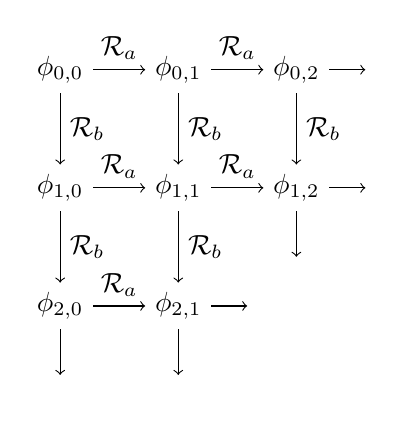
\begin{tikzpicture}[node distance=1.5cm, auto]
  \node (phi00) {$\phi_{0,0}$};
  \node (phi01) [right of=phi00] {$\phi_{0,1}$};
  \node (phi02) [right of=phi01] {$\phi_{0,2}$};
  \node (phi03) [right of=phi02, node distance=1cm] {$ $};

  \node (phi10) [below of=phi00] {$\phi_{1,0}$};
  \node (phi11) [right of=phi10] {$\phi_{1,1}$};
  \node (phi12) [right of=phi11] {$\phi_{1,2}$};
  \node (phi13) [right of=phi12, node distance=1cm] {$ $};

  \node (phi20) [below of=phi10] {$\phi_{2,0}$};
  \node (phi21) [right of=phi20] {$\phi_{2,1}$};
  \node (phi22a) [right of=phi21, node distance=1cm] {$ $};
  \node (phi22b) [below of=phi12, node distance=1cm] {$ $};

  \node (phi30) [below of=phi20, node distance=1cm] {$ $};
  \node (phi31) [below of=phi21, node distance=1cm] {$ $};

  \draw[->] (phi00) to node {$\mathcal{R}_a$} (phi01);
  \draw[->] (phi01) to node {$\mathcal{R}_a$} (phi02);
  \draw[->] (phi02) to node {$ $} (phi03);

  \draw[->] (phi10) to node {$\mathcal{R}_a$} (phi11);
  \draw[->] (phi11) to node {$\mathcal{R}_a$} (phi12);
  \draw[->] (phi12) to node {$ $} (phi13);

  \draw[->] (phi20) to node {$\mathcal{R}_a$} (phi21);
  \draw[->] (phi21) to node {$ $} (phi22a);

  \draw[->] (phi00) to node {$\mathcal{R}_b$} (phi10);
  \draw[->] (phi10) to node {$\mathcal{R}_b$} (phi20);
  \draw[->] (phi20) to node {$ $} (phi30);

  \draw[->] (phi01) to node {$\mathcal{R}_b$} (phi11);
  \draw[->] (phi11) to node {$\mathcal{R}_b$} (phi21);
  \draw[->] (phi21) to node {$ $} (phi31);

  \draw[->] (phi02) to node {$\mathcal{R}_b$} (phi12);
  \draw[->] (phi12) to node {$ $} (phi22b);
\end{tikzpicture}

  \caption{The grid of basis functions $\phi_{k,l}$ for the case $D=2$.}
  \label{fig:phi_kl_grid}
\end{figure}

Every arrow stands for a raising operator $\mathcal{R}$ and we see that there are
two kinds of arrows, vertical and horizontal ones. Following an arrow only one
of the two indices $(k,l)$ changes. This is shown in more details in figure
\ref{fig:phi_kl_operators}.

\begin{figure}[h!]
  \centering
  \subfloat[][]{
    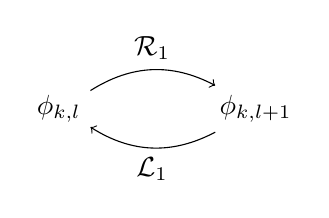
\begin{tikzpicture}[node distance=2.5cm, auto]
  \node (phikl) {$\phi_{k,l}$};
  \node (phikll) [right of=phikl] {$\phi_{k,l+1}$};
  \draw[->] (phikl) to [bend left] node {$\mathcal{R}_1$} (phikll);
  \draw[->] (phikll) to [bend left] node {$\mathcal{L}_1$} (phikl);
\end{tikzpicture}

  }
  \subfloat[][]{
    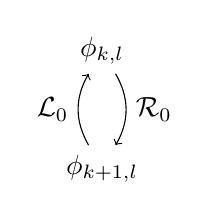
\begin{tikzpicture}[node distance=1.5cm, auto]
  \node (phikl) {$\phi_{k,l}$};
  \node (phikkl) [below of=phikl] {$\phi_{k+1,l}$};
  \draw[->] (phikl) to [bend left] node {$\mathcal{R}_0$} (phikkl);
  \draw[->] (phikkl) to [bend left] node {$\mathcal{L}_0$} (phikl);
\end{tikzpicture}

  } \\
    \caption[]{The two raising and lowering operator pairs in action.}
    \label{fig:phi_kl_operators}
\end{figure}

This fact suggests that we assign a raising operator to each arrow type hence we
get two operators $\mathcal{R}_0$ and $\mathcal{R}_1$ which are of different
nature. We can assign a distinct set $\{\mathcal{R}_i, \mathcal{L}_i\}$ to each
axis $i \in [0, \ldots, D-1]$ of the lattice.

Leaving this introductionary example and following the formal derivation from
\cite{H_ladder_operators} now, we take $\vec{v} \in \mathbb{C}^D$, define
$\vec{y} \assign -i \varepsilon^2 \nabla_x$ and begin with:

\begin{align}
  \mathcal{R}_v & \assign \frac{1}{\sqrt{2\varepsilon^2}}
                  \left(
                    \dotp{-i\mat{P}\vec{\conj{v}}}{(\vec{x}-\vec{q})}
                    -i \dotp{\mat{Q}\vec{\conj{v}}}{(\vec{y}-\vec{p})}
                  \right) \\
                & = \frac{1}{\sqrt{2\varepsilon^2}}
                  \left(
                    i \dotp{\mat{P}\vec{\conj{v}}}{(\vec{x}-\vec{q})}
                    -i \dotp{\mat{Q}\vec{\conj{v}}}{(\vec{y}-\vec{p})}
                  \right) \\
                & = \frac{i}{\sqrt{2\varepsilon^2}}
                  \left(
                    \dotp{\mat{P}\vec{\conj{v}}}{(\vec{x}-\vec{q})}
                    - \dotp{\mat{Q}\vec{\conj{v}}}{(\vec{y}-\vec{p})}
                  \right)
\end{align}

and similarly we get:

\begin{align}
  \mathcal{L}_v & \assign \frac{1}{\sqrt{2\varepsilon^2}}
                  \left(
                    \dotp{\conj{-i \mat{P}}\vec{v}}{(\vec{x}-\vec{q})}
                    +i \dotp{\mat{\conj{Q}}\vec{v}}{(\vec{y}-\vec{p})}
                  \right) \\
                & = \frac{1}{\sqrt{2\varepsilon^2}}
                  \left(
                    -i \dotp{\mat{\conj{P}}\vec{v}}{(\vec{x}-\vec{q})}
                    +i \dotp{\mat{\conj{Q}}\vec{v}}{(\vec{y}-\vec{p})}
                  \right) \\
                & = -\frac{i}{\sqrt{2\varepsilon^2}}
                  \left(
                    \dotp{\mat{\conj{P}}\vec{v}}{(\vec{x}-\vec{q})}
                    - \dotp{\mat{\conj{Q}}\vec{v}}{(\vec{y}-\vec{p})}
                  \right) \,.
\end{align}

For the one-dimensional case we can get back at the definitions from \eqref{eq:raising_ops_1d}.
Following along the lines of \cite{H_ladder_operators} we can compute several commutators:

\begin{align}
  [\mathcal{L}_v, \mathcal{L}_w] & = \mathcal{L}_v\mathcal{L}_w - \mathcal{L}_w\mathcal{L}_v = 0 \\
  [\mathcal{R}_v, \mathcal{R}_w] & = \mathcal{R}_v\mathcal{R}_w - \mathcal{R}_w\mathcal{R}_v = 0 \\
  [\mathcal{L}_v, \mathcal{R}_w] & = \mathcal{L}_v\mathcal{R}_w - \mathcal{R}_w\mathcal{L}_v = \dotp{\vec{v}}{\vec{w}}
\end{align}

for general $\vec{v}, \vec{w} \in \mathbb{C}^D$. The fact that we are allowed to
interchange two raising operators is important and could have been guessed from
figure \ref{fig:phi_kl_grid}. There we have:

\begin{align*}
  \phi_{1,1} & = \mathcal{R}_0 \phi_{0,1} = \mathcal{R}_0 \mathcal{R}_1 \phi_{0,0} \\
  \phi_{1,1} & = \mathcal{R}_1 \phi_{1,0} = \mathcal{R}_1 \mathcal{R}_0 \phi_{0,0}
\end{align*}

thus the order in which we compute $\phi_{k,l}$ from $\phi_{0,0}$ does not matter.
If we flip all arrows we get to the same conclusion but this time for lowering
operators.

From the scalar case we know that we can not simply exchange two different
operators, remember for example the definition of the number operator $\mathcal{N}$.
However, we can go from $\phi_{1,0}$ to $\phi_{0,1}$ by either way:

\begin{align*}
  \phi_{0,1} & = \mathcal{L}_0 \phi_{1,1} = \mathcal{L}_0 \mathcal{R}_1 \phi_{1,0} \\
  \phi_{0,1} & = \mathcal{R}_1 \phi_{0,0} = \mathcal{R}_1 \mathcal{L}_0 \phi_{1,0} \,.
\end{align*}

This is the consequence of the third commutation relation above which tells us
that the two operators commute iff $\vec{v}$ and $\vec{w}$ are orthogonal.

Continuing with the formal derivation we choose a basis of $\mathbb{R}^D$. For
simplicity we take the canonical basis $\{\vec{e}^j\}_{j=0}^{D-1}$. In this basis
we can more precisely say what $\mathcal{R}_v$ is. We define the following two
sets of ladder operators:

\begin{align}
  \mathcal{R}_j & \assign \mathcal{R}_{e^j} \\
  \mathcal{L}_j & \assign \mathcal{L}_{e^j}
\end{align}

each containing exactly $D$ operators. Finally we can build the vector-valued
operators:

\begin{equation} \label{eq:raising_ops_Dd_vectorial}
  \mathcal{R} \assign
  \begin{pmatrix}
    \mathcal{R}_0 \\
    \vdots \\
    \mathcal{R}_{D-1}
  \end{pmatrix}
  \qquad \text{and} \qquad
  \mathcal{L} \assign
  \begin{pmatrix}
    \mathcal{L}_0 \\
    \vdots \\
    \mathcal{L}_{D-1}
  \end{pmatrix} \,.
\end{equation}

Recalling the defining equations for $\mathcal{R}_v$ and $\mathcal{L}_v$ we can
then find explicit expressions for $\mathcal{R}$ and $\mathcal{L}$:

\begin{align} \label{eq:raising_ops_Dd_explicit}
  \mathcal{R} & =  \frac{i}{\sqrt{2\varepsilon^2}} \left( \mat{P}\H (\vec{x}-\vec{q}) - \mat{Q}\H (\vec{y}-\vec{p}) \right) \\
  \mathcal{L} & = -\frac{i}{\sqrt{2\varepsilon^2}} \left( \mat{P}\T (\vec{x}-\vec{q}) - \mat{Q}\T (\vec{y}-\vec{p}) \right) \,.
\end{align}

At this point we should stop for a moment and see what happens if we set $D=1$ now.
If we carried out all calculations we would return step by step to the expressions
given in \eqref{eq:raising_ops_1d}.

With the help of $\mathcal{R}$ we can now go on and define all higher states
$\phi_{\vec{k}}$ properly:

\begin{align} \label{eq:construct_phi_k}
  \phi_{\vec{k}} & \assign \mathcal{R}^{\vec{k}} \phi_{\vec{0}} \\
                 & = \frac{1}{\sqrt{\vec{k}!}} \mathcal{R}_0^{k_0} \mathcal{R}_1^{k_1} \cdots \mathcal{R}_{D-1}^{k_{D-1}} \phi_{\vec{0}} \\
                 & = \frac{1}{\sqrt{\prod_{i=0}^{D-1}k_i!}} \prod_{i=0}^{D-1} \mathcal{R}_i^{k_i} \phi_{\vec{0}} \,.
\end{align}

We can show theorem 3.3 of \cite{H_ladder_operators}:

\begin{theorem}
  The functions $\phi_{\vec{k}}\left[\Pi\right](\vec{x})$ form an orthonormal
  basis of $L^2 \left(\mathbb{R}^D \right)$.
\end{theorem}

For a proof see again this reference.

To close this section we take a closer look at the application of $\mathcal{R}_j$
on $\phi_{\vec{k}}$:

\begin{equation} \label{eq:r_op_applied_1}
  \mathcal{R}_j \phi_{\vec{k}} = \sqrt{k_j + 1} \phi_{\vec{k}^\prime}
\end{equation}

where:

\begin{equation}
  \vec{k}^\prime \assign \vec{k} + \vec{e}^j = (k_0, \ldots, k_{j-1}, k_j+1, k_{j+1}, \ldots, k_{D-1})
\end{equation}

and similarly:

\begin{equation}
  \mathcal{L}_j \phi_{\vec{k}} = \sqrt{k_j} \phi_{\vec{k}^\prime}
\end{equation}

with:

\begin{equation}
  \vec{k}^\prime \assign \vec{k} - \vec{e}^j = (k_0, \ldots, k_{j-1}, k_j-1, k_{j+1}, \ldots, k_{D-1}) \,.
\end{equation}

This justifies the formula \eqref{eq:construct_phi_k} allowing us to construct
$\phi_{\vec{k}}$ out of $\phi_{\vec{0}}$ by raising each index multiple times as
necessary. We build a path through the lattice starting at the origin and ending
at the point $\vec{k}$.

From these formula we see that computing $\mathcal{R} \phi_{\vec{0}}$ is sufficient
to access all higher order functions. The remaining question is how to do this
efficiently. Computing the action of $\mathcal{R}$ is not straight forward because
it contains the differential operator $y \assign -i \varepsilon^2 \nabla_x$. For
this reason we seek a way to compute $\mathcal{R} \phi_{\vec{0}}$ without
ever applying $y$ explicitly. The solution to this task is given by the adjoint
pair $\mathcal{R}, \mathcal{L}$ of operators. We can set up a system of two
operator equations. First we solve the equation defining $\mathcal{L}$ for $y$.
For simplicity of notation we define $\theta \assign \frac{i}{\sqrt{2\varepsilon^2}}$
and transform as follows:

\begin{align} \label{eq:y_op}
  \mathcal{L} & = -\theta \left( \mat{P}\T (\vec{x}-\vec{q}) - \mat{Q}\T (\vec{y}-\vec{p}) \right) \nonumber\\
  \mathcal{L} & = -\theta \mat{P}\T (\vec{x}-\vec{q}) + \theta \mat{Q}\T (\vec{y}-\vec{p}) \nonumber\\
  \mathcal{L} + \theta \mat{P}\T (\vec{x}-\vec{q}) & = \theta \mat{Q}\T (\vec{y}-\vec{p}) \nonumber\\
  \mat{Q}\T (\vec{y}-\vec{p}) & = \frac{1}{\theta} \mathcal{L} + \mat{P}\T (\vec{x}-\vec{q}) \nonumber\\
  \vec{y}-\vec{p} & = \frac{1}{\theta} \mat{Q}\Tinv \mathcal{L} + \mat{Q}\Tinv \mat{P}\T (\vec{x}-\vec{q}) \nonumber\\
  \vec{y} & = \frac{1}{\theta} \mat{Q}\Tinv \mathcal{L} + \mat{Q}\Tinv \mat{P}\T (\vec{x}-\vec{q}) + \vec{p} \,.
\end{align}

Note that solving $\mathcal{R}$ for $y$ gives us the complex conjugate of this
last line:

\begin{equation}  \label{eq:y_op_cc}
  \vec{y} = -\frac{1}{\theta} \mat{Q}\Hinv \mathcal{R} + \mat{Q}\Hinv \mat{P}\H (\vec{x}-\vec{q}) + \vec{p} \,.
\end{equation}

In the next step we plug the result \eqref{eq:y_op} into the definition of
$\mathcal{R}$:

\begin{align} \label{eq:loc_op_r}
  \mathcal{R} & = \theta \left( \mat{P}\H (\vec{x}-\vec{q}) - \mat{Q}\H (\vec{y}-\vec{p}) \right) \nonumber\\
  \mathcal{R} & = \theta \left( \mat{P}\H (\vec{x}-\vec{q}) - \mat{Q}\H \left(\left(
                  \frac{1}{\theta} \mat{Q}\Tinv \mathcal{L} + \mat{Q}\Tinv \mat{P}\T (\vec{x}-\vec{q}) + \vec{p}
                  \right)-\vec{p}\right) \right) \nonumber\\
  \mathcal{R} & = \theta \left( \mat{P}\H (\vec{x}-\vec{q}) - \mat{Q}\H \left(
                  \frac{1}{\theta} \mat{Q}\Tinv \mathcal{L} + \mat{Q}\Tinv \mat{P}\T (\vec{x}-\vec{q})
                  \right) \right) \nonumber\\
  \mathcal{R} & = \theta \left( \mat{P}\H (\vec{x}-\vec{q})
                    - \frac{1}{\theta} \mat{Q}\H\mat{Q}\Tinv \mathcal{L}
                    - \mat{Q}\H\mat{Q}\Tinv\mat{P}\T (\vec{x}-\vec{q})
                  \right) \nonumber\\
  \mathcal{R} & = \theta \left(
                    - \frac{1}{\theta} \mat{Q}\H\mat{Q}\Tinv \mathcal{L}
                    + \underbrace{(\mat{P}\H - \mat{Q}\H\mat{Q}\Tinv\mat{P}\T)}_{*} (\vec{x}-\vec{q})
                  \right) \,.
\end{align}

This is already quite useful a result. But let's see if we can simplify the
underbraced part further. Simplifying the $*$ part needs a bit of algebra. We
start with the basic relations in \eqref{eq:PQcond_Dd} and multiply the first
one by $\mat{Q}\inv$ from the right:

\begin{align*}
  \mat{Q}\H \mat{P} - \mat{P}\H \mat{Q} & = 2i \id \\
  \mat{Q}\H \mat{P} \mat{Q}\inv - \mat{P}\H \mat{Q} \mat{Q}\inv & = 2i \mat{Q}\inv \\
  \mat{Q}\H \mat{P} \mat{Q}\inv - \mat{P}\H & = 2i \mat{Q}\inv \\
  \mat{P}\H - \mat{Q}\H \underbrace{\mat{P} \mat{Q}\inv}_{**} & = -2i \mat{Q}\inv \,.
\end{align*}

Now we are left with $**$ where we can apply the other fundamental relation which
we have to transform a little bit first:

\begin{align*}
  \mat{P}\T \mat{Q} - \mat{Q}\T \mat{P} & = \mat{0} \\
  \mat{Q}\Tinv \mat{P}\T \mat{Q} - \mat{Q}\Tinv \mat{Q}\T \mat{P} & = \mat{0} \\
  \mat{Q}\Tinv \mat{P}\T \mat{Q} & = \mat{P} \,.
\end{align*}

The last line can now be used to replace the $\mat{P}$ in $**$ which yields:

\begin{align*}
  \mat{P}\H - \mat{Q}\H \mat{Q}\Tinv \mat{P}\T \mat{Q} \mat{Q}\inv & = -2i \mat{Q}\inv \\
  \mat{P}\H - \mat{Q}\H \mat{Q}\Tinv \mat{P}\T & = -2i \mat{Q}\inv \,.
\end{align*}

This is the part $*$ we wanted to simplify. Going back to \eqref{eq:loc_op_r}
we can write:

\begin{align*}
  \mathcal{R} & = \theta \left(
                    - \frac{1}{\theta} \mat{Q}\H\mat{Q}\Tinv \mathcal{L}
                    -2i \mat{Q}\inv (\vec{x}-\vec{q})
                  \right) \\
  \mathcal{R} & = - \mat{Q}\H\mat{Q}\Tinv \mathcal{L}
                    -2i \theta \mat{Q}\inv (\vec{x}-\vec{q}) \,.
\end{align*}

At the end of the day we get:

\begin{equation} \label{eq:r_op_wo_deriv}
  \boxed{
    \mathcal{R} = \sqrt{\frac{2}{\varepsilon^2}} \mat{Q}\inv (\vec{x}-\vec{q}) - \mat{Q}\H\mat{Q}\Tinv \mathcal{L}
  }
\end{equation}

where we reinserted the term for $\theta$ and took into account the $i$ therein.
Of course we would get the very same result if we used \eqref{eq:y_op_cc} and
plugged it into the definition of $\mathcal{L}$. Just for the sake of completeness
we state the complex conjugate result for the $\mathcal{L}$ operator too:

\begin{equation}
  \boxed{
    \mathcal{L} = \sqrt{\frac{2}{\varepsilon^2}} \mat{\conj{Q}}\inv (\vec{x}-\vec{q}) - \mat{Q}\T\mat{Q}\Hinv \mathcal{R}
  }
\end{equation}

with a similar derivation as the one above.


\section{Higher order basis functions}


With this equation at hand we can continue in \eqref{eq:r_op_applied_1} where we
left off computing $\mathcal{R}_d \phi_{\vec{k}}$. We start applying the operator
for the $d$-th direction. But we do not have an explicit expression for
$\mathcal{R}_d$ and on the other hand we need the result for all $d \in [0, \ldots, D-1]$.
Therefore is seems wise to do these computations simultaneously for all $D$ components:

\begin{align}
  \begin{pmatrix}
    \sqrt{k_0 + 1} \phi_{\vec{k}+\vec{e}^0} \\
    \vdots \\
    \sqrt{k_{D-1} + 1} \phi_{\vec{k}+\vec{e}^{D-1}}
  \end{pmatrix}
  =
  \begin{pmatrix}
    \mathcal{R}_0 \phi_{\vec{k}} \\
    \vdots \\
    \mathcal{R}_{D-1} \phi_{\vec{k}}
  \end{pmatrix}
  =
  \mathcal{R} \phi_{\vec{k}}
\end{align}

Using the formula \eqref{eq:r_op_wo_deriv} for $\mathcal{R}$ gives us:

\begin{equation} \label{eq:basis_recursion_DD}
  \begin{pmatrix}
    \sqrt{k_0+1} \, \phi_{\vec{k}+\vec{e}^0} \\
    \vdots \\
    \sqrt{k_{D-1}+1} \, \phi_{\vec{k}+\vec{e}^{D-1}}
  \end{pmatrix}
  =
  \sqrt{\frac{2}{\varepsilon^2}} \mat{Q}\inv (\vec{x}-\vec{q}) \phi_{\vec{k}}
  - \mat{Q}\H\mat{Q}\Tinv
  \begin{pmatrix}
    \sqrt{k_0} \phi_{\vec{k}-\vec{e}^0} \\
    \vdots \\
    \sqrt{k_{D-1}} \phi_{\vec{k}-\vec{e}^{D-1}}
  \end{pmatrix} \,.
\end{equation}

From this we get the new functions $\phi_{\vec{k}+\vec{e}^d}$ as:

\begin{equation*}
  \begin{pmatrix}
    \phi_{\vec{k}+\vec{e}^0} \\
    \vdots \\
    \phi_{\vec{k}+\vec{e}^{D-1}}
  \end{pmatrix}
  = \left(
  \sqrt{\frac{2}{\varepsilon^2}} \mat{Q}\inv (\vec{x}-\vec{q}) \phi_{\vec{k}}
  - \mat{Q}\H\mat{Q}\Tinv
  \begin{pmatrix}
    \sqrt{k_0} \phi_{\vec{k}-\vec{e}^0} \\
    \vdots \\
    \sqrt{k_{D-1}} \phi_{\vec{k}-\vec{e}^{D-1}}
  \end{pmatrix}
  \right)
  \oslash
  \begin{pmatrix}
    \sqrt{k_0+1}\\
    \vdots \\
    \sqrt{k_{D-1}+1}
  \end{pmatrix}
\end{equation*}

where the operator $\oslash$ denotes component-wise division. In a next step
we use this formula for evaluation of all $\phi_{\vec{k}}$ basis functions
of $D$ dimensional semi-classical wavepackets. This last formula is so important
that it should carry a box too but it seems there is no space left.


\begin{figure}
  \centering
  \subfloat[][]{
    \label{fig:phi_00}
    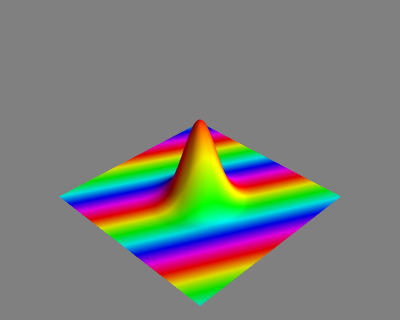
\includegraphics[width=0.5\linewidth]{./fig/phi/phi_0-0.png}
  }
  \subfloat[][]{
    \label{fig:phi_10}
    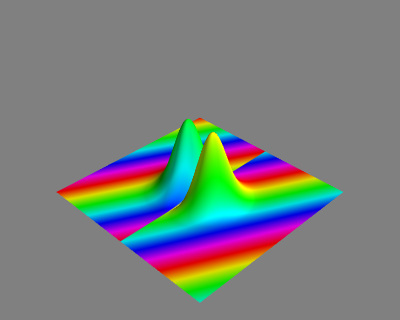
\includegraphics[width=0.5\linewidth]{./fig/phi/phi_1-0.png}
  } \\
  \subfloat[][]{
    \label{fig:phi_01}
    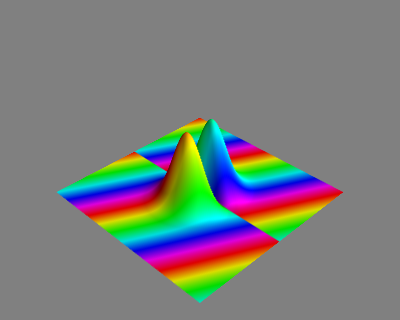
\includegraphics[width=0.5\linewidth]{./fig/phi/phi_0-1.png}
  }
  \subfloat[][]{
    \label{fig:phi_11}
    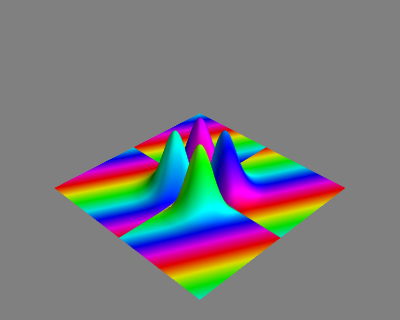
\includegraphics[width=0.5\linewidth]{./fig/phi/phi_1-1.png}
  } \\
  \subfloat[][]{
    \label{fig:phi_02}
    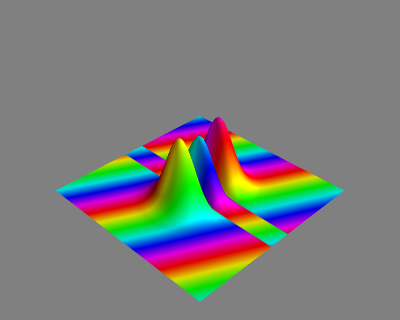
\includegraphics[width=0.5\linewidth]{./fig/phi/phi_0-2.png}
  }
  \subfloat[][]{
    \label{fig:phi_12}
    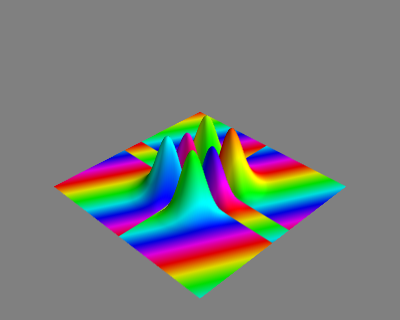
\includegraphics[width=0.5\linewidth]{./fig/phi/phi_1-2.png}
  } \\
  \caption[Plots of some basis functions $\phi$]{
    Plots of the first few functions $\phi_{k,l}$ with parameters set
    to $\vec{q} = \vec{0}$, $\vec{p} = (1, \frac{1}{2})$, $\mat{Q} = \id$, $\mat{P} = i \id$
    and $\varepsilon = 1$. The surface represents ten times the value
    $\sqrt{\Braket{\phi_{k,l}|\phi_{k,l}}}$ where the factor of $10$
    is just for visual purpose. For an explanation of the colours, see appendix \ref{ch:color_code}.
    \subref{fig:phi_00} $\phi_{0,0}$
    \subref{fig:phi_10} $\phi_{1,0}$
    \subref{fig:phi_01} $\phi_{0,1}$
    \subref{fig:phi_11} $\phi_{1,1}$
    \subref{fig:phi_02} $\phi_{0,2}$
    \subref{fig:phi_12} $\phi_{1,2}$
    \label{fig:phi_table_1}
  }
\end{figure}


\begin{figure}
  \centering
  \subfloat[][]{
    \label{fig:phi_20}
    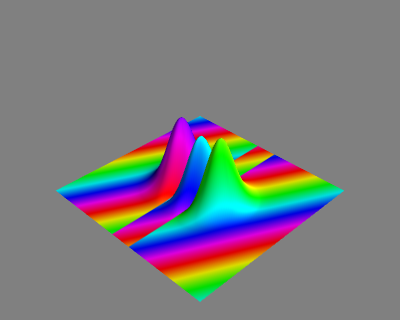
\includegraphics[width=0.5\linewidth]{./fig/phi/phi_2-0.png}
  }
  \subfloat[][]{
    \label{fig:phi_30}
    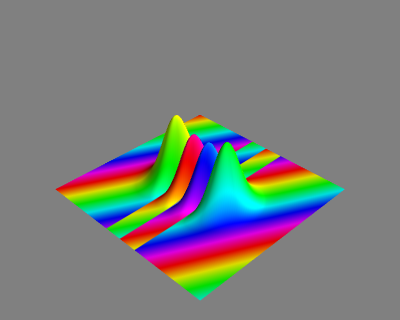
\includegraphics[width=0.5\linewidth]{./fig/phi/phi_3-0.png}
  } \\
  \subfloat[][]{
    \label{fig:phi_21}
    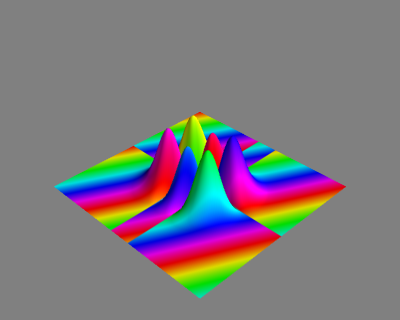
\includegraphics[width=0.5\linewidth]{./fig/phi/phi_2-1.png}
  }
  \subfloat[][]{
    \label{fig:phi_31}
    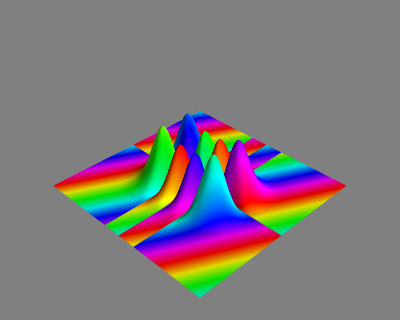
\includegraphics[width=0.5\linewidth]{./fig/phi/phi_3-1.png}
  } \\
  \subfloat[][]{
    \label{fig:phi_22}
    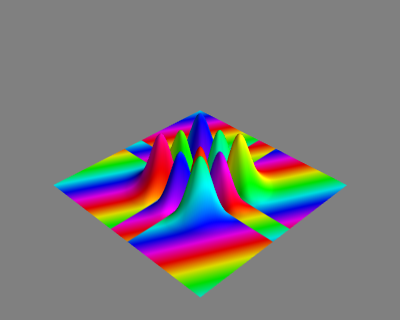
\includegraphics[width=0.5\linewidth]{./fig/phi/phi_2-2.png}
  }
  \subfloat[][]{
    \label{fig:phi_32}
    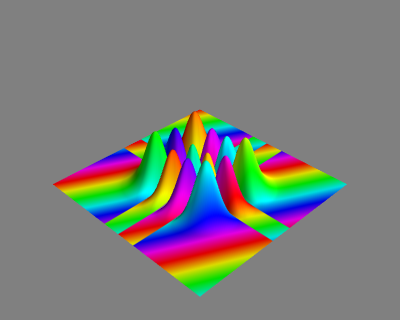
\includegraphics[width=0.5\linewidth]{./fig/phi/phi_3-2.png}
  } \\
  \caption[Plots of some basis functions $\phi$]{
    Plots of the first few functions $\phi_{k,l}$ with parameters set
    to $\vec{q} = \vec{0}$, $\vec{p} = (1, \frac{1}{2})$, $\mat{Q} = \id$, $\mat{P} = i \id$
    and $\varepsilon = 1$. The surface represents ten times the value
    $\sqrt{\Braket{\phi_{k,l}|\phi_{k,l}}}$ where the factor of $10$
    is just for visual purpose. For an explanation of the colours, see appendix \ref{ch:color_code}.
    \subref{fig:phi_20} $\phi_{2,0}$
    \subref{fig:phi_30} $\phi_{3,0}$
    \subref{fig:phi_21} $\phi_{2,1}$
    \subref{fig:phi_31} $\phi_{3,1}$
    \subref{fig:phi_22} $\phi_{2,2}$
    \subref{fig:phi_32} $\phi_{3,2}$
    \label{fig:phi_table_2}
  }
\end{figure}


\section{Construction of wavepackets}


In the previous section we saw how to compute the functions $\phi_{\vec{k}}[\Pi](\vec{x})$.
Now we can take a very general set $\mathfrak{K}$ of indices $\vec{k}$ and use
the corresponding functions $\phi_{\vec{k}}$ to build a (more or less truncated)
basis for $L^2(\mathbb{R}^D)$. In a first step we can construct so called
\emph{scalar wavepackets} $\Phi$ by linear combinations:

\begin{equation}
  \Phi(\vec{x}) \assign \exp\left(\frac{i S}{\varepsilon^2}\right) \sum_{\vec{k}\in\mathfrak{K}} c_{\vec{k}} \phi_{\vec{k}}
\end{equation}

where the coefficients $c_{\vec{k}} \in \mathbb{C}$ depend on time only and the basis functions
$\phi_{\vec{k}}$ depend on space but also on time through the parameter set
$\Pi(t)$ which is time-dependent\footnote{In general we neglect explicit
time-dependence of the parameter set $\Pi$ in our notation.}. We added a global
phase $S$ which is also time-dependent. An overly precise notation reads:

\begin{definition}[Scalar semi-classical wavepacket]
  \begin{equation} \label{eq:scalar_wavepacket}
    \Ket{\Phi} \assign
    \Phi\left[\Pi(t)\right](\vec{x}, t)
    =
    \exp\left(\frac{i S(t)}{\varepsilon^2}\right) \sum_{\vec{k}\in\mathfrak{K}} c_{\vec{k}}(t) \phi_{\vec{k}}\left[\Pi(t)\right](\vec{x}) \,.
  \end{equation}
\end{definition}

Every single basis function $\phi_{\vec{k}}$ is a perfectly valid wavepacket too.
Sometimes we will append the parameter $S$ to the set $\Pi$ and use the notation
$\Pi = \{q,p,Q,P,S\}$. This should be clear from the context. Also we will drop
the time variable since we look at wavepackets at fixed times.


\section{Basis set expansion and basis shapes}


The above formulation is a basis expansion for the true wavefunction $\varphi(\vec{x}, t)$.
Remember that the set $\{\phi_{\vec{k}}\}_{\vec{k}\in\mathfrak{K}}$ is a (complete)
basis of the function space $L^2(\mathbb{R}^D)$. Hence the basis expansion is
exact if we take the full lattice $\mathfrak{K} = \mathbb{N}_0^D$ of indices. In
theoretical considerations we can use the full lattice but for all practical
purposes we need to truncate the basis and make the set $\mathfrak{K}$ finite.
This can be done in various ways and we refer to the \emph{shape} of a basis set
if we speak about these details of $\mathfrak{K}$. Basis shapes usually depend
on some parameters $\theta$, we occasionally write $\mathfrak{K}(\theta)$ for this.

For a first ansatz we can use a hypercubic basis set $\mathfrak{K}$ which means
that we take the subset of all lattice points for which $\vec{k} < \vec{K}$ holds.
The components of $\vec{K}$ specify the number of points along each of the $D$
directions. A more formal definition is:

\begin{definition}[Hypercubic basis shape]
  \begin{equation}
    \mathfrak{K}(\vec{K}) \assign \left\{ \vec{k} \in \mathbb{N}_0^D :
                                          \, k_d < K_d \,\forall\, d \in [0, \ldots, D-1] \right\} \,.
  \end{equation}
\end{definition}

If we use this basis shape we call the resulting wavepacket \emph{dense}. By
$|\mathfrak{K}|$ we denote the \emph{basis size}, the overall number of basis
functions $\phi_{\vec{k}}$ we use. In the hypercubic case this is obviously:

\begin{equation}
  |\mathfrak{K}| = \prod_{d=0}^{D-1} K_d \,.
\end{equation}

As a shorthand notation to specify the hypercubic shape we simply write
$\mathfrak{K} = \vec{K} = [K_0, \ldots, K_{D-1}]$. We should think of $\vec{K}$ as
being both the vector in the lattice $\mathbb{N}_0^D$ and the set of all index
points in the hypercube spanned by the origin $\vec{0} = (0, \ldots, 0)$ and
$\vec{K} - \vec{1} = (K_0-1, \ldots, K_{D-1}-1)$, depending on the context.

The size of this basis shape grows exponentially with the number $D$ of dimensions.
Therefore we introduce more sparse basis sets which grow slower as the number
of dimensions increases. The first example is the \emph{hyperbolic cut} basis shape
defined as follows:

\begin{definition}[Hyperbolic cut basis shape] \label{def:hyperbolic_cut_shape}
  \begin{equation}
    \mathfrak{K}(K) \assign \left\{ \vec{k} \in \mathbb{N}_0^D :
                                    \, \prod_{d=0}^{D-1}(1+k_d) \leq K \right\}
  \end{equation}
\end{definition}

where we limit the number of basis functions by hyperbolic cuts. For this we
introduce a scalar parameter $K \in \mathbb{N}$ which we call \emph{sparsity}
in this context. The number of basis functions is then bounded by:

\begin{equation}
  |\mathfrak{K}| \leq \mathcal{C} K \left(\log K\right)^{D-1} \,.
\end{equation}

where $\mathcal{C}$ is some constant.

Figure \ref{fig:hyperbolic_cut_basis_size} shows the application of this bound
to the two-dimensional case.

\begin{figure}
  \centering
  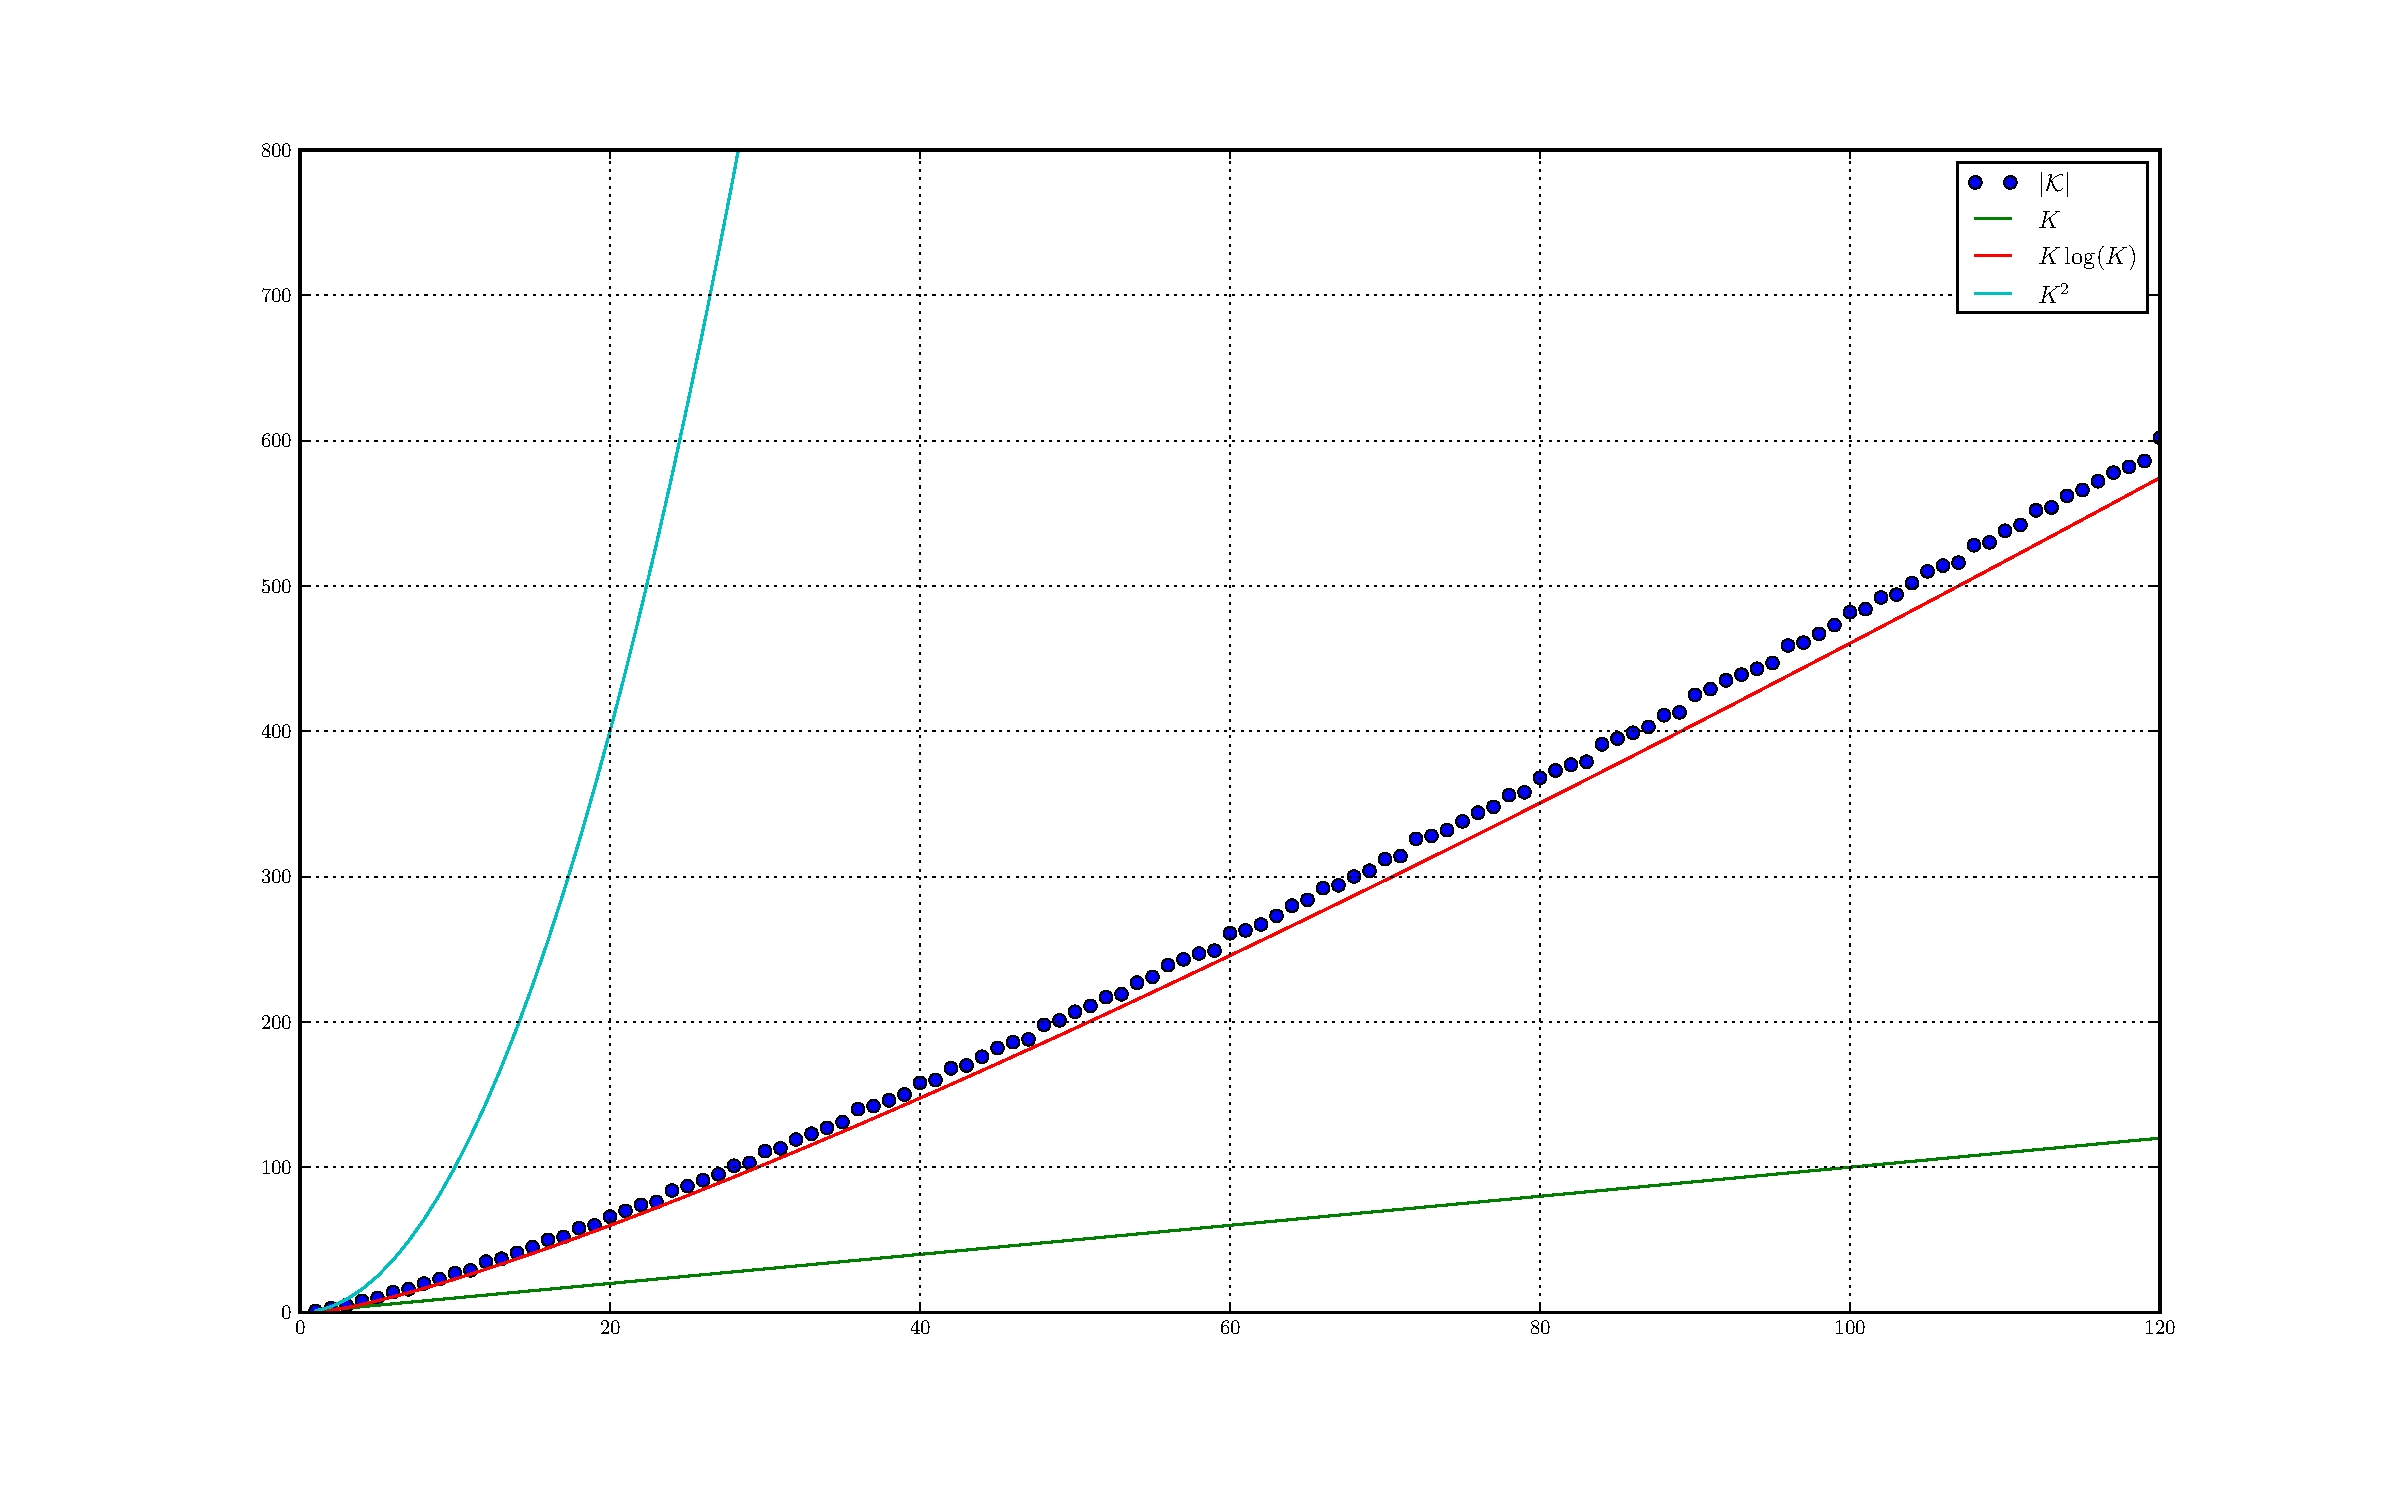
\includegraphics[width=0.8\linewidth]{./fig/basis_size.pdf}
  \caption{The size $|\mathfrak{K}|$ of two-dimensional hyperbolic basis shapes
           with various cut-off values $K$.}
  \label{fig:hyperbolic_cut_basis_size}
\end{figure}

\begin{figure}
  \centering
  \subfloat[][]{
    \label{fig:hyperbolic_cut_2_8}
    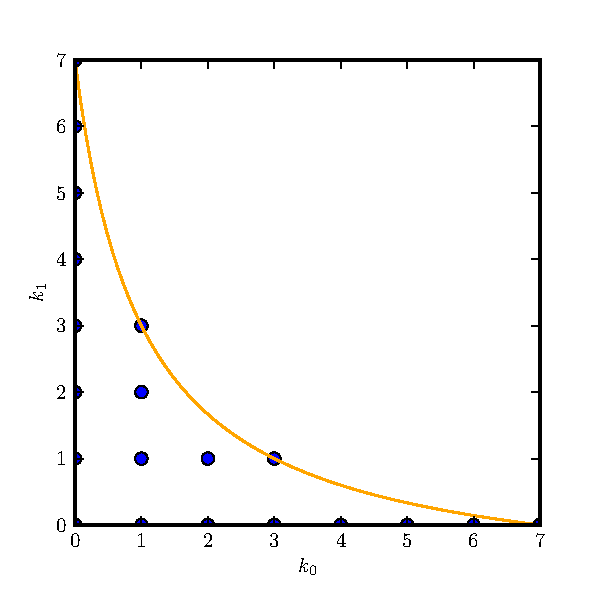
\includegraphics[width=0.5\linewidth]{./fig/hyperbolic_shape_2_8.pdf}
  }
  \subfloat[][]{
    \label{fig:hyperbolic_cut_2_32}
    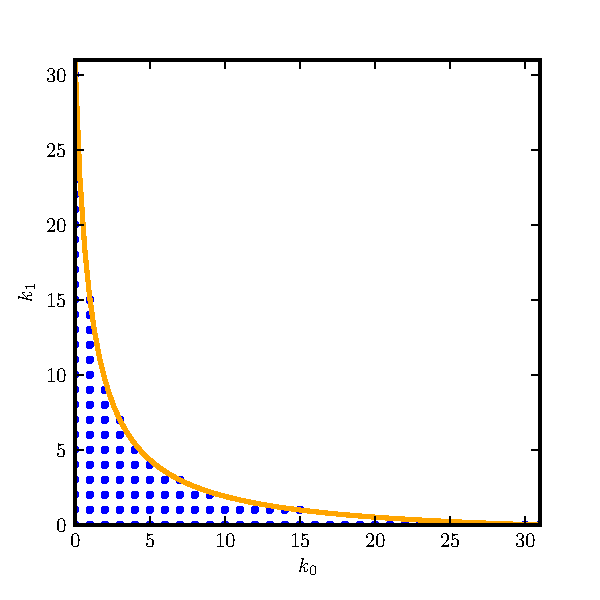
\includegraphics[width=0.5\linewidth]{./fig/hyperbolic_shape_2_32.pdf}
  } \\
  \caption[Hyperbolic cut basis shape in two dimensions]{
    The lattice nodes that are part of a two-dimensional hyperbolic cut basis
    shape. Additionally the cut-off function is shown. Compared to the full
    hypercubic basis shape the sparsity of this type of basis shape becomes
    clearly visible.
    \subref{fig:hyperbolic_cut_2_8} $K = 8$
    \subref{fig:hyperbolic_cut_2_32} $K = 32$
    \label{fig:hyperbolic_cut_2D}
  }
\end{figure}

\begin{figure}
  \centering
  \subfloat[][]{
    \label{fig:hyperbolic_cut_3_8}
    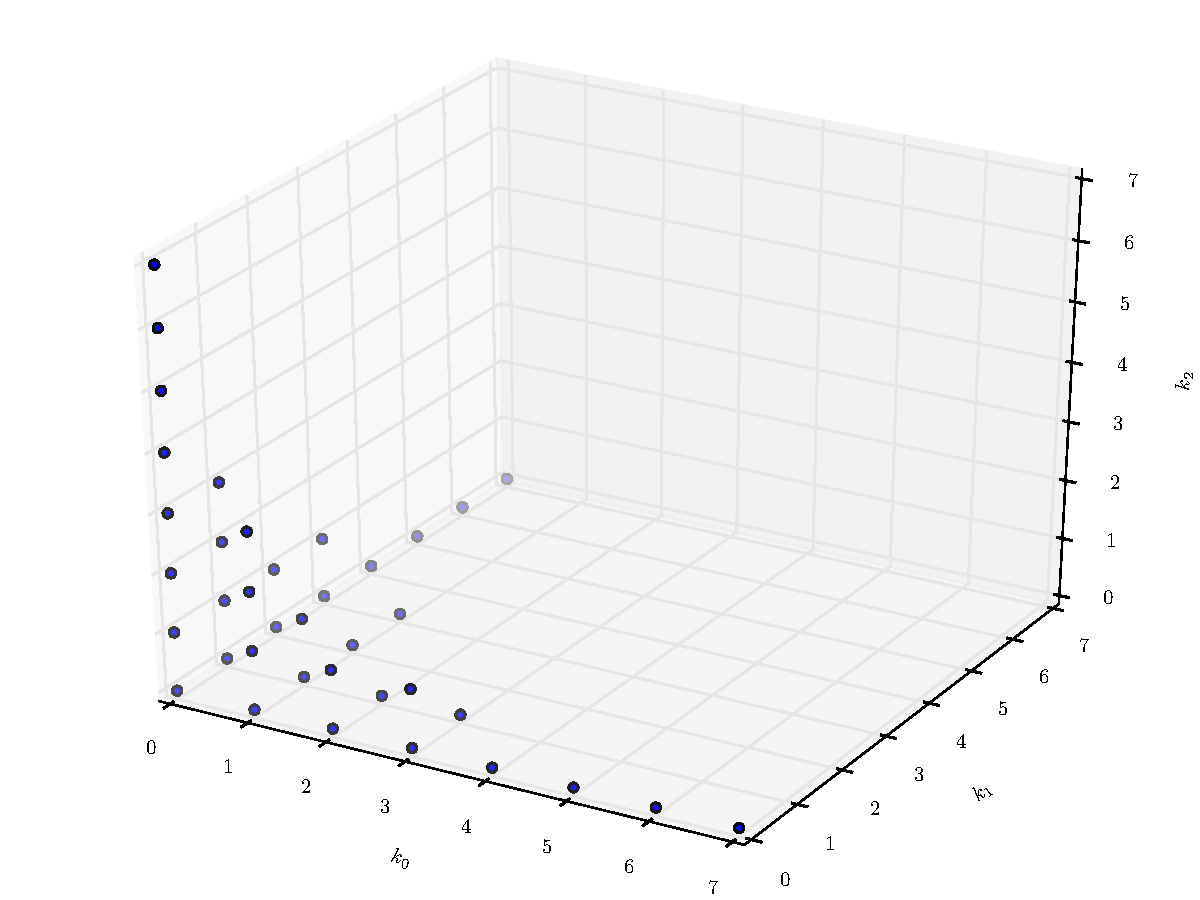
\includegraphics[width=0.5\linewidth]{./fig/hyperbolic_shape_3_8.pdf}
  }
  \subfloat[][]{
    \label{fig:hyperbolic_cut_3_32}
    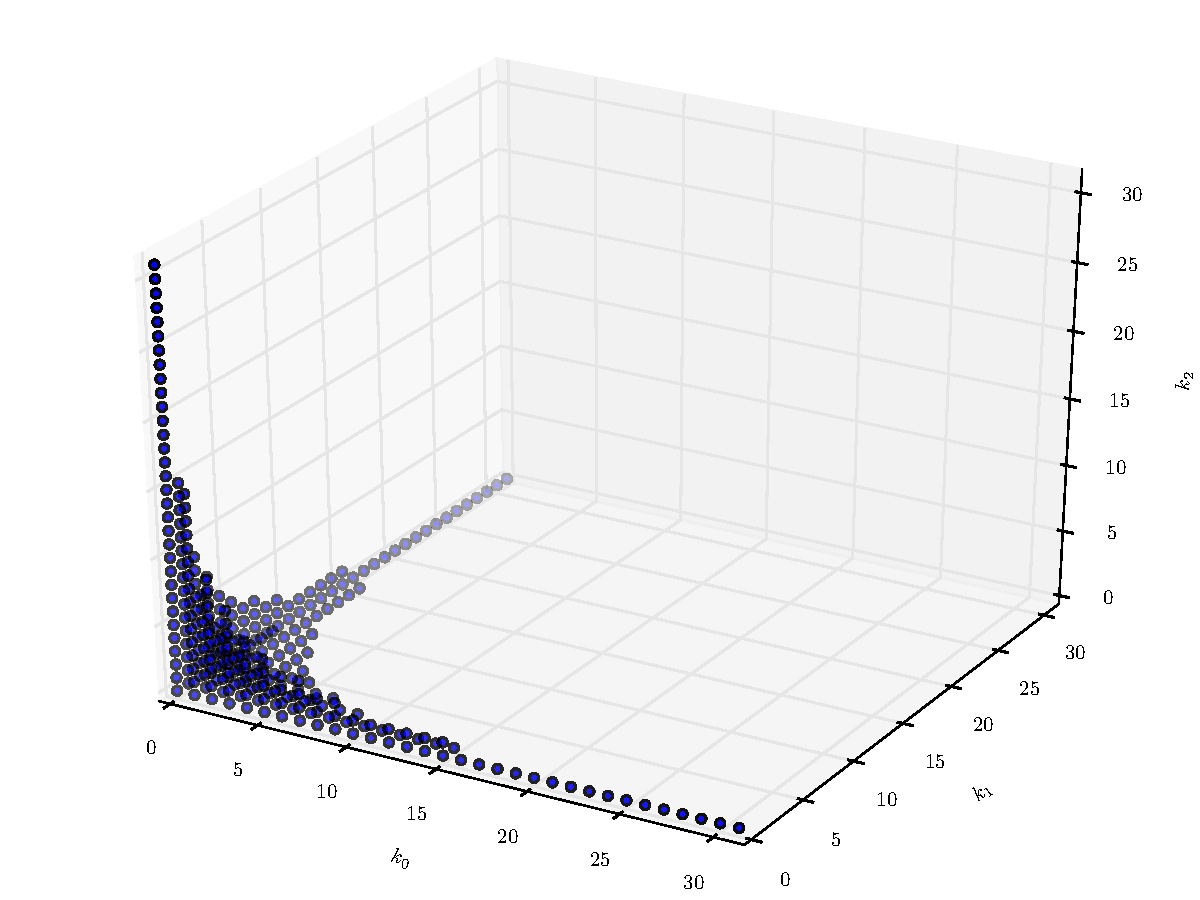
\includegraphics[width=0.5\linewidth]{./fig/hyperbolic_shape_3_32.pdf}
  } \\
  \caption[Hyperbolic cut basis shape in three dimensions]{
    The lattice nodes that are part of a three-dimensional hyperbolic cut basis
    shape. Compared to the full hypercubic basis shape the sparsity of this
    type of basis shape becomes clearly visible.
    \subref{fig:hyperbolic_cut_3_8} $K = 8$
    \subref{fig:hyperbolic_cut_3_32} $K = 32$
    \label{fig:hyperbolic_cut_3D}
  }
\end{figure}

As we see in figures \ref{fig:hyperbolic_cut_2D} and \ref{fig:hyperbolic_cut_3D}
this basis shape has long tails consisting of functions with high frequencies
in one direction. Sometimes we do not need these tails. We can combine the two
basis shapes introduced and define a new shape:

\begin{definition}[Hyperbolic cut basis shape with limits]
  \begin{equation}
    \mathfrak{K}(K, \vec{L}) \assign \left\{ \vec{k} \in \mathbb{N}_0^D :
                             \prod_{d=0}^{D-1}(1+k_d) \leq K
                             \land k_d < L_d \,\forall\, d \in [0,\ldots,D-1] \right\} \,.
  \end{equation}
\end{definition}

The parameter $K \in \mathbb{N}$ is again the sparsity defining the hyperbolic
cuts. The parameter $\vec{L}$ is a list of $D$ elements with each $L_d \in \mathbb{N}$.
These limits act as sharp upper bounds on the entries of $\vec{k}$. In that way
we can combine the two previous basis shapes. If we choose $L_d \geq K \,\forall\,
d \in [0,\ldots, D-1]$ then we obtain a simple hyperbolic cut basis shape. On the
other hand, if we set $K \geq \prod_{d=0}^{D-1} L_d$ we are back in the full
hypercubic case.

\begin{figure}
  \centering
  \subfloat[][]{
    \label{fig:hyperbolic_limited_2_8}
    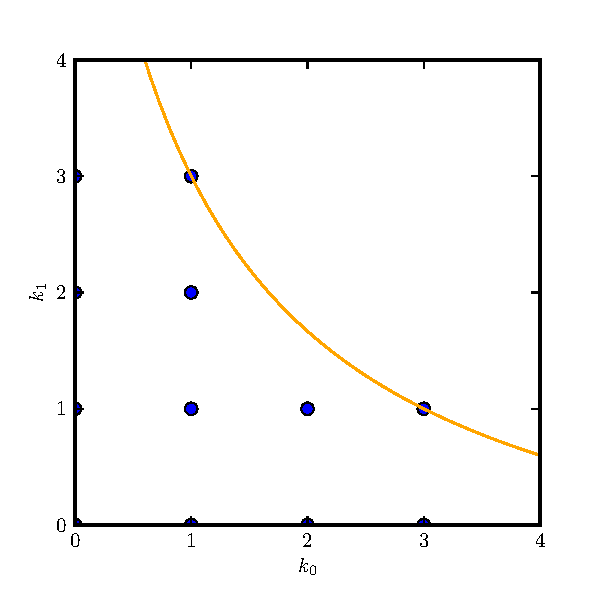
\includegraphics[width=0.5\linewidth]{./fig/hyperbolic_limited_2_8.pdf}
  }
  \subfloat[][]{
    \label{fig:hyperbolic_limited_2_32}
    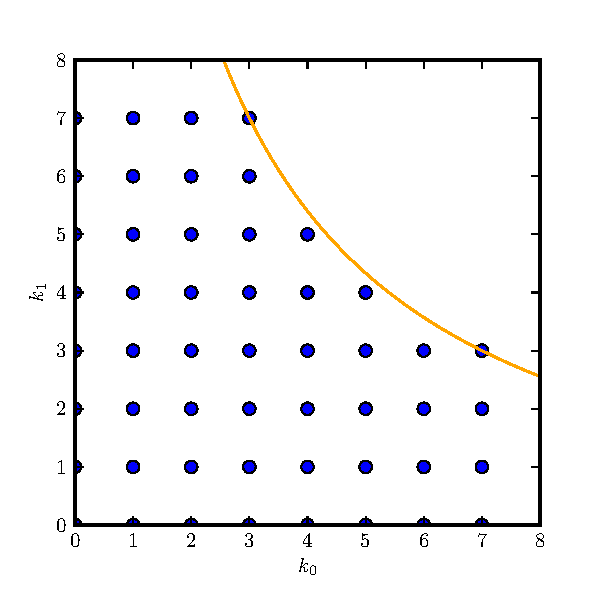
\includegraphics[width=0.5\linewidth]{./fig/hyperbolic_limited_2_32.pdf}
  } \\
  \caption[Hyperbolic cut basis shape with limits in two dimensions]{
    The lattice nodes that are part of a two-dimensional limited hyperbolic cut
    basis shape. Compared to the unlimited hyperbolic cut basis shape
    the long tails are missing here.
    \subref{fig:hyperbolic_limited_2_8} $K = 8$ and $\vec{L} = (4,4)$
    \subref{fig:hyperbolic_limited_2_32} $K = 32$ and $\vec{L} = (8,8)$
    \label{fig:hyperbolic_limited_2D}
  }
\end{figure}

There exist many more possibilities for specific basis shapes. For a generic
basis shape $\mathfrak{K}$ a fundamental property has to hold. We can state
it by the following implication:

\begin{equation}
  \forall\, \vec{k} \in \mathbb{N}_0^D:
  \vec{k} \in \mathfrak{K} \Rightarrow \vec{k} - \vec{e}^d \in \mathfrak{K} \,\forall\, d \in [0, \ldots, D-1] \,.
\end{equation}

% \begin{equation}
%   \mathfrak{K} := \left\{ \vec{k} \in \mathbb{N}_0^D :
%                           \vec{k} - \vec{e}^d \in \mathfrak{K} \,\forall\, d \in [0, \ldots, D-1] \right\} \,.
% \end{equation}

In other words, for each $\vec{k} \in \mathfrak{K}$ it must hold that for all
$d = 0, \ldots, D-1$ the multi-index defined by $k^\prime \assign \vec{k} - \vec{e}^d$
has no negative components and $\vec{k}^\prime \in \mathfrak{K}$. In less formal
terms this means that an index $\vec{k}$ is part of $\mathfrak{K}$ iff all its
backward neighbours are also part of $\mathfrak{K}$. This condition is necessary
for the recursive evaluation of wavepackets which we will show later.

Probably the most general way to write a scalar wavepacket \eqref{eq:scalar_wavepacket}
now is:

\begin{equation}
  \Ket{\Phi} \assign
  \Phi\left[\Pi(t), \mathfrak{K}(t)\right](\vec{x}, t)
  =
  \exp\left(\frac{i S(t)}{\varepsilon^2}\right) \sum_{\vec{k}\in\mathfrak{K}(t)} c_{\vec{k}}(t) \phi_{\vec{k}}\left[\Pi(t)\right](\vec{x})
\end{equation}

which uses an arbitrary, possibly time-adaptive basis shape $\mathfrak{K}(t)$. In
principle we can exchange the basis shapes at each timestep during the simulation.
This provides us with adaptivity for all parameters $\theta$ a basis shape depends on.

Sometimes we will need to bring the elements $\vec{k}$ of a basis shape $\mathfrak{K}$
into a fixed total order. This is done by the \emph{linearisation mapping}.

\begin{definition}[Linearisation mapping]
  A mapping:
  \begin{align*}
    \mu : \mathfrak{K} & \rightarrow \mathbb{N}_0 \\
          \vec{k}      & \mapsto     n
  \end{align*}
  that fixes a total order of the set $\mathfrak{K}$.
\end{definition}

If it is not clear from the context we denote this mapping by $\mu_{\mathfrak{K}}$
to mark explicitly which basis shape it belongs to. In practical cases we usually
have $\mu(\vec{0}) = 0$ but this is not a requirement.

Finally the following two algorithms \ref{al:forward_neighbours} and
\ref{al:backward_neighbours} can be used to find the neighbourhood
of a given multi-index $\vec{k}$ in a general basis shape $\mathfrak{K}$.

\begin{algorithm}
  \caption{Find forward neighbours}
  \label{al:forward_neighbours}
  \begin{algorithmic}
    \REQUIRE The number $D$ of space dimensions
    \REQUIRE The basis shape $\mathfrak{K}$
    \REQUIRE The multi-index $\vec{k}$ whose neighbours we search

    \STATE // List for the result
    \STATE $N \assign \{\}$
    \STATE // Find neighbourhood
    \FOR{$d = 0$ \TO $d = D-1$}
      \STATE $\vec{k}^\prime \assign \vec{k} + \vec{e}^d$
      \IF{$\vec{k}^\prime \in \mathfrak{K}$}
        \STATE $N = N \cup \{(\vec{k}^\prime, d)\}$
      \ENDIF
    \ENDFOR

    \RETURN $N$
  \end{algorithmic}
\end{algorithm}

\begin{algorithm}
  \caption{Find backward neighbours}
  \label{al:backward_neighbours}
  \begin{algorithmic}
    \REQUIRE The number $D$ of space dimensions
    \REQUIRE The basis shape $\mathfrak{K}$
    \REQUIRE The multi-index $\vec{k}$ whose neighbours we search

    \STATE // List for the result
    \STATE $N \assign \{\}$
    \STATE // Find neighbourhood
    \FOR{$d = 0$ \TO $d = D-1$}
      \STATE $\vec{k}^\prime \assign \vec{k} - \vec{e}^d$
      \IF{$\vec{k}^\prime \in \mathfrak{K}$}
        \STATE $N = N \cup \{(\vec{k}^\prime, d)\}$
      \ENDIF
    \ENDFOR

    \RETURN $N$
  \end{algorithmic}
\end{algorithm}


\subsection{Basis shape transformation mappings}


Given two basis shapes $\mathfrak{K}$ and $\mathfrak{K}^\prime$ and their
linearisation mappings:

\begin{align*}
  \mu: \mathfrak{K} & \rightarrow \mathbb{N}_0 \\
  \mu^\prime: \mathfrak{K}^\prime & \rightarrow \mathbb{N}_0 \,.
\end{align*}

We look for a way how to change a data array $\vec{c} \in \mathbb{C}^{|\mathfrak{K}|}$
(storing complex scalar data for each multi-index $\vec{k} \in \mathfrak{K}$
at the position $\vec{c}_{\mu(\vec{k})}$) if we replace the basis shape $\mathfrak{K}$
by $\mathfrak{K}^\prime$. The problem is that the two mappings are in general
incompatible with each other. Hence we have to permute the elements of the array $\vec{c}$.
Referring to figure \ref{fig:map}, the task is now to connect the keys $i$ and
$i^\prime$ such that for all multi-indices $\vec{k} \in \mathfrak{K} \cap \mathfrak{K}^\prime$
it holds that:

\begin{equation*}
  \left(\mu^\prime\right)^{-1} \left( T\left( \mu\left(\vec{k}\right) \right) \right) = \vec{k} \,.
\end{equation*}

The transformation $T$ is bijective if and only if
$\mathfrak{K} \equiv \mathfrak{K} \cap \mathfrak{K}^\prime \equiv \mathfrak{K}^\prime$.

\begin{figure}
  \centering
  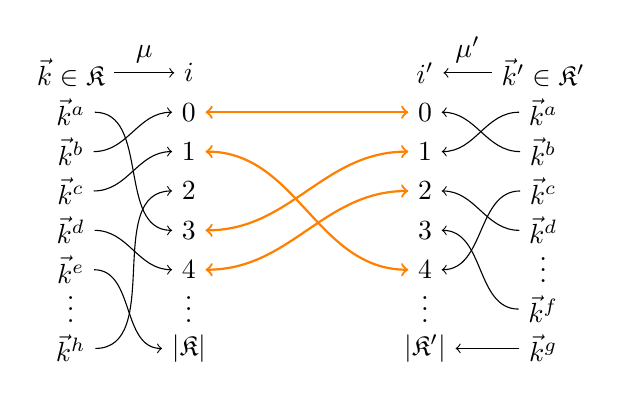
\begin{tikzpicture}[%
    node distance=0.5cm, auto,
    func/.style={scale=0.8,color=gray},
    zero/.style={scale=0.8,color=gray}]

    \node (ko) {$\vec{k} \in \mathfrak{K}$};
    \node (io) [right of=ko, node distance=1.5cm] {$i$};
    \draw[->] (ko) to node {$\mu$} (io);

    \node (ko0) [below of=ko] {$\vec{k}^a$};
    \node (ko1) [below of=ko0] {$\vec{k}^b$};
    \node (ko2) [below of=ko1] {$\vec{k}^c$};
    \node (ko3) [below of=ko2] {$\vec{k}^d$};
    \node (ko4) [below of=ko3] {$\vec{k}^e$};
    \node (ko5) [below of=ko4, node distance=4mm] {$\vdots$};
    \node (ko6) [below of=ko5, node distance=6mm] {$\vec{k}^h$};

    \node (io0) [below of=io] {$0$};
    \node (io1) [below of=io0] {$1$};
    \node (io2) [below of=io1] {$2$};
    \node (io3) [below of=io2] {$3$};
    \node (io4) [below of=io3] {$4$};
    \node (io5) [below of=io4, node distance=4mm] {$\vdots$};
    \node (io6) [below of=io5, node distance=6mm] {$|\mathfrak{K}|$};

    \draw[->] (ko0) to[out=0,in=180] node {} (io3);
    \draw[->] (ko1) to[out=0,in=180] node {} (io0);
    \draw[->] (ko2) to[out=0,in=180] node {} (io1);
    \draw[->] (ko3) to[out=0,in=180] node {} (io4);
    \draw[->] (ko4) to[out=0,in=180] node {} (io6);
    \draw[->] (ko6) to[out=0,in=180] node {} (io2);

    \node (ip) [right of=io, node distance=3cm] {$i^\prime$};
    \node (kp) [right of=ip, node distance=1.5cm] {$\vec{k}^\prime \in \mathfrak{K}^\prime$};
    \draw[<-] (ip) to node {$\mu^\prime$} (kp);

    \node (kp0) [below of=kp] {$\vec{k}^a$};
    \node (kp1) [below of=kp0] {$\vec{k}^b$};
    \node (kp2) [below of=kp1] {$\vec{k}^c$};
    \node (kp3) [below of=kp2] {$\vec{k}^d$};
    \node (kp4) [below of=kp3, node distance=4mm] {$\vdots$};
    \node (kp5) [below of=kp4, node distance=6mm] {$\vec{k}^f$};
    \node (kp6) [below of=kp5] {$\vec{k}^g$};

    \node (ip0) [below of=ip] {$0$};
    \node (ip1) [below of=ip0] {$1$};
    \node (ip2) [below of=ip1] {$2$};
    \node (ip3) [below of=ip2] {$3$};
    \node (ip4) [below of=ip3] {$4$};
    \node (ip5) [below of=ip4, node distance=4mm] {$\vdots$};
    \node (ip6) [below of=ip5, node distance=6mm] {$|\mathfrak{K}^\prime|$};

    \draw[->] (kp0) to[out=180,in=0] node {} (ip1);
    \draw[->] (kp1) to[out=180,in=0] node {} (ip0);
    \draw[->] (kp2) to[out=180,in=0] node {} (ip4);
    \draw[->] (kp3) to[out=180,in=0] node {} (ip2);
    \draw[->] (kp5) to[out=180,in=0] node {} (ip3);
    \draw[->] (kp6) to[out=180,in=0] node {} (ip6);

    \draw[thick, <->, color=orange] (io0) to[out=0,in=180] node {} (ip0);
    \draw[thick, <->, color=orange] (io1) to[out=0,in=180] node {} (ip4);
    \draw[thick, <->, color=orange] (io3) to[out=0,in=180] node {} (ip1);
    \draw[thick, <->, color=orange] (io4) to[out=0,in=180] node {} (ip2);
\end{tikzpicture}

  \caption[Basis shape transformation mapping]
  {The two mappings $\mu$ and $\mu^\prime$ together with the transformation rule $T$ (orange arrows).}
  \label{fig:map}
\end{figure}

When remapping linearly indexed data vectors $\vec{c}_{\mu\left(\vec{k}\right)}$,
we drop the entries for all $\vec{k} \in \mathfrak{K} \setminus \mathfrak{K}^\prime$
and we fill in zero values for all $\vec{k} \in \mathfrak{K}^\prime \setminus \mathfrak{K}$.
The procedure is shown in algorithm \ref{al:basis_shape_remapping} below.

\begin{algorithm}
  \caption{Transformation of basis shapes and data remapping}
  \label{al:basis_shape_remapping}
  \begin{algorithmic}
    \REQUIRE The old basis shape $\mathfrak{K}$
    \REQUIRE The new basis shape $\mathfrak{K}^\prime$
    \REQUIRE An array $\vec{c}$ of length $|\mathfrak{K}|$ containing arbitrary data
    \STATE // Set up the new array of length $|\mathfrak{K}^\prime|$
    \STATE $\vec{c}^\prime \assign \vec{0} \in \mathbb{C}^{|\mathfrak{K}^\prime|}$
    \STATE // Copy over the data we can keep
    \FOR{$\vec{k} \in \mathfrak{K} \cap \mathfrak{K}^\prime$}
      \STATE // Compute linear mapping of $\vec{k}$ in both basis shapes
      \STATE $i \assign \mu\left(\vec{k}\right)$
      \STATE $j \assign \mu^\prime\left(\vec{k}\right)$
      \STATE // Update the array
      \STATE $\vec{c}^\prime\left[j\right] = \vec{c}\left[i\right]$
    \ENDFOR
  \end{algorithmic}
\end{algorithm}

An example of such a mapping is given in figure \ref{fig:trafo_map}.

\begin{figure}
  \centering
  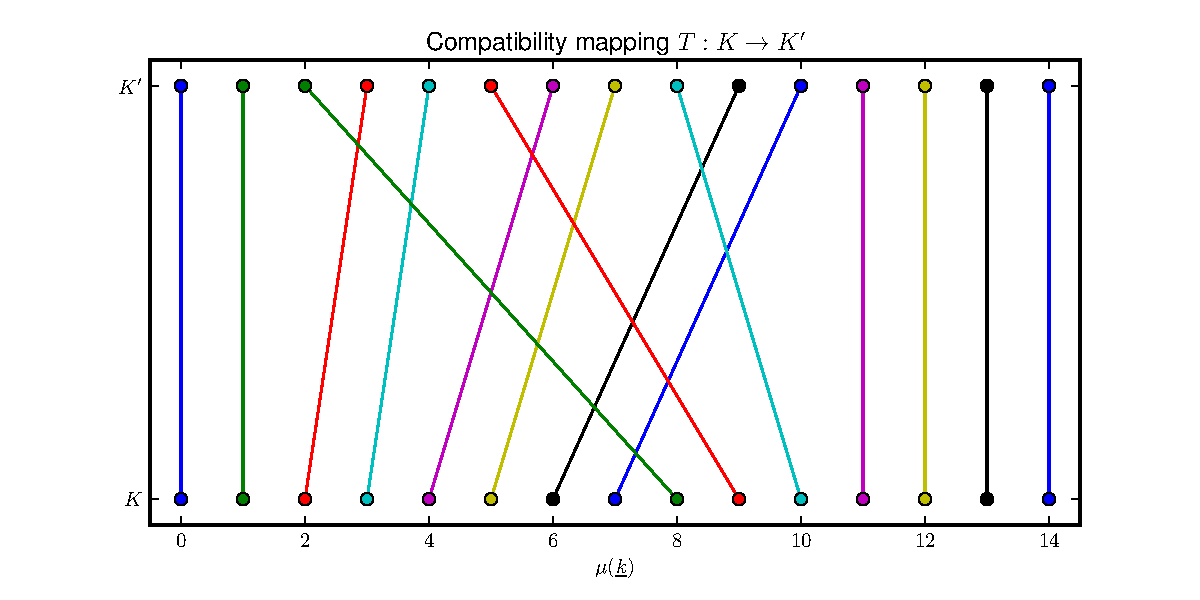
\includegraphics[scale=0.5]{./fig/trafo_map.pdf}
  \caption[Transformation mapping example]
          {An example of a basis shape transformation mapping $T$. The original
          shape was $\mathfrak{K} = \vec{K} = (4,2)$ and $|\mathfrak{K}| = 8$ while
          the new shape is $\mathfrak{K}^{\prime} = \vec{K}^{\prime} = (5,3)$ and
          $|\mathfrak{K}^{\prime}| = 15$.}
  \label{fig:trafo_map}
\end{figure}


\subsection{Basis shape extensions}


For computing the gradients of wavepackets (see section \ref{sec:gradient_computation})
we need to extend the basis shape. Informally spoken, extending a basis shape
means that we add a node in each direction. For each lattice point of a shape
we add all its neighbours. A formal definition is:

\begin{definition}[Basis shape extension]
  Given a basis shape $\mathfrak{K}$ we define its extension $\overline{\mathfrak{K}}$ by:
  \begin{equation*}
    \overline{\mathfrak{K}} \assign \mathfrak{K}
                            \cup \left\{ \vec{k}^\prime : \vec{k}^\prime = \vec{k} + \vec{e}^d \,\forall\, d \in [0,\ldots,D-1]
                                                          \,\forall\, \vec{k} \in \mathfrak{K} \right\} \,.
  \end{equation*}
  This defines the most tight extension. But any even larger basis shape is a
  valid extension too. In any case it holds that $\mathfrak{K} \subset \overline{\mathfrak{K}}$.
\end{definition}

This definition is not handy enough to work with. For some of the less complex basis
shapes $\mathfrak{K}(\theta)$ it is often possible to express the extended shape
$\overline{\mathfrak{K}(\theta^\prime)}$ simply by modifying the parameters
$\theta$ the shape depends on.

If we look at a hypercubic basis shape $\mathfrak{K}(\vec{K})$ then we can express
its extension $\overline{\mathfrak{K}(\vec{K}^\prime)}$ by the new parameters
$\vec{K}^\prime$ which obviously are:

\begin{equation} \label{eq:extend_hypercubic}
  \vec{K}^\prime = [ K_0 + 1, \ldots, K_{D-1} +1 ] \,.
\end{equation}

The attentive reader may notice that in case $D > 1$ this new basis
includes one node too much, namely the lattice point $(K_0, \ldots, K_{D-1})$.
This however poses no problems beside wasting a very small amount of memory.
A basis shape extension has not to be tight with respect to the above definition.

For the hyperbolic cut shape, extension is less trivial. Assume that the sparsity is $K$.
We first look at the extension of a two-dimensional shape. Here the two nodes
$(K-1, 0)$ and $(0, K-1)$ are the outermost ones. Since the whole basis shape is
symmetric under permutation of the axes, we focus only on $(K-1, 0)$ lying on the first
axis. We have to make sure that its neighbours are part of $\overline{\mathfrak{K}}$.
This is guaranteed (by definition \ref{def:hyperbolic_cut_shape}) if we can
construct a new hyperbolic cut shape $\mathfrak{K}^\prime(K^\prime)$ that
contains the node $(K-1,1)$. By using the equation of the above definition we get:

\begin{equation*}
  (1+K-1)(1+1) \leq K^\prime
\end{equation*}

which we can solve for the minimal $K^\prime$ and find that:

\begin{equation} \label{eq:extend_hyperbolic_cut_1D}
  K^\prime = 2 K \,.
\end{equation}

In the general case of $D>1$ dimensions we have a similar equation:

\begin{align*}
  (1+K-1)(1+1)\cdots(1+1) & = (1+K-1)\left(\prod_{d=1}^{D-1}(1+1)\right) \leq K^\prime
\end{align*}

from which we obtain:

\begin{equation} \label{eq:extend_hyperbolic_cut_DD}
  K^\prime = 2^{D-1} K \,.
\end{equation}

This is only valid for $D>1$ and gives for $D=1$ the wrong result $K^\prime = K$.
If we want a single formula valid for all dimensions then we have to start from
the point $\vec{k} = (K, 0, \ldots, 0)$. For this point we get:

\begin{align*}
  (1+K)\left(\prod_{d=1}^{D-1}(1+1)\right) \leq K^\prime
\end{align*}

giving:

\begin{equation} \label{eq:extend_hyperbolic_cut_general}
  K^\prime = 2^{D-1} (K+1) \,.
\end{equation}

However we should note that this leads to overly big extensions for $D>1$
compared to the other formula. For example if we start with a two-dimensional
basis shape with $K=4$ then we get $K^\prime = 8$ and $K^\prime = 10$ respectively.
The basis sizes of the extended shapes are then $20$ and $27$ and the tight extension
given by the direct definition would have size $14$ but is not of hyperbolic
cut type.

Extending a hyperbolic cut basis shape with limits is easy again. First we change
the limits $\vec{L}$ according to \eqref{eq:extend_hypercubic}. Then we increase $K$
by using one of the formulae \eqref{eq:extend_hyperbolic_cut_1D} or
\eqref{eq:extend_hyperbolic_cut_DD} depending on the dimensionality.
That is all we need to do for this type of basis shape.

We can use the limited hyperbolic cut basis shape to produce more tight extensions
of the standard hyperbolic cut basis shapes. For an example, refer to figure
\ref{fig:hyperbolic_extensions_compared}.

\begin{figure}
  \centering
  \subfloat[][]{
    \label{fig:hyperbolic_extension}
    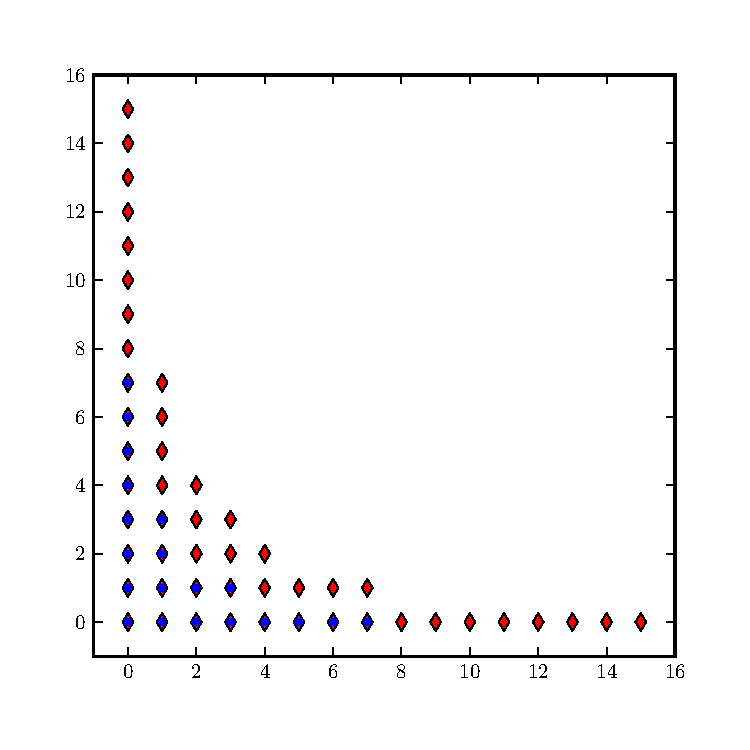
\includegraphics[width=0.5\linewidth]{./fig/hyperbolic_extension.pdf}
  }
  \subfloat[][]{
    \label{fig:hyperbolic_limited}
    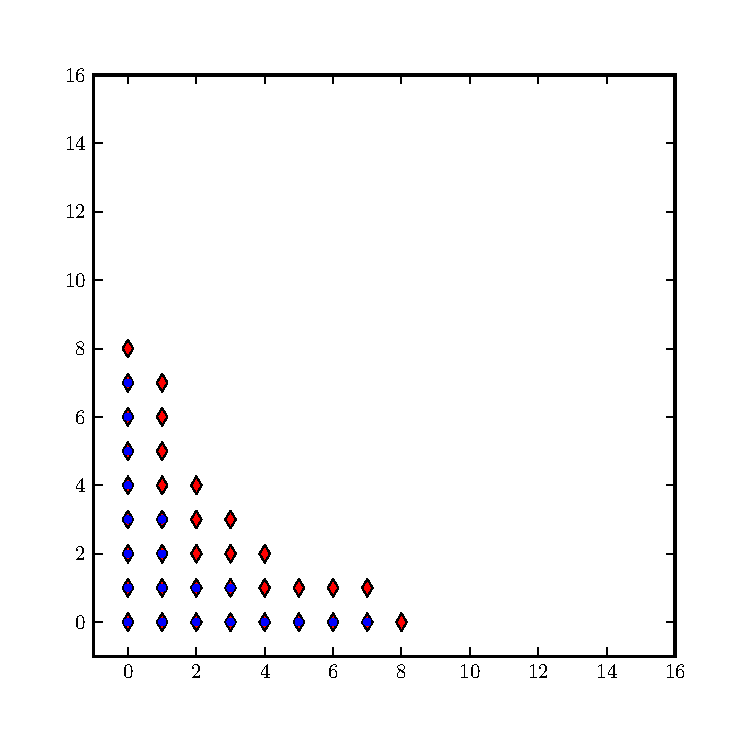
\includegraphics[width=0.5\linewidth]{./fig/hyperbolic_extension_limited.pdf}
  } \\
  \caption[Extensions of a hyperbolic cut basis shape]{
    Comparison of two methods to extend a hyperbolic cut basis shape with $K=8$.
    The original nodes (blue circles) and the nodes of the extension (red diamonds)
    are shown for both methods. The difference in basis size is $14$ nodes.
    \subref{fig:hyperbolic_extension} Extension is again an unlimited hyperbolic
                                      cut shape with $K = 16$.
    \subref{fig:hyperbolic_limited} Extension is a limited hyperbolic cut shape
                                    with $K = 16$ and $\vec{L} = (9,9)$. This extension
                                    introduces only $3$ nodes more than required.
    \label{fig:hyperbolic_extensions_compared}
  }
\end{figure}


\section{Evaluation of wavepackets}


For the numerical simulation we will need to evaluate a wavepacket at sets of
grid nodes $\vec{\gamma} \in \mathbb{R}^D$. The formula for the ground state
\eqref{eq:phi0_Dd} and the recursion \eqref{eq:basis_recursion_DD} for higher
order basis functions is in principle all we need to do this. Even if this
seems to be very simple at first glance there are a few tricky details involved.
In this section we start from the mathematical formulae and work towards an
algorithmic description for computing $\Phi(\vec{\gamma})$.

First we can evaluate the ground state $\phi_{\vec{0}}$ directly by algorithm \ref{al:eval_phi0_DD}.
If this is programmed by using vectorisation for the linear algebra functions we
can even perform the evaluation on a set $\Gamma = \{\gamma_i\}_i$ of nodes simultaneously.
The return value is then not a single scalar value but an array of scalars.
Usually we imagine this to be a row vector of $|\Gamma|$ elements.

\begin{algorithm}
\caption{Evaluate the ground state $\phi_0$ directly}
\label{al:eval_phi0_DD}
\begin{algorithmic}
  \REQUIRE The number $D$ of space dimensions
  \REQUIRE The Hagedorn parameter set $\Pi = \{q,p,Q,P\}$
  \REQUIRE The semi-classical scaling parameter $\varepsilon$
  \REQUIRE The grid node $\vec{\gamma} \in \mathbb{R}^D$

  \STATE // Whether to include the problematic prefactor or not
  \IF{prefactor is True}
    \STATE $\alpha \assign (\pi\varepsilon^2)^{-\frac{D}{4}} (\det\mat{Q})^{-\frac{1}{2}}$
  \ELSE
    \STATE $\alpha \assign (\pi\varepsilon^2)^{-\frac{D}{4}}$
  \ENDIF

  \STATE // The exponent
  \STATE $\vec{u} \assign \vec{\gamma}-\vec{q}$
  \STATE $\beta_1 \assign \dotp{\vec{u}}{\mat{P}\mat{Q}\inv\vec{u}}$
  \STATE $\beta_2 \assign \dotp{\vec{p}}{\vec{u}}$

  \STATE // The full ground state
  \STATE $\phi_{\vec{0}} \assign \alpha \exp\left(\frac{i}{\varepsilon^2}\left(\frac{1}{2}\beta_1 + \beta_2\right)\right)$

  \RETURN $\phi_{\vec{0}}$
\end{algorithmic}
\end{algorithm}

For the higher order basis functions $\phi_{\vec{k}}$ we employ the recursion
formula. With the help of this relation we can compute any $\phi_{\vec{k}}$
given some of the predecessors. For $D=1$ this is easy since we just compute
$\phi_{k+1}$ from $\phi_k$ and $\phi_{k-1}$. In the multi-dimensional case
it is less obvious what happens. To compute the set of all successors $\{\phi_{\vec{k}+\vec{e}^d}\}_{d=0}^{D-1}$
we need the function $\phi_{\vec{k}}$ as well as all antecessors $\{\phi_{\vec{k}-\vec{e}^d}\}_{d=0}^{D-1}$.
We call this rule that specifies how we get new functions from old ones a \emph{stencil}
and denote it by $\mathcal{S}^D$. The figure \ref{fig:recursion_stencils_full}
shows the stencils we get in one, two and three dimensions.

\begin{figure}[h!]
  \centering
  \subfloat[][$\mathcal{S}^1$]{
    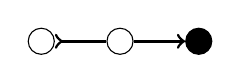
\begin{tikzpicture}[%
  wnode/.style={circle,fill=white,draw},
  bnode/.style={circle,fill=black,draw},
  thickline/.style={line width=1pt}]
  \node[wnode] (O) {};
  \node[wnode] (O1) [left of=O]  {};
  \node[bnode] (N1) [right of=O] {};
  \path[thickline, >-] (O1) edge (O);
  \draw[thickline,->] (O) to node {} (N1);
\end{tikzpicture}

  }
  \subfloat[][$\mathcal{S}^2$]{
    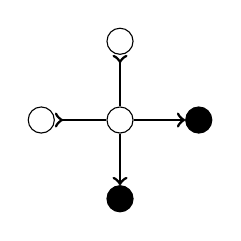
\begin{tikzpicture}[%
  wnode/.style={circle,fill=white,draw},
  bnode/.style={circle,fill=black,draw},
  thickline/.style={line width=1pt}]
  \node[wnode] (O) {};
  \node[wnode] (O1) [left of=O]  {};
  \node[wnode] (O2) [above of=O]  {};
  \node[bnode] (N1) [right of=O] {};
  \node[bnode] (N2) [below of=O] {};
  \path[thickline, >-] (O1) edge (O);
  \path[thickline, >-] (O2) edge (O);
  \draw[thickline,->] (O) to node {} (N1);
  \draw[thickline,->] (O) to node {} (N2);
\end{tikzpicture}

  }
  \subfloat[][$\mathcal{S}^3$]{
    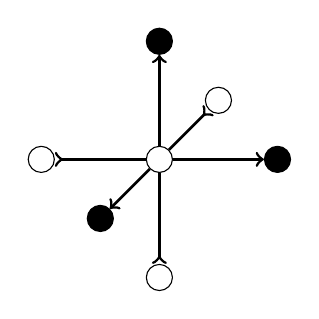
\begin{tikzpicture}[%
  node distance=1.5cm, auto,
  wnode/.style={circle,fill=white,draw},
  bnode/.style={circle,fill=black,draw},
  thickline/.style={line width=1pt}]
  \node[wnode] (O) {};
  \node[wnode] [left of=O] (O1) {};
  \node[wnode] [right of=O, above of=O, node distance=0.75cm] (O2) {};
  \node[wnode] [below of=O] (O3) {};
  \node[bnode] (N1) [right of=O] {};
  \node[bnode] (N2) [left of=O, below of=O, node distance=0.75cm] {};
  \node[bnode] (N3) [above of=O] {};
  \path[thickline, >-] (O1) edge (O);
  \path[thickline, >-] (O2) edge (O);
  \path[thickline, >-] (O3) edge (O);
  \draw[thickline,->] (O) to node {} (N1);
  \draw[thickline,->] (O) to node {} (N2);
  \draw[thickline,->] (O) to node {} (N3);
\end{tikzpicture}

  } \\
    \caption[Full recursion stencils in one, two and three dimensions]{The basis
    function recursion stencils in one, two and three dimensions. The black nodes
    can be computed given the white ones. This works in one single step, i.e.
    we need all white ones and get all black ones.}
    \label{fig:recursion_stencils_full}
\end{figure}

For all these recurrences we need starting points. The only point we know is $\phi_{\vec{0}}$.
But as we found earlier we can insert a $0$ for all $\vec{k}$ where $\exists k_d$ with $k_d < 0$.
Hence we have indeed enough known values to get the process started. An example
of how this works in two dimensions is shown in figure \ref{fig:naive_stencil_application}
and algorithm \ref{al:eval_phik_DD_naive}.

\begin{figure}
  \centering
  \begin{tikzpicture}[%
    func/.style={scale=0.8,color=gray},
    zero/.style={scale=0.8,color=black}]

    \node[zero] (v0m1) at (1,0) {$0$};
    \node[zero] (v1m1) at (2,0) {$0$};
    \node[zero] (v2m1) at (3,0) {$0$};
    \node[zero] (v3m1) at (4,0) {$0$};

    \node[zero] (vm10) at (0,1) {$0$};
    \node[zero] (vm11) at (0,2) {$0$};
    \node[zero] (vm12) at (0,3) {$0$};
    \node[zero] (vm13) at (0,4) {$0$};

    \node[func,color=black] (v00) at (1,1) {$\phi_{0,0}$};

    \node[func,color=blue] (v01) at (1,2) {$\phi_{0,1}$};
    \node[func,color=green] (v02) at (1,3) {$\phi_{0,2}$};
    \node[func] (v03) at (1,4) {$\phi_{0,3}$};

    \node[func,color=blue] (v10) at (2,1) {$\phi_{1,0}$};
    \node[func,color=green] (v11) at (2,2) {$\phi_{1,1}$};
    \node[func] (v12) at (2,3) {$\phi_{1,2}$};
    \node[func] (v13) at (2,4) {$\phi_{1,3}$};

    \node[func,color=green] (v20) at (3,1) {$\phi_{2,0}$};
    \node[func] (v21) at (3,2) {$\phi_{2,1}$};
    \node[func] (v22) at (3,3) {$\phi_{2,2}$};
    \node[func] (v23) at (3,4) {$\phi_{2,3}$};

    \node[func] (v30) at (4,1) {$\phi_{3,0}$};
    \node[func] (v31) at (4,2) {$\phi_{3,1}$};
    \node[func] (v32) at (4,3) {$\phi_{3,2}$};
    \node[func] (v33) at (4,4) {$\phi_{3,3}$};

    \begin{scope}
    \draw[draw=green!80,line width=0.8pt] ($(v10)+(0.0,0.3)$)
        to[out=190,in=350] ($(v00)+(0.0,0.3)$)
        to[out=170,in=90] ($(v00)+(-0.3,0.0)$)
        to[out=270,in=190] ($(v00)+(0.0,-0.3)$)
        to[out=10,in=80] ($(v1m1)+(-0.2,0.0)$)
        to[out=260,in=180] ($(v1m1)+(0.0,-0.2)$)
        to[out=0,in=280] ($(v1m1)+(0.2,0.0)$)
        to[out=100,in=260] ($(v10)+(0.3,0.0)$)
        to[out=80,in=10] ($(v10)+(0.0,0.3)$);
    \draw[draw=green!80,->,line width=0.8pt] ($(v10)+(0.0,0.3)$) -- (v11);
    \draw[draw=green!80,->,line width=0.8pt] ($(v10)+(0.3,0.0)$) -- (v20);
    \end{scope}

    \begin{scope}
    \draw[draw=green!80,line width=0.8pt] ($(v01)+(0.0,0.3)$)
        to[out=190,in=350] ($(vm11)+(0.0,0.2)$)
        to[out=170,in=90] ($(vm11)+(-0.2,0.0)$)
        to[out=270,in=190] ($(vm11)+(0.0,-0.2)$)
        to[out=10,in=80] ($(v00)+(-0.3,0.0)$)
        to[out=260,in=180] ($(v00)+(0.0,-0.3)$)
        to[out=0,in=280] ($(v00)+(0.3,0.0)$)
        to[out=100,in=260] ($(v01)+(0.3,0.0)$)
        to[out=80,in=10] ($(v01)+(0.0,0.3)$);
    \draw[draw=green!80,->,line width=0.8pt] ($(v01)+(0.0,0.3)$) -- (v02);
    \draw[draw=green!80,->,line width=0.8pt] ($(v01)+(0.3,0.0)$) -- (v11);
    \end{scope}

    \begin{scope}
    \draw[draw=blue!100,line width=0.8pt] ($(v00)+(0.0,0.3)$)
        to[out=190,in=350] ($(vm10)+(0.0,0.2)$)
        to[out=170,in=90] ($(vm10)+(-0.2,0.0)$)
        to[out=270,in=190] ($(vm10)+(0.0,-0.2)$)
        to[out=10,in=80] ($(v0m1)+(-0.2,0.0)$)
        to[out=260,in=180] ($(v0m1)+(0.0,-0.2)$)
        to[out=0,in=280] ($(v0m1)+(0.2,0.0)$)
        to[out=100,in=260] ($(v00)+(0.3,0.0)$)
        to[out=80,in=10] ($(v00)+(0.0,0.3)$);
    \draw[draw=blue,->,line width=0.8pt] ($(v00)+(0.0,0.3)$) -- (v01);
    \draw[draw=blue,->,line width=0.8pt] ($(v00)+(0.3,0.0)$) -- (v10);
    \end{scope}
\end{tikzpicture}

  \caption[Naive stencil application in two dimensions]{Naive stencil application
           in two dimensions. All values we initially know are printed in black.
           In a first step we centre the stencil $\mathcal{S}^2$ at the node
           $\vec{k} = (0,0)$ (blue) and compute $\phi_{0,1}$ and $\phi_{1,0}$.
           Next we can apply the stencil there (green) and find $\phi_{0,2}$,
           $\phi_{1,1}$ and $\phi_{2,0}$.}
  \label{fig:naive_stencil_application}
\end{figure}

\begin{algorithm}
  \caption{Evaluate higher order states $\phi_k$ recursively (naive version)}
  \label{al:eval_phik_DD_naive}
  \begin{algorithmic}
    \REQUIRE The number $D$ of space dimensions
    \REQUIRE The Hagedorn parameter set $\Pi = \{q,p,Q,P\}$
    \REQUIRE The semi-classical scaling parameter $\varepsilon$
    \REQUIRE The basis shape $\mathfrak{K}$ and its linearisation mapping $\mu$
    \REQUIRE The grid node $\vec{\gamma} \in \mathbb{R}^D$

    \STATE // Storage space for the result
    \STATE $\vec{\psi} \assign \vec{0} \in \mathbb{C}^{|\mathfrak{K}|}$

    \STATE // Evaluate the ground state by algorithm \ref{al:eval_phi0_DD}
    \STATE $\vec{\psi}[\mu(\vec{0})] = \text{\bf{evaluate\_ground\_state}}(D, \Pi, \varepsilon, \vec{\gamma})$

    \STATE // Loop over the multi-indices
    \FOR{$\vec{k} \in \mathfrak{K}$}
      \STATE // Backward neighbours
      \STATE $\vec{\xi} \assign \vec{0} \in \mathbb{C}^{D}$
      \FOR{$d = 0$ \TO $d = D-1$}
        \STATE $\vec{k}^\prime \assign \vec{k} - \vec{e}^{d}$
        \IF{$\vec{k}^\prime \in \mathfrak{K}$}
          \STATE $\vec{\xi}[d] = \sqrt{\vec{k}[d]} \, \vec{\psi}[\mu(\vec{k}^\prime)]$
        \ENDIF
      \ENDFOR

      \STATE // Compute 3-term recursion
      \STATE $\vec{\alpha} \assign (\vec{\gamma} - \vec{q}) \, \vec{\psi}[\mu(\vec{k})]$
      \STATE $\vec{\beta_1} \assign \sqrt{\frac{2}{\varepsilon^2}} \, \mat{Q}\inv \cdot \vec{\alpha}$
      \STATE $\vec{\beta_2} \assign \mat{Q}\inv \conj{\mat{Q}} \cdot \vec{\xi}$
      \STATE $\vec{\beta} \assign \vec{\beta_1} - \vec{\beta_2}$

      \STATE // Store the results at the correct positions (forward neighbours)
      \FOR{$d = 0$ \TO $d = D-1$}
        \STATE $\vec{k}^\prime \assign \vec{k} + \vec{e}^d$
        \IF{$\vec{k}^\prime \in \mathfrak{K}$}
          \STATE $\vec{\psi}[\mu(\vec{k}^\prime)] = \frac{\vec{\beta}[d]}{\sqrt{\vec{k}[d] + 1}}$
        \ENDIF
      \ENDFOR
  \ENDFOR

  \STATE // Whether to include the problematic prefactor or not
  \STATE // Make sure not to divide twice for $\phi_{\vec{0}}$!
  \IF{prefactor is True}
    \STATE $\vec{\psi} = \frac{1}{\sqrt{\det\mat{Q}}} \, \vec{\psi}$
  \ENDIF

  \RETURN $\vec{\psi}$
\end{algorithmic}
\end{algorithm}

The most severe issue with this naive stencil application is that we compute almost
all functions twice, here this becomes obvious the first time for $\phi_{1,1}$.
Even worse, in $D$ dimensions we would compute almost all functions $D$ times!

Therefore we seek a better way to organise the computations. To achieve this goal we
modify the stencil in a way that seems to be counter intuitive at first. Define the
modified \emph{cheap stencil} as follows.

\begin{definition}[Cheap recursion stencil]
  The cheap recursion stencil does not compute all $D$ outputs $\phi_{\vec{k}+\vec{e}^d}$
  for all $d \in [0, \ldots, D-1]$ but only one output for a single and fixed direction $d$.
  We denote the cheap stencil for direction $d$ and in $D$ dimensions by $\mathcal{S}_d^D$.
  In $D$ dimensions we have $D$ different stencils:
  \begin{equation*}
    \mathcal{S}^D_d \quad d \in [0, \ldots, D-1] \, .
  \end{equation*}
\end{definition}

Figures \ref{fig:recursion_stencils_cheap_2D} and \ref{fig:recursion_stencils_cheap_3D}
give an impression how the stencils look like and how they work in two and three
dimensions. In one dimension we obviously find $\mathcal{S}^1_0 \equiv \mathcal{S}^1$.
In all dimensions it holds that we recover the full stencil $\mathcal{S}^D$ as the sum:

\begin{equation*}
  \mathcal{S}^D = \bigoplus_{d=0}^{D-1} \mathcal{S}^D_d
\end{equation*}

where all stencils are applied centred at the very same node $\phi_{\vec{k}}$.

\begin{figure}[h!]
  \centering
  \subfloat[][$\mathcal{S}^2_0$]{
    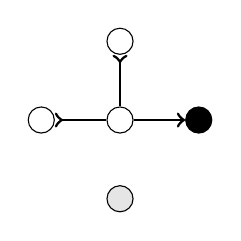
\begin{tikzpicture}[%
  wnode/.style={circle,fill=white,draw},
  bnode/.style={circle,fill=black,draw},
  gnode/.style={circle,fill=black!10,draw},
  thickline/.style={line width=1pt}]
  \node[wnode] (O) {};
  \node[wnode] (O1) [left of=O]  {};
  \node[wnode] (O2) [above of=O]  {};
  \node[bnode] (N1) [right of=O] {};
  \node[gnode] (N2) [below of=O] {};
  \path[thickline, >-] (O1) edge (O);
  \path[thickline, >-] (O2) edge (O);
  \draw[thickline,->] (O) to node {} (N1);
\end{tikzpicture}

  }
  \subfloat[][$\mathcal{S}^2_1$]{
    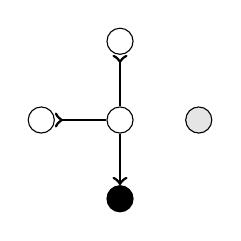
\begin{tikzpicture}[%
  wnode/.style={circle,fill=white,draw},
  bnode/.style={circle,fill=black,draw},
  gnode/.style={circle,fill=black!10,draw},
  thickline/.style={line width=1pt}]
  \node[wnode] (O) {};
  \node[wnode] (O1) [left of=O]  {};
  \node[wnode] (O2) [above of=O]  {};
  \node[gnode] (N1) [right of=O] {};
  \node[bnode] (N2) [below of=O] {};
  \path[thickline, >-] (O1) edge (O);
  \path[thickline, >-] (O2) edge (O);
  \draw[thickline,->] (O) to node {} (N2);
\end{tikzpicture}

  } \\
    \caption[Cheap recursion stencils in two dimensions]{The modified basis
    function recursion stencils $\mathcal{S}^2_d$ in two dimensions.
    The black node can be computed given the white nodes. The grey node would be
    computed by the full stencil $\mathcal{S}^2$ but is intentionally left out by
    the modified ones.}
    \label{fig:recursion_stencils_cheap_2D}
\end{figure}

\begin{figure}[h!]
  \centering
  \subfloat[][$\mathcal{S}^3_0$]{
    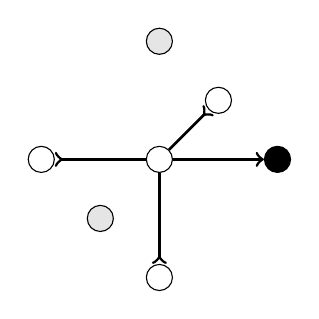
\begin{tikzpicture}[%
  node distance=1.5cm, auto,
  wnode/.style={circle,fill=white,draw},
  bnode/.style={circle,fill=black,draw},
  gnode/.style={circle,fill=black!10,draw},
  thickline/.style={line width=1pt}]
  \node[wnode] (O) {};
  \node[wnode] [left of=O] (O1) {};
  \node[wnode] [right of=O, above of=O, node distance=0.75cm] (O2) {};
  \node[wnode] [below of=O] (O3) {};
  \node[bnode] (N1) [right of=O] {};
  \node[gnode] (N2) [left of=O, below of=O, node distance=0.75cm] {};
  \node[gnode] (N3) [above of=O] {};
  \path[thickline, >-] (O1) edge (O);
  \path[thickline, >-] (O2) edge (O);
  \path[thickline, >-] (O3) edge (O);
  \draw[thickline,->] (O) to node {} (N1);
\end{tikzpicture}

  }
  \subfloat[][$\mathcal{S}^3_1$]{
    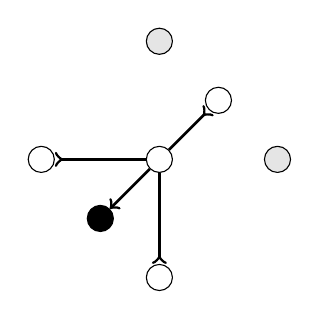
\begin{tikzpicture}[%
  node distance=1.5cm, auto,
  wnode/.style={circle,fill=white,draw},
  bnode/.style={circle,fill=black,draw},
  gnode/.style={circle,fill=black!10,draw},
  thickline/.style={line width=1pt}]
  \node[wnode] (O) {};
  \node[wnode] [left of=O] (O1) {};
  \node[wnode] [right of=O, above of=O, node distance=0.75cm] (O2) {};
  \node[wnode] [below of=O] (O3) {};
  \node[gnode] (N1) [right of=O] {};
  \node[bnode] (N2) [left of=O, below of=O, node distance=0.75cm] {};
  \node[gnode] (N3) [above of=O] {};
  \path[thickline, >-] (O1) edge (O);
  \path[thickline, >-] (O2) edge (O);
  \path[thickline, >-] (O3) edge (O);
  \draw[thickline,->] (O) to node {} (N2);
\end{tikzpicture}

  }
  \subfloat[][$\mathcal{S}^3_2$]{
    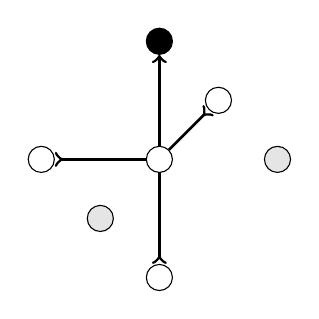
\begin{tikzpicture}[%
  node distance=1.5cm, auto,
  wnode/.style={circle,fill=white,draw},
  bnode/.style={circle,fill=black,draw},
  gnode/.style={circle,fill=black!10,draw},
  thickline/.style={line width=1pt}]
  \node[wnode] (O) {};
  \node[wnode] [left of=O] (O1) {};
  \node[wnode] [right of=O, above of=O, node distance=0.75cm] (O2) {};
  \node[wnode] [below of=O] (O3) {};
  \node[gnode] (N1) [right of=O] {};
  \node[gnode] (N2) [left of=O, below of=O, node distance=0.75cm] {};
  \node[bnode] (N3) [above of=O] {};
  \path[thickline, >-] (O1) edge (O);
  \path[thickline, >-] (O2) edge (O);
  \path[thickline, >-] (O3) edge (O);
  \draw[thickline,->] (O) to node {} (N3);
\end{tikzpicture}

  } \\
    \caption[Cheap recursion stencils in three dimensions]{The modified basis
    function recursion stencils $\mathcal{S}^3_d$ in three dimensions.
    The black node can be computed given the white nodes. The grey nodes would be
    computed by the full stencil $\mathcal{S}^3$ but is intentionally left out by
    the modified ones.}
    \label{fig:recursion_stencils_cheap_3D}
\end{figure}

Formally we have just used the $d$-th row of equation \eqref{eq:basis_recursion_DD} only
to compute the application of $\mathcal{S}^D_d$ to $\phi_{\vec{k}}$. By using colon or
slicing notation we can write the formula for the modified stencils $\mathcal{S}^D_d$
as follows:

\begin{equation}
  \sqrt{k_d +1} \phi_{k + e_d}
  = \sqrt{\frac{2}{\varepsilon^2}}
  \left(Q^{-1}\right)_{d,:}
  \left( x-q \right)
  \phi_{k}
  -
  \left(Q^{-1} \overline{Q} \right)_{d,:}
  \begin{pmatrix}
    \sqrt{k_0} \phi_{k - e_0} \\
    \vdots \\
    \sqrt{k_{D-1}} \phi_{k - e_{D-1}}
  \end{pmatrix} \,.
\end{equation}

What can we do with these modified stencils? And why should they be more efficient?
The most important gain is that we do never compute any function twice. But for this
we have to use the new stencils in a clever way. We start with an empty grid like the
one in figure \ref{fig:naive_stencil_application}. It contains only the ground state
evaluated $\phi_{\vec{0}}$. Now we apply the stencil $\mathcal{S}^D_0$ along the first
direction $d=0$ until we overflow. This works fine as we use the ground state as
anchor point for this \emph{recursion chain} and produce new anchor points successively.
This process is shown in figure \ref{fig:efficient_stencil_application_d0}.

\begin{figure}
  \centering
  \begin{tikzpicture}[%
    func/.style={scale=0.8,color=gray},
    zero/.style={scale=0.8,color=black}]

    \node[zero] (v0m1) at (1,0) {$0$};
    \node[zero] (v1m1) at (2,0) {$0$};
    \node[zero] (v2m1) at (3,0) {$0$};
    \node[zero] (v3m1) at (4,0) {$0$};

    \node[zero] (vm10) at (0,1) {$0$};
    \node[zero] (vm11) at (0,2) {$0$};
    \node[zero] (vm12) at (0,3) {$0$};
    \node[zero] (vm13) at (0,4) {$0$};

    \node[func,color=black] (v00) at (1,1) {$\phi_{0,0}$};

    \node[func] (v01) at (1,2) {$\phi_{0,1}$};
    \node[func] (v02) at (1,3) {$\phi_{0,2}$};
    \node[func] (v03) at (1,4) {$\phi_{0,3}$};

    \node[func,color=blue] (v10) at (2,1) {$\phi_{1,0}$};
    \node[func] (v11) at (2,2) {$\phi_{1,1}$};
    \node[func] (v12) at (2,3) {$\phi_{1,2}$};
    \node[func] (v13) at (2,4) {$\phi_{1,3}$};

    \node[func,color=blue] (v20) at (3,1) {$\phi_{2,0}$};
    \node[func] (v21) at (3,2) {$\phi_{2,1}$};
    \node[func] (v22) at (3,3) {$\phi_{2,2}$};
    \node[func] (v23) at (3,4) {$\phi_{2,3}$};

    \node[func,color=blue] (v30) at (4,1) {$\phi_{3,0}$};
    \node[func] (v31) at (4,2) {$\phi_{3,1}$};
    \node[func] (v32) at (4,3) {$\phi_{3,2}$};
    \node[func] (v33) at (4,4) {$\phi_{3,3}$};

    \begin{scope}
    \draw[draw=blue!60,line width=0.8pt] ($(v20)+(0.0,0.3)$)
        to[out=190,in=350] ($(v10)+(0.0,0.3)$)
        to[out=170,in=90] ($(v10)+(-0.3,0.0)$)
        to[out=270,in=190] ($(v10)+(0.0,-0.3)$)
        to[out=10,in=80] ($(v2m1)+(-0.2,0.0)$)
        to[out=260,in=180] ($(v2m1)+(0.0,-0.2)$)
        to[out=0,in=280] ($(v2m1)+(0.2,0.0)$)
        to[out=100,in=260] ($(v20)+(0.3,0.0)$)
        to[out=80,in=10] ($(v20)+(0.0,0.3)$);
    \draw[draw=blue!60,->,line width=0.8pt] ($(v20)+(0.3,0.0)$) -- (v30);
    \end{scope}

    \begin{scope}
    \draw[draw=blue!80,line width=0.8pt] ($(v10)+(0.0,0.3)$)
        to[out=190,in=350] ($(v00)+(0.0,0.3)$)
        to[out=170,in=90] ($(v00)+(-0.3,0.0)$)
        to[out=270,in=190] ($(v00)+(0.0,-0.3)$)
        to[out=10,in=80] ($(v1m1)+(-0.2,0.0)$)
        to[out=260,in=180] ($(v1m1)+(0.0,-0.2)$)
        to[out=0,in=280] ($(v1m1)+(0.2,0.0)$)
        to[out=100,in=260] ($(v10)+(0.3,0.0)$)
        to[out=80,in=10] ($(v10)+(0.0,0.3)$);
    \draw[draw=blue!80,->,line width=0.8pt] ($(v10)+(0.3,0.0)$) -- (v20);
    \end{scope}

    \begin{scope}
    \draw[draw=blue!100,line width=0.8pt] ($(v00)+(0.0,0.3)$)
        to[out=190,in=350] ($(vm10)+(0.0,0.2)$)
        to[out=170,in=90] ($(vm10)+(-0.2,0.0)$)
        to[out=270,in=190] ($(vm10)+(0.0,-0.2)$)
        to[out=10,in=80] ($(v0m1)+(-0.2,0.0)$)
        to[out=260,in=180] ($(v0m1)+(0.0,-0.2)$)
        to[out=0,in=280] ($(v0m1)+(0.2,0.0)$)
        to[out=100,in=260] ($(v00)+(0.3,0.0)$)
        to[out=80,in=10] ($(v00)+(0.0,0.3)$);
    \draw[draw=blue,->,line width=0.8pt] ($(v00)+(0.3,0.0)$) -- (v10);
    \end{scope}
\end{tikzpicture}

  \caption[Efficient stencil application in two dimensions]{
           First step in the efficient application of the recursion stencils
           in two dimensions. All values we initially know are printed in black.
           In a first step we centre the cheap stencil $\mathcal{S}^2_0$ at the
           node $\vec{k} = (0,0)$ and compute $\phi_{1,0}$ only. Next we can use
           the same stencil centred at $\phi_{1,0}$ and find $\phi_{2,0}$. We
           continue like this until an overflow occurs. (In this little example
           we are done after the next step.)}
  \label{fig:efficient_stencil_application_d0}
\end{figure}

After this first step we can not apply the stencil $\mathcal{S}^2_0$ anymore.
There is no anchor point left that would give us new nodes in the lattice.
But we have build a whole chain $\phi_{k, 0}$ of starting points. Hence we take
the stencil $\mathcal{S}^2_1$ at hand and go along the second direction $d=1$
starting a chain for each $\phi_{k,0}$. Again we follow each chain until an
overflow occurs. Note that we must do this in increasing order of the index $k$
because we need the values to the left of where we centre $\mathcal{S}^2_1$.
Figure \ref{fig:efficient_stencil_application_d1} shows the process for the
first two chains starting at $\phi_{0,0}$ and $\phi_{1,0}$.

\begin{figure}[h!]
  \centering
  \subfloat[][]{
    \begin{tikzpicture}[%
    func/.style={scale=0.8,color=gray},
    zero/.style={scale=0.8,color=black}]

    \node[zero] (v0m1) at (1,0) {$0$};
    \node[zero] (v1m1) at (2,0) {$0$};
    \node[zero] (v2m1) at (3,0) {$0$};
    \node[zero] (v3m1) at (4,0) {$0$};

    \node[zero] (vm10) at (0,1) {$0$};
    \node[zero] (vm11) at (0,2) {$0$};
    \node[zero] (vm12) at (0,3) {$0$};
    \node[zero] (vm13) at (0,4) {$0$};

    \node[func,color=black] (v00) at (1,1) {$\phi_{0,0}$};

    \node[func,color=green] (v01) at (1,2) {$\phi_{0,1}$};
    \node[func,color=green] (v02) at (1,3) {$\phi_{0,2}$};
    \node[func,color=green] (v03) at (1,4) {$\phi_{0,3}$};

    \node[func,color=black] (v10) at (2,1) {$\phi_{1,0}$};
    \node[func] (v11) at (2,2) {$\phi_{1,1}$};
    \node[func] (v12) at (2,3) {$\phi_{1,2}$};
    \node[func] (v13) at (2,4) {$\phi_{1,3}$};

    \node[func,color=black] (v20) at (3,1) {$\phi_{2,0}$};
    \node[func] (v21) at (3,2) {$\phi_{2,1}$};
    \node[func] (v22) at (3,3) {$\phi_{2,2}$};
    \node[func] (v23) at (3,4) {$\phi_{2,3}$};

    \node[func,color=black] (v30) at (4,1) {$\phi_{3,0}$};
    \node[func] (v31) at (4,2) {$\phi_{3,1}$};
    \node[func] (v32) at (4,3) {$\phi_{3,2}$};
    \node[func] (v33) at (4,4) {$\phi_{3,3}$};

    \begin{scope}
    \draw[draw=green!60,line width=0.8pt] ($(v02)+(0.0,0.3)$)
        to[out=190,in=350] ($(vm12)+(0.0,0.2)$)
        to[out=170,in=90] ($(vm12)+(-0.2,0.0)$)
        to[out=270,in=190] ($(vm12)+(0.0,-0.2)$)
        to[out=10,in=80] ($(v01)+(-0.3,0.0)$)
        to[out=260,in=180] ($(v01)+(0.0,-0.3)$)
        to[out=0,in=280] ($(v01)+(0.3,0.0)$)
        to[out=100,in=260] ($(v02)+(0.3,0.0)$)
        to[out=80,in=10] ($(v02)+(0.0,0.3)$);
    \draw[draw=green!60,->,line width=0.8pt] ($(v02)+(0.0,0.3)$) -- (v03);
    \end{scope}

    \begin{scope}
    \draw[draw=green!80,line width=0.8pt] ($(v01)+(0.0,0.3)$)
        to[out=190,in=350] ($(vm11)+(0.0,0.2)$)
        to[out=170,in=90] ($(vm11)+(-0.2,0.0)$)
        to[out=270,in=190] ($(vm11)+(0.0,-0.2)$)
        to[out=10,in=80] ($(v00)+(-0.3,0.0)$)
        to[out=260,in=180] ($(v00)+(0.0,-0.3)$)
        to[out=0,in=280] ($(v00)+(0.3,0.0)$)
        to[out=100,in=260] ($(v01)+(0.3,0.0)$)
        to[out=80,in=10] ($(v01)+(0.0,0.3)$);
    \draw[draw=green!80,->,line width=0.8pt] ($(v01)+(0.0,0.3)$) -- (v02);
    \end{scope}

    \begin{scope}
    \draw[draw=green!100,line width=0.8pt] ($(v00)+(0.0,0.3)$)
        to[out=190,in=350] ($(vm10)+(0.0,0.2)$)
        to[out=170,in=90] ($(vm10)+(-0.2,0.0)$)
        to[out=270,in=190] ($(vm10)+(0.0,-0.2)$)
        to[out=10,in=80] ($(v0m1)+(-0.2,0.0)$)
        to[out=260,in=180] ($(v0m1)+(0.0,-0.2)$)
        to[out=0,in=280] ($(v0m1)+(0.2,0.0)$)
        to[out=100,in=260] ($(v00)+(0.3,0.0)$)
        to[out=80,in=10] ($(v00)+(0.0,0.3)$);
    \draw[draw=green,->,line width=0.8pt] ($(v00)+(0.0,0.3)$) -- (v01);
    \end{scope}
\end{tikzpicture}

  }
  \hspace{1cm}
  \subfloat[][]{
    \begin{tikzpicture}[%
    func/.style={scale=0.8,color=gray},
    zero/.style={scale=0.8,color=black}]

    \node[zero] (v0m1) at (1,0) {$0$};
    \node[zero] (v1m1) at (2,0) {$0$};
    \node[zero] (v2m1) at (3,0) {$0$};
    \node[zero] (v3m1) at (4,0) {$0$};

    \node[zero] (vm10) at (0,1) {$0$};
    \node[zero] (vm11) at (0,2) {$0$};
    \node[zero] (vm12) at (0,3) {$0$};
    \node[zero] (vm13) at (0,4) {$0$};

    \node[func,color=black] (v00) at (1,1) {$\phi_{0,0}$};

    \node[func,color=black] (v01) at (1,2) {$\phi_{0,1}$};
    \node[func,color=black] (v02) at (1,3) {$\phi_{0,2}$};
    \node[func,color=black] (v03) at (1,4) {$\phi_{0,3}$};

    \node[func,color=black] (v10) at (2,1) {$\phi_{1,0}$};
    \node[func,color=green] (v11) at (2,2) {$\phi_{1,1}$};
    \node[func,color=green] (v12) at (2,3) {$\phi_{1,2}$};
    \node[func,color=green] (v13) at (2,4) {$\phi_{1,3}$};

    \node[func,color=black] (v20) at (3,1) {$\phi_{2,0}$};
    \node[func] (v21) at (3,2) {$\phi_{2,1}$};
    \node[func] (v22) at (3,3) {$\phi_{2,2}$};
    \node[func] (v23) at (3,4) {$\phi_{2,3}$};

    \node[func,color=black] (v30) at (4,1) {$\phi_{3,0}$};
    \node[func] (v31) at (4,2) {$\phi_{3,1}$};
    \node[func] (v32) at (4,3) {$\phi_{3,2}$};
    \node[func] (v33) at (4,4) {$\phi_{3,3}$};

    \begin{scope}
    \draw[draw=green!60,line width=0.8pt] ($(v12)+(0.0,0.3)$)
        to[out=190,in=350] ($(v02)+(0.0,0.3)$)
        to[out=170,in=90] ($(v02)+(-0.3,0.0)$)
        to[out=270,in=190] ($(v02)+(0.0,-0.3)$)
        to[out=10,in=80] ($(v11)+(-0.3,0.0)$)
        to[out=260,in=180] ($(v11)+(0.0,-0.3)$)
        to[out=0,in=280] ($(v11)+(0.3,0.0)$)
        to[out=100,in=260] ($(v12)+(0.3,0.0)$)
        to[out=80,in=10] ($(v12)+(0.0,0.3)$);
    \draw[draw=green!60,->,line width=0.8pt] ($(v12)+(0.0,0.3)$) -- (v13);
    \end{scope}

    \begin{scope}
    \draw[draw=green!80,line width=0.8pt] ($(v11)+(0.0,0.3)$)
        to[out=190,in=350] ($(v01)+(0.0,0.3)$)
        to[out=170,in=90] ($(v01)+(-0.3,0.0)$)
        to[out=270,in=190] ($(v01)+(0.0,-0.3)$)
        to[out=10,in=80] ($(v10)+(-0.3,0.0)$)
        to[out=260,in=180] ($(v10)+(0.0,-0.3)$)
        to[out=0,in=280] ($(v10)+(0.3,0.0)$)
        to[out=100,in=260] ($(v11)+(0.3,0.0)$)
        to[out=80,in=10] ($(v11)+(0.0,0.3)$);
    \draw[draw=green!80,->,line width=0.8pt] ($(v11)+(0.0,0.3)$) -- (v12);
    \end{scope}

    \begin{scope}
    \draw[draw=green!100,line width=0.8pt] ($(v10)+(0.0,0.3)$)
        to[out=190,in=350] ($(v00)+(0.0,0.3)$)
        to[out=170,in=90] ($(v00)+(-0.3,0.0)$)
        to[out=270,in=190] ($(v00)+(0.0,-0.3)$)
        to[out=10,in=80] ($(v1m1)+(-0.2,0.0)$)
        to[out=260,in=180] ($(v1m1)+(0.0,-0.2)$)
        to[out=0,in=280] ($(v1m1)+(0.2,0.0)$)
        to[out=100,in=260] ($(v10)+(0.3,0.0)$)
        to[out=80,in=10] ($(v10)+(0.0,0.3)$);
    \draw[draw=green,->,line width=0.8pt] ($(v10)+(0.0,0.3)$) -- (v11);
    \end{scope}

\end{tikzpicture}

  }
 \\
  \caption[Efficient stencil application in two dimensions]{
           Second step in the efficient application of the recursion stencils
           in two dimensions. All values we initially know are printed in black.
           In a first step we centre the cheap stencil $\mathcal{S}^2_1$ at the
           node $\vec{k} = (0,0)$ and compute $\phi_{0,1}$ only. Next we can use
           the same stencil centred at $\phi_{0,1}$ and find $\phi_{0,2}$. We
           continue like this until an overflow occurs. (In this little example
           we are done after the next step.) Now we can start the second chain
           at the anchor $(1,0)$ and recursively compute $\phi_{1,1}$, $\phi_{1,2}$,
           $\phi_{1,3}$ until the overflow occurs. In a next step (not shown here)
           we start a chain at $(2,0)$, then at $(3,0)$ and so forth until
           the last node $(k,0)$.}
    \label{fig:efficient_stencil_application_d1}
\end{figure}

For a three-index recursion evaluating all the functions $\phi_{k_0,k_1,k_2}$
we would start with a chain along the first dimension computing all $\phi_{k_0, 0, 0}$.
Then we build new chains along the second direction starting one at each of the nodes
$\phi_{k_0, 0, 0}$ and computing all $\phi_{k_0, k_1, 0}$. And finally we build
chains starting at the functions $\phi_{k_0, k_1, 0}$ which gives us all the remaining
functions $\phi_{k_0, k_1, k_2}$.
If we do this correctly we never compute any function more than once and nonetheless
get all functions evaluated. Since we are building chains starting at some node $\vec{k}$
going along a given direction $d$ we call this procedure \emph{chain building}.
And we need a very specialised way of iterating over all $\vec{k} \in \mathfrak{K}$
which we call \emph{chain mode iteration} (compared to, for example, \emph{lexicographical
iteration}).

\begin{definition}[Chain mode basis shape iterator]
  An iterator $\mathcal{I}$ is just a list of multi-indices with a well specified order.
  By iteration over this list we retrieve the contained values in this fixed sequence.
  Given a basis shape $\mathfrak{K}$ in $D$ dimensions we can obtain $D$ different chain
  mode iterators $\mathcal{I}^D_d$ for $d \in [0, \ldots, D-1]$. Any iterator
  is tightly related to the basis shape it belongs to. For that reason we sometimes write
  $\mathcal{I}^D_d[\mathfrak{K}]$ to make this important connection absolutely manifest.
  Clearly the intersection $\mathcal{I}_d \cap \mathcal{I}_{d^\prime}$ is never empty
  since all iterators $\mathcal{I}_d$ contain the multi-index $\vec{0}$ as starting point.
\end{definition}

Referring back to the figures \ref{fig:efficient_stencil_application_d0} and \ref{fig:efficient_stencil_application_d1}
we computed all the $\phi_{\vec{k}}$ for $\vec{k} \in \mathcal{I}^2_0$ and $\vec{k} \in \mathcal{I}^2_1$
respectively. The iterator $\mathcal{I}^2_0$ there yields the values $(0,0)$, $(1,0)$ and $(2,0)$
in this order and then gets exhausted. The next higher iterator $\mathcal{I}^2_1$ gives the values
$(0,0)$, $(0,1)$, $(0,2)$, $(1,0)$, $(1,1)$, $(1,2)$, \ldots, $(3,0)$, $(3,1)$, $(3,2)$ before it
gets exhausted too.

Going back to the general $D$ dimensional case and an arbitrary basis shape $\mathfrak{K}$
we recognise that each iterator $\mathcal{I}^D_d[\mathfrak{K}]$ exactly yields the nodes
$\vec{k} \in \mathfrak{K}$ where we have to apply the modified stencil $\mathcal{S}^D_d$.
This is the quintessence of this whole idea! Now we are ready to formulate the algorithm
\ref{al:eval_phik_DD} for efficient basis evaluation.

\begin{algorithm}
  \caption{Evaluate higher order states $\phi_k$ recursively (efficient version)}
  \label{al:eval_phik_DD}
  \begin{algorithmic}
    \REQUIRE The number $D$ of space dimensions
    \REQUIRE The Hagedorn parameter set $\Pi = \{q,p,Q,P\}$
    \REQUIRE The semi-classical scaling parameter $\varepsilon$
    \REQUIRE The basis shape $\mathfrak{K}$ and its linearisation mapping $\mu$
    \REQUIRE The grid node $\vec{\gamma} \in \mathbb{R}^D$

    \STATE // Storage space for the result
    \STATE $\vec{\psi} \assign \vec{0} \in \mathbb{C}^{|\mathfrak{K}|}$

    \STATE // Evaluate the ground state by algorithm \ref{al:eval_phi0_DD}
    \STATE $\vec{\psi}[\mu(\vec{0})] = \text{\bf{evaluate\_ground\_state}}(D, \Pi, \varepsilon, \vec{\gamma})$

    \STATE // Loop over the directions
    \FOR{$d=0$ \TO $d=D-1$}
      \STATE // Get the iterator
      \STATE $\mathcal{I}_d \assign \text{\bf{chain\_mode\_iterator}}(\mathfrak{K}, d)$

      \STATE // Start the chain building process
      \FOR{$\vec{k} \in \mathcal{I}_d$}

        \STATE // Backward neighbours
        \STATE $\vec{\xi} \assign \vec{0} \in \mathbb{C}^{D}$
        \FOR{$d^\prime = 0$ \TO $d^\prime = D-1$}
          \STATE $\vec{k}^\prime \assign \vec{k} - \vec{e}^{d^\prime}$
          \IF{$\vec{k}^\prime \in \mathfrak{K}$}
            \STATE $\vec{\xi}[d^\prime] = \sqrt{\vec{k}[d^\prime]} \, \vec{\psi}[\mu(\vec{k}^\prime)]$
          \ENDIF
        \ENDFOR

        \STATE // Compute 3-term recursion
        \STATE $\vec{\alpha} \assign (\vec{\gamma} - \vec{q}) \, \vec{\psi}[\mu(\vec{k})]$
        \STATE $\beta_1 \assign \sqrt{\frac{2}{\varepsilon^2}} \, (\mat{Q}\inv)[d,:] \cdot \vec{\alpha}$
        \STATE $\beta_2 \assign (\mat{Q}\inv \conj{\mat{Q}})[d,:] \cdot \vec{\xi}$

        \STATE // Store the result in correct position (forward neighbour in direction $d$)
        \STATE $\vec{k}^\prime \assign \vec{k} + \vec{e}^d$

        \IF{$\vec{k}^\prime \in \mathfrak{K}$}
          \STATE $\vec{\psi}[\mu(\vec{k}^\prime)] = \frac{\beta_1 - \beta_2}{\sqrt{\vec{k}[d] + 1}}$
        \ENDIF
      \ENDFOR
    \ENDFOR

  \STATE // Whether to include the problematic prefactor or not
  \STATE // Make sure not to divide twice for $\phi_{\vec{0}}$!
  \IF{prefactor is True}
    \STATE $\vec{\psi} = \frac{1}{\sqrt{\det\mat{Q}}} \, \vec{\psi}$
  \ENDIF

  \RETURN $\vec{\psi}$
\end{algorithmic}
\end{algorithm}


\begin{algorithm}
\caption{Evaluate the whole basis set $\{\phi_k\}_{k \in \mathfrak{K}}$ on a grid $\Gamma$}
\label{al:eval_phi_basis}
\begin{algorithmic}
    \REQUIRE The basis shape $\mathfrak{K}$
    \REQUIRE The grid $\Gamma$ containing the nodes $\vec{\gamma} \in \mathbb{R}^D$
    \STATE // Storage space for the result
    \STATE $\mat{B} \assign \mat{0} \in \mathbb{C}^{|\mathfrak{K}| \times |\Gamma|}$
    \STATE // Evaluate the basis functions $\{\phi_k\}_{k \in \mathfrak{K}}$ for all grid nodes by algorithm \ref{al:eval_phik_DD}
    \STATE // A real implementation of course exploits vectorisation.
    \FOR{$i=0$ \TO $i=|\Gamma|-1$}
      \STATE $\mat{B}[:, i] = \mathbf{evaluate\_higher\_order\_states}(\gamma_i)$
    \ENDFOR
    \RETURN $\mat{B}$
\end{algorithmic}
\end{algorithm}


Note that all algorithms in this section are quite general and do not depend on
the details of the basis shape $\mathfrak{K}$. We only assume that $\mathfrak{K}$
provides us with enough information about itself. We use the size  $|\mathfrak{K}|$
and we have to get an answer for the question if $\vec{k} \in \mathfrak{K}$. We need
the linearisation mapping $\mu_{\mathfrak{K}}$ and we have to be able to obtain
chain mode iterators $\mathcal{I}^D_d$ for $\mathfrak{K}$. Any reasonable basis shape
implements these functions without much trouble.


\subsection{Number of stencil applications}


We want to count how many times we apply the stencils. Assume we work in a hypercubic
basis shape $\mathfrak{K}$ where the limits are given as $K = [K_0, \ldots, K_{D-1}]$.

For the full stencil $\mathcal{S}^D$ this is easy. We have to apply it maximally
$\prod_{d=0}^{D-1} K_d$ times. And a more careful analysis shows that we have to
apply it exactly:

\begin{equation}
  \prod_{d=0}^{D-1} (K_d -1) +1
\end{equation}

times where the last $1$ is to get the node $\phi_{\vec{K}-\vec{1}}$. This is only
necessary for $D > 1$.

For the modified stencils this gets more complicated. The number of applications
of each individual stencil is given in the table below.

\begin{center}
\begin{tabular}{cl}
  Stencil            & Number of applications \\
  \hline \\
  $\mathcal{S}^D_0$ & $K_0-1$ \\
  $\mathcal{S}^D_1$ & $K_0 (K_1-1)$ \\
  $\mathcal{S}^D_2$ & $K_0 K_1 (K_2-1)$ \\
  $\vdots$ & \\
  $\mathcal{S}^D_{d}$ & $\prod_{i=0}^{d-1} K_i (K_d-1)$ \\
  $\vdots$ & \\
  $\mathcal{S}^D_{D-1}$ & $\prod_{i=0}^{D-2} K_i (K_{D-1}-1)$
\end{tabular}
\end{center}

Now the overall number of stencil applications is then:

\begin{align*}
  \sum_{d=0}^{D-1} \prod_{i=0}^{d-1} K_i (K_d-1)
  & = \sum_{d=0}^{D-1} \left((K_d-1) \prod_{i=0}^{d-1} K_i \right)
   = \sum_{d=0}^{D-1} \left( \prod_{i=0}^{d} K_i - \prod_{i=0}^{d-1} K_i \right) \\
  & = \sum_{d=0}^{D-1} \prod_{i=0}^{d} K_i - \sum_{d=0}^{D-1} \prod_{i=0}^{d-1} K_i \\
  & = \prod_{i=0}^{D-1} K_i - \prod_{i=0}^{-1} K_i = \prod_{i=0}^{D-1} K_i -1
\end{align*}

where the sum is resolved via telescoping and we define the empty product
as the multiplicative identity. Of course it holds that:

\begin{equation*}
  \prod_{d=0}^{D-1} (K_d -1) +1 \leq \prod_{d=0}^{D-1} K_d -1
\end{equation*}

for large enough $K$ and $D$. The consequence is that we perform \emph{more}
applications when using the modified stencil. But it will turn out that this
is not a bad fact. An example in 6 dimensions is shown in figure \ref{fig:number_stencil_applications}.

\begin{figure}
  \centering
  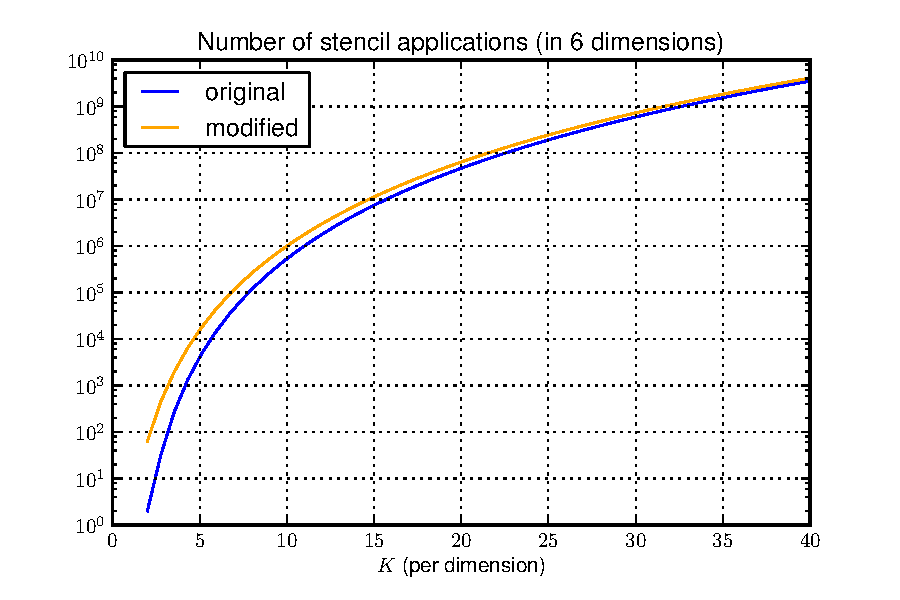
\includegraphics[scale=0.5]{./fig/number_stencil_applications.pdf}
  \caption{Total number of stencil applications for a hypercubic basis shape
           in $D=6$ dimensions and with $K$ nodes along each direction.}
  \label{fig:number_stencil_applications}
\end{figure}


\subsection{Cost of a stencil application}


We define the cost of a stencil application $\mathcal{S} \phi_{\vec{k}}$ as the
number of multiplications which involve a $\phi$. The reason is that we will
evaluate $\phi_{\vec{k}}$ on large grids with many nodes hence $\phi_{\vec{k}}$
is a very long vector.

During the application of the full stencil $\mathcal{S}^D$ we multiply a
$D$ vector by $\phi$ in the first term. In the second one we multiply
a $D \times D$ matrix by a vector of size $D$ containing a (different) $\phi$
in each element. Hence the application $\mathcal{S}^D \phi_k$ has a total cost
of $D^2+D$.

For the modified stencil we only evaluate the first element of the vector equation
and therefore we compute the product of a scalar with $\phi$ and form an inner
product between two vectors of length $D$, one containing a (different) $\phi$
in each element. The application of any modified stencil $\mathcal{S}^D_d$ has
therefore a total cost of $D+1$ which is linear in the number of dimensions.
Figure \ref{fig:cost_stencil_application} shows the cost of both stencils
as a function of dimension $D$.

\begin{figure}
  \centering
  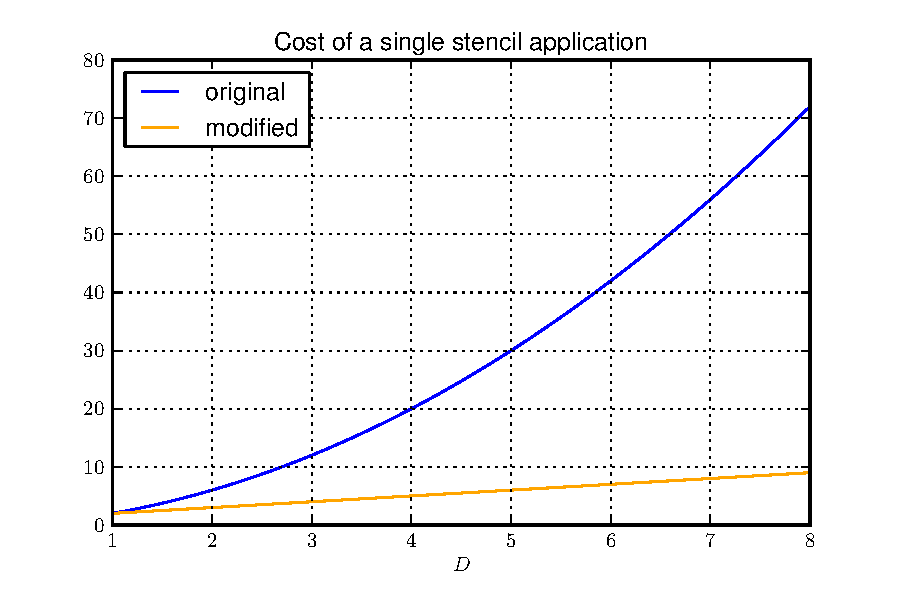
\includegraphics[scale=0.5]{./fig/cost_stencil_application.pdf}
  \caption{The costs of both stencil types in several dimensions.}
  \label{fig:cost_stencil_application}
\end{figure}

If we now compare both evaluation schemes by the number of stencil applications
and the costs of a single application it turns out that the scheme using modified
stencils is much more efficient! In formal notation we find:

\begin{equation*}
  \left(\prod_{d=0}^{D-1} (K_d -1) +1\right) (D^2+D) < \left(\prod_{d=0}^{D-1} K_d -1\right) (D+1)
\end{equation*}

for large enough $K$ where the cross over point depends on the dimension $D$.
For $D = 1$ both schemes are equivalent and have the same costs. Figure
\ref{fig:total_cost_evaluation} shows the overall costs for an hypercubic
basis shape in $D=6$ dimensions.

\begin{figure}
  \centering
  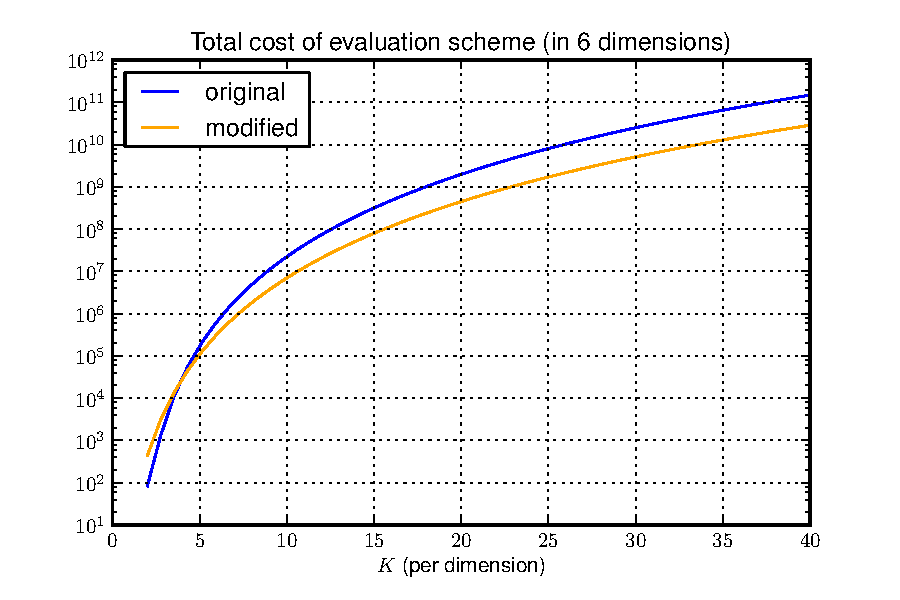
\includegraphics[scale=0.5]{./fig/total_cost_evaluation.pdf}
  \caption{Total cost of a basis evaluation for a hypercubic basis shape
           in $D=6$ dimensions and with $K$ nodes along each direction.}
  \label{fig:total_cost_evaluation}
\end{figure}


\section{Vector-valued wavepackets}


For the purpose of solving the time-dependent Schrödinger equation with non-adiabatic
potentials the scalar wavepackets are not enough. Recall that the potential has $N$
different energy levels. The wavefunction $\Ket{\varphi}$ needs therefore $N$ components
stacked into a vector. In the following we construct \emph{vectorial wavepackets}
where each component is given by a scalar wavepacket. Formally we are in this situation:

\begin{equation}
  \Psi(\vec{x}, t) \assign
  \begin{pmatrix}
    \Phi_0(\vec{x}, t) \\
    \vdots \\
    \Phi_{N-1}(\vec{x}, t)
  \end{pmatrix} \,.
\end{equation}

How many free input parameters does this object have? Each component $\Phi_i$ needs
a set $\Pi_i$ of Hagedorn parameters. (We should write $\Phi_i\left[\Pi_i\right]$
but this becomes lengthy so we drop this soon.) If we use the very same parameter
set $\Pi$ for each component we arrive at what we call a \emph{homogeneous wavepacket}.

\begin{definition}[Homogeneous vectorial wavepacket]
  \begin{equation} \label{eq:vectorial_wavepacket_hom}
    \Ket{\Psi} \assign
    \Psi\left[\Pi\right](\vec{x}, t)
    =
    \begin{pmatrix}
      \Phi_0\left[\Pi\right](\vec{x}, t) \\
      \vdots \\
      \Phi_{N-1}\left[\Pi\right](\vec{x}, t) \\
    \end{pmatrix}
  \end{equation}
  where $\Pi_i \equiv \Pi_j \equiv \Pi \,\forall\, i,j$
\end{definition}

However, at any fixed time each component is independent from all other ones. For
this reason we can choose possibly different sets $\Pi_i$ of parameters for all
$N$ components. By doing this we get an \emph{inhomogeneous wavepacket}, formally
defined as:

\begin{definition}[Inhomogeneous vectorial wavepacket]
  \begin{equation} \label{eq:vectorial_wavepacket_inhom}
    \Ket{\Psi} \assign
    \Psi\left[\Pi_0, \ldots, \Pi_{N-1}\right](\vec{x}, t)
    =
    \begin{pmatrix}
      \Phi_0\left[\Pi_0\right](\vec{x}, t) \\
      \vdots \\
      \Phi_{N-1}\left[\Pi_{N-1}\right](\vec{x}, t) \\
    \end{pmatrix}
  \end{equation}
  where $\Pi_i \neq \Pi_j$ is possible.
\end{definition}

In some applications, for example the spawning approach applied to tunneling
\cite{Gradinaru_semiclassical_tunneling} and the non-adiabatic case
\cite{B_spawning_thesis}, it perfectly makes sense to expand every component
into a different basis of $L^2\left(\mathbb{R}^D\right)$. And since each basis
$\phi_{\vec{k}}$ is essentially fully determined by the parameter set $\Pi$ of
its basis functions $\phi_{\vec{k}}$, this results in different parameter sets
$\Pi_i$ for each component $\Phi_i$.

For some computations we find a more explicit representation of $\Psi$ to be
of greater use. The above definitions can be trivially rewritten as follows by
introducing the unit vectors $\vec{e}^j$ of the canonical basis of $\mathbb{R}^N$.
In the homogeneous case we get:

\begin{equation}
  \Psi\left[\Pi\right](\vec{x}, t) = \sum_{n=0}^{N-1} \vec{e}^n \Phi_n\left[\Pi\right](\vec{x}, t)
\end{equation}

and in the inhomogeneous one:

\begin{equation}
  \Psi\left[\Pi_0,\ldots,\Pi_{N-1}\right](\vec{x}, t) = \sum_{n=0}^{N-1} \vec{e}^n \Phi_n\left[\Pi_n\right](\vec{x}, t) \,.
\end{equation}

We should also note that each component can have an individual basis shape $\mathfrak{K}_n$.
But from now on we will not mention this too often but implicitly assume that each
scalar wavepacket uses the currently best basis shape whatever that means.


\section{Gradient computation}
\label{sec:gradient_computation}


In this section we want to compute the gradient of a scalar wavepacket $\Phi$. More precisely
we find the result of the operator application $-i \varepsilon^2 \nabla \Phi$. From
now on we define the short hand notation $y \assign -i \varepsilon^2 \nabla$. We would
like to have an explicit representation of $y$. Of course it includes just the ordinary
gradient differential operator. But we need a more involved representation allowing us to
easily compute the application of $y$ to a wavepacket of the form given in \eqref{eq:scalar_wavepacket}.
Luckily there is a term of precisely the form of $y$ included in the definition of the
ladder operators in equation \eqref{eq:raising_ops_Dd_explicit}. We proceed by solving the
linear system consisting of the two operator definitions of $\mathcal{L}$ and $\mathcal{R}$
for $y$. We begin by transforming the definition of $\mathcal{R}$ as follows (with the usual
definition of $\theta$):

\begin{align*}
  \mathcal{R} & =  \frac{i}{\sqrt{2\varepsilon^2}} \left( \mat{P}\H (\vec{x}-\vec{q}) - \mat{Q}\H (\vec{y}-\vec{p}) \right) \\
  \mathcal{R} & = \theta \mat{P}\H (\vec{x}-\vec{q}) - \theta \mat{Q}\H (\vec{y}-\vec{p}) \\
  \theta \mat{Q}\H (\vec{y}-\vec{p}) & = -\mathcal{R} + \theta \mat{P}\H (\vec{x}-\vec{q}) \\
  \mat{Q}\H (\vec{y}-\vec{p}) & = -\frac{1}{\theta} \mathcal{R} + \mat{P}\H (\vec{x}-\vec{q}) \,.
\end{align*}

Before we proceed in solving this for $y$ we transform the definition of $\mathcal{L}$
such that we can replace the term $(\vec{x}-\vec{q})$:

\begin{align*}
  \mathcal{L} & = -\theta \mat{P}\T (\vec{x}-\vec{q}) + \theta \mat{Q}\T (\vec{y}-\vec{p}) \\
  \theta \mat{P}\T (\vec{x}-\vec{q}) & = -\mathcal{L} + \theta \mat{Q}\T (\vec{y}-\vec{p}) \\
  \mat{P}\T (\vec{x}-\vec{q}) & = -\frac{1}{\theta}\mathcal{L} + \mat{Q}\T (\vec{y}-\vec{p}) \\
  \vec{x}-\vec{q} & = -\frac{1}{\theta}\mat{P}\Tinv\mathcal{L} + \mat{P}\Tinv\mat{Q}\T (\vec{y}-\vec{p}) \,.
\end{align*}

Then we can plug this into the above equation:

\begin{align*}
  \mat{Q}\H (\vec{y}-\vec{p}) & = -\frac{1}{\theta} \mathcal{R} +
                                  \mat{P}\H \left(-\frac{1}{\theta}\mat{P}\Tinv\mathcal{L} + \mat{P}\Tinv\mat{Q}\T (\vec{y}-\vec{p}) \right) \\
  \mat{Q}\H (\vec{y}-\vec{p}) & = -\frac{1}{\theta} \mathcal{R} +
                                  -\frac{1}{\theta} \mat{P}\H\mat{P}\Tinv\mathcal{L}
                                  +\mat{P}\H\mat{P}\Tinv\mat{Q}\T (\vec{y}-\vec{p}) \\
  \mat{Q}\H \vec{y} - \mat{Q}\H\vec{p} & = -\frac{1}{\theta} \mathcal{R}
                                           -\frac{1}{\theta} \mat{P}\H\mat{P}\Tinv\mathcal{L}
                                           +\mat{P}\H\mat{P}\Tinv\mat{Q}\T \vec{y}
                                           -\mat{P}\H\mat{P}\Tinv\mat{Q}\T\vec{p} \\
  \mat{Q}\H \vec{y} - \mat{P}\H\mat{P}\Tinv\mat{Q}\T \vec{y}
   & = -\frac{1}{\theta} \mathcal{R}
       -\frac{1}{\theta} \mat{P}\H\mat{P}\Tinv\mathcal{L}
       +\mat{Q}\H\vec{p}
       -\mat{P}\H\mat{P}\Tinv\mat{Q}\T\vec{p} \\
  \underbrace{\left(\mat{Q}\H - \mat{P}\H\mat{P}\Tinv\mat{Q}\T\right)}_{**} \vec{y}
   & = -\frac{1}{\theta} \mathcal{R}
       -\frac{1}{\theta} \mat{P}\H\mat{P}\Tinv\mathcal{L}
       +\left(\mat{Q}\H - \mat{P}\H\mat{P}\Tinv\mat{Q}\T\right)\vec{p} \,.
\end{align*}

Our next task is the computation of the subexpression $**$. For this we start again
with the basis relations from \eqref{eq:PQcond_Dd}. For the first one we get:

\begin{align*}
  \mat{Q}\H \mat{P} - \mat{P}\H \mat{Q} & = 2i \id \\
  \mat{Q}\H - \mat{P}\H \mat{Q} \mat{P}\inv & = 2i \mat{P}\inv \\
\end{align*}

and from the second one:

\begin{align*}
  \mat{P}\T \mat{Q} - \mat{Q}\T \mat{P} & = 0 \\
  \mat{Q} - \mat{P}\Tinv \mat{Q}\T \mat{P} & = 0 \\
  \mat{Q} & = \mat{P}\Tinv \mat{Q}\T \mat{P} \,.
\end{align*}

Combining these two results (replacing the second $\mat{Q}$) we obtain:

\begin{align*}
  \mat{Q}\H - \mat{P}\H \mat{P}\Tinv \mat{Q}\T \mat{P} \mat{P}\inv & = 2i \mat{P}\inv \\
  \mat{Q}\H - \mat{P}\H \mat{P}\Tinv \mat{Q}\T & = 2i \mat{P}\inv \,.
\end{align*}

This last line can then be used as a substitution for $**$ above:

\begin{align*}
  2i \mat{P}\inv \vec{y} & = -\frac{1}{\theta} \mathcal{R}
                             -\frac{1}{\theta} \mat{P}\H\mat{P}\Tinv\mathcal{L}
                             +2i \mat{P}\inv \vec{p} \\
  \mat{P}\inv \vec{y} & = -\frac{1}{2i\theta} \mathcal{R}
                          -\frac{1}{2i\theta} \mat{P}\H \mat{P}\Tinv \mathcal{L}
                          +\mat{P}\inv \vec{p} \\
  \vec{y} & = -\frac{1}{2i\theta} \mat{P}\mathcal{R}
                          -\frac{1}{2i\theta} \mat{P} \mat{P}\H \mat{P}\Tinv \mathcal{L}
                          +\vec{p} \,.
\end{align*}

Finally cleaning up and undoing the introduction of $\theta$ we arrive at:

\begin{equation}
  \vec{y} = \sqrt{\frac{\varepsilon^2}{2}} \left( \mat{P}\mathcal{R} + \mat{\conj{P}} \mathcal{L} \right) + \vec{p} \,.
\end{equation}

If we had begun by using the operators $\mathcal{L}$ and $\mathcal{R}$ in the opposite order
we would have got the complex conjugate equation:

\begin{equation}
  \vec{y} = \sqrt{\frac{\varepsilon^2}{2}} \left( \conj{\mat{P}}\mathcal{L} + \mat{P} \mathcal{R} \right) + \vec{p} \,.
\end{equation}

We can simplify the matrix product $\mat{P} \mat{P}\H \mat{P}\Tinv$ to obtain $\mat{\conj{P}}$.
The reason is the conditions \eqref{eq:PQcond_Dd} which must be fulfilled by
$\mat{P}$ and $\mat{Q}$, see \cite{H_ladder_operators}.


\subsection{Applying the gradient operator}


With this explicit representation of the $y$ operator in terms of raising
and lowering operators we can now study its application to an arbitrary
basis function $\phi_{\vec{k}}$. In the end we then need to apply $y$ to the
whole scalar wavepacket $\Phi$ in order to find its kinetic energy.

What do we have to expect when applying $y$ to a basis function $\phi_{\vec{k}}$?
First, we know that the gradient is defined as usual as:

\begin{equation*}
  \nabla_{\vec{x}} \assign
  \begin{pmatrix}
    \pdiff{}{x_0} \\
    \vdots \\
    \pdiff{}{x_{D-1}} \\
  \end{pmatrix} \,.
\end{equation*}

Hence we have to expect that the gradient applied to $\phi_{\vec{k}}:\mathbb{R}^D\rightarrow\mathbb{C}$
is a vector with $D$ components. Next we conclude from \eqref{eq:raising_ops_Dd_vectorial} that the
ladder operators applied to a function give another vector of same shape. We wish to compute:

\begin{equation*}
  y \phi_{\vec{k}}(\vec{x}) = \sqrt{\frac{\varepsilon^2}{2}} \left( \mat{P}\mathcal{R} + \conj{\mat{P}} \mathcal{L} \right) \phi_{\vec{k}}(\vec{x})
                              + \vec{p} \phi_{\vec{k}}(\vec{x})
\end{equation*}

and if we carry out the application of the ladder operators we get step by step
the following relation for the gradient of a single basis function:

\begin{equation*}
  y \phi_{\vec{k}}(\vec{x}) =
  \sqrt{\frac{\varepsilon^2}{2}} \left(
  \mat{P}
    \begin{pmatrix}
      \mathcal{R}_0 \\
      \vdots \\
      \mathcal{R}_{D-1}
    \end{pmatrix}
  + \conj{\mat{P}}
    \begin{pmatrix}
      \mathcal{L}_0 \\
      \vdots \\
      \mathcal{L}_{D-1}
    \end{pmatrix}
  \right) \phi_{\vec{k}}(\vec{x})
  + \vec{p} \phi_{\vec{k}}(\vec{x})
\end{equation*}

where we apply the ladder operators now:

\begin{equation} \label{eq:grad_basis_function_DD}
  y \phi_{\vec{k}}(\vec{x})
  =
  \sqrt{\frac{\varepsilon^2}{2}}
  \left(
    \mat{P}
    \begin{pmatrix}
      \sqrt{k_0 + 1} \phi_{\vec{k}+\vec{e}^0} \\
      \vdots \\
      \sqrt{k_{D-1} + 1} \phi_{\vec{k}+\vec{e}^{D-1}}
    \end{pmatrix}
    +
    \conj{\mat{P}}
    \begin{pmatrix}
      \sqrt{k_0} \phi_{\vec{k}-\vec{e}^0} \\
      \vdots \\
      \sqrt{k_{D-1}} \phi_{\vec{k}-\vec{e}^{D-1}}
    \end{pmatrix}
  \right)
  + \vec{p} \phi_{\vec{k}} \,.
\end{equation}

This is just for one single basis function. But we need more.
Thus we compute the gradient of a whole scalar wavepacket
$\Phi = \sum_{\vec{k}\in\mathfrak{K}} c_{\vec{k}}\phi_{\vec{k}}$:

\begin{equation*}
  y \Phi
  = \sum_{\vec{k}\in\mathfrak{K}} y \, c_{\vec{k}}\phi_{\vec{k}}
  = \sum_{\vec{k}\in\mathfrak{K}} c_{\vec{k}} \, y \phi_{\vec{k}}
\end{equation*}

For a shorter notation we define the following variables:

\begin{align*}
  \theta & \assign \sqrt{\frac{\varepsilon^2}{2}} \\
  \vec{\alpha}(\phi_{\vec{k}}) & \assign
     \begin{pmatrix}
      \sqrt{k_0 + 1} \phi_{\vec{k}+\vec{e}^0} \\
      \vdots \\
      \sqrt{k_{D-1} + 1} \phi_{\vec{k}+\vec{e}^{D-1}}
    \end{pmatrix} \\
  \vec{\beta}(\phi_{\vec{k}}) & \assign
    \begin{pmatrix}
      \sqrt{k_0} \phi_{\vec{k}-\vec{e}^0} \\
      \vdots \\
      \sqrt{k_{D-1}} \phi_{\vec{k}-\vec{e}^{D-1}}
    \end{pmatrix} \,.
\end{align*}

Continuing we derive:

\begin{align*}
  & = \sum_{\vec{k}\in\mathfrak{K}}
        \left(
          c_{\vec{k}} \vec{p} \phi_{\vec{k}}
          + \theta c_{\vec{k}} \mat{P} \vec{\alpha}(\phi_{\vec{k}})
          + \theta c_{\vec{k}} \conj{\mat{P}} \vec{\beta}(\phi_{\vec{k}})
        \right) \nonumber\\
  & = \sum_{\vec{k}\in\mathfrak{K}} c_{\vec{k}} \vec{p} \phi_{\vec{k}}
    + \sum_{\vec{k}\in\mathfrak{K}} \theta c_{\vec{k}} \mat{P} \vec{\alpha}(\phi_{\vec{k}})
    + \sum_{\vec{k}\in\mathfrak{K}} \theta c_{\vec{k}} \conj{\mat{P}} \vec{\beta}(\phi_{\vec{k}}) \,.
\end{align*}

It becomes obvious that $y \phi_{\vec{k}}$ has contributions from all neighbours
$\phi_{\vec{k} + \vec{e}^d}$ and $\phi_{\vec{k} - \vec{e}^d}$ for all $d \in [0, \ldots, D-1]$
and from $\phi_{\vec{k}}$. This immediately raises the question of an efficient
computation. In the end we will need $y \phi_{\vec{k}}$ for all $\vec{k} \in \mathfrak{K}$.
Since there are ladder operators involved we have to be careful for all $\vec{k}$
on the border of $\mathfrak{K}$ who don't have a full set of neighbours in all
directions $d$. For each neighbour $\vec{k}\pm\vec{e}^d$ that is not part of the
basis shape $\mathfrak{K}$ we have to decide what to do. And the rules are as follows.

If the vector $\vec{k}-\vec{e}^d$ has negative components, then we can take the
corresponding basis function to be equivalent zero. We call this situation an
\emph{underflow} \footnote{ This has nothing to do with the usual arithmetic
over/underflow. It just serves as a notation of \emph{where} we access elements
outside of our basis shape $\mathfrak{K}$.}.

The other case is more involved. The functions $\phi_{\vec{k}}$ clearly never
vanish identically zero. However we only have finite linear combinations $\Phi$ of
basis functions $\phi_{\vec{k}}$. Hence all coefficients for sufficiently \emph{large}
$\vec{k}$ vanish. And finally we are only interested in the new coefficients
$c_{\vec{k}}^{\prime i}$ of each component $i$ of the gradient $y \phi_{\vec{k}}$. For
this reason we can also insert zeros in the case such an \emph{overflow} occurs.
For an example of the situation and the issues that may arise refer to figure
\ref{fig:grad_phi_kl_stencil}.

\begin{figure}
  \centering
  \begin{tikzpicture}[%
    func/.style={scale=0.8,color=gray},
    zero/.style={scale=0.8,color=gray}]

    \node[zero, color=black] (v0m1) at (1,0) {$0$};
    \node[zero] (v1m1) at (2,0) {$0$};
    \node[zero] (v2m1) at (3,0) {$0$};
    \node[zero] (v3m1) at (4,0) {$0$};
    \node[zero] (v4m1) at (5,0) {$0$};
    \node[zero] (v5m1) at (6,0) {$0$};
    %\node[zero] (v6m1) at (7,0) {$0$};

    \node[zero, color=black] (vm10) at (0,1) {$0$};
    \node[zero] (vm11) at (0,2) {$0$};
    \node[zero] (vm12) at (0,3) {$0$};
    \node[zero] (vm13) at (0,4) {$0$};
    \node[zero, color=black] (vm14) at (0,5) {$0$};
    %\node[zero] (vm15) at (0,6) {$0$};

    \node[func, color=black] (v00) at (1,1) {$\phi_{0,0}$};
    \node[func, color=black] (v01) at (1,2) {$\phi_{0,1}$};
    \node[func] (v02) at (1,3) {$\phi_{0,2}$};
    \node[func, color=black] (v03) at (1,4) {$\phi_{0,3}$};
    \node[func, color=black] (v04) at (1,5) {$\phi_{0,4}$};
    \node[func, color=black] (v05) at (1,6) {$\phi_{0,5}$};

    \node[func, color=black] (v10) at (2,1) {$\phi_{1,0}$};
    \node[func] (v11) at (2,2) {$\phi_{1,1}$};
    \node[func] (v12) at (2,3) {$\phi_{1,2}$};
    \node[func] (v13) at (2,4) {$\phi_{1,3}$};
    \node[func, color=black] (v14) at (2,5) {$\phi_{1,4}$};
    \node[func] (v15) at (2,6) {$\phi_{1,5}$};

    \node[func] (v20) at (3,1) {$\phi_{2,0}$};
    \node[func] (v21) at (3,2) {$\phi_{2,1}$};
    \node[func, color=black] (v22) at (3,3) {$\phi_{2,2}$};
    \node[func] (v23) at (3,4) {$\phi_{2,3}$};
    \node[func] (v24) at (3,5) {$\phi_{2,4}$};
    \node[func] (v25) at (3,6) {$\phi_{2,5}$};

    \node[func] (v30) at (4,1) {$\phi_{3,0}$};
    \node[func, color=black] (v31) at (4,2) {$\phi_{3,1}$};
    \node[func, color=black] (v32) at (4,3) {$\phi_{3,2}$};
    \node[func, color=black] (v33) at (4,4) {$\phi_{3,3}$};
    \node[func] (v34) at (4,5) {$\phi_{3,4}$};
    \node[func] (v35) at (4,6) {$\phi_{3,5}$};

    \node[func] (v40) at (5,1) {$\phi_{4,0}$};
    \node[func] (v41) at (5,2) {$\phi_{4,1}$};
    \node[func, color=black] (v42) at (5,3) {$\phi_{4,2}$};
    \node[func] (v43) at (5,4) {$\phi_{4,3}$};
    \node[func, color=black] (v44) at (5,5) {$\phi_{4,4}$};
    \node[func] (v45) at (5,6) {$\phi_{4,5}$};

    \node[func] (v50) at (6,1) {$\phi_{5,0}$};
    \node[func] (v51) at (6,2) {$\phi_{5,1}$};
    \node[func] (v52) at (6,3) {$\phi_{5,2}$};
    \node[func, color=black] (v53) at (6,4) {$\phi_{5,3}$};
    \node[func, color=black] (v54) at (6,5) {$\phi_{5,4}$};
    \node[func, color=black] (v55) at (6,6) {$\phi_{5,5}$};

    \node[func] (v60) at (7,1) {$\phi_{6,0}$};
    \node[func] (v61) at (7,2) {$\phi_{6,1}$};
    \node[func] (v62) at (7,3) {$\phi_{6,2}$};
    \node[func] (v63) at (7,4) {$\phi_{6,3}$};
    \node[func, color=black] (v64) at (7,5) {$\phi_{6,4}$};
    %\node[func] (v65) at (7,6) {$\phi_{6,5}$};

    \begin{scope}
    \draw[draw=black,line width=0.7pt] ($(v00)+(0.0,-0.5)$)
        to[out=0,in=180] ($(v50)+(0.0,-0.5)$)
        to[out=0,in=270] ($(v50)+(0.5,0.0)$)
        to[out=90,in=270] ($(v54)+(0.5,0.0)$)
        to[out=90,in=0] ($(v54)+(0.0,0.5)$)
        to[out=180,in=0] ($(v04)+(0.0,0.5)$)
        to[out=180,in=90] ($(v04)+(-0.5,0.0)$)
        to[out=270,in=90] ($(v00)+(-0.5,0.0)$)
        to[out=270,in=180] ($(v00)+(0.0,-0.5)$);
    \end{scope}

    % lower left
    \begin{scope}
    \draw[draw=blue!100,line width=0.8pt] ($(vm10)+(0.0,0.3)$)
        to[out=170,in=90] ($(vm10)+(-0.3,0.0)$)
        to[out=270,in=190] ($(vm10)+(0.0,-0.3)$)
        to[out=10,in=80] ($(v0m1)+(-0.3,0.0)$)
        to[out=260,in=180] ($(v0m1)+(0.0,-0.3)$)
        to[out=0,in=280] ($(v0m1)+(0.3,0.0)$)
        to[out=100,in=350] ($(vm10)+(0.0,0.3)$);
    \end{scope}
    \begin{scope}
    \draw[draw=orange!100,line width=0.8pt] ($(v10)-(0.0,0.3)$)
        to[out=10,in=170] ($(v10)-(0.0,0.3)$)
        to[out=0,in=270] ($(v10)-(-0.3,0.0)$)
        to[out=90,in=10] ($(v10)-(0.0,-0.3)$)
        to[out=190,in=260] ($(v01)-(-0.3,0.0)$)
        to[out=80,in=0] ($(v01)-(0.0,-0.3)$)
        to[out=180,in=100] ($(v01)-(0.3,0.0)$)
        to[out=280,in=170] ($(v10)-(0.0,0.3)$);
    \end{scope}
    \begin{scope}
    \draw[draw=gray!100,line width=0.8pt] ($(v00)-(0.0,0.3)$)
        to[out=180,in=270] ($(v00)-(0.3,0.0)$)
        to[out=90,in=180] ($(v00)+(0.0,0.3)$)
        to[out=0,in=90] ($(v00)+(0.3,0.0)$)
        to[out=270,in=0] ($(v00)-(0.0,0.3)$);
    \end{scope}

    % upper left
    \begin{scope}
    \draw[draw=blue!100,line width=0.8pt] ($(vm14)+(0.0,0.3)$)
        to[out=170,in=90] ($(vm14)+(-0.3,0.0)$)
        to[out=270,in=190] ($(vm14)+(0.0,-0.3)$)
        to[out=10,in=80] ($(v03)+(-0.3,0.0)$)
        to[out=260,in=180] ($(v03)+(0.0,-0.3)$)
        to[out=0,in=280] ($(v03)+(0.3,0.0)$)
        to[out=100,in=350] ($(vm14)+(0.0,0.3)$);
    \end{scope}
    \begin{scope}
    \draw[draw=orange!100,line width=0.8pt] ($(v14)-(0.0,0.3)$)
        to[out=10,in=170] ($(v14)-(0.0,0.3)$)
        to[out=0,in=270] ($(v14)-(-0.3,0.0)$)
        to[out=90,in=10] ($(v14)-(0.0,-0.3)$)
        to[out=190,in=260] ($(v05)-(-0.3,0.0)$)
        to[out=80,in=0] ($(v05)-(0.0,-0.3)$)
        to[out=180,in=100] ($(v05)-(0.3,0.0)$)
        to[out=280,in=170] ($(v14)-(0.0,0.3)$);
    \end{scope}
    \begin{scope}
    \draw[draw=gray!100,line width=0.8pt] ($(v04)-(0.0,0.3)$)
        to[out=180,in=270] ($(v04)-(0.3,0.0)$)
        to[out=90,in=180] ($(v04)+(0.0,0.3)$)
        to[out=0,in=90] ($(v04)+(0.3,0.0)$)
        to[out=270,in=0] ($(v04)-(0.0,0.3)$);
    \end{scope}

    % upper right
    \begin{scope}
    \draw[draw=blue!100,line width=0.8pt] ($(v44)+(0.0,0.3)$)
        to[out=170,in=90] ($(v44)+(-0.3,0.0)$)
        to[out=270,in=190] ($(v44)+(0.0,-0.3)$)
        to[out=10,in=80] ($(v53)+(-0.3,0.0)$)
        to[out=260,in=180] ($(v53)+(0.0,-0.3)$)
        to[out=0,in=280] ($(v53)+(0.3,0.0)$)
        to[out=100,in=350] ($(v44)+(0.0,0.3)$);
    \end{scope}
    \begin{scope}
    \draw[draw=orange!100,line width=0.8pt] ($(v64)-(0.0,0.3)$)
        to[out=10,in=170] ($(v64)-(0.0,0.3)$)
        to[out=0,in=270] ($(v64)-(-0.3,0.0)$)
        to[out=90,in=10] ($(v64)-(0.0,-0.3)$)
        to[out=190,in=260] ($(v55)-(-0.3,0.0)$)
        to[out=80,in=0] ($(v55)-(0.0,-0.3)$)
        to[out=180,in=100] ($(v55)-(0.3,0.0)$)
        to[out=280,in=170] ($(v64)-(0.0,0.3)$);
    \end{scope}
    \begin{scope}
    \draw[draw=gray!100,line width=0.8pt] ($(v54)-(0.0,0.3)$)
        to[out=180,in=270] ($(v54)-(0.3,0.0)$)
        to[out=90,in=180] ($(v54)+(0.0,0.3)$)
        to[out=0,in=90] ($(v54)+(0.3,0.0)$)
        to[out=270,in=0] ($(v54)-(0.0,0.3)$);
    \end{scope}

    % central
    \begin{scope}
    \draw[draw=blue!100,line width=0.8pt] ($(v22)+(0.0,0.3)$)
        to[out=170,in=90] ($(v22)+(-0.3,0.0)$)
        to[out=270,in=190] ($(v22)+(0.0,-0.3)$)
        to[out=10,in=80] ($(v31)+(-0.3,0.0)$)
        to[out=260,in=180] ($(v31)+(0.0,-0.3)$)
        to[out=0,in=280] ($(v31)+(0.3,0.0)$)
        to[out=100,in=350] ($(v22)+(0.0,0.3)$);
    \end{scope}
    \begin{scope}
    \draw[draw=orange!100,line width=0.8pt] ($(v42)-(0.0,0.3)$)
        to[out=10,in=170] ($(v42)-(0.0,0.3)$)
        to[out=0,in=270] ($(v42)-(-0.3,0.0)$)
        to[out=90,in=10] ($(v42)-(0.0,-0.3)$)
        to[out=190,in=260] ($(v33)-(-0.3,0.0)$)
        to[out=80,in=0] ($(v33)-(0.0,-0.3)$)
        to[out=180,in=100] ($(v33)-(0.3,0.0)$)
        to[out=280,in=170] ($(v42)-(0.0,0.3)$);
    \end{scope}
    \begin{scope}
    \draw[draw=gray!100,line width=0.8pt] ($(v32)-(0.0,0.3)$)
        to[out=180,in=270] ($(v32)-(0.3,0.0)$)
        to[out=90,in=180] ($(v32)+(0.0,0.3)$)
        to[out=0,in=90] ($(v32)+(0.3,0.0)$)
        to[out=270,in=0] ($(v32)-(0.0,0.3)$);
    \end{scope}
\end{tikzpicture}

  \caption[Computing the gradient in two dimensions] {Stencil application for
           computing the gradient $y \phi_{\vec{k}}$ for different $\vec{k}$ in
           two dimensions. For each computation we need the function itself
           (grey circles), the backward neighbours $\phi_{\vec{k}-\vec{e}^d}$
           (blue contours) and the forward neighbours $\phi_{\vec{k}+\vec{e}^d}$
           (orange contours). Clearly we need additional functions outside of
           the basis shape $\mathfrak{K}$ (black rectangle). In all corners
            and along all sides we under- and overflow respectively.}
  \label{fig:grad_phi_kl_stencil}
\end{figure}

Before we continue let's make a not so small but very simple example. Assume
the hypercubic basis shape in two dimensions is $\mathfrak{K} = \vec{K} = (3,3)$.
The wavepacket consists of the following linear combination:

\begin{align*}
  \Phi \assign \, & c_{0,0} \phi_{0,0} + c_{1,0} \phi_{1,0} + c_{2,0} \phi_{2,0} \\
             + \, & c_{0,1} \phi_{0,1} + c_{1,1} \phi_{1,1} + c_{2,1} \phi_{2,1} \\
             + \, & c_{0,2} \phi_{0,2} + c_{1,2} \phi_{1,2} + c_{2,2} \phi_{2,2} \,.
\end{align*}

Computing the gradients individually for some of the terms we get:

\begin{center}
\begin{tabular}{ll}
Multi-index node  & Gradient \\
\hline \\
$\vec{k} = (0,0)$ & $c_{0,0} \, \vec{p} \phi_{0,0} +
                     \theta c_{0,0} \, \mat{P} \begin{pmatrix} \sqrt{1} \, \phi_{1,0} \\
                                                               \sqrt{1} \, \phi_{0,1}
                                               \end{pmatrix} +
                     \theta c_{0,0} \, \conj{\mat{P}} \begin{pmatrix} \sqrt{0} \, \phi_{-1,0} \\
                                                                      \sqrt{0} \, \phi_{0,-1}
                                                      \end{pmatrix}$\\
$\vec{k} = (1,0)$ & $c_{1,0} \, \vec{p} \phi_{1,0} +
                     \theta c_{1,0} \, \mat{P} \begin{pmatrix} \sqrt{2} \, \phi_{2,0} \\
                                                               \sqrt{1} \, \phi_{1,1}
                                               \end{pmatrix} +
                     \theta c_{1,0} \, \conj{\mat{P}} \begin{pmatrix} \sqrt{1} \, \phi_{0,0} \\
                                                                      \sqrt{0} \, \phi_{1,-1}
                                                      \end{pmatrix}$\\
$\vec{k} = (0,1)$ & $c_{0,1} \, \vec{p} \phi_{0,1} +
                     \theta c_{0,1} \, \mat{P} \begin{pmatrix} \sqrt{1} \, \phi_{1,1} \\
                                                               \sqrt{2} \, \phi_{0,2}
                                               \end{pmatrix} +
                     \theta c_{0,1} \, \conj{\mat{P}} \begin{pmatrix} \sqrt{0} \, \phi_{-1,1} \\
                                                                      \sqrt{1} \, \phi_{0,0}
                                                      \end{pmatrix}$\\
$\vec{k} = (1,1)$ & $c_{1,1} \, \vec{p} \phi_{1,1} +
                     \theta c_{1,1} \, \mat{P} \begin{pmatrix} \sqrt{2} \, \phi_{2,1} \\
                                                               \sqrt{2} \, \phi_{1,2}
                                               \end{pmatrix} +
                     \theta c_{1,1} \, \conj{\mat{P}} \begin{pmatrix} \sqrt{1} \, \phi_{0,1} \\
                                                                      \sqrt{1} \, \phi_{1,0}
                                                      \end{pmatrix}$ \\
$\vec{k} = (2,1)$ & $c_{2,1} \, \vec{p} \phi_{2,1} +
                     \theta c_{2,1} \, \mat{P} \begin{pmatrix} \sqrt{3} \, \phi_{3,1} \\
                                                               \sqrt{2} \, \phi_{2,2}
                                               \end{pmatrix} +
                     \theta c_{2,1} \, \conj{\mat{P}} \begin{pmatrix} \sqrt{2} \, \phi_{1,1} \\
                                                                      \sqrt{1} \, \phi_{2,0}
                                                      \end{pmatrix}$ \\
$\vec{k} = (1,2)$ & $c_{1,2} \, \vec{p} \phi_{1,2} +
                     \theta c_{1,2} \, \mat{P} \begin{pmatrix} \sqrt{2} \, \phi_{2,2} \\
                                                               \sqrt{3} \, \phi_{1,3}
                                               \end{pmatrix} +
                     \theta c_{1,2} \, \conj{\mat{P}} \begin{pmatrix} \sqrt{1} \, \phi_{0,2} \\
                                                                      \sqrt{2} \, \phi_{1,1}
                                                      \end{pmatrix}$ \\
$\vdots$ & $\hdots$
\end{tabular}
\end{center}

and we would sum up all these terms to get the overall gradient of $\Phi$. In this form however
it is not of much use to us. We want to represent the gradient again as linear combinations
over the same set of basis functions:

\begin{equation} \label{eq:gradient_basis_expandion}
  y \Phi = \sum_{\vec{k} \in \overline{\mathfrak{K}}} \vec{c}^\prime_{\vec{k}} \phi_{\vec{k}}
\end{equation}

where $\vec{c}^\prime_{\vec{k}} \in \mathbb{C}^{D}$ and $\overline{\mathfrak{K}}$ is the
extended basis shape (in case of our example $\overline{\mathfrak{K}} = \vec{K}^\prime = (4,4)$).
This is indeed possible, expanding the fourth row from the table above in
instances of $\phi_{\vec{k}}$ and summing up we get:

\begin{equation*}
    c_{1,1} \, \vec{p} \phi_{1,1}
  + \theta c_{1,1} \, \sqrt{2} \, \mat{P}_{:,0} \phi_{2,1}
  + \theta c_{1,1} \, \sqrt{2} \, \mat{P}_{:,1} \phi_{1,2}
  + \theta c_{1,1} \, \conj{\mat{P}}_{:,0} \phi_{0,1}
  + \theta c_{1,1} \, \conj{\mat{P}}_{:,1} \phi_{1,0} \,.
\end{equation*}

In finding the coefficient $\vec{c}_{1,1}$ of $\phi_{1,1}$ we have to be very careful, because
there are further terms on up to 4 other rows that contribute to $\vec{c}_{1,1}$.
(Note that this coefficient is a good example as its lattice node has a full set
of 4 neighbours.) Summing up all relevant terms we find that:

\begin{equation*}
  \vec{c}^\prime_{1,1} = c_{1,1} \, \vec{p}
+ \theta c_{0,1} \, \mat{P}_{:,0} \,.
+ \theta c_{1,0} \, \mat{P}_{:,1}
+ \theta c_{2,1} \, \sqrt{2} \, \conj{\mat{P}}_{:,0}
+ \theta c_{1,2} \, \sqrt{2} \, \conj{\mat{P}}_{:,1} \,.
\end{equation*}

The last four terms can be recombined into one per pair and we end up with:

\begin{equation*}
  \vec{c}^\prime_{1,1} = c_{1,1} \, \vec{p}
+ \theta \mat{P}
  \begin{pmatrix}
    c_{0,1} \\ c_{1,0}
  \end{pmatrix}
+ \theta \conj{\mat{P}}
  \begin{pmatrix}
    \sqrt{2} \, c_{2,1} \\ \sqrt{2} \, c_{1,2}
  \end{pmatrix}
\end{equation*}

Doing these transformations in a systematic way is the major issue in computing the gradients.
With a bit of guessing we can find the following general rule for the coefficient vectors
$\vec{c}^\prime_{\vec{k}}$ for all $\vec{k} \in \overline{\mathfrak{K}}$:

\begin{equation*}
  \vec{c}^\prime_{\vec{k}} = c_{\vec{k}} \, \vec{p}
                             + \sqrt{\frac{\varepsilon^2}{2}} \sum_{d=0}^{D-1} c_{\vec{k}+\vec{e}^d} \, \sqrt{\vec{k}_{d}+1} \, \conj{\mat{P}}_{:,d}
                             + \sqrt{\frac{\varepsilon^2}{2}} \sum_{d=0}^{D-1} c_{\vec{k}-\vec{e}^d} \, \sqrt{\vec{k}_{d}} \, \mat{P}_{:,d}
\end{equation*}

which again can be cast in compact form:

\begin{equation} \label{eq:gradient_coefficients_DD}
  \vec{c}^\prime_{\vec{k}} = c_{\vec{k}} \, \vec{p}
                             + \sqrt{\frac{\varepsilon^2}{2}} \left(
                               \conj{\mat{P}}
                               \begin{pmatrix}
                                 c_{\vec{k}+\vec{e}^0} \, \sqrt{\vec{k}_{0}+1} \\
                                 \vdots \\
                                 c_{\vec{k}+\vec{e}^{D-1}} \, \sqrt{\vec{k}_{D-1}+1}
                               \end{pmatrix}
                             + \mat{P}
                               \begin{pmatrix}
                                 c_{\vec{k}-\vec{e}^0} \, \sqrt{\vec{k}_{0}} \\
                                 \vdots \\
                                 c_{\vec{k}-\vec{e}^{D-1}} \, \sqrt{\vec{k}_{D-1}}
                               \end{pmatrix}
                               \right) \,.
\end{equation}


\subsection{Gather-type algorithm}


The most simple algorithm to compute $y \phi_{\vec{k}}$ for all $\vec{k} \in \mathfrak{K}$
has to iterate over all $\vec{k} \in \overline{\mathfrak{K}}$ and apply the
two stencils to get the data from backward and forward neighbours of $\vec{k}$
and to compute $y \phi_{\vec{k}}$ by the formula \eqref{eq:gradient_coefficients_DD}.
This is simple to understand and works reasonably efficient. We call this algorithm the
\emph{gather-type} stencil application.

The only not so easy point here is that we can not iterate just over $\mathfrak{K}$
but have to extend the basis shape due to the nature of the neighbourhood stencil.
In more detail, this is necessary as there are $\vec{k}^\prime \notin \mathfrak{K}$
for which the above formula \eqref{eq:gradient_coefficients_DD} still yields a non-zero result since
the stencil centred at $\vec{k}^\prime$ still overlaps with the basis shape $\mathfrak{K}$.
And we do not want to loose these contributions. Therefore we extend the basis shape
$\mathfrak{K}$ by one node in all directions and get what we denote by $\overline{\mathfrak{K}}$.
This should be clear by looking at figure \ref{fig:grad_phi_kl_stencil}.

In one single space dimension $x$ the gradient equals the derivative and the result
is not a vector of functions but just a function too. Therefore it is easier to
understand the gradient computation for one-dimensional wavepackets $\Phi(x)$ first.
The whole process of the gather-type algorithm is shown in figure
\ref{fig:grad_phi_kl_gather_stencil_1D} in considerable detail.

\begin{figure}
  \centering
  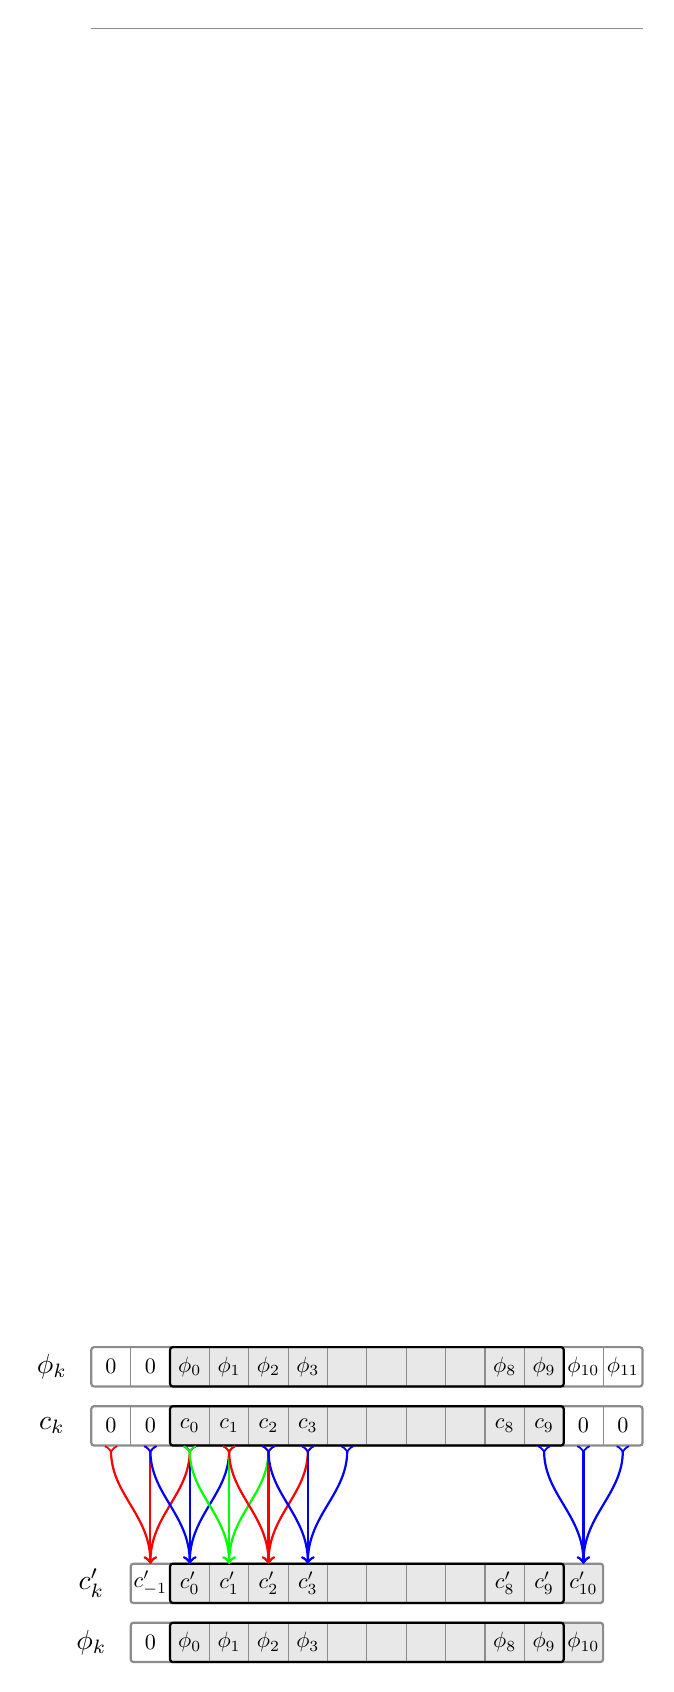
\begin{tikzpicture}
  \coordinate (com2) at (-0.75, 2.0);
  \coordinate (com1) at (-0.25, 2.0);
  \coordinate (co0) at (0.25, 2.0);
  \coordinate (co1) at (0.75, 2.0);
  \coordinate (co2) at (1.25, 2.0);
  \coordinate (co3) at (1.75, 2.0);
  \coordinate (co4) at (2.25, 2.0);
  \coordinate (co5) at (2.75, 2.0);
  \coordinate (co6) at (3.25, 2.0);
  \coordinate (co9) at (4.75, 2.0);
  \coordinate (co10) at (5.25, 2.0);
  \coordinate (co11) at (5.75, 2.0);

  \coordinate (cpm1) at (-0.25, 0.5);
  \coordinate (cp0) at (0.25, 0.5);
  \coordinate (cp1) at (0.75, 0.5);
  \coordinate (cp2) at (1.25, 0.5);
  \coordinate (cp3) at (1.75, 0.5);
  \coordinate (cp4) at (2.25, 0.5);
  \coordinate (cp5) at (2.75, 0.5);
  \coordinate (cp6) at (3.25, 0.5);
  \coordinate (cp8) at (4.25, 0.5);
  \coordinate (cp9) at (4.75, 0.5);
  \coordinate (cp10) at (5.25, 0.5);

  % upper
  \fill[gray!20, rounded corners=1] (0.0,2.75) rectangle (5.0,3.25);
  \draw[step=5mm, ystep=20cm, gray] (-1.0,2.75) grid (6.0,3.25);
  \draw[gray, thick, rounded corners=1] (-1.0,2.75) rectangle (6.0,3.25);
  \draw[black, thick, rounded corners=1] (0.0,2.75) rectangle (5.0,3.25);

  \fill[gray!20, rounded corners=1] (0.0,2.0) rectangle (5.0,2.5);
  \draw[step=5mm, gray] (-1.0,2.0) grid (6.0,2.5);
  \draw[gray, thick, rounded corners=1] (-1.0,2.0) rectangle (6.0,2.5);
  \draw[black, thick, rounded corners=1] (0.0,2.0) rectangle (5.0,2.5);

  % lower
  \fill[gray!20, rounded corners=1] (0.0,-0.75) rectangle (5.5,-0.25);
  \draw[step=5mm, ystep=20cm, gray] (0.0,-0.75) grid (5.0,-0.25);
  \draw[gray, thick, rounded corners=1] (-0.5,-0.75) rectangle (5.5,-0.25);
  \draw[black, thick, rounded corners=1] (0.0,-0.75) rectangle (5.0,-0.25);

  \fill[gray!20, rounded corners=1] (0.0,0.0) rectangle (5.5,0.5);
  \draw[step=5mm, gray] (0.0,0.0) grid (5.0,0.5);
  \draw[gray, thick, rounded corners=1] (-0.5,0.0) rectangle (5.5,0.5);
  \draw[black, thick, rounded corners=1] (0.0,0.0) rectangle (5.0,0.5);

  \draw[>->, thick, color=red] (com2) to[out=270,in=90] (cpm1);
  \draw[>->, thick, color=red] (com1) to[out=270,in=90] (cpm1);
  \draw[>->, thick, color=red] (co0) to[out=270,in=90] (cpm1);

  \draw[>->, thick, color=blue] (com1) to[out=270,in=90] (cp0);
  \draw[>->, thick, color=blue] (co0) to[out=270,in=90] (cp0);
  \draw[>->, thick, color=blue] (co1) to[out=270,in=90] (cp0);

  \draw[>->, thick, color=green] (co0) to[out=270,in=90] (cp1);
  \draw[>->, thick, color=green] (co1) to[out=270,in=90] (cp1);
  \draw[>->, thick, color=green] (co2) to[out=270,in=90] (cp1);

  \draw[>->, thick, color=red] (co1) to[out=270,in=90] (cp2);
  \draw[>->, thick, color=red] (co2) to[out=270,in=90] (cp2);
  \draw[>->, thick, color=red] (co3) to[out=270,in=90] (cp2);

  \draw[>->, thick, color=blue] (co2) to[out=270,in=90] (cp3);
  \draw[>->, thick, color=blue] (co3) to[out=270,in=90] (cp3);
  \draw[>->, thick, color=blue] (co4) to[out=270,in=90] (cp3);

  \draw[>->, thick, color=blue] (co9) to[out=270,in=90] (cp10);
  \draw[>->, thick, color=blue] (co10) to[out=270,in=90] (cp10);
  \draw[>->, thick, color=blue] (co11) to[out=270,in=90] (cp10);

  \node[scale=0.8] at (-0.75,2.25) [black] {$0$};
  \node[scale=0.8] at (-0.25,2.25) [black] {$0$};
  \node[scale=0.8] at (0.25,2.25) [black] {$c_0$};
  \node[scale=0.8] at (0.75,2.25) [black] {$c_1$};
  \node[scale=0.8] at (1.25,2.25) [black] {$c_2$};
  \node[scale=0.8] at (1.75,2.25) [black] {$c_3$};
  \node[scale=0.8] at (4.25,2.25) [black] {$c_8$};
  \node[scale=0.8] at (4.75,2.25) [black] {$c_9$};
  \node[scale=0.8] at (5.25,2.25) [black] {$0$};
  \node[scale=0.8] at (5.75,2.25) [black] {$0$};

  \node[scale=0.8] at (-0.25,0.25) [black] {$c^\prime_{-1}$};
  \node[scale=0.8] at (0.25,0.25) [black] {$c^\prime_0$};
  \node[scale=0.8] at (0.75,0.25) [black] {$c^\prime_1$};
  \node[scale=0.8] at (1.25,0.25) [black] {$c^\prime_2$};
  \node[scale=0.8] at (1.75,0.25) [black] {$c^\prime_3$};
  \node[scale=0.8] at (4.25,0.25) [black] {$c^\prime_8$};
  \node[scale=0.8] at (4.75,0.25) [black] {$c^\prime_9$};
  \node[scale=0.8] at (5.25,0.25) [black] {$c^\prime_{10}$};

  \node[scale=0.8] at (-0.75,3.0) [black] {$0$};
  \node[scale=0.8] at (-0.25,3.0) [black] {$0$};
  \node[scale=0.8] at (0.25,3.0) [black] {$\phi_0$};
  \node[scale=0.8] at (0.75,3.0) [black] {$\phi_1$};
  \node[scale=0.8] at (1.25,3.0) [black] {$\phi_2$};
  \node[scale=0.8] at (1.75,3.0) [black] {$\phi_3$};
  \node[scale=0.8] at (4.25,3.0) [black] {$\phi_8$};
  \node[scale=0.8] at (4.75,3.0) [black] {$\phi_9$};
  \node[scale=0.8] at (5.25,3.0) [black] {$\phi_{10}$};
  \node[scale=0.8] at (5.75,3.0) [black] {$\phi_{11}$};

  \node[scale=0.8] at (-0.25,-0.5) [black] {$0$};
  \node[scale=0.8] at (0.25,-0.5) [black] {$\phi_0$};
  \node[scale=0.8] at (0.75,-0.5) [black] {$\phi_1$};
  \node[scale=0.8] at (1.25,-0.5) [black] {$\phi_2$};
  \node[scale=0.8] at (1.75,-0.5) [black] {$\phi_3$};
  \node[scale=0.8] at (4.25,-0.5) [black] {$\phi_8$};
  \node[scale=0.8] at (4.75,-0.5) [black] {$\phi_9$};
  \node[scale=0.8] at (5.25,-0.5) [black] {$\phi_{10}$};

  \node at (-1.5,3.0) [black] {$\phi_{k}$};
  \node at (-1.0,-0.5) [black] {$\phi_{k}$};
  \node at (-1.5,2.25) [black] {$c_{k}$};
  \node at (-1.0,0.25) [black] {$c^\prime_{k}$};
\end{tikzpicture}

  \caption[Gather-type stencil in 1D] {The gather-type stencil application for
           computing the gradient $y\Phi$. The upper two arrays show the initial linear
           combination $\Phi$ consisting of basis functions $\phi_k$ and coefficients $c_k$.
           The lower two arrays show the linear combination of $\diff{\Phi}{x}$ consisting
           of the same basis functions $\phi_k$ and new coefficients $c_k^\prime$.
           Each of the triple arrows is one single stencil application (formula
           \eqref{eq:gradient_coefficients_DD}), not all applications are shown.
           We see that the basis shape $\overline{\mathfrak{K}}$ for the gradient
           is larger. And also that we access several elements not part of the original
           basis shape $\mathfrak{K}$. During the computation we insert the zeros
           on the fly and we drop the coefficient $c_{-1}^\prime$ (because $\phi_{-1} \equiv 0$).
           The original basis shape $\mathfrak{K}$ is represented by the black rectangle
           and the actual basis shapes are shown shaded grey.}
  \label{fig:grad_phi_kl_gather_stencil_1D}
\end{figure}

The next figure \ref{fig:grad_phi_kl_gather_stencil_2D} shows the same
algorithm but this time for a two-dimensional wavepacket. It should now be
clear what happens. The principle is the same for an arbitrary number
$D$ of space dimensions and arbitrary basis shapes $\mathfrak{K}$.

\begin{figure}
  \centering
  \begin{tikzpicture}[scale=1,every node/.style={minimum size=0.5cm},on grid]

  \begin{scope}[
      yshift=-100,
      every node/.append style={yslant=0.5, xslant=-1.3},
      yslant=0.5,
      xslant=-1.3
    ]
    \coordinate (c42) at (2.25, 1.25);
    \coordinate (c32) at (1.75, 1.25);
    \coordinate (c22) at (1.25, 1.25);
    \coordinate (c33) at (1.75, 1.75);
    \coordinate (c31) at (1.75, 0.75);

    \coordinate (co15) at (0.75, 2.75);
    \coordinate (co25) at (1.25, 2.75);
    \coordinate (co35) at (1.75, 2.75);
    \coordinate (co24) at (1.25, 2.25);
    \coordinate (co26) at (1.25, 3.25);

    \coordinate (co51) at (2.75, 0.75);
    \coordinate (co61) at (3.25, 0.75);
    \coordinate (co71) at (3.75, 0.75);
    \coordinate (co60) at (3.25, 0.25);
    \coordinate (co62) at (3.25, 1.25);
  \end{scope}

  \begin{scope}[
      yshift=-180,
      every node/.append style={yslant=0.5, xslant=-1.3},
      yslant=0.5,
      xslant=-1.3
    ]
    \coordinate (cp32) at (1.75, 1.25);
    \coordinate (cop25) at (1.25, 2.75);
    \coordinate (cop61) at (3.25, 0.75);
  \end{scope}

  % lower plane
  \begin{scope}[
      yshift=-180,
      every node/.append style={yslant=0.5, xslant=-1.3},
      yslant=0.5,
      xslant=-1.3
    ]
    \draw[step=5mm, thin, gray] (-0.5,-0.5) grid (3.5,3.5);

    \fill[blue!60] (1.5,1) rectangle (2.0,1.5);
    \node at (cp32) [draw, color=blue] {};%{$c^\prime_{3,2}$};

    \fill[orange!60] (1.0,2.5) rectangle (1.5,3.0);
    \node at (cop25) [draw, color=orange] {};%{$c^\prime_{2,5}$};

    \fill[green!80] (3.0,0.5) rectangle (3.5,1.0);
    \node at (cop61) [draw, color=green] {};%{$c^\prime_{6,1}$};

    \draw[black,thick, rounded corners=1] (0,0) rectangle (3,3);
    \draw[gray,thick, rounded corners=1] (-0.5,-0.5) rectangle (3.5,3.5);
  \end{scope}

  % arrows
  \begin{scope}
    \draw[>->, thick] (c31) node[left,scale=1.3] {} to[out=270,in=90] (cp32);
    \draw[>->, thick] (c32) node[left,scale=1.3] {} to[out=270,in=90] (cp32);
    \draw[>->, thick] (c33) node[left,scale=1.3] {} to[out=270,in=90] (cp32);
    \draw[>->, thick] (c22) node[left,scale=1.3] {} to[out=270,in=90] (cp32);
    \draw[>->, thick] (c42) node[left,scale=1.3] {} to[out=270,in=90] (cp32);

    \draw[>->, thick] (co24) node[left,scale=1.3] {} to[out=270,in=90] (cop25);
    \draw[>->, thick] (co25) node[left,scale=1.3] {} to[out=270,in=90] (cop25);
    \draw[>->, thick] (co26) node[left,scale=1.3] {} to[out=270,in=90] (cop25);
    \draw[>->, thick] (co15) node[left,scale=1.3] {} to[out=270,in=90] (cop25);
    \draw[>->, thick] (co35) node[left,scale=1.3] {} to[out=270,in=90] (cop25);

    \draw[>->, thick] (co51) node[left,scale=1.3] {} to[out=270,in=90] (cop61);
    \draw[>->, thick] (co61) node[left,scale=1.3] {} to[out=270,in=90] (cop61);
    \draw[>->, thick] (co71) node[left,scale=1.3] {} to[out=270,in=90] (cop61);
    \draw[>->, thick] (co62) node[left,scale=1.3] {} to[out=270,in=90] (cop61);
    \draw[>->, thick] (co60) node[left,scale=1.3] {} to[out=270,in=90] (cop61);
  \end{scope}

  % upper plane
  \begin{scope}[
      yshift=-100,
      every node/.append style={yslant=0.5, xslant=-1.3},
      yslant=0.5,
      xslant=-1.3
    ]
    \fill[white,fill opacity=0.8] (-1.0,-1.0) rectangle (4.0,4.0);
    \draw[step=5mm, thin, gray] (-1.0,-1.0) grid (4.0,4.0);

    \fill[blue!60] (2,1) rectangle (2.5,1.5);
    \node at (c42) [draw, color=blue] {};%{$c_{4,2}$};

    \fill[blue!60] (1.5,1) rectangle (2.0,1.5);
    \node at (c32) [draw, color=blue] {};%{$c_{3,2}$};

    \fill[blue!60] (1,1) rectangle (1.5,1.5);
    \node at (c22) [draw, color=blue] {};%{$c_{2,2}$};

    \fill[blue!60] (1.5,1.5) rectangle (2.0,2.0);
    \node at (c33) [draw, color=blue] {};%{$c_{3,3}$};

    \fill[blue!60] (1.5,0.5) rectangle (2.0,1.0);
    \node at (c31) [draw, color=blue] {};%{$c_{3,1}$};

    \fill[orange!60] (0.5,2.5) rectangle (1.0,3.0);
    \node at (co15) [draw, color=orange] {};%{$c_{1,5}$};

    \fill[orange!60] (1.0,2.5) rectangle (1.5,3.0);
    \node at (co25) [draw, color=orange] {};%{$c_{2,5}$};

    \fill[orange!60] (1.5,2.5) rectangle (2.0,3.0);
    \node at (co35) [draw, color=orange] {};%{$c_{3,5}$};

    \fill[orange!60] (1.0,2.0) rectangle (1.5,2.5);
    \node at (co24) [draw, color=orange] {};%{$c_{2,4}$};

    \fill[orange!30] (1.0,3.0) rectangle (1.5,3.5);
    \node at (co26) [draw, color=orange] {};%{$c_{2,6}$};

    \fill[green!80] (2.5,0.5) rectangle (3.0,1.0);
    \node at (co51) [draw, color=green] {};%{$c_{5,1}$};

    \fill[green!40] (3.0,0.5) rectangle (3.5,1.0);
    \node at (co61) [draw, color=green] {};%{$c_{6,1}$};

    \fill[green!40] (3.5,0.5) rectangle (4.0,1.0);
    \node at (co71) [draw, color=green] {};%{$c_{7,1}$};

    \fill[green!40] (3.0,0.0) rectangle (3.5,0.5);
    \node at (co60) [draw, color=green] {};%{$c_{6,0}$};

    \fill[green!40] (3.0,1.0) rectangle (3.5,1.5);
    \node at (co62) [draw, color=green] {};%{$c_{6,2}$};

    \draw[black,thick, rounded corners=1] (0,0) rectangle (3,3);
    \draw[gray,thick, rounded corners=1] (-1.0,-1.0) rectangle (4.0,4.0);
  \end{scope}

  \node at (-5cm,-1.5cm) [black] {$c_{k,l}$};
  \node at (-5cm,-6cm) [black] {$\vec{c}^\prime_{k,l}$};
\end{tikzpicture}

  \caption[Gather-type stencil in 2D] {The gather-type stencil application for
           computing the gradient $y\Phi$. The upper array (plane) shows the
           coefficients $c_{\vec{k}}$ of the initial linear combination $\Phi(\vec{x})$.
           The lower array (plane) shows the coefficients $\vec{c}^\prime_{\vec{k}}$ of the
           linear combination of $\nabla\Phi(\vec{x})$ where each square is not a single
           number but stands for a whole vector. Each arrow bundle is one single
           stencil application (formula \eqref{eq:gradient_coefficients_DD}), not all
           applications are shown.
           The original basis shape $\mathfrak{K}$ is given by the black rectangle.
           We then see that the basis shape $\overline{\mathfrak{K}}$ for the gradient
           is larger by one square on each side. (But we again drop all coefficients
           with negative indices.)
           The orange stencil shows that we sometimes have to access elements (coefficients)
           that are not part of the original linear combination. We can safely insert
           zeros there. The green stencil application shows that formula
           \eqref{eq:gradient_coefficients_DD} produces (in general) non-zero values
           for indices $\vec{k} \notin \mathfrak{K}$. Therefore we need to extend
           the basis shape where the whole lower plane stands for $\overline{\mathfrak{K}}$.
  }
  \label{fig:grad_phi_kl_gather_stencil_2D}
\end{figure}

The general procedure for $D$ dimensions is shown in listing \eqref{al:grad_phi_gather_type}.

\begin{algorithm}
\caption{Compute the gradient $y \Phi$ by gather-type stencil application}
\label{al:grad_phi_gather_type}
\begin{algorithmic}
  \REQUIRE Scalar wavepacket $\Phi$ in $D$ space dimensions
  \REQUIRE Basis shape $\mathfrak{K}$ (including linearisation mapping $\mu_{\mathfrak{K}}$) of $\Phi$
  \REQUIRE Parameters $\Pi$ and coefficients $\{c_{\vec{k}}\}$ of $\Phi$

  \STATE // Extend the basis shape $\mathfrak{K}$
  \STATE $\overline{\mathfrak{K}} \assign \text{\bf{extend\_basis\_shape}}(\mathfrak{K})$

  \STATE // Storage space for the result
  \STATE $\mat{c}^\prime = \mat{0} \in \mathbb{C}^{D \times |\overline{\mathfrak{K}}|}$

  \STATE // Iterate over extended basis
  \FOR{$\vec{k} \in \overline{\mathfrak{K}}$}

    \STATE // Central node
    \IF{$\vec{k} \in \mathfrak{K}$}
      \STATE $c_\text{c} = c_{\vec{k}}$
    \ELSE
      \STATE $c_\text{c} = 0$
    \ENDIF

    \STATE // Backward neighbours
    \STATE $\vec{c_{\text{b}}} = \vec{0} \in \mathbb{C}^{D}$
    \FOR{$d = 0$ \TO $d = D-1$}
      \STATE $\vec{k}^\prime = \vec{k} - \vec{e}^d$
      \IF{$\vec{k}^\prime \in \mathfrak{K}$}
        \STATE $\vec{c_\text{b}}[d] = \sqrt{\vec{k}[d]} \, c_{\vec{k}^\prime}$
      \ENDIF
    \ENDFOR

    \STATE // Forward neighbours
    \STATE $\vec{c_{\text{f}}} = \vec{0} \in \mathbb{C}^{D}$
    \FOR{$d = 0$ \TO $d = D-1$}
      \STATE $\vec{k}^\prime = \vec{k} + \vec{e}^d$
      \IF{$\vec{k}^\prime \in \mathfrak{K}$}
        \STATE $\vec{c_\text{f}}[d] = \sqrt{\vec{k}[d]+1} \, c_{\vec{k}^\prime}$
      \ENDIF
    \ENDFOR

    \STATE // Compute \eqref{eq:gradient_coefficients_DD}
    \STATE $\mat{c}^\prime[:,\mu_{\overline{\mathfrak{K}}}(\vec{k})] = \sqrt{\frac{\varepsilon^2}{2}}
                                             \left( \conj{\mat{P}} \vec{c_{\text{f}}} + \mat{P} \vec{c_{\text{b}}} \right)
                                             + c_{\text{c}} \vec{p}$
  \ENDFOR
  \RETURN $\overline{\mathfrak{K}}$ and $\mat{c}^\prime$
\end{algorithmic}
\end{algorithm}


\subsection{Scatter-type algorithm}


An improved version of the algorithm for computing gradient coefficients $\vec{c}_{\vec{k}}$
can be obtained if we use formula \eqref{eq:grad_basis_function_DD}. And instead
of iteration over the extended basis shape $\overline{\mathfrak{K}}$ we iterate
over the original shape $\mathfrak{K}$. We use the formula mentioned and split it
into its three parts. Each part is then used independently inside the algorithm.
The main point is that we do not compute $\vec{c}_{\vec{k}}$ at once but assemble
it from these three pieces. For each $\vec{k} \in \mathfrak{K}$ we compute the
contributions to the coefficients $\vec{c}_{\vec{k}\pm \vec{e}^d}$ of
\eqref{eq:gradient_basis_expandion} for all $d \in [0, \ldots, D-1]$ independently.

The scatter-type algorithm is shown in figure \ref{fig:grad_phi_kl_scatter_stencil_1D}
for $D=1$ and in figure \ref{fig:grad_phi_kl_scatter_stencil_2D} for $D=2$.
The generic procedure is shown in algorithm \ref{al:grad_phi_scatter_type}.

Maybe we should make a little test run of this algorithm by hand to show how it works.
The best way to understand it is to set up a little table. We work in $D=1$ dimension
to make things easier but the principle exactly applies also to any higher
dimensional case.

Each row results from the application of formula \eqref{eq:grad_basis_function_DD}
to a single function $\phi_k$. We then arrange the terms depending on which $c^\prime_{k^\prime}$
they belong to and write the result into the correct column $k^\prime$. After we
finished all the rows we can sum along the column $k^\prime$ to get the full coefficient $c^\prime_{k^\prime}$.

In the following three tables we strip the common factor of $\sqrt{\frac{\varepsilon^2}{2}}$
from all off-diagonal entries. Additionally each row $k$ should be multiplied by $c_k$.

Note that the two extra columns with captions $k=-1$ and $k=|\mathcal{K}|$ are not part of
the original basis set anymore.

\begin{table}
\begin{center}
\begin{tabular}[]{|l|c|cccccc|}
\hline
           & $-1$ & $0$ & $1$ & $2$ & $3$ & $4$ & $\hdots$ \\
\hline
$y \phi_0$ & $\conj{P} \sqrt{0}$ & $p$ & $P \sqrt{1}$ & & & & \\
$y \phi_1$ & & $\conj{P} \sqrt{1}$ & $p$ & $P \sqrt{2}$ & & & \\
$y \phi_2$ & & & $\conj{P} \sqrt{2}$ & $p$ & $P \sqrt{3}$ & & \\
$y \phi_3$ & & & & $\conj{P} \sqrt{3}$ & $p$ & $P \sqrt{4}$ & \\
$\vdots$   & & & & & $\ddots$ & $\ddots$ & $\ddots$ \\
\hline
\end{tabular}
\caption{First few functions $y \phi_0$, $y \phi_1$ and so on.}
\end{center}
\end{table}


\begin{table}
\begin{center}
\begin{tabular}[]{|l|ccccc|}
\hline
           & $\hdots$ & $k-1$ & $k$ & $k+1$ & $\hdots$ \\
\hline
$\vdots$   & $\ddots$ & $\ddots$ & $\ddots$ & & \\
$y \phi_k$ &          & $\conj{P} \sqrt{k}$ & $p$ & $P \sqrt{k+1}$ & \\
$\vdots$   &          & & $\ddots$ & $\ddots$ & $\ddots$ \\
\hline
\end{tabular}
\caption{General case $y \phi_k$.}
\end{center}
\end{table}


\begin{table}
\begin{center}
\begin{tabular}[]{|l|ccccc|c|}
\hline
& $\hdots$ & $|\mathfrak{K}|-3$ & $|\mathfrak{K}|-3$ & $|\mathfrak{K}|-2$ & $|\mathfrak{K}|-1$ & $|\mathfrak{K}|$\\
\hline
$\vdots$                    & $\ddots$ & $\ddots$ & $\ddots$ & & & \\
$y \phi_{|\mathfrak{K}|-3}$ & & $\conj{P} \sqrt{|\mathfrak{K}|-3}$ & $p$ & $P \sqrt{|\mathfrak{K}|-2}$ & &\\
$y \phi_{|\mathfrak{K}|-2}$ & & & $\conj{P} \sqrt{|\mathfrak{K}|-2}$ & $p$ & $P \sqrt{|\mathfrak{K}|-1}$ &\\
$y \phi_{|\mathfrak{K}|-1}$ & & & & $\conj{P} \sqrt{|\mathfrak{K}|-1}$ & $p$ & $P \sqrt{|\mathfrak{K}|}$\\
\hline
\end{tabular}
\caption{Highest order functions.}
\end{center}
\end{table}


\begin{figure}
  \centering
  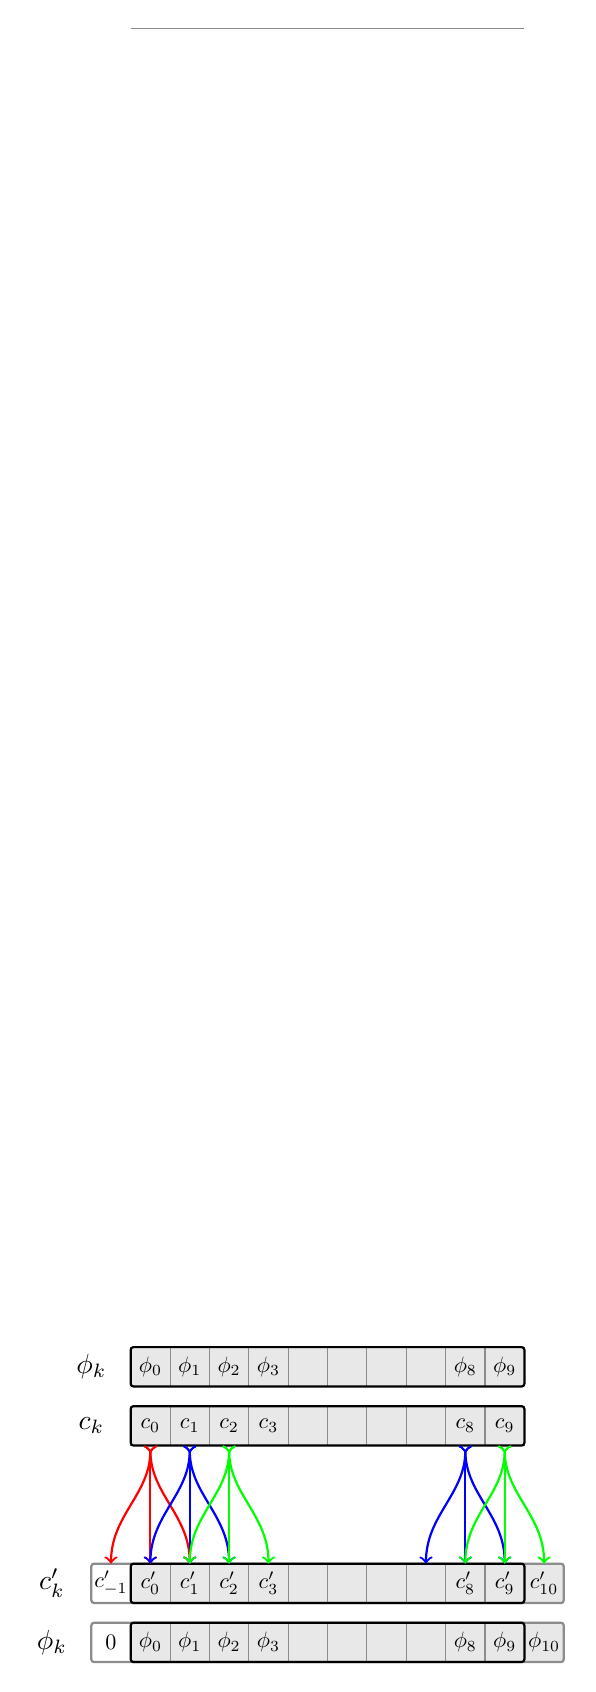
\begin{tikzpicture}
  \coordinate (co0) at (0.25, 2.0);
  \coordinate (co1) at (0.75, 2.0);
  \coordinate (co2) at (1.25, 2.0);
  \coordinate (co3) at (1.75, 2.0);
  \coordinate (co8) at (4.25, 2.0);
  \coordinate (co9) at (4.75, 2.0);

  \coordinate (cpm1) at (-0.25, 0.5);
  \coordinate (cp0) at (0.25, 0.5);
  \coordinate (cp1) at (0.75, 0.5);
  \coordinate (cp2) at (1.25, 0.5);
  \coordinate (cp3) at (1.75, 0.5);
  \coordinate (cp7) at (3.75, 0.5);
  \coordinate (cp8) at (4.25, 0.5);
  \coordinate (cp9) at (4.75, 0.5);
  \coordinate (cp10) at (5.25, 0.5);

  % upper
  \fill[gray!20, rounded corners=1] (0.0,2.0) rectangle (5.0,2.5);
  \draw[step=5mm, gray] (0,2.0) grid (5,2.5);
  \draw[black, thick, rounded corners=1] (0.0,2.0) rectangle (5.0,2.5);

  \fill[gray!20, rounded corners=1] (0.0,2.75) rectangle (5.0,3.25);
  \draw[step=5mm, ystep=20cm, gray] (0.0,2.75) grid (5.0,3.25);
  \draw[black, thick, rounded corners=1] (0.0,2.75) rectangle (5.0,3.25);

  % lower
  \fill[gray!20, rounded corners=1] (0.0,-0.75) rectangle (5.5,-0.25);
  \draw[step=5mm, ystep=20cm, gray] (0.0,-0.75) grid (5.0,-0.25);
  \draw[gray, thick, rounded corners=1] (-0.5,-0.75) rectangle (5.5,-0.25);
  \draw[black, thick, rounded corners=1] (0.0,-0.75) rectangle (5.0,-0.25);

  \fill[gray!20, rounded corners=1] (0.0,0.0) rectangle (5.5,0.5);
  \draw[step=5mm, gray] (0.0,0.0) grid (5.0,0.5);
  \draw[gray, thick, rounded corners=1] (-0.5,0.0) rectangle (5.5,0.5);
  \draw[black, thick, rounded corners=1] (0.0,0.0) rectangle (5.0,0.5);

  \draw[>->, thick, color=red] (co0) to[out=270,in=90] (cpm1);
  \draw[>->, thick, color=red] (co0) to[out=270,in=90] (cp0);
  \draw[>->, thick, color=red] (co0) to[out=270,in=90] (cp1);

  \draw[>->, thick, color=blue] (co1) to[out=270,in=90] (cp0);
  \draw[>->, thick, color=blue] (co1) to[out=270,in=90] (cp1);
  \draw[>->, thick, color=blue] (co1) to[out=270,in=90] (cp2);

  \draw[>->, thick, color=green] (co2) to[out=270,in=90] (cp1);
  \draw[>->, thick, color=green] (co2) to[out=270,in=90] (cp2);
  \draw[>->, thick, color=green] (co2) to[out=270,in=90] (cp3);

  \draw[>->, thick, color=blue] (co8) to[out=270,in=90] (cp7);
  \draw[>->, thick, color=blue] (co8) to[out=270,in=90] (cp8);
  \draw[>->, thick, color=blue] (co8) to[out=270,in=90] (cp9);

  \draw[>->, thick, color=green] (co9) to[out=270,in=90] (cp8);
  \draw[>->, thick, color=green] (co9) to[out=270,in=90] (cp9);
  \draw[>->, thick, color=green] (co9) to[out=270,in=90] (cp10);

  \node[scale=0.8] at (0.25,2.25) [black] {$c_0$};
  \node[scale=0.8] at (0.75,2.25) [black] {$c_1$};
  \node[scale=0.8] at (1.25,2.25) [black] {$c_2$};
  \node[scale=0.8] at (1.75,2.25) [black] {$c_3$};
  \node[scale=0.8] at (4.25,2.25) [black] {$c_8$};
  \node[scale=0.8] at (4.75,2.25) [black] {$c_9$};

  \node[scale=0.8] at (-0.25,0.25) [black] {$c^\prime_{-1}$};
  \node[scale=0.8] at (0.25,0.25) [black] {$c^\prime_0$};
  \node[scale=0.8] at (0.75,0.25) [black] {$c^\prime_1$};
  \node[scale=0.8] at (1.25,0.25) [black] {$c^\prime_2$};
  \node[scale=0.8] at (1.75,0.25) [black] {$c^\prime_3$};
  \node[scale=0.8] at (4.25,0.25) [black] {$c^\prime_8$};
  \node[scale=0.8] at (4.75,0.25) [black] {$c^\prime_9$};
  \node[scale=0.8] at (5.25,0.25) [black] {$c^\prime_{10}$};

  \node[scale=0.8] at (0.25,3.0) [black] {$\phi_0$};
  \node[scale=0.8] at (0.75,3.0) [black] {$\phi_1$};
  \node[scale=0.8] at (1.25,3.0) [black] {$\phi_2$};
  \node[scale=0.8] at (1.75,3.0) [black] {$\phi_3$};
  \node[scale=0.8] at (4.25,3.0) [black] {$\phi_8$};
  \node[scale=0.8] at (4.75,3.0) [black] {$\phi_9$};

  \node[scale=0.8] at (-0.25,-0.5) [black] {$0$};
  \node[scale=0.8] at (0.25,-0.5) [black] {$\phi_0$};
  \node[scale=0.8] at (0.75,-0.5) [black] {$\phi_1$};
  \node[scale=0.8] at (1.25,-0.5) [black] {$\phi_2$};
  \node[scale=0.8] at (1.75,-0.5) [black] {$\phi_3$};
  \node[scale=0.8] at (4.25,-0.5) [black] {$\phi_8$};
  \node[scale=0.8] at (4.75,-0.5) [black] {$\phi_9$};
  \node[scale=0.8] at (5.25,-0.5) [black] {$\phi_{10}$};

  \node at (-0.5,3.0) [black] {$\phi_{k}$};
  \node at (-1.0,-0.5) [black] {$\phi_{k}$};
  \node at (-0.5,2.25) [black] {$c_{k}$};
  \node at (-1.0,0.25) [black] {$c^\prime_{k}$};
\end{tikzpicture}

  \caption[Scatter-type stencil in 1D] {The scatter-type stencil application for
           computing the gradient $y\Phi$. The upper two arrays show the initial linear
           combination $\Phi$ consisting of basis functions $\phi_k$ and coefficients $c_k$.
           The lower two arrays show the linear combination of $\diff{\Phi}{x}$ consisting
           of the same basis functions $\phi_k$ and new coefficients $c_k^\prime$.
           Each of the triple arrows represents the computation for a fixed $\vec{k} \in \mathfrak{K}$
           (formula \eqref{eq:grad_basis_function_DD}), not all computations are shown.
           We see that the basis shape $\overline{\mathfrak{K}}$ for the gradient
           has to be larger. And also that we write to several elements not part
           of the original basis shape $\mathfrak{K}$. We drop the coefficient
           $c_{-1}^\prime$ (because $\phi_{-1} \equiv 0$).
           The original basis shape $\mathfrak{K}$ is represented by the black rectangle
           and the actual basis shapes are shown shaded grey.}
  \label{fig:grad_phi_kl_scatter_stencil_1D}
\end{figure}

\begin{figure}
  \centering
  \begin{tikzpicture}[scale=1,every node/.style={minimum size=0.5cm},on grid]

  \begin{scope}[
      yshift=-100,
      every node/.append style={yslant=0.5, xslant=-1.3},
      yslant=0.5,
      xslant=-1.3
    ]
    \coordinate (c32) at (1.75, 1.25);
    \coordinate (co25) at (1.25, 2.75);
  \end{scope}

  \begin{scope}[
      yshift=-160,
      every node/.append style={yslant=0.5, xslant=-1.3},
      yslant=0.5,
      xslant=-1.3
    ]
    \coordinate (cp42) at (2.25, 1.25);
    \coordinate (cp32) at (1.75, 1.25);
    \coordinate (cp22) at (1.25, 1.25);
    \coordinate (cp33) at (1.75, 1.75);
    \coordinate (cp31) at (1.75, 0.75);

    \coordinate (cop15) at (0.75, 2.75);
    \coordinate (cop25) at (1.25, 2.75);
    \coordinate (cop35) at (1.75, 2.75);
    \coordinate (cop24) at (1.25, 2.25);
    \coordinate (cop26) at (1.25, 3.25);
  \end{scope}

  % lower plane
  \begin{scope}[
      yshift=-160,
      every node/.append style={yslant=0.5, xslant=-1.3},
      yslant=0.5,
      xslant=-1.3
    ]
    \draw[step=5mm, thin, gray] (-0.5,-0.5) grid (3.5,3.5);

    \fill[blue!60] (2,1) rectangle (2.5,1.5);
    \node at (cp42) [draw, color=blue] {};%{$c^\prime_{4,2}$};

    \fill[blue!60] (1.5,1) rectangle (2.0,1.5);
    \node at (cp32) [draw, color=blue] {};%{$c^\prime_{3,2}$};

    \fill[blue!60] (1,1) rectangle (1.5,1.5);
    \node at (cp22) [draw, color=blue] {};%{$c^\prime_{2,2}$};

    \fill[blue!60] (1.5,1.5) rectangle (2.0,2.0);
    \node at (cp33) [draw, color=blue] {};%{$c^\prime_{3,3}$};

    \fill[blue!60] (1.5,0.5) rectangle (2.0,1.0);
    \node at (cp31) [draw, color=blue] {};%{$c^\prime_{3,1}$};

    \fill[orange!60] (0.5,2.5) rectangle (1.0,3.0);
    \node at (cop15) [draw, color=orange] {};%{$c^\prime_{1,5}$};

    \fill[orange!60] (1.0,2.5) rectangle (1.5,3.0);
    \node at (cop25) [draw, color=orange] {};%{$c^\prime_{2,5}$};

    \fill[orange!60] (1.5,2.5) rectangle (2.0,3.0);
    \node at (cop35) [draw, color=orange] {};%{$c^\prime_{3,5}$};

    \fill[orange!60] (1.0,2.0) rectangle (1.5,2.5);
    \node at (cop24) [draw, color=orange] {};%{$c^\prime_{2,4}$};

    \fill[orange!60] (1.0,3.0) rectangle (1.5,3.5);
    \node at (cop26) [draw, color=orange] {};%{$c^\prime_{2,6}$};

    \draw[black,thick, rounded corners=1] (0,0) rectangle (3,3);
    \draw[gray,thick, rounded corners=1] (-0.5,-0.5) rectangle (3.5,3.5);
  \end{scope}

  % arrows
  \begin{scope}
    \draw[>->, thick] (c32) node[left,scale=1.3] {} to[out=270,in=90] (cp42);
    \draw[>->, thick] (c32) node[left,scale=1.3] {} to[out=270,in=90] (cp32);
    \draw[>->, thick] (c32) node[left,scale=1.3] {} to[out=270,in=90] (cp22);
    \draw[>->, thick] (c32) node[left,scale=1.3] {} to[out=270,in=90] (cp33);
    \draw[>->, thick] (c32) node[left,scale=1.3] {} to[out=270,in=90] (cp31);

    \draw[>->, thick] (co25) node[left,scale=1.3] {} to[out=270,in=90] (cop24);
    \draw[>->, thick] (co25) node[left,scale=1.3] {} to[out=270,in=90] (cop25);
    \draw[>->, thick] (co25) node[left,scale=1.3] {} to[out=270,in=90] (cop26);
    \draw[>->, thick] (co25) node[left,scale=1.3] {} to[out=270,in=90] (cop15);
    \draw[>->, thick] (co25) node[left,scale=1.3] {} to[out=270,in=90] (cop35);
  \end{scope}

  % upper plane
  \begin{scope}[
      yshift=-100,
      every node/.append style={yslant=0.5, xslant=-1.3},
      yslant=0.5,
      xslant=-1.3
    ]
    \fill[white,fill opacity=0.8] (0,0) rectangle (3,3);
    \draw[step=5mm, thin, gray] (0,0) grid (3,3);

    \fill[blue!60] (1.5,1) rectangle (2.0,1.5);
    \node at (c32) [draw, color=blue] {};%{$c_{3,2}$};

    \fill[orange!60] (1.0,2.5) rectangle (1.5,3.0);
    \node at (co25) [draw, color=orange] {};%{$c_{2,5}$};

    \draw[black,thick, rounded corners=1] (0,0) rectangle (3,3);
  \end{scope}

  \node at (-3.25cm,-1.5cm) [black] {$c_{k,l}$};
  \node at (-4cm,-5.5cm) [black] {$\vec{c}^\prime_{k,l}$};
\end{tikzpicture}

  \caption[Scatter-type stencil in 2D] {The scatter-type stencil application for
           computing the gradient $y\Phi$. The upper array (plane) shows the
           coefficients $c_{\vec{k}}$ of the initial linear combination $\Phi(\vec{x})$.
           The lower array (plane) shows the coefficients $\vec{c}^\prime_{\vec{k}}$ of the
           linear combination of $\nabla\Phi(\vec{x})$ where each square is not a single
           number but stands for a whole vector. Each arrow bundle represents the
           computation for a fixed $\vec{k} \in \mathfrak{K}$ (formula
           \eqref{eq:grad_basis_function_DD}), not all computations are shown.
           The original basis shape $\mathfrak{K}$ is given by the black rectangle.
           We then see that the basis shape $\overline{\mathfrak{K}}$ for the gradient
           is larger by one square on each side. (But we again drop all coefficients
           with negative index.)
           The orange stencil shows that we sometimes have to write to elements
           (coefficients) that are not part of the original basis shape. Therefore
           we need to extend the basis shape where the whole lower plane stands
           for $\overline{\mathfrak{K}}$.
}
  \label{fig:grad_phi_kl_scatter_stencil_2D}
\end{figure}

\begin{algorithm}
\caption{Compute the gradient $y \Phi$ by scatter-type stencil application}
\label{al:grad_phi_scatter_type}
\begin{algorithmic}
  \REQUIRE Scalar wavepacket $\Phi$ in $D$ space dimensions
  \REQUIRE Basis shape $\mathfrak{K}$ (including linearisation mapping $\mu_{\mathfrak{K}}$) of $\Phi$
  \REQUIRE Parameters $\Pi$ and coefficients $\{c_{\vec{k}}\}$ of $\Phi$

  \STATE // Extend the basis shape $\mathfrak{K}$
  \STATE $\overline{\mathfrak{K}} \assign \text{\bf{extend\_basis\_shape}}(\mathfrak{K})$

  \STATE // Storage space for the result
  \STATE $\mat{c}^\prime = \mat{0} \in \mathbb{C}^{D \times |\overline{\mathfrak{K}}|}$

  \STATE // Iterate over original basis shape
  \FOR{$\vec{k} \in \mathfrak{K}$}

    \STATE // Central node
    \STATE $\mat{c}^\prime[:,\mu_{\overline{\mathfrak{K}}}(\vec{k})] =
            \mat{c}^\prime[:,\mu_{\overline{\mathfrak{K}}}(\vec{k})] +
            c_{\vec{k}} \, \vec{p}$

    \STATE // Backward neighbours
    \FOR{$d = 0$ \TO $d = D-1$}
      \STATE $\vec{k}^\prime = \vec{k} - \vec{e}^d$
      \IF{$\vec{k}^\prime \in \overline{\mathfrak{K}}$}
        \STATE $\mat{c}^\prime[:,\mu_{\overline{\mathfrak{K}}}(\vec{k}^\prime)] =
                \mat{c}^\prime[:,\mu_{\overline{\mathfrak{K}}}(\vec{k}^\prime)] +
                \sqrt{\frac{\varepsilon^2}{2}} \sqrt{\vec{k}[d]} \, c_{\vec{k}} \, \conj{\mat{P}}[:,d]$
      \ENDIF
    \ENDFOR

    \STATE // Forward neighbours
    \FOR{$d = 0$ \TO $d = D-1$}
      \STATE $\vec{k}^\prime = \vec{k} + \vec{e}^d$
      \IF{$\vec{k}^\prime \in \overline{\mathfrak{K}}$}
        \STATE $\mat{c}^\prime[:,\mu_{\overline{\mathfrak{K}}}(\vec{k}^\prime)] =
                \mat{c}^\prime[:,\mu_{\overline{\mathfrak{K}}}(\vec{k}^\prime)] +
                \sqrt{\frac{\varepsilon^2}{2}} \sqrt{\vec{k}[d]+1} \, c_{\vec{k}} \, \mat{P}[:,d]$
      \ENDIF
    \ENDFOR

  \ENDFOR
  \RETURN $\overline{\mathfrak{K}}$ and $\mat{c}^\prime$
\end{algorithmic}
\end{algorithm}


\subsection{An example}


As an example we take a wavepacket $\Ket{\Psi}$ in two space dimensions with the
following parameter set $\Pi = \{\vec{0}, \vec{0}, \id, i \id \}$ and $\varepsilon = 0.6$.
The coefficients are set to the values printed in the next table.

\begin{center}
\begin{tabular}{l r}
$\vec{k}$ & $c_{\vec{k}}$ \\
\hline
$(0,0)$ & $0.5$ \\
$(0,1)$ & $0.5$ \\
$(1,1)$ & $0.5$ \\
$(2,1)$ & $0.5$
\end{tabular}
\end{center}

A plot of the wavepacket evaluated on a small region of position space is shown
in figure \ref{fig:wavepacket_original}.

\begin{figure}
  \centering
  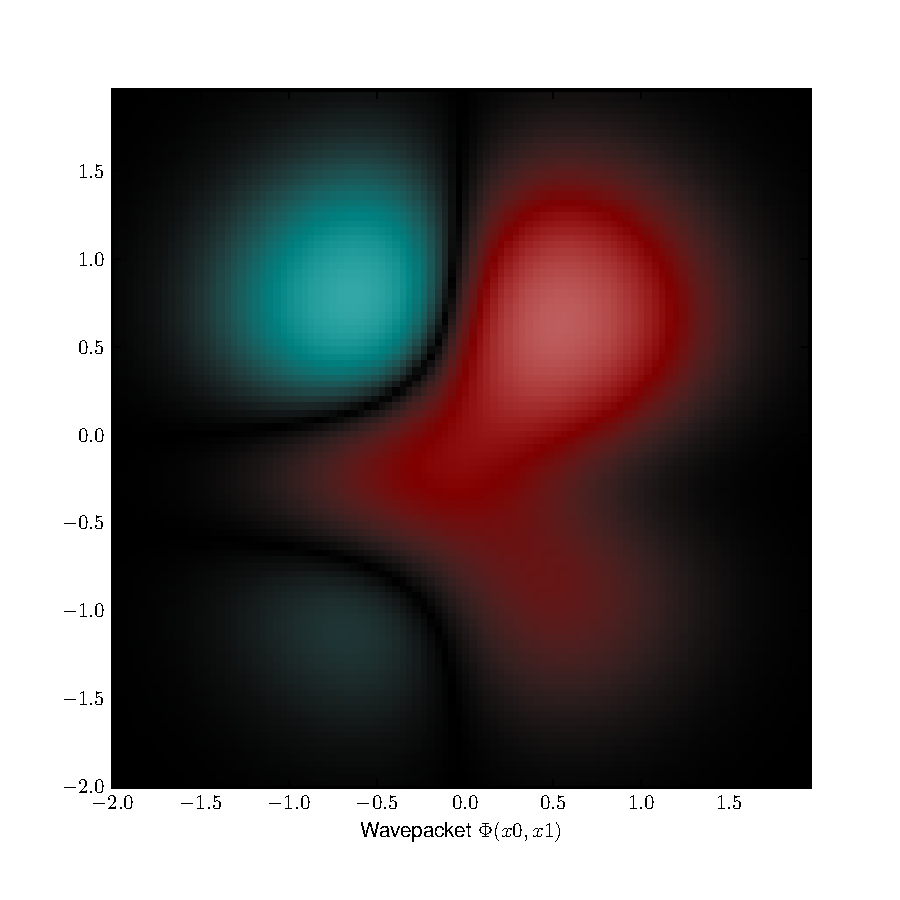
\includegraphics[scale=0.3]{./fig/wavepacket_original.pdf}
  \caption[Wavepacket of the gradient example]{The wavepacket $\Ket{\Psi}$.}
  \label{fig:wavepacket_original}
\end{figure}

Next we compute the gradient $-i \varepsilon \nabla \Psi$ by one of the above
methods. For the new coefficients $\vec{c}_{\vec{k}}$ we get the values (only
non-zero ones) shown in the next table. The two components of the gradient
are plotted in figure \ref{fig:wavepacket_gradient}.

\begin{center}
\begin{tabular}{l r r}
$\vec{k}$ & $x_0$ component of $\vec{c}_{\vec{k}}$ &  $x_1$ component of $\vec{c}_{\vec{k}}$ \\
\hline
$(0,0)$ &$0$                            & $- 0.21213203 \mathbf{\imath}$ \\
$(0,1)$ &$- 0.21213203 \mathbf{\imath}$ & $0.21213203 \mathbf{\imath}$ \\
$(1,0)$ &$0.21213203 \mathbf{\imath}$   & $- 0.21213203 \mathbf{\imath}$ \\
$(1,1)$ &$- 0.08786797 \mathbf{\imath}$ & $0$  \\
$(2,0)$ &$0$                            & $- 0.21213203 \mathbf{\imath}$ \\
$(2,1)$ &$0.3 \mathbf{\imath}$          & $0$  \\
$(3,1)$ &$0.36742346 \mathbf{\imath}$   & $0$  \\
$(0,2)$ &$0$                            & $0.3 \mathbf{\imath}$ \\
$(1,2)$ &$0$                            & $0.3 \mathbf{\imath}$ \\
$(2,2)$ &$0$                            & $0.3 \mathbf{\imath}$ \\
\end{tabular}

\end{center}\begin{figure}
  \centering
  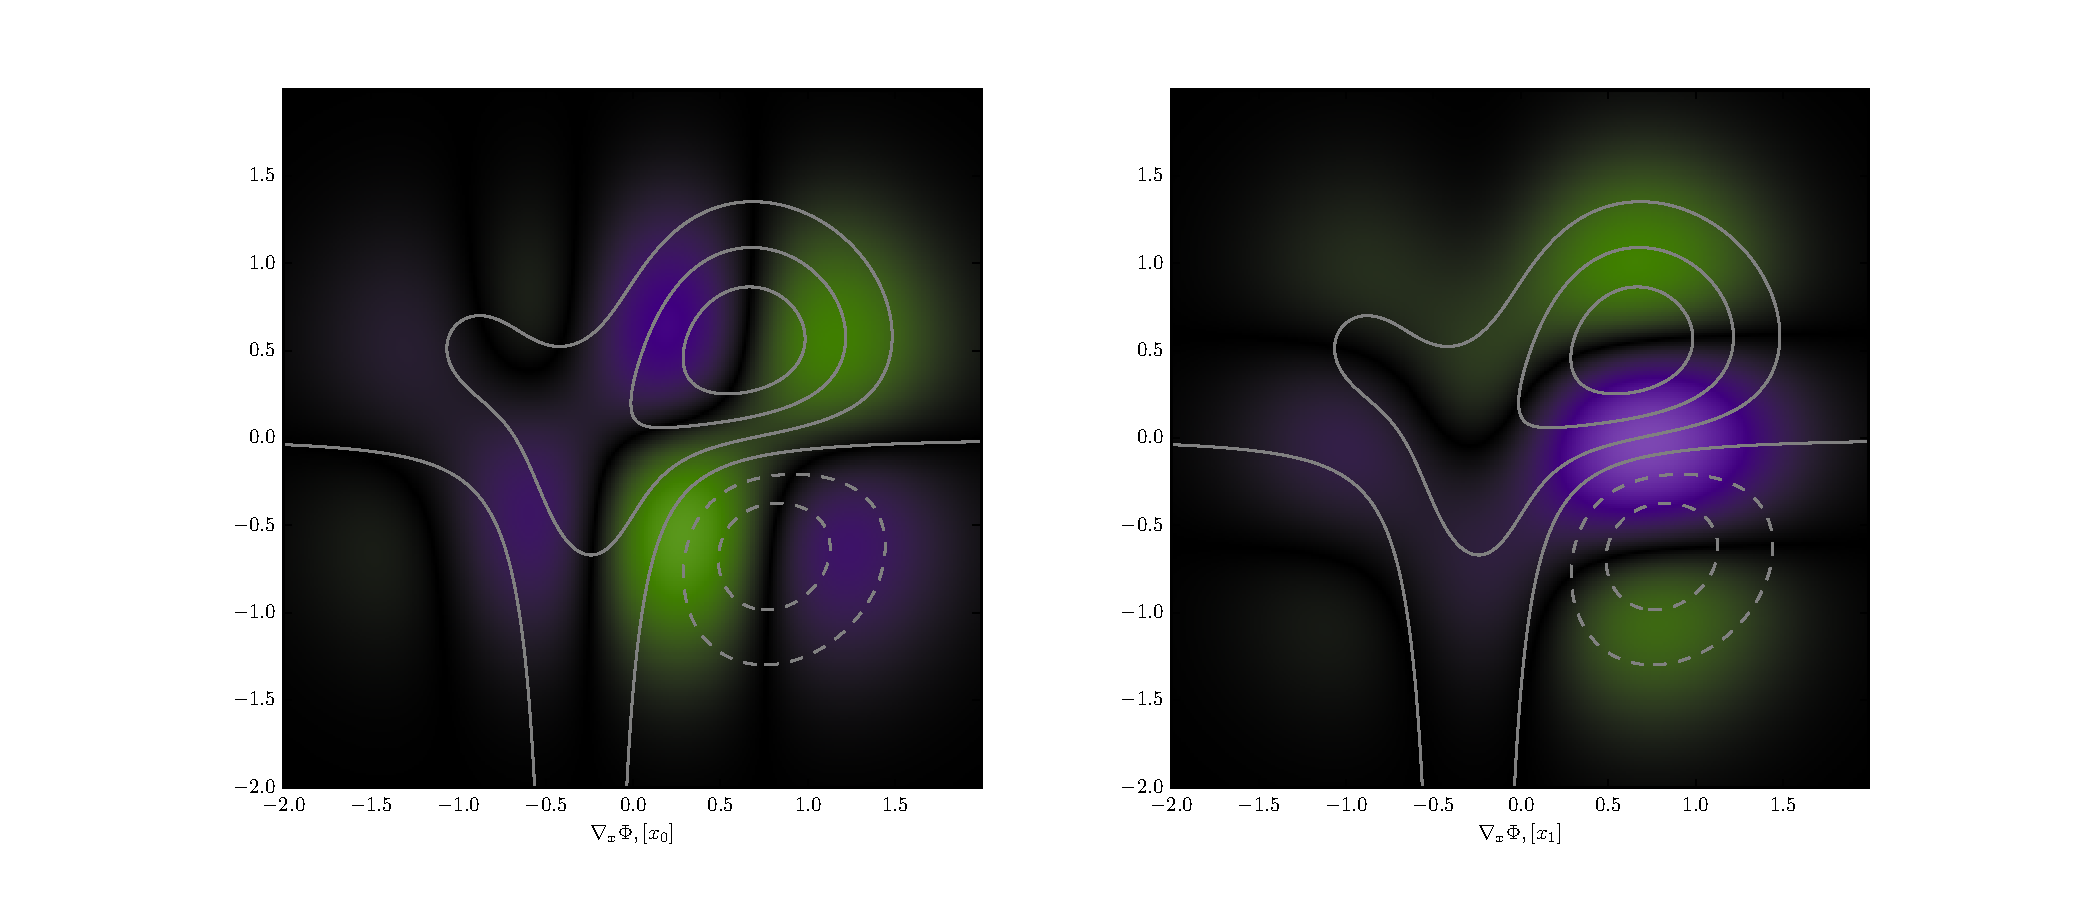
\includegraphics[scale=0.32]{./fig/wavepacket_gradient.pdf}
  \caption[Plots of the gradient example]
          {The $x_0$ (left) and $x_1$ (right) components of the gradient
           $-i \varepsilon \nabla \Psi$. The wavepacket $\Psi$ is indicated
           by some contour levels just for reference.}
  \label{fig:wavepacket_gradient}
\end{figure}

Finally, figure \ref{fig:wavepacket_coefficients} shows again the coefficients
of both, the original wavepacket and the two components of its gradient.

\begin{figure}
  \centering
  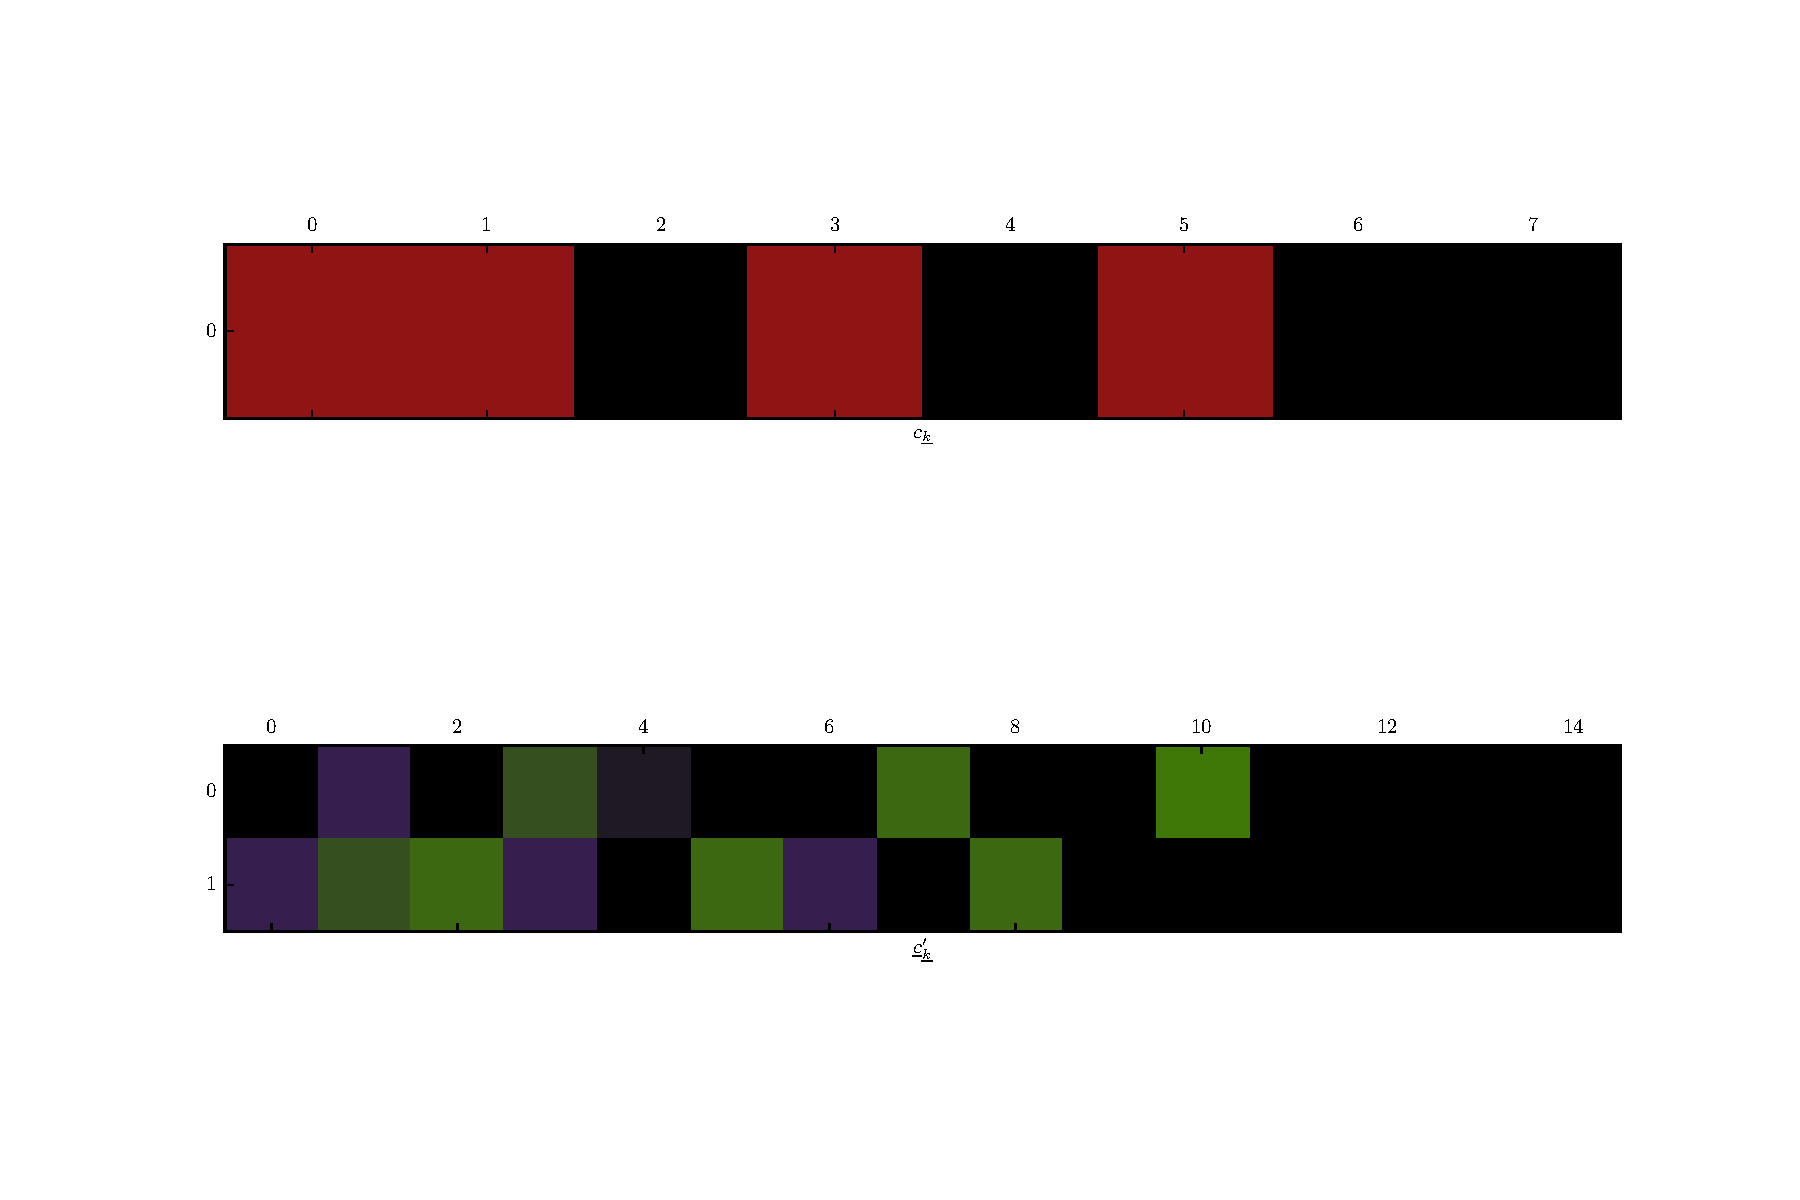
\includegraphics[width=0.8\linewidth]{./fig/wavepacket_coefficients.pdf}
  \caption[Coefficients of the gradient example]
         {Coefficients $c_{\vec{k}}$ of $\Psi$ (top) and $\vec{c}_{\vec{k}}$ of
          $-i \varepsilon \nabla \Psi$ (bottom). Notice also the different basis
          sizes $|\mathfrak{K}|$ of 8 and 15.}
  \label{fig:wavepacket_coefficients}
\end{figure}


\clearemptydoublepage

\begin{chapter}{Inner products, integrals and quadrature}
\label{ch:quadrature}

\section{A hierarchy of brakets}

In this chapter we will develop and summarize all necessary tools related to
inner products of wavepackets. We will follow a top down approach and start with
the braket of a full vector valued wavepacket $\Ket{\Psi}$ which may be homogeneous
or inhomogeneous at the moment. The primes indicate that the bra and the ket can
have different parameter sets $\Pi$. This is obvious when $\Ket{\Psi}$ is an
inhomogeneous wavepacket. Also we include an operator $F$ which may be the identity.

\begin{equation}
\begin{split}
  \Braket{\Psi | F | \Psi^\prime} & =
    \Bra{
    \begin{pmatrix}
    \Phi_0     \\
    \vdots     \\
    \Phi_{N-1}
    \end{pmatrix}
    }
    \begin{pmatrix}
    {}     & \vdots  & {} \\
    \hdots & F_{r,c} & {} \\
    {}     &         & {}
    \end{pmatrix}
    \Ket{
    \begin{pmatrix}
    \Phi_0^\prime     \\
    \vdots     \\
    \Phi_{N-1}^\prime
    \end{pmatrix}
    } \\
  & = \sum_{r=0}^{N-1} \sum_{c=0}^{N-1} \Braket{\Phi_r | F_{r,c} | \Phi_c^\prime}
\end{split}
\end{equation}

where $F$ is a $N \times N$ block matrix consisting of $K \times K$ blocks
denoted by $F_{i,j} \rassign f$. We then consider a single term out of this
double sum

\begin{equation}
\begin{split}
  \Braket{\Phi_i | f | \Phi_j^\prime} & =
    \Bra{
    \begin{pmatrix}
    \phi_0     \\
    \vdots     \\
    \phi_{K-1}
    \end{pmatrix}
    }
    \begin{pmatrix}
    {}     & \vdots  & {} \\
    \hdots & f_{k,l} & {} \\
    {}     &         & {}
    \end{pmatrix}
    \Ket{
    \begin{pmatrix}
    \phi_0^\prime     \\
    \vdots     \\
    \phi_{K-1}^\prime
    \end{pmatrix}
    } \\
  & = \sum_{k=0}^{K-1} \sum_{l=0}^{K-1} \Braket{\phi_k | f_{k,l} | \phi_l^\prime}
\end{split}
\end{equation}

where $\phi_i$ are the basis functions from \eqref{eq:hagedorn_kstate_1d}. Now we
pick again a single entry out of the double sum only and find the following
integral at the bottom of this hierarchy

\begin{equation} \label{eq:single_entry_braket}
  \Braket{\phi_k | f_{k,l} | \phi_l^\prime} = \int f_{k,l}\ofs{x} \conj{\phi_k\ofs{x}} \phi_l^\prime\ofs{x} \,.
\end{equation}

We now want to find an efficient way to calculate this integral for all $i$, $j$, $k$ and $l$
or, in other words, set up the matrix $F$. This integral can almost never be solved
analytically thus the integral is approximated by high order quadrature.


\section{Inner products of basis functions}

We speak of inhomogeneous inner products if the part in the bra and the part in
the ket of \eqref{eq:single_entry_braket} have different Hagedorn parameters sets $\Pi$.
In this case, all formulae become much more complicated.

\subsection{An analytical ansatz to inner products}

The inner product of two basis functions which have different sets of
parameters denoted by $\Pi_k \assign \{P_k, Q_k, S_k, p_k, q_k\}$ and
$\Pi_l \assign \{P_l, Q_l, S_l, p_l, q_l\}$ respectively is written as usual as
$\Braket{ \phi^k | \phi^l }$. This is the expression we want to evaluate now and
we can even write down a closed form solution based on induction and the recursion
relation for Hermite polynomials. The expression for the ground states $\phi_0$
acts as induction base and is given by

\begin{multline} \label{eq:multifamily_innerp_ground}
  \Braket{ \phi_0^k | \phi_0^l } =
  \sqrt{\frac{-2 i}{Q_2 \conj{P_1} - P_2 \conj{Q_1}}} \cdot
    \exp \Biggl(
      \frac{i}{2 \varepsilon^2}
      \frac{Q_2 \conj{Q_1} \left(p_2-p_1\right)^2 + P_2 \conj{P_1} \left(q_2-q_1\right)^2}
            {\left(Q_2 \conj{P_1} - P_2 \conj{Q_1}\right)}
    \\
    -\frac{i}{\varepsilon^2}
    \frac{\left(q_2-q_1\right) \left( Q_2 \conj{P_1} p_2 - P_2 \conj{Q_1} p_1\right)}
         {\left(Q_2 \conj{P_1} - P_2 \conj{Q_1}\right)}
    \Biggr) \,.
\end{multline}

For the inner product of higher level functions $\phi_i$ the whole thing gets much
more complicated

\begin{multline} \label{eq:mixing_braket}
  \Braket{ \phi_k^k | \phi_l^l } =
  \frac{1}{\sqrt{k!l!}} 2^{-\frac{k+l}{2}} \Braket{ \phi_0^k | \phi_0^l } \cdot
  \left(i \conj{ P_1} Q_2 - i \conj{Q_1} P_2\right)^{-\frac{k+l}{2}} \cdot \\
  \sum_{j=0}^{\min\left(k,l\right)}
    \Biggl(
      \binom{k}{j} \binom{l}{j} j! 4^j
      \left(i Q_2  P_1 - i Q_1  P_2\right)^{\frac{k-j}{2}}
      \left(i \conj{Q_2 P_1} - i\conj{Q_1 P_2}\right)^{\frac{l-j}{2}}
      \\
      \cdot H_{k-j}\left(-\frac{1}{\varepsilon}
                    \frac{Q_2\left(p_1-p_2\right)-P_2\left(q_1-q_2\right)}
                         {\sqrt{Q_2 P_1 - Q_1 P_2}\sqrt{\conj{P_1}Q_2-\conj{Q_1} P_2}}\right)
      \\
      \cdot H_{l-j}\left(\frac{1}{\varepsilon}
                   \frac{\conj{ P_1}\left(q_1-q_2\right)-\conj{Q_1}\left(p_1-p_2\right)}
                        {\sqrt{\conj{Q_2 P_1}-\conj{Q_1 P_2}}\sqrt{\conj{ P_1}Q_2-\conj{Q_1} P_2}}\right)
    \Biggr) \,.
\end{multline}

For the proofs of these formulae see reference \cite{H_R_quantization_rules}.

Despite we can evaluate the inner product and have a closed form solution for arbitrary
wavefunctions, these formulae are unsuitable for numerical calculation. There are
several reasons but for example the factorials and binomial coefficients lead to
overflow even for relatively small $k$ and $l$. Further the sum may be numerically
unstable. Thus we need to find a better way to perform these calculations.


\subsection{Inhomogeneous or mixing quadrature rule}
\label{sec:mixing_quadrature}

In this section we will develop a quadrature rule to evaluate the brakets in \eqref{eq:mixing_braket}.
First we notice that each $\phi$ which is given by \eqref{eq:hagedorn_kstate_1d}
is represented through a mathematical expression of the general form

\begin{equation} \label{eq:expression_format}
  C \cdot P^n\ofs{\xi} \cdot \exp \ofs{\theta}
\end{equation}

consisting of an arbitrary constant $C \in \mathbb{C}$, a polynomial $P^n\ofs{\cdot}$
of degree $n$ and an exponential $\exp\ofs{\cdot}$. We try a new ansatz for calculating
the inner product. Evaluating the braket $\Braket{\phi^k | \phi^l}$ results in a
multiplication of two expressions of the form \eqref{eq:expression_format}. The
parts in this expression can be grouped by same type

\begin{equation} \label{eq:expression_reformat}
\begin{split}
  \Braket{\phi^k | \phi^l} & =
  \int_\mathbb{R} \conj{C_k P^n_k\ofs{\xi_k} \exp \ofs{\theta_k}} C_l P^n_l\ofs{\xi_l} \exp \ofs{\theta_l} \,dx \\
  & =   \int_\mathbb{R} \conj{C_k} C_l P^n_k\ofs{\conj{\xi_k}} P^n_l\ofs{\xi_l} \exp \ofs{\conj{\theta_k}} \exp \ofs{\theta_l} \,dx \,.
\end{split}
\end{equation}

Let's take a closer look at the integrand of this expression now. With Gauss Hermite
quadrature in mind we are especially interested in the exponential parts. They have
a general form like

\begin{equation} \label{eq:expression_format_exponential}
  \exp\ofs{\theta} = \exp\left(s \cdot \left(x-m\right)^2 + \cdots \right) \,.
\end{equation}

We concentrate on the exponentials of \eqref{eq:expression_reformat} only. We combine
them and distribute the complex conjugate onto the variables affected

\begin{equation*}
\begin{split}
    & \conj{\exp\left(\frac{i}{2\varepsilon^2} P_k Q_k^{-1} \left(x-q_k\right)^2 + \frac{i}{\varepsilon^2} p_k \left( x-q_k \right)\right)}
      \cdot \exp\left(\frac{i}{2\varepsilon^2} P_l Q_l^{-1} \left(x-q_l\right)^2 + \frac{i}{\varepsilon^2} p_l \left( x-q_l \right)\right) \\
  = & \exp\left(\conj{\frac{i}{2\varepsilon^2} P_k Q_k^{-1} \left(x-q_k\right)^2 + \frac{i}{\varepsilon^2} p_k \left( x-q_k \right)}
              + \frac{i}{2\varepsilon^2} P_l Q_l^{-1} \left(x-q_l\right)^2 + \frac{i}{\varepsilon^2} p_l \left( x-q_l \right) \right) \\
  = & \exp\left( -\frac{i}{2\varepsilon^2} \conj{P_k} \conj{Q_k^{-1}} \left(x-q_k\right)^2 - \frac{i}{\varepsilon^2} p_k \left( x-q_k \right)
              + \frac{i}{2\varepsilon^2} P_l Q_l^{-1} \left(x-q_l\right)^2 + \frac{i}{\varepsilon^2} p_l \left( x-q_l \right) \right) \,.
\end{split}
\end{equation*}

For the sake of readability we define the following variables

\begin{equation}
\begin{split}
  r_k & \assign P_k Q_k^{-1} \\
  r_l & \assign P_l Q_l^{-1} \,.
\end{split}
\end{equation}

Plugging these into the equation above and expanding the squares we get for the
exponent

\begin{equation*}
  \frac{i}{\varepsilon^2} \left( - \frac{1}{2}\underbrace{\left(\conj{r_k}-r_l\right)}_{\alpha + i \beta} x^2
                                 + \underbrace{\left(\conj{r_k}q_k-r_l q_l\right)}_{\gamma + i \delta} x
                                 - \underbrace{\frac{1}{2}\left(\conj{r_k}q_k^2 + r_l q_l^2\right)
                                 + \left(p_l-p_k\right) x
                                 + p_k q_k - p_l q_l}_{\text{junk}}
                          \right)
\end{equation*}

where we introduced two new complex variables $\alpha + i \beta$ and $\gamma + i \delta$
and sorted out some unimportant expressions. We now carry out the multiplication
with respect to the real parts of these complex numbers. This yields

\begin{equation}
  -\frac{1}{\varepsilon^2} \left( -\frac{\beta}{2}x^2 + i \left(\cdots\right)
                                  + \delta x -i \left(\cdots\right)
                                  + \cdots
                          \right)
\end{equation}

where the dots indicate more junk. To get back to a form along the lines of
\eqref{eq:expression_format_exponential} we have to complete the square, first
divide out a factor of $-\frac{\beta}{2}$ and then complete by a factor of
$\left(\frac{\delta}{\beta}\right)^2$

\begin{equation}
\begin{split}
    & -\frac{1}{\varepsilon^2} \left( x^2 -\frac{2\delta}{\beta} x + \ldots \right) \left(-\frac{\beta}{2}\right) \\
%   = & -\frac{1}{\varepsilon^2} \left( x^2 -\frac{2\delta}{\beta} x + \left(\frac{\delta}{\beta}\right)^2 - \left(\frac{\delta}{\beta}\right)^2 \right) \left(-\frac{\beta}{2}\right) \\
%   = & -\frac{1}{\varepsilon^2} \left( \left(-\frac{\beta}{2}\right) \left(x-\frac{\delta}{\beta}\right)^2 - \left(-\frac{\beta}{2}\right)\left(\frac{\delta}{\beta}\right)^2 \right) \\
  = & -\frac{1}{\varepsilon^2} \left( \left(-\frac{\beta}{2}\right) \left(x-\frac{\delta}{\beta}\right)^2 + \frac{\delta^2}{2\beta} \right) \,.
\end{split}
\end{equation}

From this last expression we get the quadrature rule components $s \assign Q_0$
and $m \assign q_0$ of expression \eqref{eq:expression_format_exponential} as

\begin{equation} \label{eq:inhomog_quad_params}
\begin{split}
  q_0 & \assign \frac{\delta}{\beta} = \frac{\Im \left(\conj{r_k}q_k-r_l q_l\right)}{\Im \left(\conj{r_k}-r_l\right)} \\
  Q_0 & \assign -\frac{\beta}{2} = -\frac{\Im \left(\conj{r_k}-r_l\right)}{2} \\
  Q_S & \assign \frac{1}{\sqrt{Q_0}} \,.
\end{split}
\end{equation}

Now we transform the nodes $\gamma_i$ according to the weighted position mean $q_0$
and the parameter $Q_S$ which changes the spread of the nodes. This yields

\begin{equation} \label{eq:inhomog_transformed_nodes}
  \gamma^{\prime}_i \assign q_0 + \varepsilon \cdot Q_S \cdot \gamma_i
\end{equation}

for the mixing quadrature nodes which are located in the space around where
the product of $\phi_k$ and $\phi_l$ is maximal. A procedure that calculates
$q_0$, $Q_S$ and the adapted quadrature nodes is given by algorithm \ref{al:mixing_hagedorn_parameters}.

\begin{algorithm}
\caption{Mixing two sets $\Pi_r$ and $\Pi_c$ of Hagedorn parameters}
\label{al:mixing_hagedorn_parameters}
\begin{algorithmic}
  \REQUIRE Two sets $\Pi_r$ and $\Pi_c$ of Hagedorn parameters
  \REQUIRE A quadrature rule $\left(\gamma_i, \omega_i\right)$
  \STATE // Apply the mixing formula to the parameters
  \STATE $r_r \assign \frac{P_r}{Q_r}$
  \STATE $r_c \assign \frac{P_c}{Q_c}$

  \STATE $q_0 \assign \frac{\Im \left(\conj{r_r}q_r-r_c q_c\right)}{\Im \left(\conj{r_r}-r_c\right)}$
  \STATE $Q_0 \assign -\frac{\Im \left(\conj{r_r}-r_c\right)}{2}$
  \STATE $Q_S \assign \frac{1}{\sqrt{Q_0}}$

  \STATE // And shift the quadrature nodes
  \STATE $\gamma^\prime \assign q_0 + \varepsilon Q_S \gamma$
  \RETURN $q_0$ and $Q_S$ and $\gamma^\prime$
\end{algorithmic}
\end{algorithm}

We get back to the homogeneous case if we choose the sets $\Pi_k$ and
$\Pi_l$ of Hagedorn parameters identical.

Note that we get issues if at any time it happens that

\begin{equation}
  \Im \left(\frac{\conj{P_k}}{\conj{Q_k}} -\frac{P_l}{Q_l}\right) > 0 \,.
\end{equation}


\subsection{Homogeneous quadrature rule}

In this section we reduce the mixing quadrature rule of the last section to the
homogeneous case where everything becomes much simpler.
We will start from the assumption that the mixing quadrature rule contains the
homogeneous one as a special case. (This is not just speculation but can be shown
by direct calculation analogous to what we did in the last section.) Suppose for
this section that both $\phi_i$ in \eqref{eq:single_entry_braket} belong to the
same basis and have an identical parameter set $\Pi$ hence $\Pi_k = \Pi_l$ or at
least $P_k = P_l$, $Q_k = Q_l$ and $p_k = p_l$, $q_k = q_l$. With this assumption
we simplify the quadrature formulae \eqref{eq:inhomog_quad_params} and
\eqref{eq:inhomog_transformed_nodes} to the homogeneous case.

Let's start with simplification of the $Q_0$ parameter

\begin{equation}
\begin{split}
  Q_0 & \assign -\frac{\Im \left(\conj{r_k}-r_l\right)}{2}
        = -\frac{1}{2} \Im \left(\conj{r_k}-r_k\right) \\
      & = - \frac{1}{2} \left( - \frac{2}{\conj{Q}Q}\right) \\
      & = \frac{1}{|Q|^2} \,.
\end{split}
\end{equation}

The parameter $Q_S$ is then as trivial as

\begin{equation}
  Q_S \assign \frac{1}{\sqrt{Q_0}} = \frac{1}{\sqrt{\frac{1}{|Q|^2}}} = |Q| \,.
\end{equation}

In the last case we have for the weighted position

\begin{equation}
\begin{split}
  q_0 & \assign \frac{\Im \left(\conj{r_k}q_k-r_l q_l\right)}{\Im \left(\conj{r_k}-r_l\right)}
        = \frac{\Im \left(\conj{r_k}q_k-r_k q_k\right)}{\Im \left(\conj{r_k}-r_k\right)} \\
%       & = \frac{\Im \left(\left(\conj{r_k}-r_k\right) q\right)}{-\frac{2}{\conj{Q}Q}}
      & = \frac{q \Im \left(\conj{r_k}-r_k\right)}{-\frac{2}{\conj{Q}Q}}
        = \frac{-\frac{2}{\conj{Q}Q}q}{-\frac{2}{\conj{Q}Q}} \\
      & = q
\end{split}
\end{equation}

which should be clear also without computation. For the transformed quadrature
nodes we can write

\begin{equation}
  \gamma^{\prime}_i \assign q + \varepsilon \cdot |Q| \cdot \gamma_i
\end{equation}

which was shown to work in real simulations for homogeneous wavepackets.


% \subsubsection{Direct computation}
%
% The above result is consistent with what we get directly from the following computations
% starting with the already simplified exponentials. Just for comparison here is the
% direct derivation of the homogeneous quadrature rule.
%
% \begin{align} \label{eq:expression_exponentials_combined}
%   & \conj{\exp\left(\frac{i}{2\varepsilon^2} P Q^{-1} \left(x-q\right)^2 + \frac{i}{\varepsilon^2} p \left( x-q \right)\right)}
%   \cdot \exp\left(\frac{i}{2\varepsilon^2} P Q^{-1} \left(x-q\right)^2 + \frac{i}{\varepsilon^2} p \left( x-q \right)\right) \nonumber \\
%   = & \exp\left(\conj{\frac{i}{2\varepsilon^2} P Q^{-1} \left(x-q\right)^2 + \frac{i}{\varepsilon^2} p \left( x-q \right)}
%               + \frac{i}{2\varepsilon^2} P Q^{-1} \left(x-q\right)^2 + \frac{i}{\varepsilon^2} p \left( x-q \right) \right) \nonumber \\
%   = & \exp\left( -\frac{i}{2\varepsilon^2} \conj{P} \conj{Q^{-1}} \left(x-q\right)^2 - \frac{i}{\varepsilon^2} p \left( x-q \right)
%               + \frac{i}{2\varepsilon^2} P Q^{-1} \left(x-q\right)^2 + \frac{i}{\varepsilon^2} p \left( x-q \right) \right) \,.
% \end{align}
%
% Now we group the terms with an $x^2$ but without expanding the binomals. Thus we get
%
% \begin{align}
%     & -\frac{i}{2\varepsilon^2} \conj{P} \conj{Q^{-1}} \left(x-q\right)^2 + \frac{i}{2\varepsilon^2} P Q^{-1} \left(x-q\right)^2 - \frac{i}{\varepsilon^2} p \left( x-q \right)
%                + \frac{i}{\varepsilon^2} p \left( x-q \right) \\
%   = & -\frac{i}{2\varepsilon^2} \conj{P} \conj{Q^{-1}} \left(x-q\right)^2 + \frac{i}{2\varepsilon^2} P Q^{-1} \left(x-q\right)^2 + \bigO{x} \\
%   = & \frac{i}{\varepsilon^2} \left( -\frac{1}{2} \conj{P} \conj{Q^{-1}} \left(x-q\right)^2 + \frac{1}{2} P Q^{-1} \left(x-q\right)^2 \right) + \ldots \\
%   = & \frac{i}{\varepsilon^2} \left( \left(-\frac{1}{2} \conj{P} \conj{Q^{-1}} + \frac{1}{2} P Q^{-1} \right) \left(x-q\right)^2 \right) + \ldots \\
%   = & \frac{i}{\varepsilon^2} \left( -\frac{1}{2} \underbrace{\left( \frac{\conj{P}}{\conj{Q}} - \frac{P}{Q} \right)}_{\text{*}} \left(x-q\right)^2 \right) + \ldots \\
%   = & \frac{i}{\varepsilon^2} \left( -\frac{1}{2} \left( -2i \frac{1}{\conj{Q}Q} \right) \left(x-q\right)^2 \right) + \ldots \\
%   = & -\frac{1}{\varepsilon^2} \left( \frac{1}{\conj{Q}Q} \left(x-q\right)^2 \right) + \ldots \\
%   = & -\frac{1}{\varepsilon^2} \left( \underbrace{\frac{1}{|Q|^2}}_{Q_0} \left(x-\underbrace{q}_{q_0}\right)^2 \right) + \ldots \\
% \end{align}
%
% from which we again get for the quadrature nodes
%
% \begin{equation}
%   \gamma^{\prime}_i \assign q + \varepsilon \cdot |Q| \cdot \gamma_i
% \end{equation}


\section{Quadrature rules applied}

After we discussed in details the transformation of the quadrature nodes in the
last section we now look at the final quadrature rule. It's not really difficult,
but it is good to write down all the details at least once.

Assume we have the transformed quadrature nodes $\gamma_i^\prime$ given by \eqref{eq:inhomog_transformed_nodes}.
We now carry out the quadrature for resolving equation \eqref{eq:single_entry_braket}

\begin{equation}
\begin{split}
  \Braket{\phi_k | f | \phi_l^\prime}
  \approx
  \varepsilon \cdot Q_S \cdot \sum_{r=0}^R \conj{\phi_k\ofs{\gamma_r^\prime}} \cdot f\ofs{\gamma_r^\prime} \cdot \phi_l^\prime\ofs{\gamma_r^\prime} \cdot \omega_r
\end{split}
\end{equation}

where the two $\phi$ in general belong to the different families. But if they really
have the same parameter sets $\Pi$ then we can simplify this formula slightly. The
trick is that we omit a prefactor of $\frac{1}{\sqrt{Q}}$ when evaluating $\phi\ofs{\gamma_r^\prime}$.
Because we have two times this evaluation, both prefactors accumulate to $\frac{1}{|Q|}$.
In the homogeneous case we have $Q_S = |Q|$ hence the $Q_S$ outside the sum
cancels nicely with this prefactors. And the above formula becomes

\begin{equation} \label{eq:homogeneous_quadrature_rule}
\begin{split}
  \Braket{\phi_k | f | \phi_l}
  \approx
  \varepsilon \cdot \sum_{r=0}^R \conj{\phi_k\ofs{\gamma_r^\prime}} \cdot f\ofs{\gamma_r^\prime} \cdot \phi_l\ofs{\gamma_r^\prime} \cdot \omega_r \,.
\end{split}
\end{equation}

\end{chapter}


\clearemptydoublepage

\begin{chapter}{Motivation and procedure for spawning wavepackets}
\label{ch:spawnprocedure}

In this chapter we will review the important parts from the paper about tunneling
dynamics and spawning \cite{GHJ_tunneling_spawning}. This is necessary because all
the further chapters about spawning of wavepackets in the non-adiabatic case build
upon and generalize the basic ideas developed there. Also we will work out the basic
mathematical procedure for spawning new wavepackets.


\section{The tunneling problem}

In tunneling dynamics we consider a potential shaped like a steep hill. The so
called Eckart potential, defined as $V\ofs{x} \assign \frac{v_0}{\cosh^2 \ofs{a x}}$
where $v_0$ is the potential energy at the maximum and $a$ is another constant,
serves as a good example of such a potential. This potential is shown in figure
\ref{fig:eckart_potential} for later reference.

\begin{figure}
  \centering
  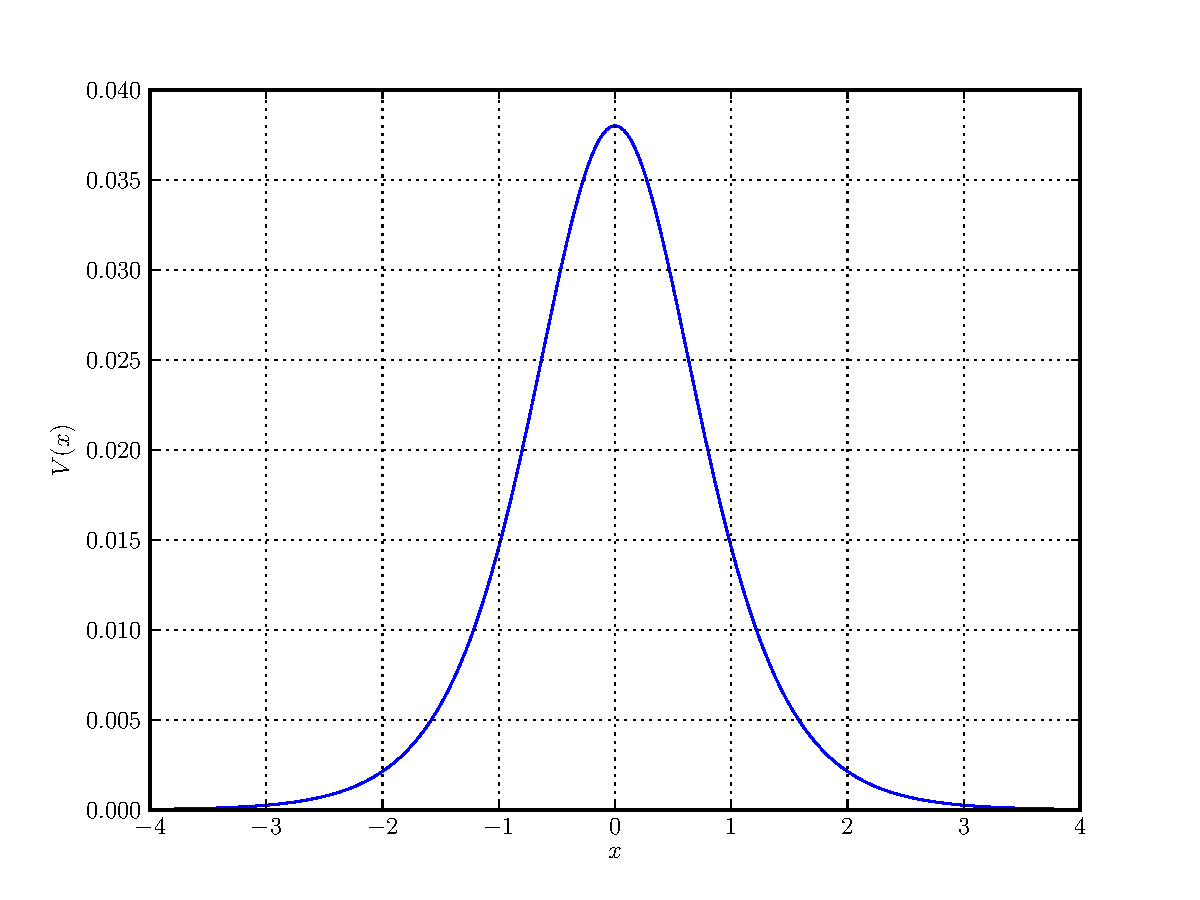
\includegraphics[scale=0.4]{./figures/eckart.pdf}
  \caption[The Eckart potential]{The Eckart potential with the parameters set to $v_0 = 0.038008$ and
  $a = 1.05836$ (same values as in ref.\cite{GHJ_tunneling_spawning}).}
  \label{fig:eckart_potential}
\end{figure}

Suppose now that we have a particle coming from one side and moving towards the
potential. In the classical world, the particle either crosses over the hill or
gets reflected depending on its momentum only. In the quantum world however, the
wavefunction always splits up in two parts of which one will be reflected and the
other transmitted. These two parts usually have very different amplitudes and will
drift apart more and more while their interaction rapidly becomes negligible as
they are separated by the potential hill.

\subsection{Motivation for spawning}

For our algorithm based on wavepackets as defined in chapter \ref{ch:wavepackets}
this split becomes problematical. The reason is that we need very high frequencies
to represent the tunneled part of our wavepacket. In most settings the energy of
the wavepacket is strictly smaller than the peak value of the potential. This implies
that during the propagation of the parameter set $\Pi$ the parameter $q$ which
centers the basis functions $\phi_k$ in position space gets reflected at the
potential. Therefore we get a good basis for representing the reflected part (with
only very few basis functions). This basis obviously is unsuitable for representing
the tunneled part and indeed we need many basis functions in the high frequency
domain. (These problems wouldn't matter if we worked with a infinite basis.)

In figure \ref{fig:tunneling_highfreq} the output of a tunneling simulation using
wavepackets is shown at late time. We clearly see the issue explained above. A basis
of size about $20$ would be sufficient for representing the reflected part accurately.
But for the transmitted part we need up to about $250$ basis functions. And the
problem gets worse with time (slowly) requiring more and more basis functions. Another important
point to notice is that there is a range of coefficients with negligible values in
the middle. In the example this range extends roughly from $40$ to $110$.

From this observation it's self-evident that breaking up the packet into two independent
parts would be a good idea. This then would also allow us to represent each packet
with a much smaller basis. And in the case of tunneling we could even neglect the
interaction between the two packets without loosing much information.

\begin{figure}
  \centering
  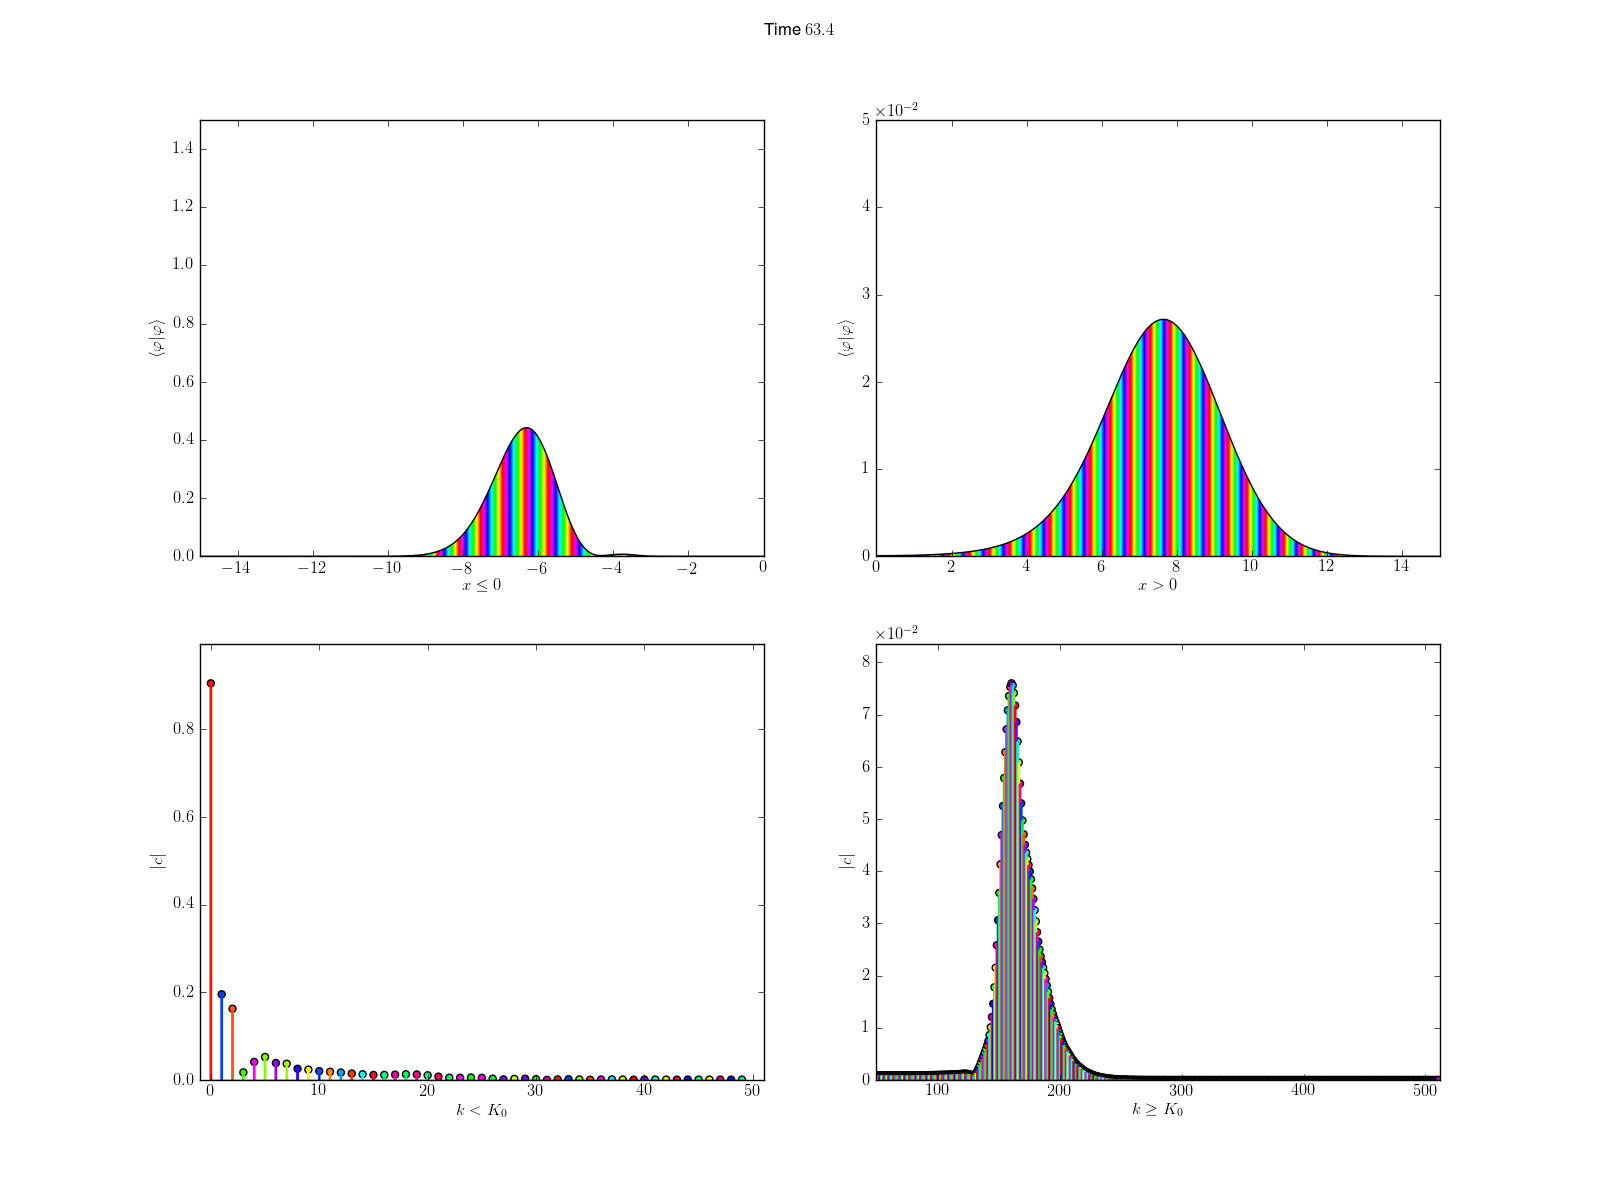
\includegraphics[width=\linewidth]{./figures/spawn_reason.png}
  \caption[Tunneling simulation example motivating the spawning approach]
  {This figure shows the output of a tunneling simulation at late time.
  The upper two panels show $\Braket{\Phi|\Phi}$ for the wavepacket $\Ket{\Phi}$.
  The lower two panels show the absolute value $|c_k|$ of the coefficients. The colors
  represent the complex phase according to the convention from \cite{Thaller_VQM}.
  Please notice the different scales! For the upper panels the $x$ axis is split
  at $0$ and the $y$ axes have a sensible scale. In the lower left panel we have
  the coefficients for $k < 50$ while the values for $k \geq 50$ are in the right
  panel where again the $y$ axis is scaled appropriately.}
  \label{fig:tunneling_highfreq}
\end{figure}


\section{Spawning a new packet}

With the motivation from the last section we will now investigate the steps that
have to be taken for spawning a new wavepacket. A first step is to find a new,
suitable basis. Remember that for fixed $\varepsilon$ the set of functions
$\{\phi_k\}_{k=0}^K$ gives a complete (but truncated) basis of the space $L^2$
and this is all we need for expanding our wavepacket into a linear combination.
Finding this basis is depicted in great detail in section \ref{sec:parameter_estimation}.
Although the mathematics behind this process is mostly trivial, there are plenty
of opportunities to make mistakes. Given this new basis we need to find a method
for transferring (a part of) the wavepacket to this new basis. We describe two
basically different methods in section \ref{sec:change_of_basis}.

\section{Parameter estimation}
\label{sec:parameter_estimation}

\subsection{Fragments}

In the remainder of this chapter we will use a so called \emph{fragment} $\Ket{w}$ as a
kind of a placeholder. The definition is very similar to the one of a full scalar
wavepacket $\Ket{\Phi}$ but more flexible for our purpose of lying out the basic
formalism for spawning wavepackets. So we define our fragment as

\begin{equation} \label{eq:def_fragment}
  \Ket{w} \assign \sum_{k=\alpha}^\beta c_k \phi_k
\end{equation}

with $\alpha, \beta \in \mathbb{N}_0$ and $\beta \geq \alpha$. Basically this is
just a handy abbreviation for an arbitrary linear combination of several basis functions.
If we demand that $\alpha,\beta \in \left[0, K-1\right]$ it becomes clear why we
call this a fragment, compared to the full (scalar) wavepacket in \eqref{eq:hawp_def_single}.
And in the case of $\alpha=0$ and $\beta=K-1$ we recover the full packet by

\begin{equation}
  \Ket{\Phi} = \exp\ofs{\frac{iS}{\varepsilon^2}} \Ket{w} \,.
\end{equation}

In principle the fragment could be sparse but this is mathematically equivalent
to saying that $\exists k \in \left[\alpha, \ldots, \beta\right] : c_k = 0$ and
thus we do not care further.

For the moment it does not matter what $w$ precisely is, all we need to know about
it is given by equation \eqref{eq:def_fragment}. Later $w$ may be a fully normalized
wavepacket $\Phi = \sum_{k=0}^{K-1} c_k \phi_k$, only a part of a wavepacket
$\Phi^\prime = \sum_{k=\alpha}^{\beta} c_k \phi_k$ with $\alpha \geq 0$ and
$\beta \leq K-1$ or a single component $\Phi_i = \sum_{k=0}^{K-1} c_k^i \phi_k^i$
of a homogeneous or inhomogeneous vector valued wavepacket $\Psi$ depending
on the context where the spawning technique is to be applied.  In the example
shown in figure \eqref{fig:tunneling_highfreq} motivating this chapter, $w$ would
be what is shown in the right column.

As said above the first step is to find a new (in some measure \emph{better})
basis $\{\tilde{\phi}_k\}_{k=0}^\infty$ of the space $L^2$ for representing $\Ket{w}$.
The basis functions $\tilde{\phi}_k$ are fully characterized by the parameter set
$\tilde{\Pi} \assign \{\tilde{P},\tilde{Q},\tilde{p},\tilde{q}\}$ so all we have
to do is estimate these four values. By the way, we denote all quantities in the
new bases with a tilde. The new position $\tilde{q}$ and new momentum $\tilde{p}$
are both real numbers and therefore easy. So we will handle these two first to
get a feeling for the procedure.


\subsection{Position $\tilde{q}$ and Momentum $\tilde{p}$}

The parameters $\tilde{q}$ and $\tilde{p}$ can be interpreted as the average position
and momentum. For this reason we compute expectation values of the position and momentum
operators

\begin{align}
  \tilde{q} & \assign \frac{\Braket{w | x | w}}{\Braket{w|w}} \\
  \tilde{p} & \assign \frac{\Braket{w | y | w}}{\Braket{w|w}}
\end{align}

where we divide by $\Braket{w|w}$ since the fragment is not normalized in general.
We can get an explicit expression for position operator $x$ and the momentum
operator $y$ by solving the linear system consisting of the definitions of both
ladder operators as shown in \eqref{eq:definition_ladder_ops} and get

\begin{equation}
\label{eq:definition_pos_and_mom_ops}
\begin{split}
  x \assign & \sqrt{\frac{\varepsilon^2}{2}} \left(Q \mathcal{R} + \conj{Q} \mathcal{L}\right) + q \\
  y \assign & \sqrt{\frac{\varepsilon^2}{2}} \left(P \mathcal{R} + \conj{P} \mathcal{L}\right) + p \,.
\end{split}
\end{equation}

Notice the symmetry in the two operators. We can transform $x$ into $y$ by the two
replacements $Q \rightarrow P$ and $q \rightarrow p$. This will halve the work
when calculating properties of these operators.

Starting with a fragment $\Ket{w}$ and an arbitrary operator $O$ and expanding the
linear combination we arrive at a double sum over brakets including basis functions
$\phi_k$ only

\begin{equation}
\label{eq:operator_expectation}
\begin{split}
  \Braket{w | O | w} \assign & \Braket{\sum_{k=\alpha}^\beta c_k \phi_k | O | \sum_{l=\alpha}^\beta c_l \phi_l} \\
                            = & \sum_{k=\alpha}^{\beta} \sum_{l=\alpha}^{\beta} \conj{c_k} c_l \Braket{\phi_k | O | \phi_l} \,.
\end{split}
\end{equation}

Now we have to see what happens with these simpler brakets. The full calculation
for the position operator $x$ works as follows where we use sesquilinearity and the
properties of the ladder operators

\begin{equation*}
\begin{split}
  \Braket{\phi_k | x | \phi_l}
  \assign & \Braket{\phi_k | \sqrt{\frac{\varepsilon^2}{2}} \left(Q \mathcal{R} + \conj{Q} \mathcal{L}\right) + q | \phi_l} \\
  = & \Braket{\phi_k | \sqrt{\frac{\varepsilon^2}{2}} Q \mathcal{R} | \phi_l}
    + \Braket{\phi_k | \sqrt{\frac{\varepsilon^2}{2}} \conj{Q} \mathcal{L} | \phi_l}
    + \Braket{\phi_k | q | \phi_l} \\
  = & \sqrt{\frac{\varepsilon^2}{2}} Q \Braket{\phi_k | \mathcal{R} | \phi_l}
    + \sqrt{\frac{\varepsilon^2}{2}} \conj{Q} \Braket{\phi_k | \mathcal{L} | \phi_l}
    + q \Braket{\phi_k | \phi_l} \\
  = & \sqrt{\frac{\varepsilon^2}{2}} Q \Braket{\phi_k | \sqrt{l+1} \phi_{l+1}}
    + \sqrt{\frac{\varepsilon^2}{2}} \conj{Q} \Braket{\phi_k | \sqrt{l} \phi_{l-1}}
    + q \Braket{\phi_k | \phi_l}
\end{split}
\end{equation*}

and finally we get

\begin{equation}
  \label{eq:estimate_pos_basis}
  \Braket{\phi_k | x | \phi_l}
  = \sqrt{\frac{\varepsilon^2}{2}} \left( Q \sqrt{l+1} \Braket{\phi_k | \phi_{l+1}}
    + \conj{Q} \sqrt{l} \Braket{\phi_k | \phi_{l-1}} \right)
    + q \Braket{\phi_k | \phi_l} \,.
\end{equation}

Applying the symmetry mentioned above we get a similar formula for the momentum
operator

\begin{equation}
  \label{eq:estimate_mom_basis}
  \Braket{\phi_k | y | \phi_l}
  = \sqrt{\frac{\varepsilon^2}{2}} \left( P \sqrt{l+1} \Braket{\phi_k | \phi_{l+1}}
    + \conj{P} \sqrt{l} \Braket{\phi_k | \phi_{l-1}} \right)
    + p \Braket{\phi_k | \phi_l} \,.
\end{equation}

Using the orthonormality of the basis function we can write

\begin{align}
  \Braket{\phi_k | x | \phi_l}
  & = \sqrt{\frac{\varepsilon^2}{2}} \left( Q \sqrt{l+1} \kron{k,l+1}
    + \conj{Q} \sqrt{l} \kron{k,l-1} \right)
    + q \kron{k,l} \\
  \Braket{\phi_k | y | \phi_l}
  & = \sqrt{\frac{\varepsilon^2}{2}} \left( P \sqrt{l+1} \kron{k,l+1}
    + \conj{P} \sqrt{l} \kron{k,l-1} \right)
    + p \kron{k,l} \,.
\end{align}

At this point we can substitute back these expressions into the double sum from
\eqref{eq:operator_expectation} which then gives

\begin{equation*}
\begin{split}
  \Braket{w | x | w} = & \sum_{k=\alpha}^\beta \sum_{l=\alpha}^\beta \conj{c_k} c_l
                         \left( \sqrt{\frac{\varepsilon^2}{2}} \left( Q \sqrt{l+1} \kron{k,l+1}
                         + \conj{Q} \sqrt{l} \kron{k,l-1} \right) + q \kron{k,l} \right) \\
  = &   \sum_{k=\alpha}^\beta \sum_{l=\alpha}^\beta \conj{c_k} c_l \sqrt{\frac{\varepsilon^2}{2}} Q \sqrt{l+1} \kron{k,l+1}
      + \sum_{k=\alpha}^\beta \sum_{l=\alpha}^\beta \conj{c_k} c_l \sqrt{\frac{\varepsilon^2}{2}} \conj{Q} \sqrt{l} \kron{k,l-1} \\
    & + \sum_{k=\alpha}^\beta \sum_{l=\alpha}^\beta \conj{c_k} c_l q \kron{k,l} \,.
\end{split}
\end{equation*}

Because of the Kronecker deltae each of these three double sums can be reduced
to a single sum only. For the first one we have $\kron{k,l+1} = 1 \iff l = k-1$
thus

\begin{equation} \label{eq:part1}
  \sum_{k=\alpha}^\beta \sum_{l=\alpha}^\beta \conj{c_k} c_l \sqrt{\frac{\varepsilon^2}{2}} Q \sqrt{l+1} \kron{k,l+1}
  = \sqrt{\frac{\varepsilon^2}{2}} Q \sum_{k=\alpha+1}^\beta \conj{c_k} c_{k-1} \sqrt{k} \,.
\end{equation}

See also figure \ref{fig:sumgrid} for a better overview over these nasty index transformations.
For the second sum the relation is $\kron{k,l-1} = 1 \iff l = k+1$ and therefore

\begin{equation} \label{eq:part2}
  \sum_{k=\alpha}^\beta \sum_{l=\alpha}^\beta \conj{c_k} c_l \sqrt{\frac{\varepsilon^2}{2}} \conj{Q} \sqrt{l} \kron{k,l-1}
  = \sqrt{\frac{\varepsilon^2}{2}} \conj{Q} \sum_{k=\alpha}^{\beta-1} \conj{c_k} c_{k+1} \sqrt{k+1} \,.
\end{equation}

The third one is trivial as $\kron{k,l} = 1 \iff l=k$ and we find

\begin{equation}
  \sum_{k=\alpha}^\beta \sum_{l=\alpha}^\beta \conj{c_k} c_l q \kron{k,l} = q \sum_{k=\alpha}^\beta \conj{c_k} c_k \,.
\end{equation}

Notice that this sum is nothing else than the norm of $w$.
We can simplify the expression for $\Braket{w|x|w}$ further. For this we first shift
the summation index of the right hand side of \eqref{eq:part2} up by one. (Equivalently
we could also shift down the index of \eqref{eq:part1} by one.) Mathematically this means
that $k^\prime = k+1$ which gives $k = k^\prime -1$ and we find that

\begin{equation} \label{eq:part2s}
  \sqrt{\frac{\varepsilon^2}{2}} \conj{Q} \sum_{k=\alpha}^{\beta-1} \conj{c_k} c_{k+1} \sqrt{k+1}
  = \sqrt{\frac{\varepsilon^2}{2}} \conj{Q} \sum_{k^\prime=\alpha+1}^{\beta} \conj{c_{k^\prime-1}} c_{k^\prime} \sqrt{k^\prime}
\end{equation}

where we wrote the primes once for clarity and drop them from now on. Recognizing
now that \eqref{eq:part1} and \eqref{eq:part2s} are complex conjugates of each other
we can combine them and write for the whole expression

\begin{align}
  \Braket{w|x|w}
  & = \sqrt{\frac{\varepsilon^2}{2}} Q \sum_{k=\alpha+1}^\beta \conj{c_k} c_{k-1} \sqrt{k}
    + \sqrt{\frac{\varepsilon^2}{2}} \conj{Q} \sum_{k=\alpha+1}^{\beta} \conj{c_{k-1}} c_{k} \sqrt{k}
    + q \sum_{k=\alpha}^\beta \conj{c_k} c_k \nonumber \\
  & = \sqrt{2 \varepsilon^2} \Re \left(Q \sum_{k=\alpha+1}^\beta \conj{c_k} c_{k-1} \sqrt{k} \right)
    + q \sum_{k=\alpha}^\beta \conj{c_k} c_k \,.
\end{align}

The very same procedure can be applied for the momentum operator $y$ too, but of
course we take the shortcut by symmetry and get

\begin{equation}
  \Braket{w|y|w}
  = \sqrt{2 \varepsilon^2} \Re \left(P \sum_{k=\alpha+1}^\beta \conj{c_k} c_{k-1} \sqrt{k} \right)
  + p \sum_{k=\alpha}^\beta \conj{c_k} c_k \,.
\end{equation}

If we now remember that the fragment may not be normalized we find the final formulae
for the expected position and momentum of $w$

\begin{align}
  \tilde{q} & \assign \frac{\Braket{w | x | w}}{\Braket{w|w}}
            = \frac{\sqrt{2 \varepsilon^2}}{\sum_{k=\alpha}^\beta \conj{c_k} c_k} \Re \left(Q \sum_{k=\alpha+1}^\beta \conj{c_k} c_{k-1} \sqrt{k} \right) + q 
            \label{eq:estimate_pos} \\
  \tilde{p} & \assign \frac{\Braket{w | y | w}}{\Braket{w|w}}
            = \frac{\sqrt{2 \varepsilon^2}}{\sum_{k=\alpha}^\beta \conj{c_k} c_k} \Re \left(P \sum_{k=\alpha+1}^\beta \conj{c_k} c_{k-1} \sqrt{k} \right) + p \,.
            \label{eq:estimate_mom}
\end{align}

\begin{figure}
  \centering
  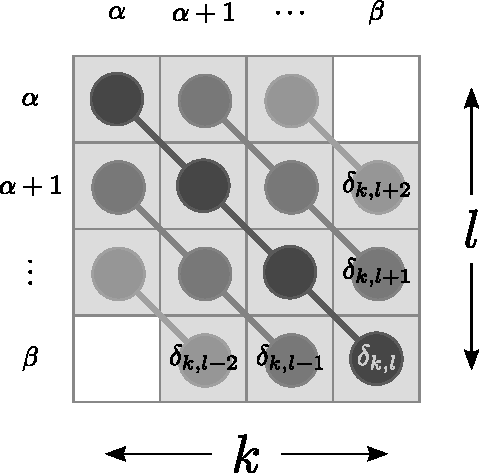
\includegraphics{./figures/sumgrid.pdf}
  \caption[Symbolic view on the double sum]{Symbolic view on the double sum
  $\sum_{k=\alpha}^\beta \sum_{l=\alpha}^\beta$. The diagonal lines show which
  elements remain in a single sum $\sum_k$ after expanding the corresponding
  Kronecker delta.}
  \label{fig:sumgrid}
\end{figure}

\subsection{Estimating second central moments}

In order to estimate the parameters $\tilde{Q}$ and $\tilde{P}$ of a fragment $w$
in a first step we have to compute the following two expectation values

\begin{equation} \label{eq:est_second_moments_def}
  \frac{\Braket{w | \left(x-\tilde{q}\right)^2 | w}}{\Braket{w|w}}
  \qquad \text{and} \qquad
  \frac{\Braket{w | \left(x-\tilde{p}\right)^2 | w}}{\Braket{w|w}}  
\end{equation}

which is in principle straight forward but very tedious. The reason why we compute
these quantities will become clear later but we essentially try to estimate second
central moments. We now show the whole procedure for the first braket and then use
the symmetry argument again to get the second one too. We start with expanding the
operator $\left(x-\tilde{q}\right)^2$ and break the expression into parts

\begin{equation} \label{eq:est_second_moment_pos}
\begin{split}
  \frac{\Braket{w | \left(x-\tilde{q}\right)^2 | w}}{\Braket{w|w}}
  & = \frac{\Braket{w | x^2 - 2 \tilde{q} x + \tilde{q}^2 | w}}{\Braket{w|w}} \\
  & = \frac{\Braket{w | x^2 | w}}{\Braket{w|w}}
    - 2 \tilde{q} \frac{\Braket{w | x | w}}{\Braket{w|w}}
    + \tilde{q}^2 \,.
\end{split}
\end{equation}

In the third term, the norms of $w$ cancel and we rediscover \eqref{eq:estimate_pos}
in  the second term. Thus all that is left over is

\begin{equation} \label{eq:est_second_moment_simplified}
  \frac{\Braket{w | \left(x-\tilde{q}\right)^2 | w}}{\Braket{w|w}}
  = \frac{\Braket{w | x^2 | w}}{\Braket{w|w}} - \tilde{q}^2 \,.
\end{equation}

Now we will concentrate on the first term and we have to struggle quite a bit to
compute it's numerator. As usual we decompose this braket by using the sesquilinearity
and write

\begin{equation} \label{eq:braket_basis_x2}
\begin{split}
  \Braket{w | x^2 | w}
  & = \Braket{\sum_{k=\alpha}^\beta c_k \phi_k | x^2 | \sum_{l=\alpha}^\beta c_l \phi_l} \\
  & = \sum_{k=\alpha}^\beta \sum_{l=\alpha}^\beta \conj{c_k} c_l \Braket{\phi_k | x^2 | \phi_l} \,.
\end{split}
\end{equation}

This reduced the problem to brakets over basis functions. At that point we need an
explicit version of the operator $x^2$ in terms of raising and lowering operators
which can be obtained as follows

\begin{equation} \label{eq:def_operator_x2}
\begin{split}
  x^2 & = \left(\sqrt{\frac{\varepsilon^2}{2}} \left(Q \mathcal{R} + \conj{Q} \mathcal{L}\right) + q\right)
          \left(\sqrt{\frac{\varepsilon^2}{2}} \left(Q \mathcal{R} + \conj{Q} \mathcal{L}\right) + q\right) \\
      & = \left( \theta Q \mathcal{R} + \theta \conj{Q} \mathcal{L} + q\right)
          \left( \theta Q \mathcal{R} + \theta \conj{Q} \mathcal{L} + q\right) \\
      & = \theta^2 Q\mathcal{R}Q\mathcal{R} + \theta^2Q\mathcal{R}\conj{Q}\mathcal{L}
        + \theta Q\mathcal{R}q + \theta^2 \conj{Q}\mathcal{L}Q\mathcal{R} + \theta^2\conj{Q}\mathcal{L}\conj{Q}\mathcal{L}
        + \theta \conj{Q}\mathcal{L}q + \theta qQ\mathcal{R} + \theta q \conj{Q}\mathcal{L} + q^2 \\
      & = \theta^2 Q^2 \mathcal{R}^2 + \theta^2 \conj{Q}^2 \mathcal{L}^2
        + \theta^2 Q\conj{Q} \mathcal{RL} + \theta^2 \conj{Q}Q \mathcal{LR}
        + 2\theta q Q \mathcal{R} + 2\theta q\conj{Q} \mathcal{L} + q^2
\end{split}
\end{equation}

where for simplicity we defined $\theta \assign \sqrt{\frac{\varepsilon^2}{2}}$.
We can now use the sesquilinearity of the inner product and split \eqref{eq:braket_basis_x2}
once more

\begin{align*}
  \Braket{\phi_k | x^2 | \phi_l} = & 
  \Braket{\phi_k | \theta^2 Q^2 \mathcal{R}^2 | \phi_l}
  +\Braket{\phi_k | \theta^2 \conj{Q}^2 \mathcal{L}^2 | \phi_l} \\
  & +\Braket{\phi_k | \theta^2 Q\conj{Q} \mathcal{RL} | \phi_l}
  +\Braket{\phi_k | \theta^2 \conj{Q}Q \mathcal{LR} | \phi_l} \\
  & +\Braket{\phi_k | 2\theta q Q \mathcal{R} | \phi_l}
  +\Braket{\phi_k | 2\theta q\conj{Q} \mathcal{L} | \phi_l}
  +\Braket{\phi_k | q^2 | \phi_l}
\end{align*}

resulting in seven parts which we will work out one after the other now. This is
a very boring task but necessary to justify the final relatively simple formula.

\begin{equation*}
\begin{split}
  \Braket{\phi_k | \theta^2 Q^2 \mathcal{R}^2 | \phi_l} & = \theta^2 Q^2 \Braket{\phi_k | \mathcal{R}^2 | \phi_l} \\
  & = \theta^2 Q^2 \Braket{\phi_k | \mathcal{R} | \sqrt{l+1} \phi_{l+1}} \\
  & = \theta^2 Q^2 \sqrt{l+1} \Braket{\phi_k | \sqrt{l+2} \phi_{l+2}} \\
  & = \theta^2 Q^2 \sqrt{l+1} \sqrt{l+2} \Braket{\phi_k | \phi_{l+2}}
    = \theta^2 Q^2 \sqrt{l+1} \sqrt{l+2} \kron{k,l+2}
\end{split}
\end{equation*}

\begin{equation*}
\begin{split}
  \Braket{\phi_k | \theta^2 \conj{Q}^2 \mathcal{L}^2 | \phi_l} & = \theta^2 \conj{Q}^2 \Braket{\phi_k | \mathcal{L}^2 | \phi_l} \\
  & = \theta^2 \conj{Q}^2 \Braket{\phi_k | \mathcal{L} | \sqrt{l} \phi_{l-1}} \\
  & = \theta^2 \conj{Q}^2 \sqrt{l} \Braket{\phi_k | \sqrt{l-1} \phi_{l-2}} \\
  & = \theta^2 \conj{Q}^2 \sqrt{l} \sqrt{l-1} \Braket{\phi_k | \phi_{l-2}}
    = \theta^2 \conj{Q}^2 \sqrt{l} \sqrt{l-1} \kron{k,l-2}
\end{split}
\end{equation*}

\begin{equation*}
\begin{split}
  \Braket{\phi_k | \theta^2 Q\conj{Q} \mathcal{RL} | \phi_l} & = \theta^2 Q\conj{Q} \Braket{\phi_k | \mathcal{RL} | \phi_l} \\
  & = \theta^2 Q\conj{Q} \Braket{\phi_k | \mathcal{R} | \sqrt{l} \phi_{l-1}} \\
  & = \theta^2 Q\conj{Q} \sqrt{l} \Braket{\phi_k | \sqrt{l} \phi_{l}} \\
  & = \theta^2 Q\conj{Q} l \Braket{\phi_k | \phi_{l}}
    = \theta^2 Q\conj{Q} l \kron{k,l}
\end{split}
\end{equation*}

\begin{equation*}
\begin{split}
  \Braket{\phi_k | \theta^2 \conj{Q}Q \mathcal{LR} | \phi_l} & = \theta^2 \conj{Q}Q \Braket{\phi_k | \mathcal{LR} | \phi_l} \\
  & = \theta^2 \conj{Q}Q \Braket{\phi_k | \mathcal{R} | \sqrt{l+1} \phi_{l+1}} \\
  & = \theta^2 \conj{Q}Q \sqrt{l+1} \Braket{\phi_k | \sqrt{l+1} \phi_{l}} \\
  & = \theta^2 \conj{Q}Q \left(l+1\right) \Braket{\phi_k | \phi_{l}}
    = \theta^2 \conj{Q}Q \left(l+1\right) \kron{k,l}
\end{split}
\end{equation*}

\begin{equation*}
\begin{split}
  \Braket{\phi_k | 2\theta qQ \mathcal{R} | \phi_l} & = 2\theta qQ \Braket{\phi_k | \mathcal{R} | \phi_l} \\
  & = 2\theta qQ \Braket{\phi_k | \sqrt{l+1} \phi_{l+1}} \\
  & = 2\theta qQ \sqrt{l+1} \Braket{\phi_k | \phi_{l+1}}
    = 2\theta qQ \sqrt{l+1} \kron{k,l+1}
\end{split}
\end{equation*}

\begin{equation*}
\begin{split}
  \Braket{\phi_k | 2\theta q\conj{Q} \mathcal{L} | \phi_l} & = 2\theta q\conj{Q} \Braket{\phi_k | \mathcal{L} | \phi_l} \\
  & = 2\theta q\conj{Q} \Braket{\phi_k | \sqrt{l} \phi_{l-1}} \\
  & = 2\theta q\conj{Q} \sqrt{l} \Braket{\phi_k | \phi_{l-1}}
    = 2\theta q\conj{Q} \sqrt{l} \kron{k,l-1}
\end{split}
\end{equation*}

\begin{equation*}
\begin{split}
  \Braket{\phi_k | q^2 | \phi_l} & = q^2 \Braket{\phi_k | \phi_l} = q^2 \kron{k,l}
\end{split}
\end{equation*}

Each time we used the properties of the ladder operators and the orthonormality
of the basis functions. With all these parts we are ready to take the pieces and
rebuild the original expression in bottom-up direction. The formula \eqref{eq:braket_basis_x2}
now becomes

\begin{equation} \label{eq:seven_double_sums}
\begin{split}
  \sum_{k=\alpha}^\beta \sum_{l=\alpha}^\beta \conj{c_k} c_l \Braket{\phi_k | x^2 | \phi_l} =
  & \sum_{k=\alpha}^\beta \sum_{l=\alpha}^\beta \conj{c_k} c_l \theta^2 Q^2 \sqrt{l+1} \sqrt{l+2} \kron{k,l+2}
    + \sum_{k=\alpha}^\beta \sum_{l=\alpha}^\beta \conj{c_k} c_l \theta^2 \conj{Q}^2 \sqrt{l} \sqrt{l-1} \kron{k,l-2} \\
  & + \sum_{k=\alpha}^\beta \sum_{l=\alpha}^\beta \conj{c_k} c_l \theta^2 Q\conj{Q} l \kron{k,l}
    + \sum_{k=\alpha}^\beta \sum_{l=\alpha}^\beta \conj{c_k} c_l \theta^2 \conj{Q}Q \left(l+1\right) \kron{k,l} \\
  & + \sum_{k=\alpha}^\beta \sum_{l=\alpha}^\beta \conj{c_k} c_l 2\theta qQ \sqrt{l+1} \kron{k,l+1}
    + \sum_{k=\alpha}^\beta \sum_{l=\alpha}^\beta \conj{c_k} c_l 2\theta q\conj{Q} \sqrt{l} \kron{k,l-1} \\
  & + \sum_{k=\alpha}^\beta \sum_{l=\alpha}^\beta \conj{c_k} c_l q^2 \kron{k,l} \,.
\end{split}
\end{equation}

Analogously to the last section all double sums collapse due to the Kronecker deltae.
The only tricky part is to get the summation limits right. It might help to keep
figure \ref{fig:sumgrid} in mind. Starting with the second off-diagonal terms (sums
1 and 2 in the above expression) we have that $\kron{k,l+2} = 1 \iff l=k-2$ and thus

\begin{equation} \label{eq:seven_double_sums_1}
  \sum_{k=\alpha}^\beta \sum_{l=\alpha}^\beta \conj{c_k} c_l \theta^2 Q^2 \sqrt{l+1} \sqrt{l+2} \kron{k,l+2}
  = \theta^2 Q^2 \sum_{k=\alpha+2}^\beta \conj{c_k} c_{k-2} \sqrt{k-1} \sqrt{k}
\end{equation}

and $\kron{k,l-2} = 1 \iff l=k+2$ causes

\begin{equation} \label{eq:seven_double_sums_2}
  \sum_{k=\alpha}^\beta \sum_{l=\alpha}^\beta \conj{c_k} c_l \theta^2 \conj{Q}^2 \sqrt{l} \sqrt{l-1} \kron{k,l-2}
  = \theta^2 \conj{Q}^2 \sum_{k=\alpha}^{\beta-2} \conj{c_k} c_{k+2} \sqrt{k+1}\sqrt{k+2} \,.
\end{equation}

With the first off-diagonal terms (sums 5 and 6 from above) we do the same. Because
$\kron{k,l+1} = 1 \iff l=k-1$ it holds that

\begin{equation} \label{eq:seven_double_sums_5}
  \sum_{k=\alpha}^\beta \sum_{l=\alpha}^\beta \conj{c_k} c_l 2\theta qQ \sqrt{l+1} \kron{k,l+1}
  = 2\theta qQ \sum_{k=\alpha+1}^\beta \conj{c_k} c_{k-1} \sqrt{k}
\end{equation}

and with $\kron{k,l-1} = 1 \iff l=k+1$ we get

\begin{equation} \label{eq:seven_double_sums_6}
  \sum_{k=\alpha}^\beta \sum_{l=\alpha}^\beta \conj{c_k} c_l 2\theta q\conj{Q} \sqrt{l} \kron{k,l-1}
  = 2\theta q\conj{Q} \sum_{k=\alpha}^{\beta-1} \conj{c_k} c_{k+1} \sqrt{k+1} \,.
\end{equation}

Finally for the diagonal terms (sums 3,4 and 7 from \eqref{eq:seven_double_sums})
we have trivially $\kron{k,l} = 1 \iff k=l$ giving

\begin{equation} \label{eq:seven_double_sums_34}
\begin{split}
  \sum_{k=\alpha}^\beta \sum_{l=\alpha}^\beta \conj{c_k} c_l \theta^2 Q\conj{Q} l \kron{k,l}
  & = \theta^2 Q\conj{Q} \sum_{k=\alpha}^\beta \conj{c_k} c_k k \\
  \sum_{k=\alpha}^\beta \sum_{l=\alpha}^\beta \conj{c_k} c_l \theta^2 \conj{Q}Q \left(l+1\right) \kron{k,l}
  & = \theta^2 \conj{Q}Q \sum_{k=\alpha}^\beta \conj{c_k} c_k \left(k+1\right)
\end{split}
\end{equation}

and

\begin{equation} \label{eq:seven_double_sums_7}
  \sum_{k=\alpha}^\beta \sum_{l=\alpha}^\beta \conj{c_k} c_l q^2 \kron{k,l}
  = q^2 \sum_{k=\alpha}^\beta \conj{c_k} c_k \,.
\end{equation}

The next step to proceed with is shifting the summation indices to a common base. For simplicity
we choose to shift down all sums to the starting point $\alpha$. The sum in \eqref{eq:seven_double_sums_5}
can be shifted by the index transformation $k^\prime = k-1$ and hence $k = k^\prime+1$
which when applied yields

\begin{equation} \label{eq:seven_double_sums_5s}
  2\theta qQ \sum_{k=\alpha+1}^\beta \conj{c_k} c_{k-1} \sqrt{k}
  = 2\theta qQ \sum_{k^\prime=\alpha}^{\beta-1} \conj{c_{k^\prime+1}} c_{k^\prime} \sqrt{k^\prime+1} \,.
\end{equation}

In the same fashion and be the transformation $k^\prime = k-2$ and hence $k = k^\prime+2$
we get for \eqref{eq:seven_double_sums_1}

\begin{equation} \label{eq:seven_double_sums_1s}
  \theta^2 Q^2 \sum_{k=\alpha+2}^\beta \conj{c_k} c_{k-2} \sqrt{k-1} \sqrt{k}
  = \theta^2 Q^2 \sum_{k^\prime=\alpha}^{\beta-2} \conj{c_{k^\prime+2}} c_{k^\prime} \sqrt{k^\prime+1} \sqrt{k^\prime+2} \,.
\end{equation}

Now that all summation indices are compatible we can combine some of these seven sums
and end up with less terms. The trick is again to recognize complex conjugate
pairs. The equations \eqref{eq:seven_double_sums_1s} and \eqref{eq:seven_double_sums_2}
are such a pair and we write

\begin{align} \label{eq:seven_double_sums_c12}
  \theta^2 Q^2 \sum_{k=\alpha}^{\beta-2} \conj{c_{k+2}} c_{k} \sqrt{k+1} \sqrt{k+2}
  \, + \, \theta^2 \conj{Q}^2 \sum_{k=\alpha}^{\beta-2} \conj{c_k} c_{k+2} \sqrt{k+1}\sqrt{k+2} \nonumber \\
  = 2 \theta^2 \Re \left( Q^2 \sum_{k=\alpha}^{\beta-2} \conj{c_{k+2}} c_{k} \sqrt{k+1} \sqrt{k+2} \right) \,.
\end{align}

In the same way we merge \eqref{eq:seven_double_sums_5s} and \eqref{eq:seven_double_sums_6}
into a single term

\begin{align} \label{eq:seven_double_sums_c56}
  2\theta qQ \sum_{k=\alpha}^{\beta-1} \conj{c_{k+1}} c_{k} \sqrt{k+1}
  \, + \, 2\theta q\conj{Q} \sum_{k=\alpha}^{\beta-1} \conj{c_k} c_{k+1} \sqrt{k+1} \nonumber \\
  = 4 \theta q \Re \left( Q \sum_{k=\alpha}^{\beta-1} \conj{c_{k+1}} c_{k} \sqrt{k+1} \right) \,.
\end{align}

Without any trick but simple algebra we can combine the two parts of \eqref{eq:seven_double_sums_34}
and get

\begin{equation} \label{eq:seven_double_sums_c34}
  \theta^2 Q\conj{Q} \sum_{k=\alpha}^\beta \conj{c_k} c_k k
  \, + \, \theta^2 \conj{Q}Q \sum_{k=\alpha}^\beta \conj{c_k} c_k \left(k+1\right)
  = \theta^2 Q\conj{Q} \sum_{k=\alpha}^\beta \conj{c_k} c_k \left(2k+1\right) \,.
\end{equation}

At the end of the day we can collect the remaining pieces \eqref{eq:seven_double_sums_c12},
\eqref{eq:seven_double_sums_c56}, \eqref{eq:seven_double_sums_c34} and \eqref{eq:seven_double_sums_7}
and rebuild the overall expression for $\Braket{w|x^2|w}$ as

\begin{equation} \label{eq:x2_braket}
\begin{split}
  \Braket{w|x^2|w}
  = & 2 \theta^2 \Re \left( Q^2 \sum_{k=\alpha}^{\beta-2} \conj{c_{k+2}} c_{k} \sqrt{k+1} \sqrt{k+2} \right) \\
  + & 4 \theta q \Re \left( Q \sum_{k=\alpha}^{\beta-1} \conj{c_{k+1}} c_{k} \sqrt{k+1} \right) \\
  + & \theta^2 Q\conj{Q} \sum_{k=\alpha}^\beta \conj{c_k} c_k \left(2k+1\right)
  + q^2 \sum_{k=\alpha}^\beta \conj{c_k} c_k \,.
\end{split}
\end{equation}

After we now finished the hardest part it is time to return the whole expression
\eqref{eq:est_second_moment_simplified} and we have all parts necessary to rewrite
this braket in terms of parameters sets $\Pi$, $\tilde{\Pi}$ and coefficients $c$
and $\varepsilon$ only. Define for the sake of readability

\begin{equation}
  W \assign \Braket{w|w} = \sum_{k=\alpha}^\beta \conj{c_k} c_k \,.
\end{equation}

and denote the first term in \eqref{eq:x2_braket} by $a$ and the third one by $c$.
Using these shortcuts we write

\begin{align*}
  \frac{\Braket{w|x^2|w}}{\Braket{w|w}} - \tilde{q}^2
  & = \frac{a + c}{W}
  + 2 q \frac{2\theta}{W} \Re \left( Q \sum_{k=\alpha}^{\beta-1} \conj{c_{k+1}} c_{k} \sqrt{k+1} \right)
  + q^2 - \tilde{q}^2
\intertext{and insert a decomposition of the zero}
  & = \frac{a + c}{W}
  + 2 q \frac{2\theta}{W} \Re \left( Q \sum_{k=\alpha}^{\beta-1} \conj{c_{k+1}} c_{k} \sqrt{k+1} \right) + 2 q^2 - 2q^2
  + q^2 - \tilde{q}^2 \\
  & = \frac{a + c}{W}
  + 2 q \left( \frac{2\theta}{W} \Re \left( Q \sum_{k=\alpha}^{\beta-1} \conj{c_{k+1}} c_{k} \sqrt{k+1} \right) + q \right)
  - q^2 - \tilde{q}^2
\intertext{where we find that the part inside the big parentheses is just $\tilde{q}$ and therefore we continue like}
  & = \frac{a + c}{W} + 2 q \tilde{q} - q^2 - \tilde{q}^2
\intertext{and factor the square}
  & = \frac{a + c}{W} - \left(q - \tilde{q}\right)^2 \,.
\end{align*}

We are left with second off-diagonal terms of $a$ and diagonal terms of $c$ only,
the first off-diagonal terms cancel respectively can be put inside the already
known value of $\tilde{q}$. To conclude this section we write the final formula

\begin{align} \label{eq:est_second_moment_pos_final}
  \frac{\Braket{w|\left(x-\tilde{q}\right)^2|w}}{\Braket{w|w}} & =
  \frac{
    \varepsilon^2 \Re \left( Q^2 \sum_{k=\alpha}^{\beta-2} \conj{c_{k+2}} c_{k} \sqrt{k^2+3k+2} \right) 
    + \frac{\varepsilon^2}{2} |Q|^2 \sum_{k=\alpha}^\beta \conj{c_k} c_k \left(2k+1\right)
  }{\sum_{k=\alpha}^\beta \conj{c_k} c_k}
  - \left(q - \tilde{q}\right)^2 \,.
\end{align}

Instead of repeating all this for the other braket $\Braket{w | \left(y-p\right)^2 | w}$
we apply the symmetry transformation here and replace \emph{every} $Q$ and $q$,
not only the ones that originally appear inside the operator $y$. This then yields

\begin{align} \label{eq:est_second_moment_mom_final}
  \frac{\Braket{w|\left(x-\tilde{p}\right)^2|w}}{\Braket{w|w}} & =
  \frac{
    \varepsilon^2 \Re \left( P^2 \sum_{k=\alpha}^{\beta-2} \conj{c_{k+2}} c_{k} \sqrt{k^2+3k+2} \right) 
    + \frac{\varepsilon^2}{2} |P|^2 \sum_{k=\alpha}^\beta \conj{c_k} c_k \left(2k+1\right)
  }{\sum_{k=\alpha}^\beta \conj{c_k} c_k}
  - \left(p - \tilde{p}\right)^2 \,.
\end{align}

If we have the case that the estimation of $\tilde{q}$ is perfect then the last
square vanishes. This really happens for the very specific special case where only
one of the coefficients is non-zero

\begin{equation*}
  c \assign \begin{pmatrix}
              c_\alpha = 0, \ldots, c_{\xi-1}=0, c_\xi=1, c_{\xi+1}=0, \ldots, c_{\beta} = 0
            \end{pmatrix}
    = \kron{k, \xi}
\end{equation*}

where $k$ is the index of a coefficient $c_k$. For computing the value of
$\Braket{w | x | w}$ we insert this Kronecker delta into the formula \eqref{eq:estimate_pos}

\begin{equation*}
\begin{split}
  \tilde{q} = \sqrt{2 \varepsilon^2} \Re \left(Q \sum_{k=\alpha+1}^\beta \conj{\kron{k,\xi}} \kron{k-1,\xi} \sqrt{k} \right) + q \,.
\end{split}
\end{equation*}

For a product of two Kronecker deltae it holds that

\begin{equation*}
  \kron{\alpha,\beta} \kron{\gamma,\delta} = 1 \quad \iff \quad \alpha = \beta \wedge \gamma = \delta \,.
\end{equation*}

Thus we get the unsatisfiable constraint that $k = \xi \wedge k-1 = \xi$ which
crunches the first sum to zero. What remains is

\begin{equation*}
  \tilde{q} = q \conj{c_\xi}c_\xi = q \,.
\end{equation*}

In the same way we get

\begin{equation*}
  \tilde{p} = p \,.
\end{equation*}

Note that these relations are \emph{not} true in general when we put no restrictions
on the coefficients $c$ of the fragment.


\subsection{Parameters $\tilde{P}$ and $\tilde{Q}$}
\label{sec:pq}

For the two parameters $\tilde{P}$ and $\tilde{Q}$ there is no trivial relation
as for $\tilde{p}$ and $\tilde{q}$, shown in formula \eqref{eq:estimate_pos} and \eqref{eq:estimate_mom}.
Computing the expectation value $\Braket{w|(x-\tilde{q})^2|w}$ is just the first
step on the way to $\tilde{P}$ and $\tilde{Q}$. The next step is given by the
relation which can be found at \cite[formula 2.24]{H_ladder_operators}. In our
notation for $P$ and $Q$ this translates to

\begin{equation}
  \Braket{\phi_k | \left(x-q\right)^2 | \phi_k} = \frac{\varepsilon^2}{2} |Q|^2 \left(2k + 1\right)
\end{equation}

and in analogy

\begin{equation}
  \Braket{\phi_k | \left(x-p\right)^2 | \phi_k} = \frac{\varepsilon^2}{2} |P|^2 \left(2k + 1\right) \,.
\end{equation}

Solving these equations for $|P|^2$ and $|Q|^2$ then gives

\begin{equation}
\label{eq:estimate_abssqrPQ}
\begin{split}
  |P|^2 & = \frac{2}{\varepsilon^2 \left(2k + 1\right)} \Braket{\phi_k | \left(x-p\right)^2 | \phi_k} \\
  |Q|^2 & = \frac{2}{\varepsilon^2 \left(2k + 1\right)} \Braket{\phi_k | \left(x-q\right)^2 | \phi_k} \,.
\end{split}
\end{equation}

We can then substitute the results from \eqref{eq:est_second_moment_pos_final} and
\eqref{eq:est_second_moment_mom_final} for the braket into this equation and get
and estimate of $|\tilde{Q}|^2$ and $|\tilde{P}|^2$. So this tells us how we
can estimate the squared absolute values of $\tilde{P}$ and $\tilde{Q}$ from
a fragment $w$ but not how to get the explicit complex values. A solution to this
dilemma was attempted in \cite[formula 16 and 17]{GHJ_tunneling_spawning} by
choosing $\tilde{Q}$ real and $\tilde{Q} > 0$ and then setting

\begin{equation}
\begin{split}
  \tilde{Q} & = \sqrt{|\tilde{Q}|^2} \\
  \tilde{P} & = \frac{\sqrt{\tilde{Q}^2 |\tilde{P}|^2-1}+i}{\tilde{Q}}
\end{split}
\end{equation}

but turned out to be incomplete in some situations. So we need to find a more
general solution. We know that $\tilde{P}$ and $\tilde{Q}$ are complex variables
hence we can decompose them as

\begin{equation}
\begin{split}
  \tilde{Q} & = a + ib \\
  \tilde{P} & = c + id \,.
\end{split}
\end{equation}

Denote the known values of $|\tilde{Q}|^2$ and $|\tilde{P}|^2$ by $v_{\tilde{Q}}$
and $v_{\tilde{P}}$. Of course the compatibility relations \eqref{eq:symplecticity_condition}
from chapter \ref{ch:wavepackets} still apply. Combining all these parts we
end up with the following system of equations

\begin{equation}
\begin{split}
  |\tilde{Q}|^2 & = v_{\tilde{Q}} \\
  |\tilde{P}|^2 & = v_{\tilde{P}} \\
  \conj{\tilde{Q}} \tilde{P} - \conj{\tilde{P}} \tilde{Q} & = 2i
\end{split}
\end{equation}

where we can plug in the explicit complex decomposition from above

\begin{equation}
\begin{split}
  a^2 + b^2 & = v_{\tilde{Q}} \\
  c^2 + d^2 & = v_{\tilde{P}} \\
  ad - bc -1 & = 0 \,.
\end{split}
\end{equation}

We have only three equations for the four variables $a, b, c \text{ and } d \in \mathbb{R}$
so there is one degree of freedom in these expressions. In principle we could read
the restriction from above and use $b=0$ as a fourth equation. But even with this
restriction the system has four solutions because of the multivalued nature of the
square root function

\begin{subequations} \label{eq:pq_possibilities}
\begin{align}
  \tilde{Q} & = -\sqrt{v_{\tilde{Q}}} & \tilde{P} & = -\sqrt{v_{\tilde{P}}-\frac{1}{v_{\tilde{Q}}}}-\frac{i}{\sqrt{v_{\tilde{Q}}}} \\
  \tilde{Q} & =  \sqrt{v_{\tilde{Q}}} & \tilde{P} & = -\sqrt{v_{\tilde{P}}-\frac{1}{v_{\tilde{Q}}}}+\frac{i}{\sqrt{v_{\tilde{Q}}}} \\
  \tilde{Q} & = -\sqrt{v_{\tilde{Q}}} & \tilde{P} & =  \sqrt{v_{\tilde{P}}-\frac{1}{v_{\tilde{Q}}}}-\frac{i}{\sqrt{v_{\tilde{Q}}}} \\
  \tilde{Q} & =  \sqrt{v_{\tilde{Q}}} & \tilde{P} & =  \sqrt{v_{\tilde{P}}-\frac{1}{v_{\tilde{Q}}}}+\frac{i}{\sqrt{v_{\tilde{Q}}}} \,. 
\end{align}
\end{subequations}
  
Therefore we need a criterion to choose one of these solutions. But let us first
go on in the spawning procedure and assume for now that we have a valid value
for $\tilde{Q}$ and $\tilde{P}$.


\subsection{Algorithmic formulation of parameter estimation}

The algorithm \ref{al:parameter_estimation} summarizes the steps shown in the last
sections. Given a fragment $w$ together with all necessary information it will
compute a new parameter set $\tilde{\Pi}$ and hence a new basis of $L^2$. This
is the last step to take before we can go on and move the fragment $w$ into
this new basis.

\begin{algorithm}
\caption{Parameter estimation for fragments}
\label{al:parameter_estimation}
\begin{algorithmic}
  \REQUIRE The parameters $\Pi$ of the fragment $w$
  \REQUIRE The coefficients $\{c_i\}_{i=\alpha}^{\beta}$ of the fragment $w$
  \REQUIRE $\alpha \geq 0$ and $\beta \leq K-1$
  \REQUIRE A value for $k \in \{0, \ldots, \eta-1\}$
  \STATE // Compute the squared norm of $w$
  \STATE $\|w\|^2 \assign \sum_{k=\alpha}^\beta \conj{c_k} c_k$
  \STATE // Compute the expectations for position and momentum
  \STATE $\vartheta_0 \assign \sum_{k=\alpha+1}^\beta \conj{c_k} c_{k-1} \sqrt{k}$
  \STATE $\tilde{q} \assign \frac{\sqrt{2 \varepsilon^2}}{\|w\|^2} \Re \left(Q \vartheta_0 \right) + q$
  \STATE $\tilde{p} \assign \frac{\sqrt{2 \varepsilon^2}}{\|w\|^2} \Re \left(P \vartheta_0 \right) + p$
  \STATE // Estimate second moments
  \STATE $\vartheta_1 \assign \sum_{k=\alpha}^{\beta-2} \conj{c_{k+2}} c_{k} \sqrt{k^2+3k+2}$
  \STATE $\vartheta_2 \assign \sum_{k=\alpha}^\beta \conj{c_k} c_k \left(2k+1\right)$
  \STATE $M_{\tilde{Q}} \assign \frac{\varepsilon^2}{\|w\|^2} \left(
          \Re \left( Q^2 \vartheta_1 \right) + \frac{1}{2} |Q|^2 \vartheta_2 \right)
          - \left(q - \tilde{q}\right)^2$
  \STATE $M_{\tilde{P}} \assign \frac{\varepsilon^2}{\|w\|^2} \left(
          \Re \left( P^2 \vartheta_1 \right) + \frac{1}{2} |P|^2 \vartheta_2 \right)
          - \left(p - \tilde{p}\right)^2$
  \STATE // Plug into \eqref{eq:estimate_abssqrPQ}
  \STATE $|\tilde{Q}|^2 \assign \frac{2}{\varepsilon^2 \left(2k + 1\right)} M_{\tilde{Q}} $
  \STATE $|\tilde{P}|^2 \assign \frac{2}{\varepsilon^2 \left(2k + 1\right)} M_{\tilde{P}} $
  \STATE // The set of new parameters 
  \STATE $\tilde{\Pi} \assign \{\tilde{P}, \tilde{Q}, S, \tilde{p}, \tilde{q}\}$
  \RETURN $\tilde{\Pi}$
\end{algorithmic}
\end{algorithm}


\section{Change of basis}
\label{sec:change_of_basis}

The second step in the spawning process is a simple change of basis. Under this
term we summarize several methods. Not all of them correspond to what is a change
of basis in the sense of linear algebra. We have computed another basis of $L^2$
in the last sections by finding a new set of parameters $\tilde{\Pi}$. This establishes
a new basis $\{\tilde{\phi}_k\}_k$ that we will use for representing the spawned
fragment $\Ket{\tilde{w}}$. 

The mathematical formulation of the problem we want to solve in this section can
be posed as: \emph{given a fragment $w$ by}

\begin{equation}
  w = \sum_{k=\alpha}^{\beta} c_k \phi_k
\end{equation}

\emph{in the old basis, find new coefficients $\left(d_0, \ldots, d_{\eta}\right)$ such
that $w$ can be written as a linear combination in the new basis}

\begin{equation}
  w \approx \tilde{w} \assign \sum_{k=0}^{\eta} d_k \tilde{\phi_k}
\end{equation}

\emph{with conserving $\|w + \tilde{w}\|$ as much as possible.} With an
infinite basis, i.e. $\eta=\infty$ we could achieve a perfect transformation in
all cases and hence an equal sign in the equation above.

Throughout this section we will assume that the original basis is of size $K$
and the set of coefficients of the basis expansion is denoted by
$c \assign \{c_k\}_{k=0}^{K-1}$. For the fragment $w$ we require that $\alpha \geq 0$
and $\beta \leq K-1$. The new basis can have a different size $\eta$ which we usually
choose much smaller than $K$ and we call the set of new coefficients $d \assign \{d_k\}_{k=0}^{\eta-1}$.


\subsection{Lumping procedure}

A very simple way to find the coefficients $d$ is what we call the \emph{lumping method}.
The method can be explained best if we assume for the moment that we want to spawn
a single Gaussian $\phi_0$ only. This assumption then gives a first hint that all
$d_k$ with $k>0$ are set to zero and we only have to find a value for $d_0$. Since
there has to be norm conservation of $w + \tilde{w}$ with initially $\|\tilde{w}\| = 0$
and after spawning $\|w\| = 0$ we have to set

\begin{equation}
  d_0 \assign \|w\| \,.
\end{equation}

But we also have to remove the fragment  $w$ and set $c_\alpha, \ldots c_\beta$
to zero. Therefore we can summarize the whole procedure by the following two
assignments

\begin{equation}
\begin{split}
  \begin{pmatrix}
    c_\alpha & \cdots & c_\beta
  \end{pmatrix} & \assign 0 \\
  d & \assign
  \begin{pmatrix}
    d_0 & 0 & \cdots & 0
  \end{pmatrix}
\end{split}
\end{equation}

where $d_0 = \sqrt{\Braket{w,w}} = \|w\|$ and all other coefficients up to $d_\eta$
are 0. With this method we get perfect norm conservation but this does not imply
perfect approximation or minimal spawning error and $\|w - \tilde{w}\| \neq 0$ in
general because $w$ is not a Gaussian in general. When applying this method to
tunneling problems, $w$ is a Gaussian at least asymptotically and the method is
therefore appropriate. The details can be found in reference \cite{GHJ_tunneling_spawning}.

If we a priori know what value $k$ will have or in other words which basis function
$\tilde{\phi}_k$ will dominate then we can take this into account and set $d_k = \|w\|$
and $d_i = 0$ for all $i \neq k$. The algorithm \ref{al:lumping_method} shows
again the precise details of this method.

\begin{algorithm}
\caption{Lumping method for the change of basis}
\label{al:lumping_method}
\begin{algorithmic}
  \REQUIRE The size $K$ of the old and $\eta$ of the new basis
  \REQUIRE The fragment $w$ with its coefficients $\{c_i\}_{i=\alpha}^{\beta}$
  \REQUIRE $\alpha \geq 0$ and $\beta \leq K-1$
  \REQUIRE A value for $k \in \{0, \ldots, \eta-1\}$
  \STATE // Initialize all new coefficients with zero
  \STATE $\left(d_0, \ldots, d_{\eta}\right) \assign 0$
  \STATE // Assign the norm of $w$ to the new coefficient $k$
  \STATE $d_k \assign \sqrt{\sum_{i=\alpha}^\beta c_i^2}$
  \STATE // Set the old coefficients to zero
  \STATE $\left(c_\alpha, \ldots, c_\beta\right) \assign 0$
  \RETURN $d = \left(d_0, \ldots, d_{\eta}\right)$
\end{algorithmic}
\end{algorithm}

A more general version of the lumping method would use the first $\mu$ coefficients
$d_0, \ldots, d_{\mu-1}$ and hence effectively spawn a linear combination instead of
a pure single basis function $\tilde{\phi_k}$ but in that case it is not obvious
what values have to be given to these $\{d_i\}_{i=0}^{\mu-1}$.

\subsection{Basis projection procedure}

Another method for the change of basis is called the \emph{basis projection} and is
a real projection in the sense of linear algebra. The task now requires projecting $w$
to the new basis specified by the parameter set $\tilde{\Pi}$ and consisting of
basis functions $\{\tilde{\phi}_k\}_{k=0}^{\eta-1}$. We can derive the following
projection formula for the coefficients $d_i$ of the spawned fragment $\tilde{w}$ by
using the normed inner product

\begin{equation} \label{eq:basis_projection}
  d_i \assign \frac{\Braket{w|\tilde{\phi}_i}}{\Braket{w|w}} \,.
\end{equation}

The inner product above is essentially an integral, so we can apply our quadrature
rule $\left(\gamma, \omega\right)$ of order $R$ here and get

\begin{equation} \label{eq:projection_quadrature}
  d_i = \varepsilon \cdot Q_0 \sum_{r=0}^{R-1} \conj{w\ofs{\gamma_r}} \cdot \tilde{\phi}_i \ofs{\gamma_r} \cdot \omega_r \,.
\end{equation}

If we write out the $w\ofs{\gamma_r}$ part as basis expansion we get the following
relation which now can be computed directly

\begin{equation} \label{eq:projection_quadrature_full}
  d_i = \varepsilon \cdot Q_0 \sum_{r=0}^{R-1} \conj{\sum_{k=\alpha}^\beta c_k \phi_k\ofs{\gamma_r}} \cdot \tilde{\phi}_i \ofs{\gamma_r} \cdot \omega_r \,.
\end{equation}

We repeat the above quadrature for each $i$ in the range $\{0, \ldots, \mu-1\}$
where $\mu < \eta$ and hence projecting on the first $\mu$ basis functions
$\{\tilde{\phi}_k\}_{k=0}^{\mu-1}$ of the spawned basis. From this projection we
get the non-zero coefficients $\{d_i\}_{i=0}^{\mu-1}$ of the new fragment $\tilde{w}$
while all higher $d_i$ with $i \geq \mu$ are zero. At this moment we have to
remove the part of $w$ and set the coefficients $c_\alpha, \ldots, c_\beta$
to zero. The following two assignments give an overview over both operations

\begin{equation}
\begin{split}
  d & \assign
  \begin{pmatrix}
    d_0 & \cdots & d_{\mu} & d_{\mu+1} = 0 & \cdots & d_{\eta-1} = 0
  \end{pmatrix} \\
  \begin{pmatrix}
    c_\alpha & \cdots & c_\beta
  \end{pmatrix} & \assign 0 \,.
\end{split}
\end{equation}

If we want to spawn only a single Gaussian then we can simply set $\mu$ to $0$
but projecting only onto $\tilde{\phi}_0$ is not the same as lumping with $k=0$.
When $\eta$ is really small for example say below 8 then we project on a very
small basis and might loose much of the norm of $w$, thus it can happen that
$\|\tilde{w}\| \ll \|w\|$. This is the case when $w$ has only minor components
in the direction of the first $\mu$ new basis functions. In contrast to this we
have perfect norm conservation with lumping. On the other hand, spawning whole
linear combinations here arises naturally from the projection while it's a currently
unsolved problem with the lumping method. In general the projection method with
a sensible size $\eta$ of the basis will give better results than lumping as
in most simulations we will never have pure basis states and this is the only
case where lumping is really advantageous.

The only remaining question now is which rule we use for the quadrature in
\eqref{eq:projection_quadrature_full}. There are at least three reasonable options
and it's not entirely clear yet which is the best one. Mathematically the
mixing quadrature from section \ref{sec:mixing_quadrature} is the only correct choice.
The mixing quadrature is considered to be correct because $w$ in the bra and the $\tilde{\phi}_i$
in the ket belong to two different bases with parameters sets $\Pi$ and $\tilde{\Pi}$
respectively thus we have to mix the two sets as shown in algorithm \ref{al:mixing_hagedorn_parameters}
for a good quadrature. But we may also want to focus the quadrature rule onto
the spawned wavepacket $\tilde{w}$. This seems to be also a good idea at first
glance because we are interested in the projection of $w$ to the new basis given
by $\tilde{\Pi}$. But it turns out that this focusing yields a worse norm
conservation than mixing quadrature, compare the panels in figure \ref{fig:quadrature_choice}
for an explicit example. For this reason we concentrate only on the mixing quadrature.

\begin{figure}
  \centering
  \subfloat[][]{
    \label{fig:quad_mother}
    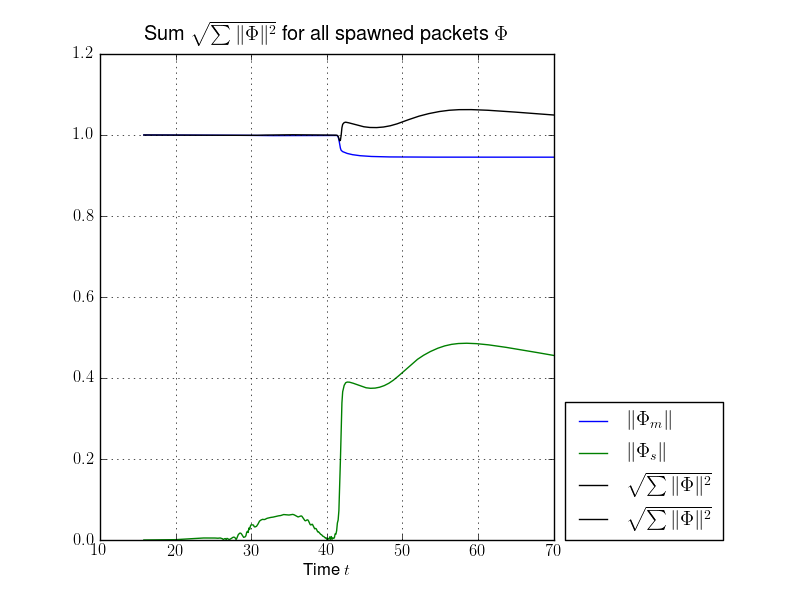
\includegraphics[width=0.5\linewidth]{./figures/norms_quad_mother.png}
  }
  \subfloat[][]{
    \label{fig:quad_drift_mother}
    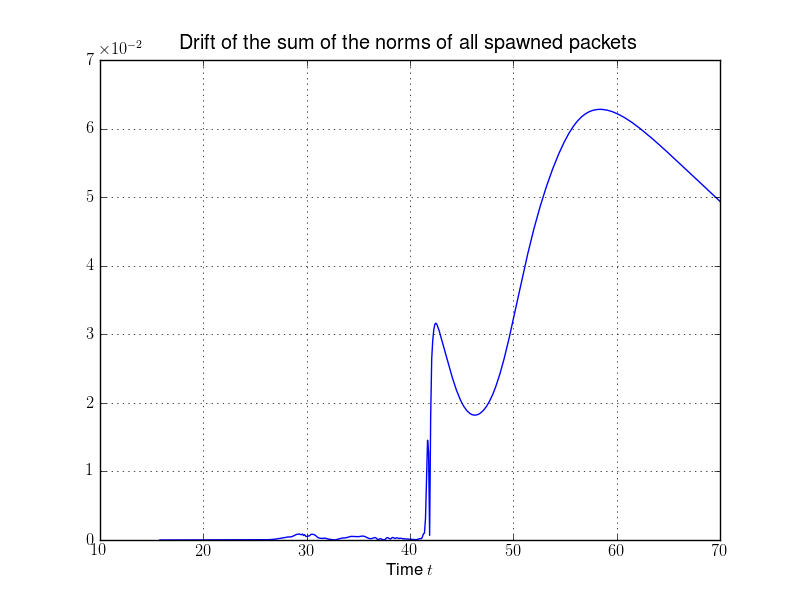
\includegraphics[width=0.5\linewidth]{./figures/norms_drift_quad_mother.png}
  } \\
  \subfloat[][]{
    \label{fig:quad_child}
    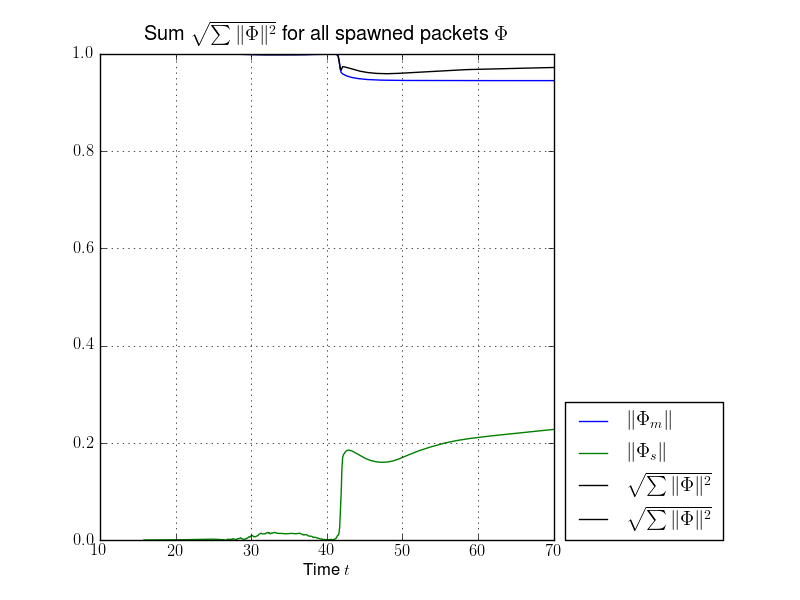
\includegraphics[width=0.5\linewidth]{./figures/norms_quad_child.png}
  }
  \subfloat[][]{
    \label{fig:quad_drift_child}
    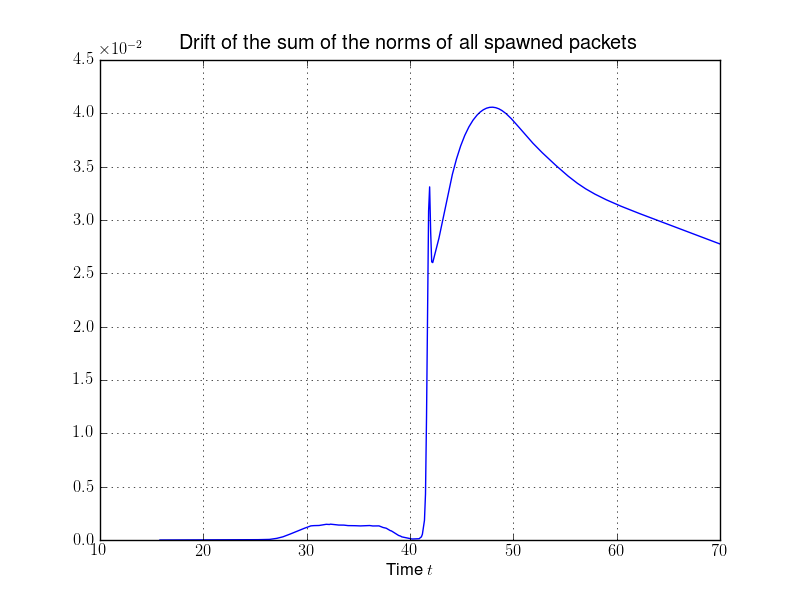
\includegraphics[width=0.5\linewidth]{./figures/norms_drift_quad_child.png}
  } \\
  \subfloat[][]{
    \label{fig:quad_mix}
    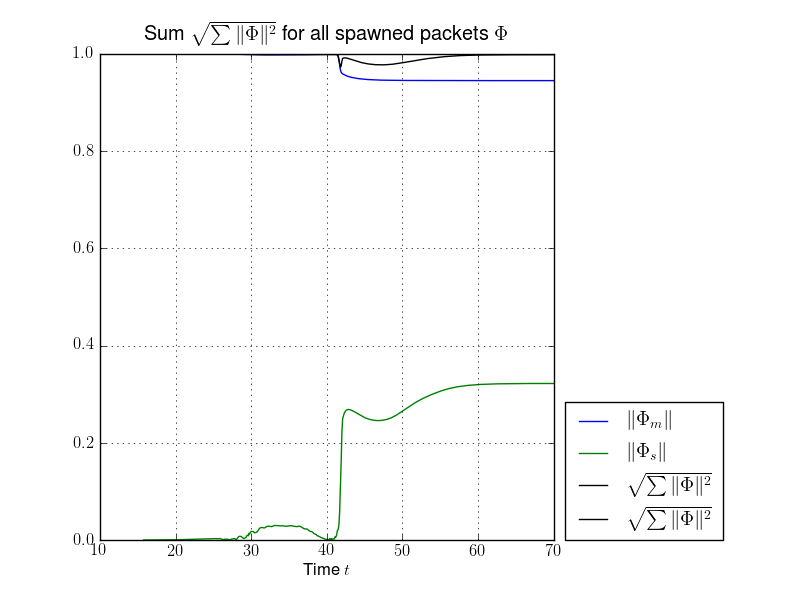
\includegraphics[width=0.5\linewidth]{./figures/norms_quad_mix.png}
  }
  \subfloat[][]{
    \label{fig:quad_drift_mix}
    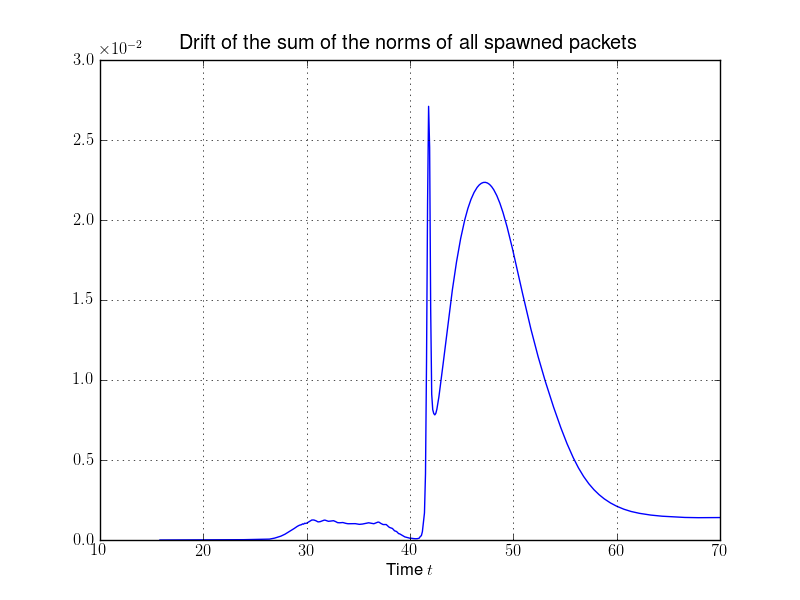
\includegraphics[width=0.5\linewidth]{./figures/norms_drift_quad_mix.png}
  } \\
  \caption[Comparison of quadratures used for basis projection]{
  The plots show the norms and the norm drift obtained by spawning with
  the projection method. For the quadrature used inside the projection method there
  are three possibilities: the quadrature can be homogeneous and focused on either
  the mother or the child (spawned) wavepacket. Or it can be the fully inhomogeneous
  quadrature, which is the only correct choice from the mathematical point of
  view and also yields the least and most rapidly decaying error.
  \subref{fig:quad_mother} Norm, computed with quadrature focused on the mother part.
  \subref{fig:quad_drift_mother} Difference to the theoretical norm, computed with quadrature focused on the mother part.
  \subref{fig:quad_child} Norm, computed with quadrature focused on the child part.
  \subref{fig:quad_drift_child} Difference to the theoretical norm, computed with quadrature focused on the child part.
  \subref{fig:quad_mix} Norm, computed with inhomogeneous quadrature.
  \subref{fig:quad_drift_mix} Difference to the theoretical norm, computed with inhomogeneous quadrature.
  \label{fig:quadrature_choice}
  }
\end{figure}

Algorithm \ref{al:projection_method} shows an algorithmic formulation of basis
projection method. The code is inefficient because of the nested loops and the
actual implementation uses several optimizations like vectorization and contains
no explicit loop.

\begin{algorithm}
\caption{Basis projection method for the change of basis}
\label{al:projection_method}
\begin{algorithmic}
  \REQUIRE The size $K$ of the old and $\eta$ of the new basis
  \REQUIRE The parameters $\Pi$ and $\tilde{\Pi}$ defining the bases
  \REQUIRE The two sets of basis functions $\{\phi_k\}_{k=0}^{K-1}$ and $\{\tilde{\phi}_k\}_{k=0}^{\eta-1}$
  \REQUIRE The mother fragment $w$ with its coefficients $\{c_k\}_{k=\alpha}^{\beta}$
  \REQUIRE A mixing quadrature rule of order $R$ with nodes $\gamma$ and weights $\omega$
  \REQUIRE A value for $\mu \in \{0, \ldots, \eta-1\}$
  \REQUIRE $\alpha \geq 0$ and $\beta \leq K-1$

  \STATE // Compute $Q_S$ from mixing $\Pi$ and $\tilde{\Pi}$ by the mixing procedure \ref{al:mixing_hagedorn_parameters}
  \STATE $Q_S \assign \text{mix\_parameters}(\Pi, \tilde{\Pi})$

  \STATE // Initialize all new coefficients with zero
  \STATE $\left(d_0, \ldots, d_{\eta-1}\right) \assign 0$

  \STATE // Project to the basis of the spawned part and compute new coefficients

  \FOR{$i \assign 0$ \TO $\mu$}
    \FOR{$r \assign 0$ \TO $R-1$}
      \STATE $d_i \assign d_i + \conj{  \sum_{k=\alpha}^\beta c_k \phi_k\ofs{\gamma_r}} \cdot \tilde{\phi}_i \ofs{\gamma_r} \cdot \omega_r$
    \ENDFOR
    \STATE $d_i \assign \varepsilon \cdot Q_S \cdot d_i$
  \ENDFOR

  \STATE // Set the old coefficients to zero
  \STATE $\left(c_\alpha, \ldots, c_\beta\right) \assign 0$

  \RETURN $d \assign \left(d_0, \ldots, d_{\eta-1}\right)$
\end{algorithmic}
\end{algorithm}


\section{Problematic difficulties and open issues}

Now we can return to the problem of choosing concrete values for $\tilde{P}$ and $\tilde{Q}$
we deferred at the end of section \ref{sec:pq}. After we developed the formalism
to really create the spawned fragments $\tilde{w}$ in the last section we can
now use this to determine the best choice among the four possibilities of \eqref{eq:pq_possibilities}.
The idea is to spawn a fragment using each of these four different parameter pairs
resulting in the test fragments $\tilde{w_1}, \tilde{w_2}, \tilde{w_3} \text{ and } \tilde{w_4}$.
And then we can try to maximize the overlap with the original fragment $w$

\begin{equation}
  \arg \max_i \Braket{\tilde{w_i}|w} \,.
\end{equation}

This gives us then the best pair of parameters and we can finish the set $\tilde{\Pi}$.
The drawback of this method is that while the original parameters $P\ofs{t}$ and
$Q\ofs{t}$ are continuous and smooth functions of time, this maximization procedure
can introduce arbitrary jumps. Hence while this method works most of the time
and these jumps do not matter for our purposes it's still not the optimal solution.
When we combine spawning and propagation later these jumps won't be a problem
because we spawn once and the propagate smoothly.

~\newline

Another severe problem already mentioned above is posed by the $k$ in formula
\eqref{eq:estimate_abssqrPQ}. In general we do not work with single basis functions
but with fragments which are linear combinations thereof. Therefore we need to
estimate the parameters for such a linear combination to get a good basis for spawning.
We have no way to know a value of $k$ at spawning time and we also have no suitable
way to compute it. For the tunneling problem it can be shown \cite{GHJ_exponentially_accurate}
that the transmitted part is always a Gaussian (at least asymptotically for large times)
and hence we can set $k=0$ there and spawn a $\phi_0$ by lumping. (The procedure
still works for the basis projection method, but depends on the fact that
we can set $k=0$ as justified by theory.) More on this in the next chapter.

In the non-adiabatic case $k$ can have any value. Additionally we won't spawn
just a single function $\phi_k$ but a whole linear combination $\sum_i \phi_i$.
Under these circumstances it is even more obscure what $k$ should be. A real world
example is shown in figure \ref{fig:spawn_issues_k_na} where we would like to
spawn on the lower level. The fragment there has clearly the shape of a $\phi_2$
but setting $k=2$ can not be justified if we look at the lower right panel.

\begin{figure}
  \centering
  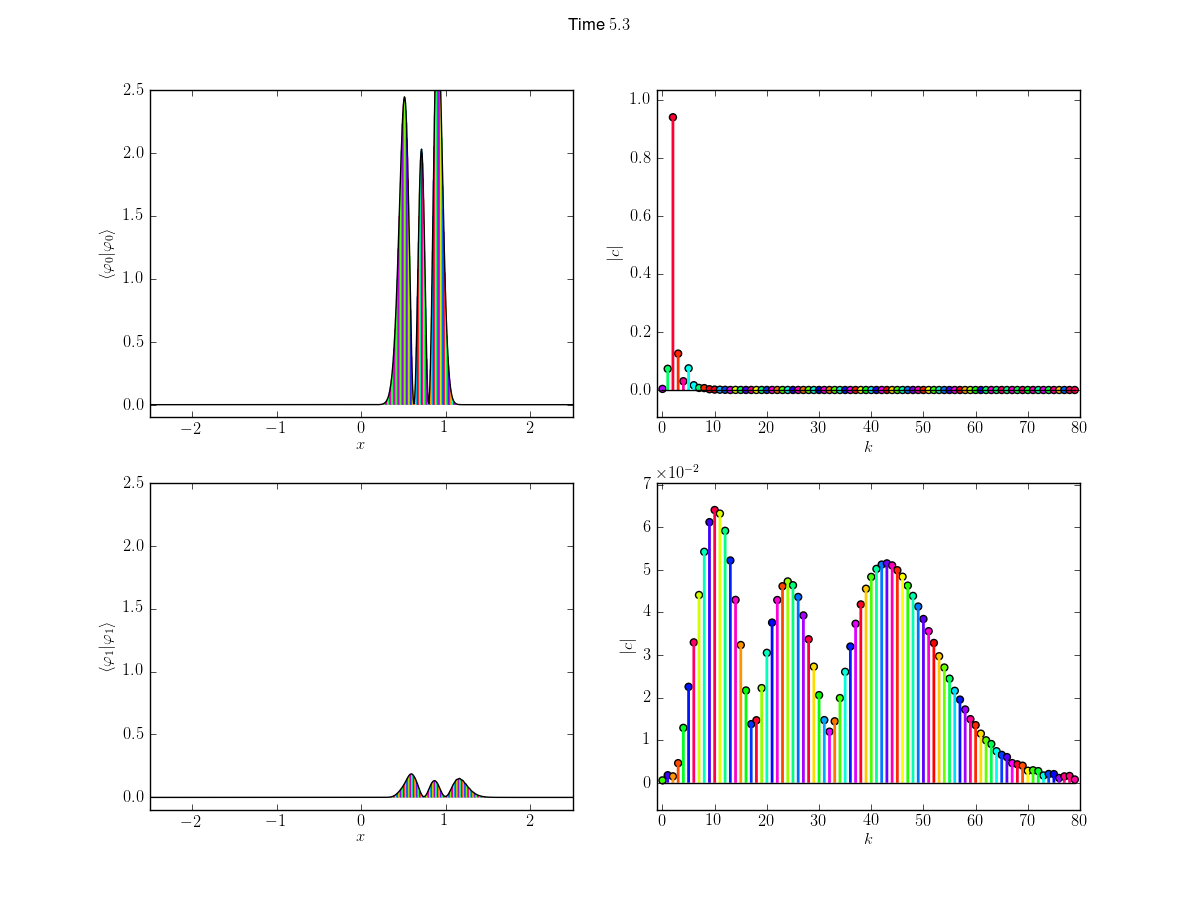
\includegraphics[width=\linewidth]{./figures/spawn_issues_k_na.png}
  \caption[Snapshot of a $\phi_2$ wavepacket in an avoided crossing]{If we spawn
  on the upper level then we can justify to choose $k=2$ but when we would like
  to spawn on the lower level, it is by far not obvious how to choose $k$. One
  could start guessing and try f.e. the median. In both cases the fragment (left
  panels) used for estimating parameters has the shape of a $\phi_2$.}
  \label{fig:spawn_issues_k_na}
\end{figure}

~\newline

The last open issue we would like to mention here is that sometimes the relation

\begin{equation}
  |\tilde{P}|^2 |\tilde{Q}|^2 \geq 1
\end{equation}

is violated. This is really bad because this inequality expresses Heisenberg's
uncertainty principle which is fundamental in quantum physics and should always
be fulfilled, see also \cite[remark 2.7]{H_ladder_operators}. Violations of this
inequality will in turn induce a violation of the compatibility relations \eqref{eq:symplecticity_condition}.

The origin of these problems is again formula \eqref{eq:estimate_abssqrPQ}. The
equation shown there is mathematically only correct for single basis functions
$\phi_k$ and does not provide any solution for linear combinations like our
fragments. Because of this it is strictly speaking not allowed to plug in
the estimated second moments of $w$ as we did. This discrepancy is what
causes the violation of the uncertainty principle. Luckily for us it happened
in the simulations only at times where spawning would make no sense anyway.
And we should add that it never happened if $k=0$ but this is no solution either
as it will hinder the spawning process taking place at times when the
violation is not present.

It's not clear what the best way to proceed from here is. Also it's not clear how
important an accurate guess of $\tilde{P}$ and $\tilde{Q}$ really is. For example
one can obtain a decent result by performing spawning by doing basis projection
and using a large enough target basis.

\end{chapter}


\clearemptydoublepage

\begin{chapter}{Spawning in tunneling problems}
\label{ch:spawntunneling}

In this chapter we will apply the theoretical ideas of spawning developed in the
last chapter to the tunneling problem which motivated these ideas in the first place.
We will briefly review the original work from the paper \cite{GHJ_tunneling_spawning}
and then extend these ideas further. We will explore the advantages of the new
projection method over the lumping method for spawning and see how this helps
to get better results at finite times. What was done in that paper is a procedure
we call now \emph{aposteriori spawning} because we need a full simulation before
we can start to analyze the benefits of spawning. While this provides us with
insight to the fundamental process, we need to interleave spawning and propagation
tightly if we want to improve the simulation algorithms in practice. If done
right this reduces the wall time and memory cost drastically. But it is a highly
non-trivial task with many pitfalls potentially turning the simulation results
into garbage. We will look at all these details in the section on
\emph{spawning and propagation}.


\section{Adapting the theoretical basis}

In a first step we adapt the theory from the last chapter to the tunneling
problem. This gives simplified formulae for computing the spawned wavepackets.
In the tunneling problem our original wavepacket $\Ket{\Psi}$ has only a single
component $\Phi_0$ and the potential consists of a single real valued function.
An example for a typical potential was given in figure \ref{fig:eckart_potential}.
The component $\Phi_0$ is given according to the definition from \eqref{fig:eckart_potential}
with a basis of size $K$. Adapting the notation from \cite{GHJ_tunneling_spawning}
we write

\begin{equation} \label{eq:decompose_psi_tunnel}
  \Ket{\Psi} = u\ofs{t} \rassign v\ofs{t} + w\ofs{t}
\end{equation}

where we decompose the wavepacket into two parts. These two parts will approximately
be the reflected and the transmitted part of the incoming wavefunction. The main
point of this whole chapter is to try to replace the transmitted part $w$ by a newly
spawned wavepacket $\tilde{w}$. This spawned wavepacket will be independent from
the original $v$ and both can be propagated independently\footnote{This is not the
complete truth. The parameter sets $\Pi$ and $\tilde{\Pi}$ can be propagated independently
of each other by the usual algorithms from \cite{FGL_semiclassical_dynamics}. But
of course the packets may still interact and thus the coefficients $c$ and $\tilde{c}$
can not be propagated separately. In the case of the tunneling problem this rapidly
becomes negligible because the two packets reside on different sides of the potential
hill. We will return on this issue in more detail later.}.
The $w\ofs{t}$ from above is our fragment and we rewrite the equation in more detail as

\begin{equation}
  \Ket{\Psi} = \sum_{k=0}^{K_0-1} c_k \phi_k + \underbrace{\sum_{k=K_0}^{K-1} c_k \phi_k}_{\rassign w}
\end{equation}

where we omitted the global phase which is present for both summands.
The first few coefficients $c_0, \ldots, c_{K_0-1}$ are usually not interesting for
spawning, they remain at the mother wavepacket and belong to the reflected part.
For a picture of the actual situation we refer to figure \ref{fig:tunneling_highfreq}
from the last chapter. The value denoted by $K_0$ is the cutoff where the fragment
starts and hence we set $\alpha = K_0$ and $\beta = K-1$. For the estimated position
and momentum we plug in these values in \eqref{eq:estimate_pos} and \eqref{eq:estimate_mom}
and get

\begin{align}
  \tilde{q} & \assign \frac{\Braket{w | x | w}}{\Braket{w|w}}
            = \frac{\sqrt{2 \varepsilon^2}}{\sum_{k=K_0}^{K-1} \conj{c_k} c_k} \Re \left(Q \sum_{k=K_0+1}^{K-1} \conj{c_k} c_{k-1} \sqrt{k} \right) + q
            \label{eq:estimate_pos_tunnel} \\
  \tilde{p} & \assign \frac{\Braket{w | y | w}}{\Braket{w|w}}
            = \frac{\sqrt{2 \varepsilon^2}}{\sum_{k=K_0}^{K-1} \conj{c_k} c_k} \Re \left(P \sum_{k=K_0+1}^{K-1} \conj{c_k} c_{k-1} \sqrt{k} \right) + p \,.
            \label{eq:estimate_mom_tunnel}
\end{align}

These two formulae are equivalent to formula 14 and 15 from \cite{GHJ_tunneling_spawning}.
Notice that our sums stop at $K-1$ inclusive because our basis is of overall size $K$.
For the second moments we apply the same simplifications to \eqref{eq:est_second_moment_pos_final}
and \eqref{eq:est_second_moment_mom_final} which then yields

\begin{align} \label{eq:est_second_moment_pos_tunnel}
  \frac{\Braket{w|\left(x-\tilde{q}\right)^2|w}}{\Braket{w|w}} & =
  \frac{
    \varepsilon^2 \Re \left( Q^2 \sum_{k=K_0}^{K-3} \conj{c_{k+2}} c_{k} \sqrt{k^2+3k+2} \right)
    + \frac{\varepsilon^2}{2} |Q|^2 \sum_{k=K_0}^{K-1} \conj{c_k} c_k \left(2k+1\right)
  }{\sum_{k=K_0}^{K-1} \conj{c_k} c_k}
  - \left(q - \tilde{q}\right)^2 \\
  \label{eq:est_second_moment_mom_tunnel}
  \frac{\Braket{w|\left(x-\tilde{p}\right)^2|w}}{\Braket{w|w}} & =
  \frac{
    \varepsilon^2 \Re \left( P^2 \sum_{k=K_0}^{K-3} \conj{c_{k+2}} c_{k} \sqrt{k^2+3k+2} \right)
    + \frac{\varepsilon^2}{2} |P|^2 \sum_{k=K_0}^{K-1} \conj{c_k} c_k \left(2k+1\right)
  }{\sum_{k=K_0}^{K-1} \conj{c_k} c_k}
  - \left(p - \tilde{p}\right)^2 \,.
\end{align}

Additionally we can set $k=0$ in \eqref{eq:estimate_abssqrPQ} in this special setup
and get

\begin{equation}
\label{eq:estimate_abssqrPQ_tunnel}
\begin{split}
  |P|^2 & = \frac{2}{\varepsilon^2} \Braket{\phi_k | \left(x-p\right)^2 | \phi_k} \\
  |Q|^2 & = \frac{2}{\varepsilon^2} \Braket{\phi_k | \left(x-q\right)^2 | \phi_k} \,.
\end{split}
\end{equation}

The foundation for this step are theoretical results \cite{GHJ_exponentially_accurate}
proving that in the tunneling problem the transmitted part $w$ is at least
asymptotically always a Gaussian in leading order. Hence we can concentrate on
$\phi_0$ while estimating parameters\footnote{We exploit this fact only for $\tilde{P}$
and $\tilde{Q}$ and only in the final step there because of the troubles shown at the
end of the last chapter. For the second moments we still use the whole $w$ and
not only $\phi_0$. The same holds for the estimated position and momentum as we
can obtain exact results using the complete $w$ easily.}.
Plugging in the results from \eqref{eq:est_second_moment_pos_tunnel} and
\eqref{eq:est_second_moment_mom_tunnel} here replacing the brakets we end up with
two relations for $|\tilde{Q}|^2$ and $|\tilde{P}|^2$ which are equivalent to the
ones for $|A|^2$ and $|B|^2$ in the aforementioned paper. This is all we had to do
and we are now ready to use the lumping or projection methods directly as defined
in the algorithms \ref{al:lumping_method} and \ref{al:projection_method} for
spawning wavepackets in tunneling problems. This also concludes our review of the
theory part of reference \cite{GHJ_tunneling_spawning}.


\section{Aposteriori spawning}

In this section we will explain the term \emph{aposteriori spawning} in details.
This name stems from the fact, that all computations are done after the simulation.
It means that first we need a full simulation of the packet $\Ket{\Psi}$ being
propagated through time. During this simulation nothing related to spawning
happens. But afterwards we perform spawning computations and see what would happen
if we used spawning to improve the simulation. The whole effort only helps to
enhance our understanding of spawning. It does not provide us with a better
or faster simulation or more exact results. This can only be the case if we
use spawning \emph{during} the simulation.

In an aposteriori spawning simulation we do compute a spawned wavepacket for
each timestep of the original simulation. After we spawned the new packet,
we measure energies and norms and test how much error we introduced while spawning
this new wavepacket. Algorithm \ref{al:aposteriori_spawning} gives a more schematic
overview on how aposteriori spawning works in general.

\begin{algorithm}
\caption{Aposteriori spawning method (in general)}
\label{al:aposteriori_spawning}
\begin{algorithmic}
  \REQUIRE A time series $t$ consisting of timesteps $\{\tau_0, \ldots, \tau_{\text{max}}\}$
  \REQUIRE The wavepackets $\Psi\ofs{t}$ with parameters $\Pi$ and coefficients $\{c^i_k\}_{k=0}^{K-1}$
  \REQUIRE The component $0 \leq \nu \leq N$ of $\Psi$ examined for spawning
  \REQUIRE Integers $\alpha \geq 0$ and $\beta \leq K-1$

  \FORALL{$\tau_i \in t$}
    \STATE // Construct the fragment as subset of $\Phi_\nu$
    \STATE $w \assign \sum_{k=\alpha}^{\beta} c_k^\nu \phi_k$

    \STATE // Estimate the parameters of the fragment by algorithm \ref{al:parameter_estimation}
    \STATE $\tilde{\Pi} \assign \textbf{estimate\_parameters}(w)$
    \STATE // Move the fragment $w$ to the new basis by either algorithm \ref{al:lumping_method} or \ref{al:projection_method}
    \STATE $\tilde{w} \assign \textbf{change\_basis}(\tilde{\Pi}, w)$
    \STATE // Measure norms, energies etc
    \STATE $\textbf{measure}(\tilde{w})$
  \ENDFOR
\end{algorithmic}
\end{algorithm}

For the tunneling problem this algorithm simplifies a little bit. First our
packet $\Ket{\Psi}$ consists only of a single component $\Phi_0$ and we set
$\nu = 0$. Then we are interested in removing the high frequencies from
the original wavepacket and put them into a new packet where the same information
on the wavefunction can be (approximately) represented by much less and lower frequencies.
Hence we set $\beta = K-1$ and $\alpha = K_0$ where the correct choice of $K_0$ poses
a new problem. Luckily it turns out that this choice is not critical as long
as there is a region around $K_0$ where the coefficients $c_i$ are very small.
In other words, there are two bulges of large coefficients separated by a region
with almost zeros and we can choose $K_0$ arbitrary but well within this region.
If we refer to figure \ref{fig:tunneling_highfreq} then this region would range
from about $40$ up to about $100$ and we can choose $K_0 = 50$. But we should keep
in mind that for more advanced applications of spawning it may be difficult or
even impossible to know a good $K_0$ a priori. In the aposteriori spawning process
this has no importance as we can always look at the coefficients of the original
simulation. For the spawning propagation algorithm one could try to use some
statistical methods developed for classification problems.


\FloatBarrier
\section{Basic tunneling simulations}

In this section we show the results of three tunneling simulations.
First we send a wavepacket $\Ket{\Psi} = \phi_0$ from the left. Then we try the
same simulation setup with a $\phi_2$ and a $\phi_3$. All three simulations
are very similar in the sense that we use the same initial parameters for
the wavepackets with the only exception being the reduced momentum for the later
two. The following plots build the reference to which we compare the various
spawning approaches from the next section.

\begin{figure}[h!]
  \centering
  \subfloat[][]{
    \label{fig:traject_phi0_P}
    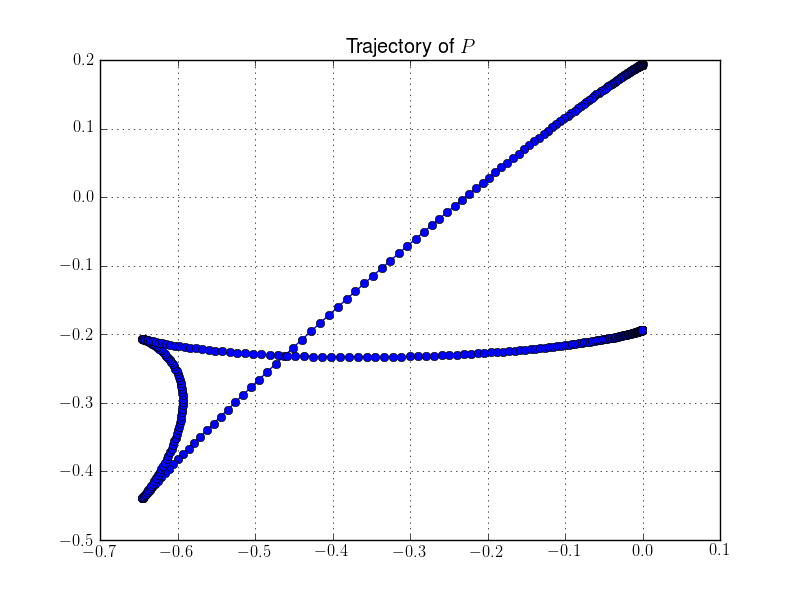
\includegraphics[width=0.5\linewidth]{./figures/tunnel_basic/phi0_trajectory_P.png}
  }
  \subfloat[][]{
    \label{fig:traject_phi0_Q}
    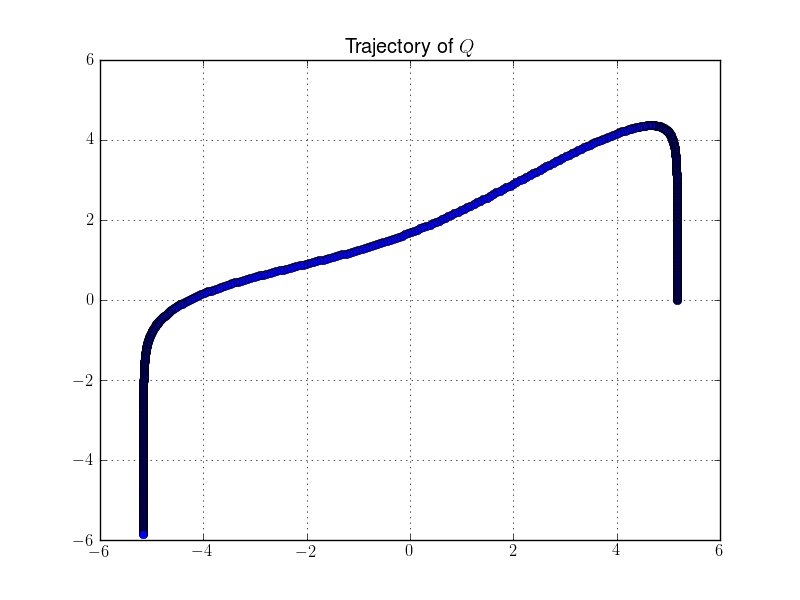
\includegraphics[width=0.5\linewidth]{./figures/tunnel_basic/phi0_trajectory_Q.png}
  } \\
  \caption[Complex trajectories for $P$ and $Q$]{
  The plot shows the trajectories of the parameters $P$ and $Q$ in the complex plane.
  The simulation parameters are shown in \ref{cfg:tunneling_phi0}.
  \label{fig:traject_phi0}
  }
\end{figure}

\begin{figure}[h!]
  \centering
  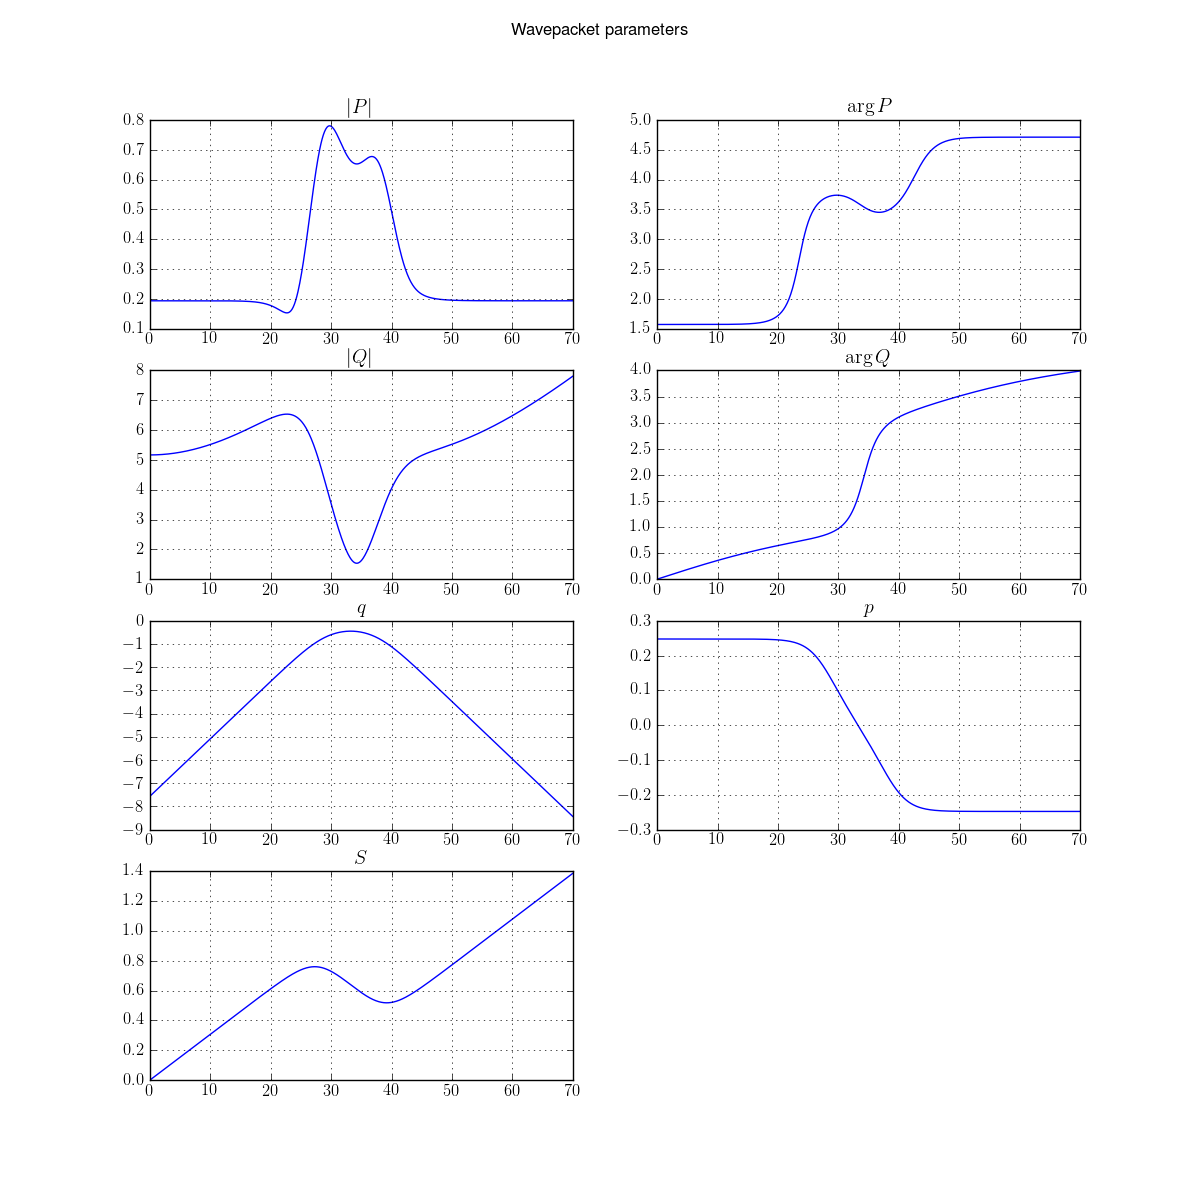
\includegraphics[width=\the\linewidth]{./figures/tunnel_basic/parameters_phi0.png}
  \caption[The parameter set $\Pi$ of the simulation with $\phi_0$]
  {The parameter set $\Pi$ of the simulation with $\phi_0$ plotted versus time.
  The simulation parameters are shown in \ref{cfg:tunneling_phi0}.}
\end{figure}

\begin{figure}[h!]
  \centering
  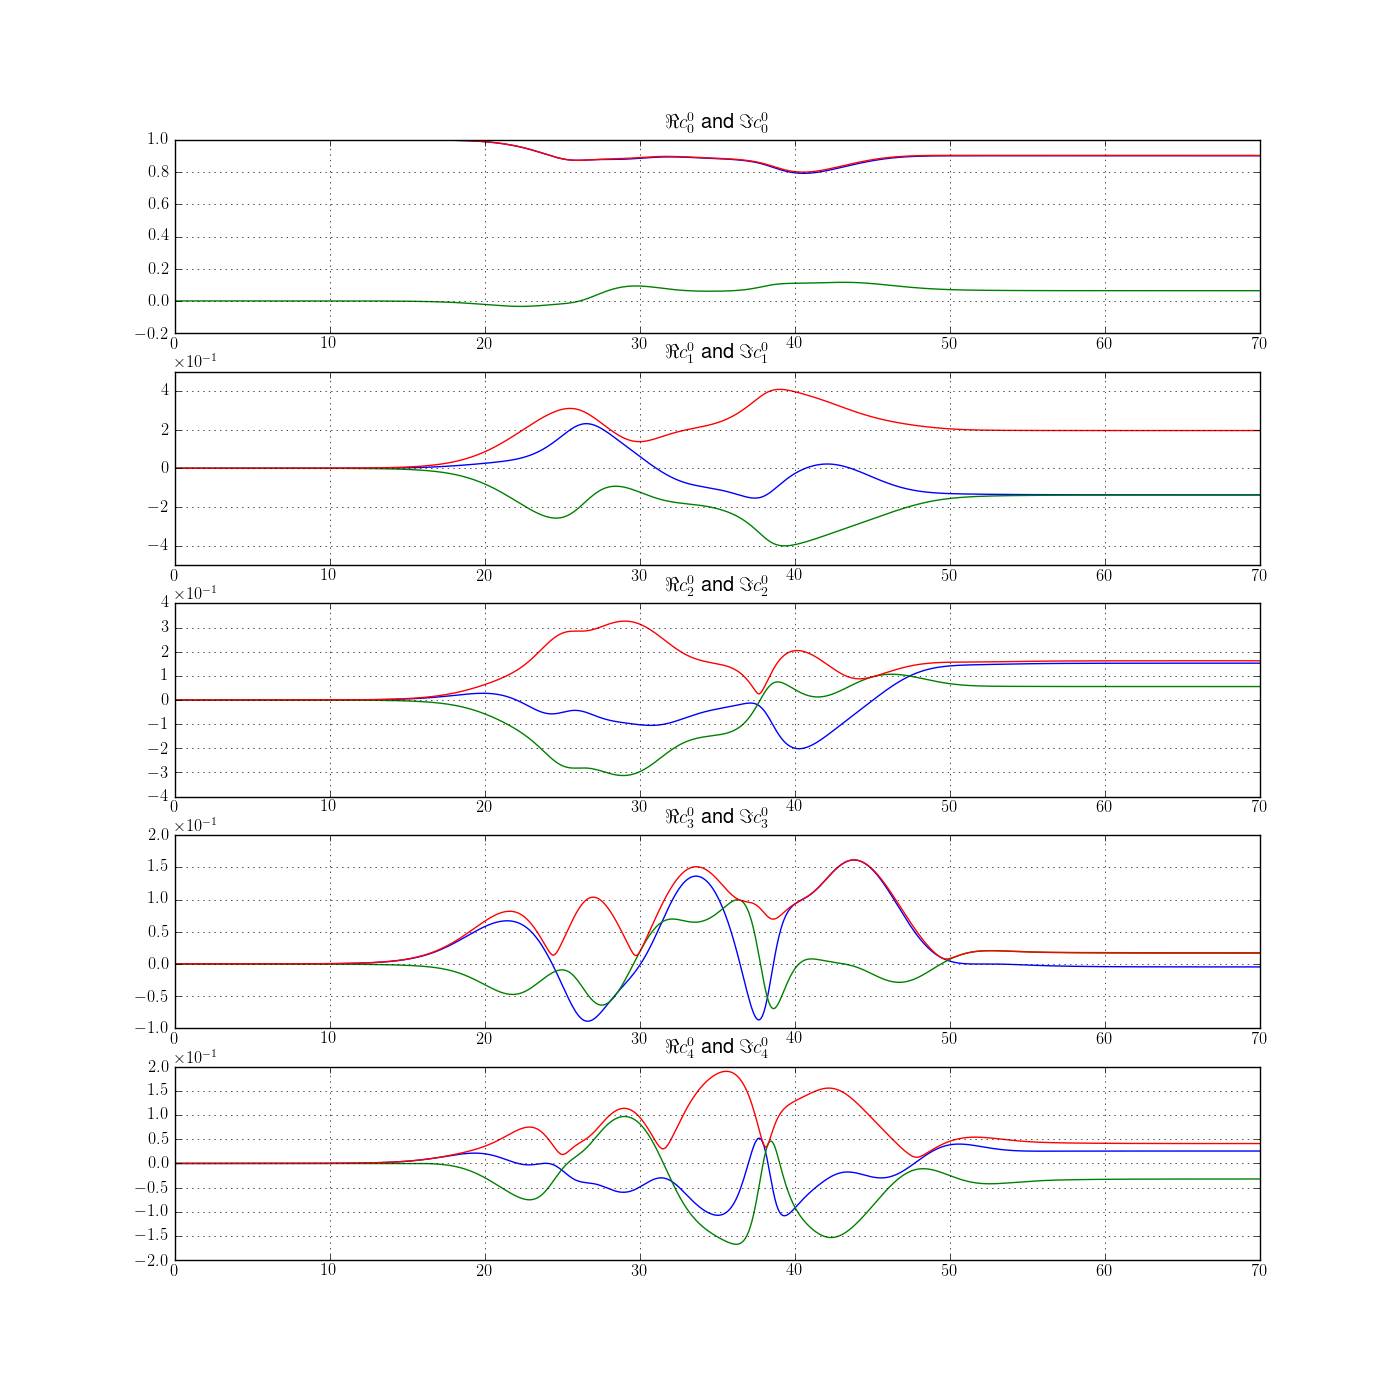
\includegraphics[width=\the\linewidth]{./figures/tunnel_basic/coefficients_first_phi0.png}
  \caption[The first few coefficients $c_i$ of the simulation with $\phi_0$]
  {The first few coefficients $c_i$ of the simulation with $\phi_0$ plotted versus time.
  The simulation parameters are shown in \ref{cfg:tunneling_phi0}.}
\end{figure}

\begin{figure}
  \centering
  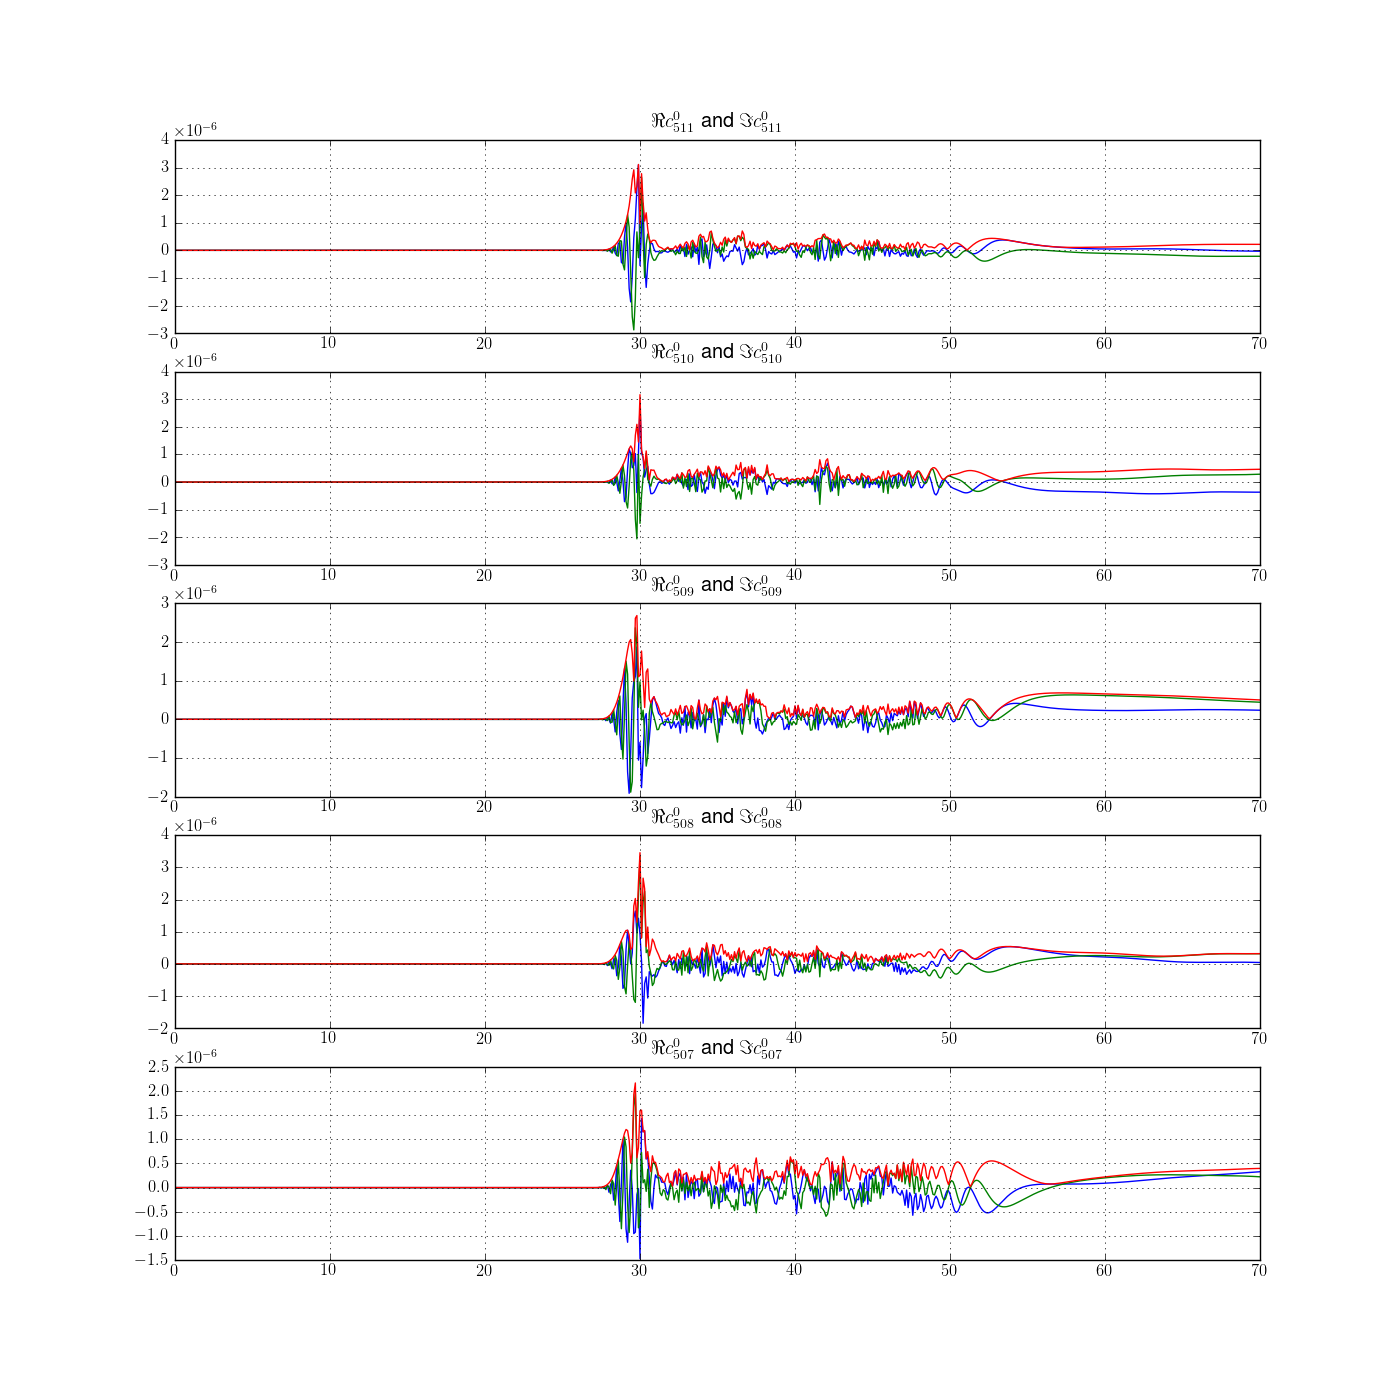
\includegraphics[width=\the\linewidth]{./figures/tunnel_basic/coefficients_last_phi0.png}
  \caption[The last few coefficients $c_i$ of the simulation with $\phi_0$]
  {The last few coefficients $c_i$ of the simulation with $\phi_0$ plotted versus time.
  We see that their values are really small and thus the loss due to the finite basis is minimal.
  The simulation parameters are shown in \ref{cfg:tunneling_phi0}.}
\end{figure}

\begin{figure}[h!]
  \centering
  \subfloat[][]{
    \label{fig:tunnel_energy_phi0}
    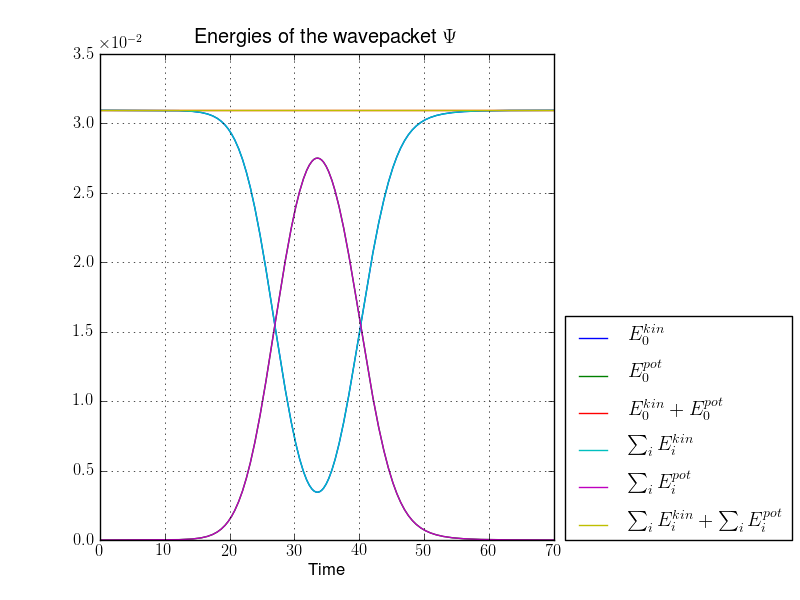
\includegraphics[width=0.5\linewidth]{./figures/tunnel_basic/energies_phi0.png}
  }
  \subfloat[][]{
    \label{fig:tunnel_energy_drift_phi0}
    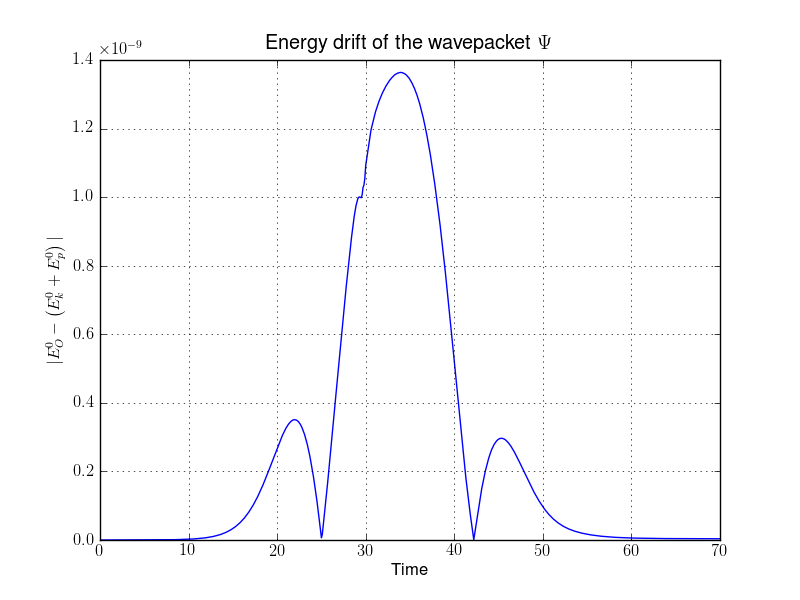
\includegraphics[width=0.5\linewidth]{./figures/tunnel_basic/energy_drift_phi0.png}
  } \\
  \subfloat[][]{
    \label{fig:tunnel_energy_phi2}
    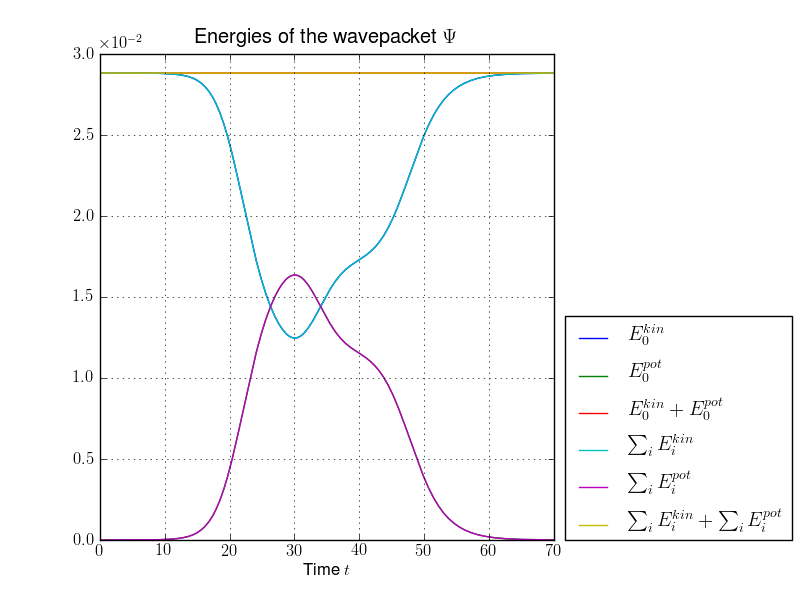
\includegraphics[width=0.5\linewidth]{./figures/tunnel_basic/energies_phi2.png}
  }
  \subfloat[][]{
    \label{fig:tunnel_energy_drift_phi2}
    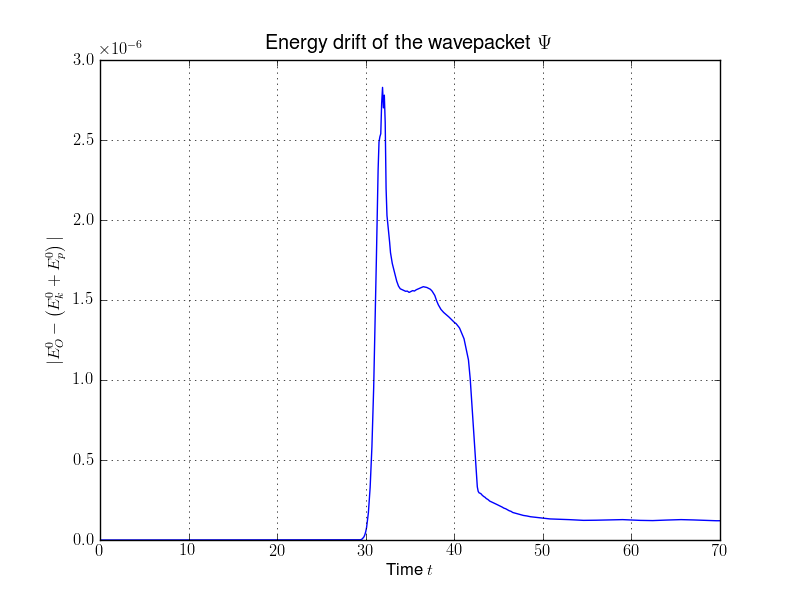
\includegraphics[width=0.5\linewidth]{./figures/tunnel_basic/energy_drift_phi2.png}
  } \\
  \subfloat[][]{
    \label{fig:tunnel_energy_phi3}
    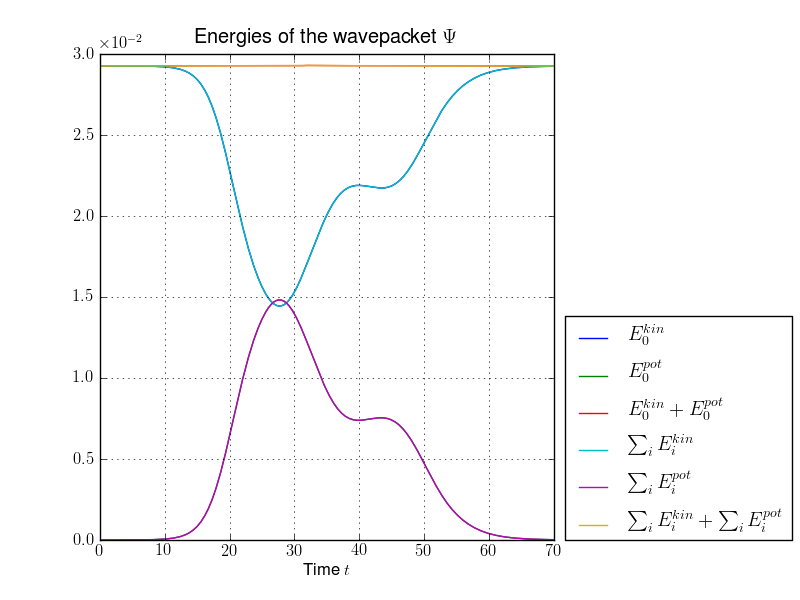
\includegraphics[width=0.5\linewidth]{./figures/tunnel_basic/energies_phi3.png}
  }
  \subfloat[][]{
    \label{fig:tunnel_energy_drift_phi3}
    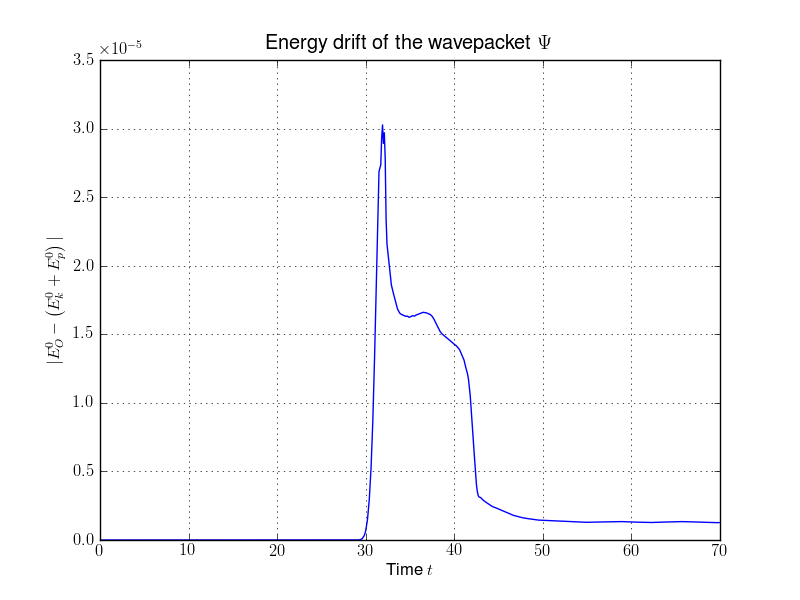
\includegraphics[width=0.5\linewidth]{./figures/tunnel_basic/energy_drift_phi3.png}
  } \\
  \caption[Energies and energy drift for some tunneling wavepackets]{
  This figure shows the energies and energy drift of several tunneling simulations.
  The simulation parameters are printed in \ref{cfg:tunneling_phi0}, \ref{cfg:tunneling_phi2} and \ref{cfg:tunneling_phi3}.
  \subref{fig:tunnel_energy_phi0} Kinetic and potential energy for a wavepacket $\phi_0$ tunneling through the Eckart barrier.
  \subref{fig:tunnel_energy_drift_phi0} Energy drift for a wavepacket $\phi_0$ tunneling through the Eckart barrier.
  \subref{fig:tunnel_energy_phi2} Kinetic and potential energy for a wavepacket $\phi_2$ tunneling through the Eckart barrier.
  \subref{fig:tunnel_energy_drift_phi2} Energy drift for a wavepacket $\phi_2$ tunneling through the Eckart barrier.
  \subref{fig:tunnel_energy_phi3} Kinetic and potential energy for a wavepacket $\phi_3$ tunneling through the Eckart barrier.
  \subref{fig:tunnel_energy_drift_phi3} Energy drift for a wavepacket $\phi_3$ tunneling through the Eckart barrier.
  \label{fig:tunnel_energies}
  }
\end{figure}

\begin{figure}[h!]
  \centering
  \subfloat[][]{
    \label{fig:tunnel_norm_drift_phi0}
    \includegraphics[width=0.5\linewidth]{./figures/tunnel_basic/norms_drift_phi0.png}
  }
  \subfloat[][]{
    \label{fig:tunnel_norm_drift_phi2}
    \includegraphics[width=0.5\linewidth]{./figures/tunnel_basic/norms_drift_phi2.png}
  } \\
  \subfloat[][]{
    \label{fig:tunnel_norm_drift_phi3}
    \includegraphics[width=0.5\linewidth]{./figures/tunnel_basic/norms_drift_phi3.png}
  }
  \caption[Norm drift for some tunneling wavepackets]{
  This figure shows the drift of the norm for several tunneling simulations. We have very good
  norm conservation. The reason for this is that we used a huge basis with $K=512$.
  The simulation parameters are printed in \ref{cfg:tunneling_phi0}, \ref{cfg:tunneling_phi2} and \ref{cfg:tunneling_phi3}.
  \subref{fig:tunnel_norm_drift_phi0} Norm drift for a wavepacket $\phi_0$ tunneling through the Eckart barrier.
  \subref{fig:tunnel_norm_drift_phi2} Norm drift for a wavepacket $\phi_2$ tunneling through the Eckart barrier.
  \subref{fig:tunnel_norm_drift_phi3} Norm drift for a wavepacket $\phi_3$ tunneling through the Eckart barrier.
  \label{fig:tunnel_norms}
  }
\end{figure}


\FloatBarrier
\section{Spawning using the lumping method}

Now we try aposteriori spawning based on the simulation from the last section.
In the first examples we use the lumping method which works quite well for large
enough times. The spawned packet has the shape of a Gaussian and we set $k=0$ for
lumping. The initial values of $\Ket{\Psi}$ are taken to be $\phi_0$, $\phi_2$
and $\phi_3$. We try different values for the parameter $K_0$ and compare the
estimated parameter sets $\tilde{\Pi}$.


\begin{figure}[h!]
  \centering
  \subfloat[][]{
    \label{fig:spawn_eckart_apost_phi0_K050_norms}
    \includegraphics[width=0.5\linewidth]{./figures/eckart_spawn_apost_phi0_K50/norms_compare_sumall_group0.pdf}
  }
  \subfloat[][]{
    \label{fig:spawn_eckart_apost_phi0_K050_norms_drift}
    \includegraphics[width=0.5\linewidth]{./figures/eckart_spawn_apost_phi0_K50/norms_compare_components_diff_group0.pdf}
  } \\
  \subfloat[][]{
    \label{fig:spawn_eckart_apost_phi0_K075_norms}
    \includegraphics[width=0.5\linewidth]{./figures/eckart_spawn_apost_phi0_K75/norms_compare_sumall_group0.pdf}
  }
  \subfloat[][]{
    \label{fig:spawn_eckart_apost_phi0_K075_norms_drift}
    \includegraphics[width=0.5\linewidth]{./figures/eckart_spawn_apost_phi0_K75/norms_compare_components_diff_group0.pdf}
  } \\
  \subfloat[][]{
    \label{fig:spawn_eckart_apost_phi0_K0100_norms}
    \includegraphics[width=0.5\linewidth]{./figures/eckart_spawn_apost_phi0_K100/norms_compare_sumall_group0.pdf}
  }
  \subfloat[][]{
    \label{fig:spawn_eckart_apost_phi0_K0100_norms_drift}
    \includegraphics[width=0.5\linewidth]{./figures/eckart_spawn_apost_phi0_K100/norms_compare_components_diff_group0.pdf}
  } \\
  \caption[Norms and norm drift for an aposteriori spawning simulation with lumping]{
  Norms and norm drift for an aposteriori spawning simulation based on the tunneling
  simulation of $\phi_0$. We see perfect norm conservation which has to be expected
  because of the lumping process which is lossless.
  \subref{fig:spawn_eckart_apost_phi0_K050_norms} $\Psi = \phi_0$ and $K_0=50$
  \subref{fig:spawn_eckart_apost_phi0_K050_norms_drift} $\Psi = \phi_0$ and $K_0=50$
  \subref{fig:spawn_eckart_apost_phi0_K075_norms} $\Psi = \phi_0$ and $K_0=75$
  \subref{fig:spawn_eckart_apost_phi0_K075_norms_drift} $\Psi = \phi_0$ and $K_0=75$
  \subref{fig:spawn_eckart_apost_phi0_K0100_norms} $\Psi = \phi_0$ and $K_0=100$
  \subref{fig:spawn_eckart_apost_phi0_K0100_norms_drift} $\Psi = \phi_0$ and $K_0=100$
  \label{fig:spawn_eckart_apost_phi0_norms}
  }
\end{figure}


\begin{figure}[h!]
  \centering
  \subfloat[][]{
    \label{fig:spawn_eckart_apost_phi2_K050_norms}
    \includegraphics[width=0.5\linewidth]{./figures/eckart_spawn_apost_phi2_K50/norms_compare_sumall_group0.pdf}
  }
  \subfloat[][]{
    \label{fig:spawn_eckart_apost_phi2_K050_norms_drift}
    \includegraphics[width=0.5\linewidth]{./figures/eckart_spawn_apost_phi2_K50/norms_compare_components_diff_group0.pdf}
  } \\
  \subfloat[][]{
    \label{fig:spawn_eckart_apost_phi2_K075_norms}
    \includegraphics[width=0.5\linewidth]{./figures/eckart_spawn_apost_phi2_K75/norms_compare_sumall_group0.pdf}
  }
  \subfloat[][]{
    \label{fig:spawn_eckart_apost_phi2_K075_norms_drift}
    \includegraphics[width=0.5\linewidth]{./figures/eckart_spawn_apost_phi2_K75/norms_compare_components_diff_group0.pdf}
  } \\
  \subfloat[][]{
    \label{fig:spawn_eckart_apost_phi2_K0100_norms}
    \includegraphics[width=0.5\linewidth]{./figures/eckart_spawn_apost_phi2_K100/norms_compare_sumall_group0.pdf}
  }
  \subfloat[][]{
    \label{fig:spawn_eckart_apost_phi2_K0100_norms_drift}
    \includegraphics[width=0.5\linewidth]{./figures/eckart_spawn_apost_phi2_K100/norms_compare_components_diff_group0.pdf}
  } \\
  \caption[Norms and norm drift for an aposteriori spawning simulation with lumping]{
  Norms and norm drift for an aposteriori spawning simulation based on the tunneling
  simulation of $\phi_2$. We see perfect norm conservation which has to be expected
  because of the lumping process which is lossless.
  \subref{fig:spawn_eckart_apost_phi2_K050_norms} $\Psi = \phi_2$ and $K_0=50$
  \subref{fig:spawn_eckart_apost_phi2_K050_norms_drift} $\Psi = \phi_2$ and $K_0=50$
  \subref{fig:spawn_eckart_apost_phi2_K075_norms} $\Psi = \phi_2$ and $K_0=75$
  \subref{fig:spawn_eckart_apost_phi2_K075_norms_drift} $\Psi = \phi_2$ and $K_0=75$
  \subref{fig:spawn_eckart_apost_phi2_K0100_norms} $\Psi = \phi_2$ and $K_0=100$
  \subref{fig:spawn_eckart_apost_phi2_K0100_norms_drift} $\Psi = \phi_2$ and $K_0=100$
  \label{fig:spawn_eckart_apost_phi2_norms}
  }
\end{figure}


\begin{figure}[h!]
  \centering
  \subfloat[][]{
    \label{fig:spawn_eckart_apost_phi3_K050_norms}
    \includegraphics[width=0.5\linewidth]{./figures/eckart_spawn_apost_phi3_K50/norms_compare_sumall_group0.pdf}
  }
  \subfloat[][]{
    \label{fig:spawn_eckart_apost_phi3_K050_norms_drift}
    \includegraphics[width=0.5\linewidth]{./figures/eckart_spawn_apost_phi3_K50/norms_compare_components_diff_group0.pdf}
  } \\
  \subfloat[][]{
    \label{fig:spawn_eckart_apost_phi3_K075_norms}
    \includegraphics[width=0.5\linewidth]{./figures/eckart_spawn_apost_phi3_K75/norms_compare_sumall_group0.pdf}
  }
  \subfloat[][]{
    \label{fig:spawn_eckart_apost_phi3_K075_norms_drift}
    \includegraphics[width=0.5\linewidth]{./figures/eckart_spawn_apost_phi3_K75/norms_compare_components_diff_group0.pdf}
  } \\
  \subfloat[][]{
    \label{fig:spawn_eckart_apost_phi3_K0100_norms}
    \includegraphics[width=0.5\linewidth]{./figures/eckart_spawn_apost_phi3_K100/norms_compare_sumall_group0.pdf}
  }
  \subfloat[][]{
    \label{fig:spawn_eckart_apost_phi3_K0100_norms_drift}
    \includegraphics[width=0.5\linewidth]{./figures/eckart_spawn_apost_phi3_K100/norms_compare_components_diff_group0.pdf}
  } \\
  \caption[Norms and norm drift for an aposteriori spawning simulation with lumping]{
  Norms and norm drift for an aposteriori spawning simulation based on the tunneling
  simulation of $\phi_3$. We see perfect norm conservation which has to be expected
  because of the lumping process which is lossless.
  \subref{fig:spawn_eckart_apost_phi3_K050_norms} $\Psi = \phi_3$ and $K_0=50$
  \subref{fig:spawn_eckart_apost_phi3_K050_norms_drift} $\Psi = \phi_3$ and $K_0=50$
  \subref{fig:spawn_eckart_apost_phi3_K075_norms} $\Psi = \phi_3$ and $K_0=75$
  \subref{fig:spawn_eckart_apost_phi3_K075_norms_drift} $\Psi = \phi_3$ and $K_0=75$
  \subref{fig:spawn_eckart_apost_phi3_K0100_norms} $\Psi = \phi_3$ and $K_0=100$
  \subref{fig:spawn_eckart_apost_phi3_K0100_norms_drift} $\Psi = \phi_3$ and $K_0=100$
  \label{fig:spawn_eckart_apost_phi3_norms}
  }
\end{figure}


\begin{figure}[h!]
  \centering
  \subfloat[][]{
    \label{fig:spawn_eckart_apost_phi0_K050_energies_components}
    \includegraphics[width=0.5\linewidth]{./figures/eckart_spawn_apost_phi0_K50/energies_compare_packetsum_group0.pdf}
  }
  \subfloat[][]{
    \label{fig:spawn_eckart_apost_phi0_K075_energies_components}
    \includegraphics[width=0.5\linewidth]{./figures/eckart_spawn_apost_phi0_K75/energies_compare_packetsum_group0.pdf}
  } \\
  \subfloat[][]{
    \label{fig:spawn_eckart_apost_phi0_K050_energies_sum}
    \includegraphics[width=0.5\linewidth]{./figures/eckart_spawn_apost_phi0_K50/energies_compare_components_group0.pdf}
  }
  \subfloat[][]{
    \label{fig:spawn_eckart_apost_phi0_K075_energies_sum}
    \includegraphics[width=0.5\linewidth]{./figures/eckart_spawn_apost_phi0_K75/energies_compare_components_group0.pdf}
  } \\
  \subfloat[][]{
    \label{fig:spawn_eckart_apost_phi0_K050_energies_drift}
    \includegraphics[width=0.5\linewidth]{./figures/eckart_spawn_apost_phi0_K50/energies_compare_components_diff_group0.pdf}
  }
  \subfloat[][]{
    \label{fig:spawn_eckart_apost_phi0_K075_energies_drift}
    \includegraphics[width=0.5\linewidth]{./figures/eckart_spawn_apost_phi0_K75/energies_compare_components_diff_group0.pdf}
  } \\
  \caption[Energies and energy drift for an aposteriori spawning simulation with lumping]{
  Energies and energy drift for an aposteriori spawning simulation. We try different initial
  for $\Ket{\Psi}$ and several values for $K_0$. Energy conservation for $\Psi = \phi_0$
  is by far good enough but not perfect.
  \subref{fig:spawn_eckart_apost_phi0_K050_energies_components} $\Psi = \phi_0$ and $K_0=50$
  \subref{fig:spawn_eckart_apost_phi0_K075_energies_components} $\Psi = \phi_0$ and $K_0=75$
  \subref{fig:spawn_eckart_apost_phi0_K050_energies_sum} $\Psi = \phi_0$ and $K_0=50$
  \subref{fig:spawn_eckart_apost_phi0_K075_energies_sum} $\Psi = \phi_0$ and $K_0=75$
  \subref{fig:spawn_eckart_apost_phi0_K050_energies_drift} $\Psi = \phi_0$ and $K_0=50$
  \subref{fig:spawn_eckart_apost_phi0_K075_energies_drift} $\Psi = \phi_0$ and $K_0=75$
  \label{fig:spawn_eckart_apost_lump_energies1}
  }
\end{figure}


\begin{figure}[h!]
  \centering
  \subfloat[][]{
    \label{fig:spawn_eckart_apost_phi0_K0100_energies_components}
    \includegraphics[width=0.5\linewidth]{./figures/eckart_spawn_apost_phi0_K100/energies_compare_packetsum_group0.pdf}
  }
  \subfloat[][]{
    \label{fig:spawn_eckart_apost_phi2_K050_energies_components}
    \includegraphics[width=0.5\linewidth]{./figures/eckart_spawn_apost_phi2_K50/energies_compare_packetsum_group0.pdf}
  } \\
  \subfloat[][]{
    \label{fig:spawn_eckart_apost_phi0_K0100_energies_sum}
    \includegraphics[width=0.5\linewidth]{./figures/eckart_spawn_apost_phi0_K100/energies_compare_components_group0.pdf}
  }
  \subfloat[][]{
    \label{fig:spawn_eckart_apost_phi2_K050_energies_sum}
    \includegraphics[width=0.5\linewidth]{./figures/eckart_spawn_apost_phi2_K50/energies_compare_components_group0.pdf}
  } \\
  \subfloat[][]{
    \label{fig:spawn_eckart_apost_phi0_K0100_energies_drift}
    \includegraphics[width=0.5\linewidth]{./figures/eckart_spawn_apost_phi0_K100/energies_compare_components_diff_group0.pdf}
  }
  \subfloat[][]{
    \label{fig:spawn_eckart_apost_phi2_K050_energies_drift}
    \includegraphics[width=0.5\linewidth]{./figures/eckart_spawn_apost_phi2_K50/energies_compare_components_diff_group0.pdf}
  } \\
  \caption[Energies and energy drift for an aposteriori spawning simulation with lumping]{
  Energies and energy drift for an aposteriori spawning simulation. We try different initial
  for $\Ket{\Psi}$ and several values for $K_0$. Energy conservation for $\Psi = \phi_0$
  is by far good enough but not perfect.
  \subref{fig:spawn_eckart_apost_phi0_K0100_energies_components} $\Psi = \phi_0$ and $K_0=100$
  \subref{fig:spawn_eckart_apost_phi2_K050_energies_components} $\Psi = \phi_2$ and $K_0=50$
  \subref{fig:spawn_eckart_apost_phi0_K0100_energies_sum} $\Psi = \phi_0$ and $K_0=100$
  \subref{fig:spawn_eckart_apost_phi2_K050_energies_sum} $\Psi = \phi_2$ and $K_0=50$
  \subref{fig:spawn_eckart_apost_phi0_K0100_energies_drift} $\Psi = \phi_0$ and $K_0=100$
  \subref{fig:spawn_eckart_apost_phi2_K050_energies_drift} $\Psi = \phi_2$ and $K_0=50$
  \label{fig:spawn_eckart_apost_lump_energies2}
  }
\end{figure}


\begin{figure}[h!]
  \centering
  \subfloat[][]{
    \label{fig:spawn_eckart_apost_phi2_K075_energies_components}
    \includegraphics[width=0.5\linewidth]{./figures/eckart_spawn_apost_phi2_K75/energies_compare_packetsum_group0.pdf}
  }
  \subfloat[][]{
    \label{fig:spawn_eckart_apost_phi2_K0100_energies_components}
    \includegraphics[width=0.5\linewidth]{./figures/eckart_spawn_apost_phi2_K100/energies_compare_packetsum_group0.pdf}
  } \\
  \subfloat[][]{
    \label{fig:spawn_eckart_apost_phi2_K075_energies_sum}
    \includegraphics[width=0.5\linewidth]{./figures/eckart_spawn_apost_phi2_K75/energies_compare_components_group0.pdf}
  }
  \subfloat[][]{
    \label{fig:spawn_eckart_apost_phi2_K0100_energies_sum}
    \includegraphics[width=0.5\linewidth]{./figures/eckart_spawn_apost_phi2_K100/energies_compare_components_group0.pdf}
  } \\
  \subfloat[][]{
    \label{fig:spawn_eckart_apost_phi2_K075_energies_drift}
    \includegraphics[width=0.5\linewidth]{./figures/eckart_spawn_apost_phi2_K75/energies_compare_components_diff_group0.pdf}
  }
  \subfloat[][]{
    \label{fig:spawn_eckart_apost_phi2_K0100_energies_drift}
    \includegraphics[width=0.5\linewidth]{./figures/eckart_spawn_apost_phi2_K100/energies_compare_components_diff_group0.pdf}
  } \\
  \caption[Energies and energy drift for an aposteriori spawning simulation with lumping]{
  Energies and energy drift for an aposteriori spawning simulation. We try different initial
  for $\Ket{\Psi}$ and several values for $K_0$. Energy conservation is only fulfilled after
  the tunneling event happened and tends to get better with higher $K_0$.
  \subref{fig:spawn_eckart_apost_phi2_K075_energies_components} $\Psi = \phi_2$ and $K_0=75$
  \subref{fig:spawn_eckart_apost_phi2_K0100_energies_components} $\Psi = \phi_2$ and $K_0=100$
  \subref{fig:spawn_eckart_apost_phi2_K075_energies_sum} $\Psi = \phi_2$ and $K_0=75$
  \subref{fig:spawn_eckart_apost_phi2_K0100_energies_sum} $\Psi = \phi_2$ and $K_0=100$
  \subref{fig:spawn_eckart_apost_phi2_K075_energies_drift} $\Psi = \phi_2$ and $K_0=75$
  \subref{fig:spawn_eckart_apost_phi2_K0100_energies_drift} $\Psi = \phi_2$ and $K_0=100$
  \label{fig:spawn_eckart_apost_lump_energies3}
  }
\end{figure}


\begin{figure}[h!]
  \centering
  \subfloat[][]{
    \label{fig:spawn_eckart_apost_phi3_K050_energies_components}
    \includegraphics[width=0.5\linewidth]{./figures/eckart_spawn_apost_phi3_K50/energies_compare_packetsum_group0.pdf}
  }
  \subfloat[][]{
    \label{fig:spawn_eckart_apost_phi3_K075_energies_components}
    \includegraphics[width=0.5\linewidth]{./figures/eckart_spawn_apost_phi3_K75/energies_compare_packetsum_group0.pdf}
  } \\
  \subfloat[][]{
    \label{fig:spawn_eckart_apost_phi3_K050_energies_sum}
    \includegraphics[width=0.5\linewidth]{./figures/eckart_spawn_apost_phi3_K50/energies_compare_components_group0.pdf}
  }
  \subfloat[][]{
    \label{fig:spawn_eckart_apost_phi3_K075_energies_sum}
    \includegraphics[width=0.5\linewidth]{./figures/eckart_spawn_apost_phi3_K75/energies_compare_components_group0.pdf}
  } \\
  \subfloat[][]{
    \label{fig:spawn_eckart_apost_phi3_K050_energies_drift}
    \includegraphics[width=0.5\linewidth]{./figures/eckart_spawn_apost_phi3_K50/energies_compare_components_diff_group0.pdf}
  }
  \subfloat[][]{
    \label{fig:spawn_eckart_apost_phi3_K075_energies_drift}
    \includegraphics[width=0.5\linewidth]{./figures/eckart_spawn_apost_phi3_K75/energies_compare_components_diff_group0.pdf}
  } \\
  \caption[Energies and energy drift for an aposteriori spawning simulation with lumping]{
  Energies and energy drift for an aposteriori spawning simulation. We try different initial
  for $\Ket{\Psi}$ and several values for $K_0$. Energy conservation is only fulfilled after
  the tunneling event happened and tends to get better with higher $K_0$.
  \subref{fig:spawn_eckart_apost_phi3_K050_energies_components} $\Psi = \phi_3$ and $K_0=50$
  \subref{fig:spawn_eckart_apost_phi3_K075_energies_components} $\Psi = \phi_3$ and $K_0=75$
  \subref{fig:spawn_eckart_apost_phi3_K050_energies_sum} $\Psi = \phi_3$ and $K_0=50$
  \subref{fig:spawn_eckart_apost_phi3_K075_energies_sum} $\Psi = \phi_3$ and $K_0=75$
  \subref{fig:spawn_eckart_apost_phi3_K050_energies_drift} $\Psi = \phi_3$ and $K_0=50$
  \subref{fig:spawn_eckart_apost_phi3_K075_energies_drift} $\Psi = \phi_3$ and $K_0=75$
  \label{fig:spawn_eckart_apost_lump_energies4}
  }
\end{figure}


\begin{figure}[h!]
  \centering
  \subfloat[][]{
    \label{fig:spawn_eckart_apost_phi3_K0100_energies_components}
    \includegraphics[width=0.5\linewidth]{./figures/eckart_spawn_apost_phi3_K100/energies_compare_packetsum_group0.pdf}
  } \\
  \subfloat[][]{
    \label{fig:spawn_eckart_apost_phi3_K0100_energies_sum}
    \includegraphics[width=0.5\linewidth]{./figures/eckart_spawn_apost_phi3_K100/energies_compare_components_group0.pdf}
  } \\
  \subfloat[][]{
    \label{fig:spawn_eckart_apost_phi3_K0100_energies_drift}
    \includegraphics[width=0.5\linewidth]{./figures/eckart_spawn_apost_phi3_K100/energies_compare_components_diff_group0.pdf}
  } \\
  \caption[Energies and energy drift for an aposteriori spawning simulation with lumping]{
  Energies and energy drift for an aposteriori spawning simulation. We try different initial
  for $\Ket{\Psi}$ and several values for $K_0$. Energy conservation is only fulfilled after
  the tunneling event happened and tends to get better with higher $K_0$.
  \subref{fig:spawn_eckart_apost_phi3_K0100_energies_components} $\Psi = \phi_3$ and $K_0=100$
  \subref{fig:spawn_eckart_apost_phi3_K0100_energies_sum} $\Psi = \phi_3$ and $K_0=100$
  \subref{fig:spawn_eckart_apost_phi3_K0100_energies_drift} $\Psi = \phi_3$ and $K_0=100$
  \label{fig:spawn_eckart_apost_lump_energies5}
  }
\end{figure}


\begin{figure}[h!]
  \centering
  \includegraphics[width=\the\linewidth]{./figures/eckart_spawn_apost_phi0_K75/wavepacket_parameters_abs_ang_spawned.pdf}
  \caption[The parameter sets $\Pi$ and $\tilde{\Pi}$]{The parameter sets $\Pi$
  (blue) and $\tilde{\Pi}$ (green) estimated from the simulation with $\phi_0$
  plotted versus time. The value of $K_0$ was set to 75.}
  \label{fig:tunnel_spawn_apost_K50_parameters}
\end{figure}

\begin{figure}[h!]
  \centering
  \includegraphics[width=\the\linewidth]{./figures/eckart_spawn_apost_phi2_K75/wavepacket_parameters_abs_ang_spawned.pdf}
  \caption[The parameter sets $\Pi$ and $\tilde{\Pi}$]{The parameter sets $\Pi$
  (blue) and $\tilde{\Pi}$ (green) estimated from the simulation with $\phi_2$
  plotted versus time. The value of $K_0$ was set to 75.
  If we compare this to figure \ref{fig:tunnel_spawn_apost_K50_parameters} we see
  that the green curves differ much in general but little in the important region
  for $t$ larger than about 45.}
\end{figure}

\begin{figure}[h!]
  \centering
  \includegraphics[width=\the\linewidth]{./figures/eckart_spawn_apost_phi3_K75/wavepacket_parameters_abs_ang_spawned.pdf}
  \caption[The parameter sets $\Pi$ and $\tilde{\Pi}$]{The parameter sets $\Pi$
  (blue) and $\tilde{\Pi}$ (green) estimated from the simulation with $\phi_3$
  plotted versus time. The value of $K_0$ was set to 75.
  If we compare this to figure \ref{fig:tunnel_spawn_apost_K50_parameters} we see
  that the green curves differ much in general but little in the important region
  for $t$ larger than about 45.}
\end{figure}


\begin{figure}[h!]
  \centering
  \subfloat[][]{
    \label{fig:spawn_eckart_apost_phi0_K050_spawn_error}
    \includegraphics[width=0.5\linewidth]{./figures/eckart_spawn_apost_phi0_K50/spawn_error_component_norms.pdf}
  }
  \subfloat[][]{
    \label{fig:spawn_eckart_apost_phi2_K050_spawn_error}
    \includegraphics[width=0.5\linewidth]{./figures/eckart_spawn_apost_phi2_K50/spawn_error_component_norms.pdf}
  } \\
  \subfloat[][]{
    \label{fig:spawn_eckart_apost_phi0_K075_spawn_error}
    \includegraphics[width=0.5\linewidth]{./figures/eckart_spawn_apost_phi0_K75/spawn_error_component_norms.pdf}
  }
  \subfloat[][]{
    \label{fig:spawn_eckart_apost_phi2_K075_spawn_error}
    \includegraphics[width=0.5\linewidth]{./figures/eckart_spawn_apost_phi2_K75/spawn_error_component_norms.pdf}
  } \\
  \subfloat[][]{
    \label{fig:spawn_eckart_apost_phi0_K0100_spawn_error}
    \includegraphics[width=0.5\linewidth]{./figures/eckart_spawn_apost_phi0_K100/spawn_error_component_norms.pdf}
  }
  \subfloat[][]{
    \label{fig:spawn_eckart_apost_phi2_K0100_spawn_error}
    \includegraphics[width=0.5\linewidth]{./figures/eckart_spawn_apost_phi2_K100/spawn_error_component_norms.pdf}
  } \\
  \caption[The spawning errors]{The figure shows the spawning error in the $L^2$
  and maximum norm for various initial values $\phi_i$ and different values of $K_0$.
  We see that the choice of $K_0$ is rather unimportant.
  \subref{fig:spawn_eckart_apost_phi0_K050_spawn_error} $\Psi = \phi_0$ and $K_0=50$
  \subref{fig:spawn_eckart_apost_phi2_K050_spawn_error} $\Psi = \phi_2$ and $K_0=50$
  \subref{fig:spawn_eckart_apost_phi0_K075_spawn_error} $\Psi = \phi_0$ and $K_0=75$
  \subref{fig:spawn_eckart_apost_phi2_K075_spawn_error} $\Psi = \phi_2$ and $K_0=75$
  \subref{fig:spawn_eckart_apost_phi0_K0100_spawn_error} $\Psi = \phi_0$ and $K_0=100$
  \subref{fig:spawn_eckart_apost_phi2_K0100_spawn_error} $\Psi = \phi_2$ and $K_0=100$
  \label{fig:spawn_eckart_apost_lump_spawn_error1}
  }
\end{figure}


\begin{figure}[h!]
  \centering
  \subfloat[][]{
    \label{fig:spawn_eckart_apost_phi3_K050_spawn_error}
    \includegraphics[width=0.5\linewidth]{./figures/eckart_spawn_apost_phi3_K100/spawn_error_component_norms.pdf}
  } \\
  \subfloat[][]{
    \label{fig:spawn_eckart_apost_phi3_K075_spawn_error}
    \includegraphics[width=0.5\linewidth]{./figures/eckart_spawn_apost_phi3_K100/spawn_error_component_norms.pdf}
  } \\
  \subfloat[][]{
    \label{fig:spawn_eckart_apost_phi3_K0100_spawn_error}
    \includegraphics[width=0.5\linewidth]{./figures/eckart_spawn_apost_phi3_K100/spawn_error_component_norms.pdf}
  } \\
  \caption[The spawning errors]{The figure shows the spawning error in the $L^2$
  and maximum norm for various initial values $\phi_i$ and different values of $K_0$.
  We see that the choice of $K_0$ is rather unimportant.
  \subref{fig:spawn_eckart_apost_phi3_K050_spawn_error} $\Psi = \phi_3$ and $K_0=50$
  \subref{fig:spawn_eckart_apost_phi3_K075_spawn_error} $\Psi = \phi_3$ and $K_0=75$
  \subref{fig:spawn_eckart_apost_phi3_K0100_spawn_error} $\Psi = \phi_3$ and $K_0=100$
  \label{fig:spawn_eckart_apost_lump_spawn_error2}
  }
\end{figure}


\FloatBarrier
\section{Spawning using the projection method}

In this section we show several results of the projection method used for the change
of basis during the spawning process. All results take the tunneling simulation with
a $\phi_0$ as the base and set $K_0 = 50$ for parameter estimation. We then try to
project on differently many basis functions $\{\tilde{\phi}_k\}_{k=0}^{\mu-1}$. In
general we see an increase in the goodness of all properties with larger $\mu$. The
results are also better than what we got with the lumping method in the last section.
This is exceedingly true for short times right after tunneling happened because
at this time the transmitted part has not yet the shape of a Gaussian. This then
shows up for larger times and holds only asymptotically. Hence we can improve the results
if we drop the assumption that the transmitted part is always a Gaussian.


\begin{figure}[h!]
  \centering
  \includegraphics[width=\the\linewidth]{./figures/eckart_phi0_spawn_project_K50_bs6/wavepacket_coefficients_spawn_first.png}
  \caption[The first five coefficients $c_i$ of the original and $\tilde{c_i}$ of the spawned packet]
  {The figure shows the first five coefficients $c_i$ of the original and $\tilde{c_i}$ of the spawned packet.
  The red and black curves are the absolute values, the others are real and imaginary parts. If we project for example
  only on the first three basis functions, then the black lines for $\tilde{c_3}$ and $\tilde{c_4}$ would be
  identical zero.}
\end{figure}


\begin{figure}[h!]
  \centering
  \subfloat[][]{
    \label{fig:tunnel_spawn_project_K50_bs1_norms}
    \includegraphics[width=0.5\linewidth]{./figures/eckart_phi0_spawn_project_K50_bs1/norms_compare_components_group0.png}
  }
  \subfloat[][]{
    \label{fig:tunnel_spawn_project_K50_bs3_norms}
    \includegraphics[width=0.5\linewidth]{./figures/eckart_phi0_spawn_project_K50_bs3/norms_compare_components_group0.png}
  } \\
  \subfloat[][]{
    \label{fig:tunnel_spawn_project_K50_bs6_norms}
    \includegraphics[width=0.5\linewidth]{./figures/eckart_phi0_spawn_project_K50_bs6/norms_compare_components_group0.png}
  }
  \subfloat[][]{
    \label{fig:tunnel_spawn_project_K50_bs12_norms}
    \includegraphics[width=0.5\linewidth]{./figures/eckart_phi0_spawn_project_K50_bs12/norms_compare_components_group0.png}
  } \\
  \caption[Norms of the original and spawned wavepackets using the projection spawning method]{
  The panels show the norms of the original wavepacket (suffix O), the spawned
  wavepacket (suffix C) and the remainder packet (suffix M).
  We find increasing norm conservation (black curve is overall energy) during the spawning
  process for increasing values of the projection spawning parameter $\mu$.
  (This parameter is the number of basis functions we project onto.)
  This is a difference to the spawning using lumping where we always have perfect
  norm conservation.
  \subref{fig:tunnel_spawn_project_K50_bs1_norms} Projection spawning parameter $\mu = 1$.
  \subref{fig:tunnel_spawn_project_K50_bs3_norms} Projection spawning parameter $\mu = 3$.
  \subref{fig:tunnel_spawn_project_K50_bs6_norms} Projection spawning parameter $\mu = 6$.
  \subref{fig:tunnel_spawn_project_K50_bs12_norms} Projection spawning parameter $\mu = 12$.
  \label{fig:tunnel_spawn_project_K50_spawn_norms}
  }
\end{figure}


\begin{figure}[h!]
  \centering
  \subfloat[][]{
    \label{fig:tunnel_spawn_project_K50_bs1_norms_drift}
    \includegraphics[width=0.5\linewidth]{./figures/eckart_phi0_spawn_project_K50_bs1/norms_compare_components_diff_group0.png}
  }
  \subfloat[][]{
    \label{fig:tunnel_spawn_project_K50_bs3_norms_drift}
    \includegraphics[width=0.5\linewidth]{./figures/eckart_phi0_spawn_project_K50_bs3/norms_compare_components_diff_group0.png}
  } \\
  \subfloat[][]{
    \label{fig:tunnel_spawn_project_K50_bs6_norms_drift}
    \includegraphics[width=0.5\linewidth]{./figures/eckart_phi0_spawn_project_K50_bs6/norms_compare_components_diff_group0.png}
  }
  \subfloat[][]{
    \label{fig:tunnel_spawn_project_K50_bs12_norms_drift}
    \includegraphics[width=0.5\linewidth]{./figures/eckart_phi0_spawn_project_K50_bs12/norms_compare_components_diff_group0.png}
  } \\
  \caption[Difference of the norms of the original and spawned wavepackets using the projection spawning method]{
  The panels show the difference of the norms of the original wavepacket (suffix O), the spawned
  wavepacket (suffix C) and the remainder packet (suffix M). We find increasing norm
  conservation for larger values of the projection spawning parameter $\mu$. (This
  parameter is the number of basis functions we project onto.) This is a difference
  to the spawning using lumping where we always have perfect norm conservation.
  \subref{fig:tunnel_spawn_project_K50_bs1_norms_drift} Projection spawning parameter $\mu = 1$.
  \subref{fig:tunnel_spawn_project_K50_bs3_norms_drift} Projection spawning parameter $\mu = 3$.
  \subref{fig:tunnel_spawn_project_K50_bs6_norms_drift} Projection spawning parameter $\mu = 6$.
  \subref{fig:tunnel_spawn_project_K50_bs12_norms_drift} Projection spawning parameter $\mu = 12$.
  \label{fig:tunnel_spawn_project_K50_spawn_norms_drift}
  }
\end{figure}


\begin{figure}[h!]
  \centering
  \subfloat[][]{
    \label{fig:tunnel_spawn_project_K50_bs1_energies}
    \includegraphics[width=0.5\linewidth]{./figures/eckart_phi0_spawn_project_K50_bs1/energies_compare_components_group0.png}
  }
  \subfloat[][]{
    \label{fig:tunnel_spawn_project_K50_bs3_energies}
    \includegraphics[width=0.5\linewidth]{./figures/eckart_phi0_spawn_project_K50_bs3/energies_compare_components_group0.png}
  } \\
  \subfloat[][]{
    \label{fig:tunnel_spawn_project_K50_bs6_energies}
    \includegraphics[width=0.5\linewidth]{./figures/eckart_phi0_spawn_project_K50_bs6/energies_compare_components_group0.png}
  }
  \subfloat[][]{
    \label{fig:tunnel_spawn_project_K50_bs12_energies}
    \includegraphics[width=0.5\linewidth]{./figures/eckart_phi0_spawn_project_K50_bs12/energies_compare_components_group0.png}
  } \\
  \caption[Energies of the original and spawned wavepackets using the projection spawning method]{
  The panels show the kinetic and potential energies of the original wavepacket (suffix O),
  the spawned wavepacket (suffix C) and the remainder packet (suffix M).
  We find increasing energy conservation (black curve is overall energy) during the spawning
  process for increasing values of the projection spawning parameter $\mu$.
  (This parameter is the number of basis functions we project onto.)
  \subref{fig:tunnel_spawn_project_K50_bs1_energies} Projection spawning parameter $\mu = 1$.
  \subref{fig:tunnel_spawn_project_K50_bs3_energies} Projection spawning parameter $\mu = 3$.
  \subref{fig:tunnel_spawn_project_K50_bs6_energies} Projection spawning parameter $\mu = 6$.
  \subref{fig:tunnel_spawn_project_K50_bs12_energies} Projection spawning parameter $\mu = 12$.
  \label{fig:tunnel_spawn_project_K50_spawn_energies}
  }
\end{figure}


\begin{figure}[h!]
  \centering
  \subfloat[][]{
    \label{fig:tunnel_spawn_project_K50_bs1_energies_drift}
    \includegraphics[width=0.5\linewidth]{./figures/eckart_phi0_spawn_project_K50_bs1/energies_compare_components_diff_group0.png}
  }
  \subfloat[][]{
    \label{fig:tunnel_spawn_project_K50_bs3_energies_drift}
    \includegraphics[width=0.5\linewidth]{./figures/eckart_phi0_spawn_project_K50_bs3/energies_compare_components_diff_group0.png}
  } \\
  \subfloat[][]{
    \label{fig:tunnel_spawn_project_K50_bs6_energies_drift}
    \includegraphics[width=0.5\linewidth]{./figures/eckart_phi0_spawn_project_K50_bs6/energies_compare_components_diff_group0.png}
  }
  \subfloat[][]{
    \label{fig:tunnel_spawn_project_K50_bs12_energies_drift}
    \includegraphics[width=0.5\linewidth]{./figures/eckart_phi0_spawn_project_K50_bs12/energies_compare_components_diff_group0.png}
  } \\
  \caption[Energy difference of the original and spawned wavepackets using the projection spawning method]{
  The panels show the difference of the kinetic and potential energies between the
  original wavepacket (suffix O), the spawned wavepacket (suffix C) and the remainder
  packet (suffix M). We find increasing energy conservation for larger values of the
  projection spawning parameter $\mu$ (This parameter is the number of basis functions we project onto.)
  \subref{fig:tunnel_spawn_project_K50_bs1_energies_drift} Projection spawning parameter $\mu = 1$.
  \subref{fig:tunnel_spawn_project_K50_bs3_energies_drift} Projection spawning parameter $\mu = 3$.
  \subref{fig:tunnel_spawn_project_K50_bs6_energies_drift} Projection spawning parameter $\mu = 6$.
  \subref{fig:tunnel_spawn_project_K50_bs12_energies_drift} Projection spawning parameter $\mu = 12$.
  \label{fig:tunnel_spawn_project_K50_spawn_energies_drift}
  }
\end{figure}


\begin{figure}[h!]
  \centering
  \subfloat[][]{
    \label{fig:tunnel_spawn_project_K50_bs1_spawn_error}
    \includegraphics[width=0.5\linewidth]{./figures/eckart_phi0_spawn_project_K50_bs1/spawn_error_norm.png}
  }
  \subfloat[][]{
    \label{fig:tunnel_spawn_project_K50_bs3_spawn_error}
    \includegraphics[width=0.5\linewidth]{./figures/eckart_phi0_spawn_project_K50_bs3/spawn_error_norm.png}
  } \\
  \subfloat[][]{
    \label{fig:tunnel_spawn_project_K50_bs6_spawn_error}
    \includegraphics[width=0.5\linewidth]{./figures/eckart_phi0_spawn_project_K50_bs6/spawn_error_norm.png}
  }
  \subfloat[][]{
    \label{fig:tunnel_spawn_project_K50_bs12_spawn_error}
    \includegraphics[width=0.5\linewidth]{./figures/eckart_phi0_spawn_project_K50_bs12/spawn_error_norm.png}
  } \\
  \caption[Norm of the spawn error with the projection spawning method]{
  The panels show the norm of the spawn error measured in $L^2$ and maximum norm. We see
  that we can reduce the error with increasing projection spawning parameter $\mu$. (This parameter
  is the number of basis functions we project onto.)
  \subref{fig:tunnel_spawn_project_K50_bs1_spawn_error} Projection spawning parameter $\mu = 1$.
  \subref{fig:tunnel_spawn_project_K50_bs3_spawn_error} Projection spawning parameter $\mu = 3$.
  \subref{fig:tunnel_spawn_project_K50_bs6_spawn_error} Projection spawning parameter $\mu = 6$.
  \subref{fig:tunnel_spawn_project_K50_bs12_spawn_error} Projection spawning parameter $\mu = 12$.
  \label{fig:tunnel_spawn_project_K50_spawn_error}
  }
\end{figure}


One conclusion of this section is that the lumping method works (and is also very
fast to compute) but the projection method is superior in most applications. The
reason for this is that we seldom have a pure basis function $\phi_k$ as the master
fragment for which spawning is tried. And even for very slight deviations from
the pure form the projection method is better. (Remember that although we theoretically
expect a Gaussian after tunneling this result holds only for asymptotically large
times. Contrary to that our simulation takes place in short up to moderately long times after
the tunneling event.) For example this also happens in simulations where the mother
fragment has roughly the shape of a $\phi_2$ but with one of its peaks is higher
than the others.


\FloatBarrier
\section{Spawning and propagation}
\label{sec:spawn_propag_tunnel}

In the last section we looked at many different examples of tunneling simulations.
By now we have got an idea how spawning works in practice and saw that it works
quite well although there are some difficulties and possibilities for improvement.
As we wrote earlier the aposteriori spawning process is only good for gaining insight
in the spawning process itself but gives no improvements otherwise. Hence we will investigate
in this section how we can take the full advantage of spawning for better and faster
simulations.

The key point is that we in principle do the time propagation as usual but now and
then check if some condition is fulfilled which then triggers spawning. After
a spawning event occurred we proceed with the normal time propagation again but
now we have one more packet to propagate. We should stress that spawning events
are very rare. And thus there is little risk of ending up with dozens of packets.
We call this combined algorithm the \emph{spawning propagation method}.

The criterion for spawning is difficult to choose. There are many possibilities,
some of them work well in theory but are problematic to implement and vice versa.
The most simple one is probably to introduce a threshold $\tau$ and monitor the
norms of the mother fragments $w$ which are candidates for spawning. If then the
norm $\Braket{w|w}$ gets larger than $\tau$ this triggers the spawning process once.

We concentrate on this criterion because it is simple both to understand and to
implement. But we will see later in the examples that there are some pitfalls.

The algorithm \ref{al:spawning_propagation} shows the course layout of the
concepts described in the paragraph above. It is a simplified version in the
sense that we start with a single wavepacket $\Ket{\Psi}$ and presume we will
fulfill  the spawning criterion only once. Hence we will end up with only
two wavepackets $\Ket{\Psi_0}$ and $\Ket{\Psi_1}$. For both of these the criterion
will never be true again. To see this also compare to the images \ref{fig:spawning_propagation_intro1},
\ref{fig:spawning_propagation_intro2} and \ref{fig:spawning_propagation_intro3}.
The parts on propagation left out and can be found in the references given,
copying over and plugging in these algorithms is obvious. This is exactly the
situation in a simple tunneling simulation, thus we can apply this algorithm
to such a tunneling problem. For more advanced cases like avoided crossings
we will need to extend the algorithm later on in the next chapters.


\begin{algorithm}
\caption{Spawning propagation method (simplified)}
\label{al:spawning_propagation}
\begin{algorithmic}
  \REQUIRE A series $t$ consisting of timesteps $\{\tau_0, \ldots, \tau_{\text{max}}\}$
  \REQUIRE The potential $V\ofs{x}$
  \REQUIRE The initial wavepacket $\Ket{\Psi\ofs{t=\tau_o}}$ with its coefficients $\{c_k\}_{k=0}^{K-1}$
  \REQUIRE The value of $0 \leq K_0 \leq K-1$
  \REQUIRE A spawn threshold $\tau$
  \FORALL{$\tau_i \in t$}
    \STATE // Decompose $\Psi$ according to \eqref{eq:decompose_psi_tunnel} with high-frequency part $w$ of $\Psi$
    \STATE $v \assign \sum_{k=0}^{K_0-1} c_k \phi_k$
    \STATE $w \assign \sum_{k=K_0}^{K-1} c_k \phi_k$
    \STATE // Check the spawning criterion
    \IF{$\Braket{w|w} \geq \tau^2$}
      \STATE // Perform spawning procedure
      \STATE // Estimate the parameters of the fragment by algorithm \ref{al:parameter_estimation}
      \STATE $\tilde{\Pi} \assign \textbf{estimate\_parameters}(w)$
      \STATE // Move the fragment $w$ to the new basis by either algorithm \ref{al:lumping_method} or \ref{al:projection_method}
      \STATE $\tilde{w} \assign \textbf{change\_basis}(\tilde{\Pi}, w)$
      \STATE // Update the reminder (included in algorithm \ref{al:lumping_method} and \ref{al:projection_method})
      \STATE $\tilde{v} \assign \textbf{update\_remainder}(v, \tilde{w})$
      \STATE // We have now two new, full wavepackets
      \STATE $\Psi_0 \assign \tilde{v}$ and $\Psi_1 \assign \tilde{w}$
    \ENDIF
    \STATE // Time propagation of all $\Psi_j$ using the algorithms from \cite{FGL_semiclassical_dynamics} and \cite{BGH_nonadibatic_algorithms}
    \FORALL{$\Psi_j\ofs{t=\tau_i}$}
       \STATE $\Psi_j\ofs{t=\tau_{i+1}} \assign \textbf{time\_propagation}(V, \Psi_j\ofs{t=\tau_i})$
    \ENDFOR
  \ENDFOR
\end{algorithmic}
\end{algorithm}


\begin{figure}[h!]
  \centering
  \subfloat[][]{
    \label{fig:tunnel_spawn_propag_frame1}
    \includegraphics[width=\the\linewidth]{./figures/eckart_phi0_spawn_propag/frame1.png}
  } \\
  \subfloat[][]{
    \label{fig:tunnel_spawn_propag_frame2}
    \includegraphics[width=\the\linewidth]{./figures/eckart_phi0_spawn_propag/frame2.png}
  }
  \caption[Tunneling simulation at different times]{
  Tunneling simulation at different times before spawning happens. We see the
  high-frequency bulge in the coefficients.
  }
  \label{fig:spawning_propagation_intro1}
\end{figure}


\begin{figure}[h!]
  \centering
  \subfloat[][]{
    \label{fig:tunnel_spawn_propag_frame3}
    \includegraphics[width=\the\linewidth]{./figures/eckart_phi0_spawn_propag/frame3.png}
  } \\
  \subfloat[][]{
    \label{fig:tunnel_spawn_propag_frame4}
    \includegraphics[width=\the\linewidth]{./figures/eckart_phi0_spawn_propag/frame4.png}
  }
  \caption[Tunneling simulation at different times]{
  Tunneling simulation at different times right before spawning and shortly after spawning
  has happened. We see how the high-frequency bulge in the coefficients is gone
  and both new packets could be represented with a much smaller basis. About 50
  basis functions for each packet should suffice after spawning while we needed
  at least 200 before spawning.
  }
  \label{fig:spawning_propagation_intro2}
\end{figure}


\begin{figure}[h!]
  \centering
  \subfloat[][]{
    \label{fig:tunnel_spawn_propag_frame5}
    \includegraphics[width=\the\linewidth]{./figures/eckart_phi0_spawn_propag/frame5.png}
  }
  \caption[Tunneling simulation at different times]{
  Tunneling simulation at late time after spawning. Both packets only need a
  relatively small basis.}
  \label{fig:spawning_propagation_intro3}
\end{figure}


\subsection{Spawning propagation using the lumping method}

Now we turn back to the tunneling example and see how this works in real simulations.
We show several simulations with increasing values of the spawning threshold $\tau$.
The simulations used the lumping method for the change to the new basis $\tilde{\Pi}$
thus we have perfect norm conservation. However the energy conservation is not always
perfect but it becomes better the higher $\tau$ gets and thus the later we spawn.
Later we will try the basis projection method too and compare to the lumping method.


\begin{figure}
  \centering
  \includegraphics[width=\the\linewidth]{./figures/spawn_propag_K100_spawn_threshold025/wavepacket_parameters_abs_ang_spawned.png}
  \caption[Original and estimated parameter set for spawning propagation]{This
  figure shows the original parameter set $\Pi$ (blue curves) and the estimated parameter
  set $\tilde{\Pi}$ (cyan curves) during the time propagation. We see that the parameters
  are estimated once and then smoothly propagated. For the position $\tilde{q}$ and
  momentum $\tilde{p}$ we can interpret the difference to the original parameters
  $q$ and $p$ nicely: while $q$ gets reflected at the potential hill $\tilde{q}$ is
  transmitted. Same for the momentum: for the reflected part $p$ becomes negative
  again while for the transmitted part $\tilde{p}$ stays positive corresponding
  to a wavepacket moving to the right. (The spawn threshold $\tau$ was $0.25$ here
  but the parameter estimation is independent of this value.)}
\end{figure}


\begin{figure}[h!]
  \centering
  \subfloat[][]{
    \label{fig:spawn_propag_K100_spawn_threshold025_norms_spawn}
    \includegraphics[width=0.5\linewidth]{./figures/spawn_propag_K100_spawn_threshold025/norms_spawn_sum.png}
  }
  \subfloat[][]{
    \label{fig:spawn_propag_K100_spawn_threshold0275_norms_spawn}
    \includegraphics[width=0.5\linewidth]{./figures/spawn_propag_K100_spawn_threshold0275/norms_spawn_sum.png}
  } \\
  \subfloat[][]{
    \label{fig:spawn_propag_K100_spawn_threshold029_norms_spawn}
    \includegraphics[width=0.5\linewidth]{./figures/spawn_propag_K100_spawn_threshold029/norms_spawn_sum.png}
  }
  \subfloat[][]{
    \label{fig:spawn_propag_K100_spawn_threshold031_norms_spawn}
    \includegraphics[width=0.5\linewidth]{./figures/spawn_propag_K100_spawn_threshold031/norms_spawn_sum.png}
  } \\
  \subfloat[][]{
    \label{fig:spawn_propag_K100_spawn_threshold0315_norms_spawn}
    \includegraphics[width=0.5\linewidth]{./figures/spawn_propag_K100_spawn_threshold0315/norms_spawn_sum.png}
  }
  \subfloat[][]{
    \label{fig:spawn_propag_K100_spawn_threshold032_norms_spawn}
    \includegraphics[width=0.5\linewidth]{./figures/spawn_propag_K100_spawn_threshold032/norms_spawn_sum.png}
  } \\
  \caption[Norm of the spawned wavepackets during spawning and later propagation]{
  These panels show the norms of the spawned wavepackets during spawning and later propagation
  for several different threshold parameters $\tau$. The simulations were done with the lumping
  method for the change of basis and thus we have perfect norm conservation.
  \subref{fig:spawn_propag_K100_spawn_threshold032_norms_spawn} Spawning threshold $\tau = 0.25$.
  \subref{fig:spawn_propag_K100_spawn_threshold032_norms_spawn} Spawning threshold $\tau = 0.275$.
  \subref{fig:spawn_propag_K100_spawn_threshold032_norms_spawn} Spawning threshold $\tau = 0.29$.
  \subref{fig:spawn_propag_K100_spawn_threshold032_norms_spawn} Spawning threshold $\tau = 0.31$.
  \subref{fig:spawn_propag_K100_spawn_threshold032_norms_spawn} Spawning threshold $\tau = 0.315$.
  \subref{fig:spawn_propag_K100_spawn_threshold032_norms_spawn} Spawning threshold $\tau = 0.32$.
  \label{fig:spawn_propag_K100_spawn_threshold_norms_spawn}
  }
\end{figure}


\begin{figure}[h!]
  \centering
  \subfloat[][]{
    \label{fig:spawn_propag_K100_spawn_threshold025_energies_spawn}
    \includegraphics[width=0.5\linewidth]{./figures/spawn_propag_K100_spawn_threshold025/energies_spawn_sum.png}
  }
  \subfloat[][]{
    \label{fig:spawn_propag_K100_spawn_threshold025_energy_drift_spawn}
    \includegraphics[width=0.5\linewidth]{./figures/spawn_propag_K100_spawn_threshold025/energies_spawn_sum_drift.png}
  } \\
  \subfloat[][]{
    \label{fig:spawn_propag_K100_spawn_threshold0275_energies_spawn}
    \includegraphics[width=0.5\linewidth]{./figures/spawn_propag_K100_spawn_threshold0275/energies_spawn_sum.png}
  }
  \subfloat[][]{
    \label{fig:spawn_propag_K100_spawn_threshold0275_energy_drift_spawn}
    \includegraphics[width=0.5\linewidth]{./figures/spawn_propag_K100_spawn_threshold0275/energies_spawn_sum_drift.png}
  } \\
  \subfloat[][]{
    \label{fig:spawn_propag_K100_spawn_threshold029_energies_spawn}
    \includegraphics[width=0.5\linewidth]{./figures/spawn_propag_K100_spawn_threshold029/energies_spawn_sum.png}
  }
  \subfloat[][]{
    \label{fig:spawn_propag_K100_spawn_threshold029_energy_drift_spawn}
    \includegraphics[width=0.5\linewidth]{./figures/spawn_propag_K100_spawn_threshold029/energies_spawn_sum_drift.png}
  } \\
  \caption[Energies and energy drift of the spawned wavepackets during spawning and later propagation]{
  These panels show the energies and the error in energy conservation for the spawned wavepackets
  during spawning and later propagation for several different threshold parameters $\tau$.
  Notice the scales, and especially how the error in energy conservation drops from order $10^{-4}$
  to order $10^{-6}$ (in the next panel).
  \subref{fig:spawn_propag_K100_spawn_threshold025_energies_spawn} Spawning threshold $\tau = 0.25$.
  \subref{fig:spawn_propag_K100_spawn_threshold025_energy_drift_spawn} Spawning threshold $\tau = 0.25$.
  \subref{fig:spawn_propag_K100_spawn_threshold0275_energies_spawn} Spawning threshold $\tau = 0.275$.
  \subref{fig:spawn_propag_K100_spawn_threshold0275_energy_drift_spawn} Spawning threshold $\tau = 0.275$.
  \subref{fig:spawn_propag_K100_spawn_threshold029_energies_spawn} Spawning threshold $\tau = 0.29$.
  \subref{fig:spawn_propag_K100_spawn_threshold029_energy_drift_spawn} Spawning threshold $\tau = 0.29$.
  \label{fig:spawn_propag_K100_spawn_threshold_energies_spawn1}
  }
\end{figure}


\begin{figure}[h!]
  \centering
  \subfloat[][]{
    \label{fig:spawn_propag_K100_spawn_threshold031_energies_spawn}
    \includegraphics[width=0.5\linewidth]{./figures/spawn_propag_K100_spawn_threshold031/energies_spawn_sum.png}
  }
  \subfloat[][]{
    \label{fig:spawn_propag_K100_spawn_threshold031_energy_drift_spawn}
    \includegraphics[width=0.5\linewidth]{./figures/spawn_propag_K100_spawn_threshold031/energies_spawn_sum_drift.png}
  } \\
  \subfloat[][]{
    \label{fig:spawn_propag_K100_spawn_threshold0315_energies_spawn}
    \includegraphics[width=0.5\linewidth]{./figures/spawn_propag_K100_spawn_threshold0315/energies_spawn_sum.png}
  }
  \subfloat[][]{
    \label{fig:spawn_propag_K100_spawn_threshold0315_energy_drift_spawn}
    \includegraphics[width=0.5\linewidth]{./figures/spawn_propag_K100_spawn_threshold0315/energies_spawn_sum_drift.png}
  } \\
  \subfloat[][]{
    \label{fig:spawn_propag_K100_spawn_threshold032_energies_spawn}
    \includegraphics[width=0.5\linewidth]{./figures/spawn_propag_K100_spawn_threshold032/energies_spawn_sum.png}
  }
  \subfloat[][]{
    \label{fig:spawn_propag_K100_spawn_threshold032_energy_drift_spawn}
    \includegraphics[width=0.5\linewidth]{./figures/spawn_propag_K100_spawn_threshold032/energies_spawn_sum_drift.png}
  } \\
  \caption[Energies and energy drift of the spawned wavepackets during spawning and later propagation]{
  These panels show the energies and the error in energy conservation for the spawned wavepackets
  during spawning and later propagation for several different threshold parameters $\tau$.
  Notice the scales, and especially how the error in energy conservation drops from order $10^{-4}$
  (in the last panel) to order $10^{-6}$.
  \subref{fig:spawn_propag_K100_spawn_threshold031_energies_spawn} Spawning threshold $\tau = 0.31$.
  \subref{fig:spawn_propag_K100_spawn_threshold031_energy_drift_spawn} Spawning threshold $\tau = 0.31$.
  \subref{fig:spawn_propag_K100_spawn_threshold0315_energies_spawn} Spawning threshold $\tau = 0.315$.
  \subref{fig:spawn_propag_K100_spawn_threshold0315_energy_drift_spawn} Spawning threshold $\tau = 0.315$.
  \subref{fig:spawn_propag_K100_spawn_threshold032_energies_spawn} Spawning threshold $\tau = 0.32$.
  \subref{fig:spawn_propag_K100_spawn_threshold032_energy_drift_spawn} Spawning threshold $\tau = 0.32$.
  \label{fig:spawn_propag_K100_spawn_threshold_energies_spawn2}
  }
\end{figure}


\FloatBarrier
\subsection{Spawning propagation using the projection method}

In this section we show some simulation results for spawning propagation. But this
time we use the projection method for the change of basis. The results are taken
for several different values of $\mu$, the number of basis functions we project onto.
In difference to the lumping method and the results in the last section we do not have
perfect norm conservation here. The energy conservation is also not perfect but
gets better with an increasing value of $\mu$. Contrary to the results from last
section where the spawned wavepacket got more energy than it should, it gets less
than what is necessary for energy conservation here.

\begin{figure}[h!]
  \centering
  \subfloat[][]{
    \label{fig:spawn_propag_project_K100_bs1_spawnthreshold0275_norms}
    \includegraphics[width=0.5\linewidth]{./figures/spawn_propag_project_bs1_spawnthreshold0275/norms_spawn_sum.png}
  }
  \subfloat[][]{
    \label{fig:spawn_propag_project_K100_bs1_spawnthreshold0275_norms_drift}
    \includegraphics[width=0.5\linewidth]{./figures/spawn_propag_project_bs1_spawnthreshold0275/norms_spawn_sum_drift.png}
  } \\
  \subfloat[][]{
    \label{fig:spawn_propag_project_K100_bs1_spawnthreshold0315_norms}
    \includegraphics[width=0.5\linewidth]{./figures/spawn_propag_project_bs1_spawnthreshold0315/norms_spawn_sum.png}
  }
  \subfloat[][]{
    \label{fig:spawn_propag_project_K100_bs1_spawnthreshold0315_norms_drift}
    \includegraphics[width=0.5\linewidth]{./figures/spawn_propag_project_bs1_spawnthreshold0315/norms_spawn_sum_drift.png}
  } \\
  \caption[Norm of the spawned wavepackets during spawning and later propagation]{
  These panels show the norms of the spawned wavepackets during spawning and later propagation
  for several different threshold parameters $\tau$. The simulations were done with the projection
  method for the change of basis. The value $\mu$ was set to 1.
  \subref{fig:spawn_propag_project_K100_bs1_spawnthreshold0275_norms} Spawning threshold $\tau = 0.275$.
  \subref{fig:spawn_propag_project_K100_bs1_spawnthreshold0275_norms_drift} Spawning threshold $\tau = 0.275$.
  \subref{fig:spawn_propag_project_K100_bs1_spawnthreshold0315_norms} Spawning threshold $\tau = 0.315$.
  \subref{fig:spawn_propag_project_K100_bs1_spawnthreshold0315_norms_drift} Spawning threshold $\tau = 0.315$.
  \label{fig:spawn_propag_project_K100_bs1_norms}
  }
\end{figure}


\begin{figure}[h!]
  \centering
  \subfloat[][]{
    \label{fig:spawn_propag_project_K100_bs1_spawnthreshold0275_energies}
    \includegraphics[width=0.5\linewidth]{./figures/spawn_propag_project_bs1_spawnthreshold0275/energies_spawn_sum.png}
  }
  \subfloat[][]{
    \label{fig:spawn_propag_project_K100_bs1_spawnthreshold0275_energies_drift}
    \includegraphics[width=0.5\linewidth]{./figures/spawn_propag_project_bs1_spawnthreshold0275/energies_spawn_sum_drift.png}
  } \\
  \subfloat[][]{
    \label{fig:spawn_propag_project_K100_bs1_spawnthreshold0315_energies}
    \includegraphics[width=0.5\linewidth]{./figures/spawn_propag_project_bs1_spawnthreshold0315/energies_spawn_sum.png}
  }
  \subfloat[][]{
    \label{fig:spawn_propag_project_K100_bs1_spawnthreshold0315_energies_drift}
    \includegraphics[width=0.5\linewidth]{./figures/spawn_propag_project_bs1_spawnthreshold0315/energies_spawn_sum_drift.png}
  } \\
  \caption[Energies and energy drift of the spawned wavepackets during spawning and later propagation]{
  These panels show the energies and the error in energy conservation for the spawned wavepackets
  during spawning and later propagation for several different threshold parameters $\tau$.
  The simulations were done with the projection method for the change of basis. The value $\mu$ was set to 1.
  \subref{fig:spawn_propag_project_K100_bs1_spawnthreshold0275_energies} Spawning threshold $\tau = 0.275$.
  \subref{fig:spawn_propag_project_K100_bs1_spawnthreshold0275_energies_drift} Spawning threshold $\tau = 0.275$.
  \subref{fig:spawn_propag_project_K100_bs1_spawnthreshold0315_energies} Spawning threshold $\tau = 0.315$.
  \subref{fig:spawn_propag_project_K100_bs1_spawnthreshold0315_energies_drift} Spawning threshold $\tau = 0.315$.
  \label{fig:spawn_propag_project_K100_bs1_energies}
  }
\end{figure}


\begin{figure}[h!]
  \centering
  \subfloat[][]{
    \label{fig:spawn_propag_project_K100_bs3_spawnthreshold0275_norms}
    \includegraphics[width=0.5\linewidth]{./figures/spawn_propag_project_bs3_spawnthreshold0275/norms_spawn_sum.png}
  }
  \subfloat[][]{
    \label{fig:spawn_propag_project_K100_bs3_spawnthreshold0275_norms_drift}
    \includegraphics[width=0.5\linewidth]{./figures/spawn_propag_project_bs3_spawnthreshold0275/norms_spawn_sum_drift.png}
  } \\
  \subfloat[][]{
    \label{fig:spawn_propag_project_K100_bs3_spawnthreshold031_norms}
    \includegraphics[width=0.5\linewidth]{./figures/spawn_propag_project_bs3_spawnthreshold031/norms_spawn_sum.png}
  }
  \subfloat[][]{
    \label{fig:spawn_propag_project_K100_bs3_spawnthreshold031_norms_drift}
    \includegraphics[width=0.5\linewidth]{./figures/spawn_propag_project_bs3_spawnthreshold031/norms_spawn_sum_drift.png}
  } \\
  \subfloat[][]{
    \label{fig:spawn_propag_project_K100_bs3_spawnthreshold032_norms}
    \includegraphics[width=0.5\linewidth]{./figures/spawn_propag_project_bs3_spawnthreshold032/norms_spawn_sum.png}
  }
  \subfloat[][]{
    \label{fig:spawn_propag_project_K100_bs3_spawnthreshold032_norms_drift}
    \includegraphics[width=0.5\linewidth]{./figures/spawn_propag_project_bs3_spawnthreshold032/norms_spawn_sum_drift.png}
  } \\
  \caption[Norm of the spawned wavepackets during spawning and later propagation]{
  These panels show the norms of the spawned wavepackets during spawning and later propagation
  for several different threshold parameters $\tau$. The simulations were done with the projection
  method for the change of basis. The value $\mu$ was set to 3.
  \subref{fig:spawn_propag_project_K100_bs3_spawnthreshold0275_norms} Spawning threshold $\tau = 0.275$.
  \subref{fig:spawn_propag_project_K100_bs3_spawnthreshold0275_norms_drift} Spawning threshold $\tau = 0.275$.
  \subref{fig:spawn_propag_project_K100_bs3_spawnthreshold031_norms} Spawning threshold $\tau = 0.31$.
  \subref{fig:spawn_propag_project_K100_bs3_spawnthreshold031_norms_drift} Spawning threshold $\tau = 0.31$.
  \subref{fig:spawn_propag_project_K100_bs3_spawnthreshold032_norms} Spawning threshold $\tau = 0.32$.
  \subref{fig:spawn_propag_project_K100_bs3_spawnthreshold032_norms_drift} Spawning threshold $\tau = 0.32$.
  \label{fig:spawn_propag_project_K100_bs3_norms}
  }
\end{figure}


\begin{figure}[h!]
  \centering
  \subfloat[][]{
    \label{fig:spawn_propag_project_K100_bs3_spawnthreshold0275_energies}
    \includegraphics[width=0.5\linewidth]{./figures/spawn_propag_project_bs3_spawnthreshold0275/energies_spawn_sum.png}
  }
  \subfloat[][]{
    \label{fig:spawn_propag_project_K100_bs3_spawnthreshold0275_energies_drift}
    \includegraphics[width=0.5\linewidth]{./figures/spawn_propag_project_bs3_spawnthreshold0275/energies_spawn_sum_drift.png}
  } \\
  \subfloat[][]{
    \label{fig:spawn_propag_project_K100_bs3_spawnthreshold031_energies}
    \includegraphics[width=0.5\linewidth]{./figures/spawn_propag_project_bs3_spawnthreshold031/energies_spawn_sum.png}
  }
  \subfloat[][]{
    \label{fig:spawn_propag_project_K100_bs3_spawnthreshold031_energies_drift}
    \includegraphics[width=0.5\linewidth]{./figures/spawn_propag_project_bs3_spawnthreshold031/energies_spawn_sum_drift.png}
  } \\
  \subfloat[][]{
    \label{fig:spawn_propag_project_K100_bs3_spawnthreshold032_energies}
    \includegraphics[width=0.5\linewidth]{./figures/spawn_propag_project_bs3_spawnthreshold032/energies_spawn_sum.png}
  }
  \subfloat[][]{
    \label{fig:spawn_propag_project_K100_bs3_spawnthreshold032_energies_drift}
    \includegraphics[width=0.5\linewidth]{./figures/spawn_propag_project_bs3_spawnthreshold032/energies_spawn_sum_drift.png}
  } \\
  \caption[Energies and energy drift of the spawned wavepackets during spawning and later propagation]{
  These panels show the energies and the error in energy conservation for the spawned wavepackets
  during spawning and later propagation for several different threshold parameters $\tau$.
  The simulations were done with the projection method for the change of basis. The value $\mu$ was set to 3.
  \subref{fig:spawn_propag_project_K100_bs3_spawnthreshold0275_energies} Spawning threshold $\tau = 0.275$.
  \subref{fig:spawn_propag_project_K100_bs3_spawnthreshold0275_energies_drift} Spawning threshold $\tau = 0.275$.
  \subref{fig:spawn_propag_project_K100_bs3_spawnthreshold031_energies} Spawning threshold $\tau = 0.31$.
  \subref{fig:spawn_propag_project_K100_bs3_spawnthreshold031_energies_drift} Spawning threshold $\tau = 0.31$.
  \subref{fig:spawn_propag_project_K100_bs3_spawnthreshold032_energies} Spawning threshold $\tau = 0.32$.
  \subref{fig:spawn_propag_project_K100_bs3_spawnthreshold032_energies_drift} Spawning threshold $\tau = 0.32$.
  \label{fig:spawn_propag_project_K100_bs3_energies}
  }
\end{figure}


\begin{figure}[h!]
  \centering
  \subfloat[][]{
    \label{fig:spawn_propag_project_K100_bs6_spawnthreshold0275_norms}
    \includegraphics[width=0.5\linewidth]{./figures/spawn_propag_project_bs6_spawnthreshold0275/norms_spawn_sum.png}
  }
  \subfloat[][]{
    \label{fig:spawn_propag_project_K100_bs6_spawnthreshold0275_norms_drift}
    \includegraphics[width=0.5\linewidth]{./figures/spawn_propag_project_bs6_spawnthreshold0275/norms_spawn_sum_drift.png}
  } \\
  \subfloat[][]{
    \label{fig:spawn_propag_project_K100_bs6_spawnthreshold030_norms}
    \includegraphics[width=0.5\linewidth]{./figures/spawn_propag_project_bs6_spawnthreshold030/norms_spawn_sum.png}
  }
  \subfloat[][]{
    \label{fig:spawn_propag_project_K100_bs6_spawnthreshold030_norms_drift}
    \includegraphics[width=0.5\linewidth]{./figures/spawn_propag_project_bs6_spawnthreshold030/norms_spawn_sum_drift.png}
  } \\
  \subfloat[][]{
    \label{fig:spawn_propag_project_K100_bs6_spawnthreshold032_norms}
    \includegraphics[width=0.5\linewidth]{./figures/spawn_propag_project_bs6_spawnthreshold032/norms_spawn_sum.png}
  }
  \subfloat[][]{
    \label{fig:spawn_propag_project_K100_bs6_spawnthreshold032_norms_drift}
    \includegraphics[width=0.5\linewidth]{./figures/spawn_propag_project_bs6_spawnthreshold032/norms_spawn_sum_drift.png}
  } \\
  \caption[Norm of the spawned wavepackets during spawning and later propagation]{
  These panels show the norms of the spawned wavepackets during spawning and later propagation
  for several different threshold parameters $\tau$. The simulations were done with the projection
  method for the change of basis. The value $\mu$ was set to 6.
  \subref{fig:spawn_propag_project_K100_bs6_spawnthreshold0275_norms} Spawning threshold $\tau = 0.275$.
  \subref{fig:spawn_propag_project_K100_bs6_spawnthreshold0275_norms_drift} Spawning threshold $\tau = 0.275$.
  \subref{fig:spawn_propag_project_K100_bs6_spawnthreshold030_norms} Spawning threshold $\tau = 0.30$.
  \subref{fig:spawn_propag_project_K100_bs6_spawnthreshold030_norms_drift} Spawning threshold $\tau = 0.30$.
  \subref{fig:spawn_propag_project_K100_bs6_spawnthreshold032_norms} Spawning threshold $\tau = 0.32$.
  \subref{fig:spawn_propag_project_K100_bs6_spawnthreshold032_norms_drift} Spawning threshold $\tau = 0.32$.
  \label{fig:spawn_propag_project_K100_bs6_norms}
  }
\end{figure}


\begin{figure}[h!]
  \centering
  \subfloat[][]{
    \label{fig:spawn_propag_project_K100_bs6_spawnthreshold0275_energies}
    \includegraphics[width=0.5\linewidth]{./figures/spawn_propag_project_bs6_spawnthreshold0275/energies_spawn_sum.png}
  }
  \subfloat[][]{
    \label{fig:spawn_propag_project_K100_bs6_spawnthreshold0275_energies_drift}
    \includegraphics[width=0.5\linewidth]{./figures/spawn_propag_project_bs6_spawnthreshold0275/energies_spawn_sum_drift.png}
  } \\
  \subfloat[][]{
    \label{fig:spawn_propag_project_K100_bs6_spawnthreshold030_energies}
    \includegraphics[width=0.5\linewidth]{./figures/spawn_propag_project_bs6_spawnthreshold030/energies_spawn_sum.png}
  }
  \subfloat[][]{
    \label{fig:spawn_propag_project_K100_bs6_spawnthreshold030_energies_drift}
    \includegraphics[width=0.5\linewidth]{./figures/spawn_propag_project_bs6_spawnthreshold030/energies_spawn_sum_drift.png}
  } \\
  \subfloat[][]{
    \label{fig:spawn_propag_project_K100_bs6_spawnthreshold032_energies}
    \includegraphics[width=0.5\linewidth]{./figures/spawn_propag_project_bs6_spawnthreshold032/energies_spawn_sum.png}
  }
  \subfloat[][]{
    \label{fig:spawn_propag_project_K100_bs6_spawnthreshold032_energies_drift}
    \includegraphics[width=0.5\linewidth]{./figures/spawn_propag_project_bs6_spawnthreshold032/energies_spawn_sum_drift.png}
  } \\
  \caption[Energies and energy drift of the spawned wavepackets during spawning and later propagation]{
  These panels show the energies and the error in energy conservation for the spawned wavepackets
  during spawning and later propagation for several different threshold parameters $\tau$.
  The simulations were done with the projection method for the change of basis. The value $\mu$ was set to 6.
  \subref{fig:spawn_propag_project_K100_bs6_spawnthreshold0275_energies} Spawning threshold $\tau = 0.275$.
  \subref{fig:spawn_propag_project_K100_bs6_spawnthreshold0275_energies_drift} Spawning threshold $\tau = 0.275$.
  \subref{fig:spawn_propag_project_K100_bs6_spawnthreshold030_energies} Spawning threshold $\tau = 0.30$.
  \subref{fig:spawn_propag_project_K100_bs6_spawnthreshold030_energies_drift} Spawning threshold $\tau = 0.30$.
  \subref{fig:spawn_propag_project_K100_bs6_spawnthreshold032_energies} Spawning threshold $\tau = 0.32$.
  \subref{fig:spawn_propag_project_K100_bs6_spawnthreshold032_energies_drift} Spawning threshold $\tau = 0.32$.
  \label{fig:spawn_propag_project_K100_bs6_energies}
  }
\end{figure}


\begin{figure}[h!]
  \centering
  \subfloat[][]{
    \label{fig:spawn_propag_project_K100_bs12_spawnthreshold025_norms}
    \includegraphics[width=0.5\linewidth]{./figures/spawn_propag_project_bs12_spawnthreshold025/norms_spawn_sum.png}
  }
  \subfloat[][]{
    \label{fig:spawn_propag_project_K100_bs12_spawnthreshold025_norms_drift}
    \includegraphics[width=0.5\linewidth]{./figures/spawn_propag_project_bs12_spawnthreshold025/norms_spawn_sum_drift.png}
  } \\
  \subfloat[][]{
    \label{fig:spawn_propag_project_K100_bs12_spawnthreshold030_norms}
    \includegraphics[width=0.5\linewidth]{./figures/spawn_propag_project_bs12_spawnthreshold030/norms_spawn_sum.png}
  }
  \subfloat[][]{
    \label{fig:spawn_propag_project_K100_bs12_spawnthreshold030_norms_drift}
    \includegraphics[width=0.5\linewidth]{./figures/spawn_propag_project_bs12_spawnthreshold030/norms_spawn_sum_drift.png}
  } \\
  \subfloat[][]{
    \label{fig:spawn_propag_project_K100_bs12_spawnthreshold032_norms}
    \includegraphics[width=0.5\linewidth]{./figures/spawn_propag_project_bs12_spawnthreshold032/norms_spawn_sum.png}
  }
  \subfloat[][]{
    \label{fig:spawn_propag_project_K100_bs12_spawnthreshold032_norms_drift}
    \includegraphics[width=0.5\linewidth]{./figures/spawn_propag_project_bs12_spawnthreshold032/norms_spawn_sum_drift.png}
  } \\
  \caption[Norm of the spawned wavepackets during spawning and later propagation]{
  These panels show the norms of the spawned wavepackets during spawning and later propagation
  for several different threshold parameters $\tau$. The simulations were done with the projection
  method for the change of basis. The value $\mu$ was set to 12.
  \subref{fig:spawn_propag_project_K100_bs12_spawnthreshold025_norms} Spawning threshold $\tau = 0.25$.
  \subref{fig:spawn_propag_project_K100_bs12_spawnthreshold025_norms_drift} Spawning threshold $\tau = 0.25$.
  \subref{fig:spawn_propag_project_K100_bs12_spawnthreshold030_norms} Spawning threshold $\tau = 0.30$.
  \subref{fig:spawn_propag_project_K100_bs12_spawnthreshold030_norms_drift} Spawning threshold $\tau = 0.30$.
  \subref{fig:spawn_propag_project_K100_bs12_spawnthreshold032_norms} Spawning threshold $\tau = 0.32$.
  \subref{fig:spawn_propag_project_K100_bs12_spawnthreshold032_norms_drift} Spawning threshold $\tau = 0.32$.
  \label{fig:spawn_propag_project_K100_bs12_norms}
  }
\end{figure}


\begin{figure}[h!]
  \centering
  \subfloat[][]{
    \label{fig:spawn_propag_project_K100_bs12_spawnthreshold025_energies}
    \includegraphics[width=0.5\linewidth]{./figures/spawn_propag_project_bs12_spawnthreshold025/energies_spawn_sum.png}
  }
  \subfloat[][]{
    \label{fig:spawn_propag_project_K100_bs12_spawnthreshold025_energies_drift}
    \includegraphics[width=0.5\linewidth]{./figures/spawn_propag_project_bs12_spawnthreshold025/energies_spawn_sum_drift.png}
  } \\
  \subfloat[][]{
    \label{fig:spawn_propag_project_K100_bs12_spawnthreshold030_energies}
    \includegraphics[width=0.5\linewidth]{./figures/spawn_propag_project_bs12_spawnthreshold030/energies_spawn_sum.png}
  }
  \subfloat[][]{
    \label{fig:spawn_propag_project_K100_bs12_spawnthreshold030_energies_drift}
    \includegraphics[width=0.5\linewidth]{./figures/spawn_propag_project_bs12_spawnthreshold030/energies_spawn_sum_drift.png}
  } \\
  \subfloat[][]{
    \label{fig:spawn_propag_project_K100_bs12_spawnthreshold032_energies}
    \includegraphics[width=0.5\linewidth]{./figures/spawn_propag_project_bs12_spawnthreshold032/energies_spawn_sum.png}
  }
  \subfloat[][]{
    \label{fig:spawn_propag_project_K100_bs12_spawnthreshold032_energies_drift}
    \includegraphics[width=0.5\linewidth]{./figures/spawn_propag_project_bs12_spawnthreshold032/energies_spawn_sum_drift.png}
  } \\
  \caption[Energies and energy drift of the spawned wavepackets during spawning and later propagation]{
  These panels show the energies and the error in energy conservation for the spawned wavepackets
  during spawning and later propagation for several different threshold parameters $\tau$.
  The simulations were done with the projection method for the change of basis. The value $\mu$ was set to 12.
  \subref{fig:spawn_propag_project_K100_bs12_spawnthreshold025_energies} Spawning threshold $\tau = 0.25$.
  \subref{fig:spawn_propag_project_K100_bs12_spawnthreshold025_energies_drift} Spawning threshold $\tau = 0.25$.
  \subref{fig:spawn_propag_project_K100_bs12_spawnthreshold030_energies} Spawning threshold $\tau = 0.30$.
  \subref{fig:spawn_propag_project_K100_bs12_spawnthreshold030_energies_drift} Spawning threshold $\tau = 0.30$.
  \subref{fig:spawn_propag_project_K100_bs12_spawnthreshold032_energies} Spawning threshold $\tau = 0.32$.
  \subref{fig:spawn_propag_project_K100_bs12_spawnthreshold032_energies_drift} Spawning threshold $\tau = 0.32$.
  \label{fig:spawn_propag_project_K100_bs12_energies}
  }
\end{figure}


\FloatBarrier
\section{Issues and improvements}

\subsection{Other spawning criteria}

We have seen in the last section that beside the problems we have with parameter
estimation and the two different methods for the change of basis there appears
another very important issue. The question is what is the best choice of the
spawning parameter $\tau$. The experiments tell us that we have to spawn as late
as possible because only then we can be sure that we catch all of the transmitted
part. If we look at the spawning case then it is clear the inside some bounds
the values of $\Braket{w|w}$ is a monotone and bounded function of $t$ with
an upper bound $W \assign \max \Braket{w|w}$. (Do not take these mathematical
terms with their full rigor here as we use them in a more informal way to
explain the actual situation.) Then we have to choose $\tau^2 \in \left[0, W\right]$
but we do not know $W$ a priori. In fact in the above simulations we used values
known from earlier simulations but this is cheating. And the most serious problem
occurs if we accidentally choose $\tau^2 > W$ because spawning will never happen
in this case.

An improved criterion for determining the best time to spawn would be to check
the derivative of the norm of $w$

\begin{equation}
  \left| \diff{\Braket{w|w}}{t} \right| \leq \zeta
\end{equation}

and we spawn when this value is sufficiently small e.g. smaller than another
threshold $\zeta$. In less mathematical terms we spawn when the norm of the transmitted
part $w$ does not change too much anymore. To avoid spawning to early when hitting
a local maximum we should extend this and require it to hold at least for a
minimal time duration $\Delta t$ larger than a few timesteps. This does not
play a role for tunneling simulations as we said $\Braket{w|w}$ is monotone but
will become important for the avoided crossings in the next chapter.

This criterion frees us from the delicate choice of the threshold $\tau$. But
on the other hand it is much more difficult to implement. The value of $\zeta$
should pose no further problems if we choose it just small enough.

\subsection{Adaptive basis size}

It would make sense to drop the fixed basis size $K$ and use an adaptive basis
size $K\ofs{t}$ for both the original and the spawned wavepacket. This would be a
good idea as we do need a really big basis size to capture all the high frequencies
during the time when the tunneling process takes place only. The packets moving
towards or away from the potential hill are essentially Gaussians for which a
much smaller basis size would be sufficient. Remember, this was also the most
fundamental reason for developing the whole spawning ideas.

We should be aware that the decision when to increase or decrease the basis
size is highly non-trivial. If done wrong we will quickly loose the norm
conservation.

\end{chapter}


\clearemptydoublepage

\begin{chapter}{Spawning in non-adiabatic crossings}
\label{ch:spawncrossbasics}


In the following chapter we try to use the ideas on spawning wavepackets in the
case of a non-adiabatic potential with several energy levels. First we will
look at the theoretical side and show how to use the formulae derived in chapter
\ref{ch:spawnprocedure}. We will see that this is straight forward and results
in formulae with a structure well known from above. Later we recover
algorithms similar to the ones from the last chapter. They are not necessarily
more general but rather put the focus onto other points.

The second part of this chapter is used to show some simulation results in great
detail and demonstrate the capabilities of the spawning algorithms. We will
see how the until then theoretical spawning ideas perform in
practice. The potential has only two energy levels and one single avoided
crossing in the middle. This is probably the simplest example we could use
for testing but already here we will discover several interesting facts.
The results are mostly good but not without some smaller challenges.

We perform aposteriori spawning only, the reason for this is that the
propagation spawning in the non-adiabatic case is considerable more complicated
than in the tunneling examples. But an algorithm adapted to the special case of
our simulations with only a single avoided crossing is given at the end.

The generalized algorithms for arbitrary potentials with an arbitrary number
of energy levels and many crossings will be sketched in the next chapter.


\section{Adapting the theoretical basis}
\label{sec:theoretical_basis_na}

The theory presented in chapter \ref{ch:spawnprocedure} is general enough that
we can use it to describe parameter estimation and the change of basis
also in the case of non-adiabatic potentials. In this case we have a potential
$V\ofs{x}$ with $N$ energy levels denoted by $\lambda_0 ,\ldots, \lambda_{N-1}$ and the
wavepacket $\Ket{\Psi}$ has $N$ different components $\Phi_0, \ldots, \Phi_{N-1}$
too. Assume for the moment that all wavepackets are homogeneous ones. (We can drop
this requirement at any time but have to be careful with the individual parameter
sets $\Pi_i$ for each component $\Phi_i$.)

The ideas of spawning packets and therewith replacing parts of already existing
packets now apply not to subsets of $\Phi_0$ like in the tunneling case but
to \emph{whole} components $\Phi_i$. To clarify this let's make a small example
and assume our $\Psi$ is defined as $\Psi \assign \left(\Phi_0=\phi_0, \Phi_1=0\right)$
where we have a $\phi_0$ on the first component and nothing on the second. If
we propagate this packet through an avoided crossing then there will appear
another fragment $w$ on the lower level whose shape depends mainly on the incoming packet
and on the gap size $\delta$. So after the crossing our wavepacket looks like
$\Psi^\prime = \left(\Phi_0=v, \Phi_1=w\right)$ where $v$ and $w$ are some
linear combinations of basis functions. (We omitted the global phase in this
example.) If now the parts $v$ and $w$ propagate at different speed it is
a bad idea to keep them glued together in the same wavepacket $\Psi^\prime$.
The reason is similar to what we gave as motivation for developing the spawning
ideas in the first place. We will need a basis with more and more high frequency
parts although both packets have (for example) the shape of a Gaussian. The idea
to split of one of the two parts $v$ or $w$ and put it into a new wavepacket now
arises naturally.

To go back from this small example to the general case, we assume that we want
to split of the wavefunction represented by the component $\Phi_\nu$ where
$\nu=1$ above and $\nu \in [0, N-1]$ in general. We call $\nu$ the index of
the \emph{monitored component}. For now presume the $\nu$
is given and we do not have to find it. The fragment for which we perform
the parameter estimation is now the whole component $\Phi_\nu$ and we
write $w \assign \Phi_\nu$ and return to chapter \ref{ch:spawnprocedure} to
see what this implies. First of course it tells us the values for $\alpha$
and $\beta$, namely $\alpha=0$ and $\beta=K-1$ where $K$ is the basis size
of $\Phi_\nu$. This is already enough to simplify the two formulae
\eqref{eq:estimate_pos} and \eqref{eq:estimate_mom} for position and momentum
estimation. By plugging in the values we get

\begin{align}
  \tilde{q} & \assign \frac{\Braket{w | x | w}}{\Braket{w|w}}
            = \frac{\sqrt{2 \varepsilon^2}}{\sum_{k=0}^{K-1} \conj{c_k} c_k} \Re \left(Q \sum_{k=1}^{K-1} \conj{c_k} c_{k-1} \sqrt{k} \right) + q
            \label{eq:estimate_pos_na} \\
  \tilde{p} & \assign \frac{\Braket{w | y | w}}{\Braket{w|w}}
            = \frac{\sqrt{2 \varepsilon^2}}{\sum_{k=0}^{K-1} \conj{c_k} c_k} \Re \left(P \sum_{k=1}^{K-1} \conj{c_k} c_{k-1} \sqrt{k} \right) + p \,.
            \label{eq:estimate_mom_na}
\end{align}

For the second moments we apply the same simplifications to \eqref{eq:est_second_moment_pos_final}
and \eqref{eq:est_second_moment_mom_final} and get

\begin{align} \label{eq:est_second_moment_pos_na}
  \frac{\Braket{w|\left(x-\tilde{q}\right)^2|w}}{\Braket{w|w}} & =
  \frac{
    \varepsilon^2 \Re \left( Q^2 \sum_{k=0}^{K-3} \conj{c_{k+2}} c_{k} \sqrt{k^2+3k+2} \right)
    + \frac{\varepsilon^2}{2} |Q|^2 \sum_{k=0}^{K-1} \conj{c_k} c_k \left(2k+1\right)
  }{\sum_{k=0}^{K-1} \conj{c_k} c_k}
  - \left(q - \tilde{q}\right)^2 \,.
  \\ \label{eq:est_second_moment_mom_na}
  \frac{\Braket{w|\left(x-\tilde{p}\right)^2|w}}{\Braket{w|w}} & =
  \frac{
    \varepsilon^2 \Re \left( P^2 \sum_{k=0}^{K-3} \conj{c_{k+2}} c_{k} \sqrt{k^2+3k+2} \right)
    + \frac{\varepsilon^2}{2} |P|^2 \sum_{k=0}^{K-1} \conj{c_k} c_k \left(2k+1\right)
  }{\sum_{k=0}^{K-1} \conj{c_k} c_k}
  - \left(p - \tilde{p}\right)^2 \,.
\end{align}

These four equations are all we need to estimate the parameters $\tilde{q}$, $\tilde{p}$,
$\tilde{P}$ and $\tilde{Q}$ of our fragment $w = \Phi_\nu$. In contrast to the tunneling
case we can in general \emph{not} set $k=0$ in \eqref{eq:estimate_abssqrPQ} and have
to keep the variable $k$ as an input parameter of our algorithm. In the simulations later
in this chapter therefore we also show the same simulation setups with different values
of $k$. The remainder of the overall spawning process works as described in chapter
\ref{ch:spawnprocedure} and especially the two algorithms for changing the basis
from $\Pi$ to $\tilde{\Pi}$ stay the same but take as input $w = \Phi_\nu$. Both
algorithms are still valid but we will use almost exclusively the basis projection
because is is much more flexible and error tolerant and we hardly ever have a pure
$\phi_i$ on the component $\Phi_\nu$.


\section{Basic avoided crossings simulations}

In this section we present the simulations that are used as the base for later
aposteriori spawning simulations. The potential has a single avoided crossing
and is shown in figure \ref{fig:avoided_crossing}. We will start with different
initial wavepackets $\Ket{\Psi}$ on the upper level and let the packets move to
the right through the crossing. The exact simulation parameters are reprinted in
the appendix for reference and reproducibility.

\begin{figure}[h!]
  \centering
  \includegraphics[width=0.7\linewidth]{./figures/avoided_crossing.pdf}
  \caption{A simple potential with two energy levels and a single avoided crossing.}
  \label{fig:avoided_crossing}
\end{figure}


\begin{figure}
  \centering
  \includegraphics[width=\the\linewidth]{./figures/delta_gap_phi0/wavepacket_parameters_abs_ang_block0.pdf}
  \caption{The parameter set $\Pi$, it is identical to all simulations presented in this section.}
  \label{fig:basic_delta_gap_parameters}
\end{figure}


\begin{figure}[h!]
  \centering
  \subfloat[][]{
    \label{fig:basic_delta_gap_phi0_norm}
    \includegraphics[width=0.5\linewidth]{./figures/delta_gap_phi0/norms_block0.pdf}
  }
  \subfloat[][]{
    \label{fig:basic_delta_gap_phi0_norms_drift}
    \includegraphics[width=0.5\linewidth]{./figures/delta_gap_phi0/norms_drift_block0.pdf}
  } \\
  \caption[Norms and norm drift for a $\phi_0$ in an avoided crossing]{
  This figure shows the norm of both components $\Phi_0$ and $\Phi_1$ of the
  wavepacket $\Psi$ as well as the overall norm. The right panel shows the drift
  of the overall norm, which should be conserved as good as possible.
  The initial wavepacket $\Ket{\Psi\ofs{t=0}} = \phi_0$ starts on the upper level.
  The full set of simulation parameters is printed in \ref{cfg:delta_gap_phi0}
  \label{fig:basic_delta_gap_phi0_norms}
  }
\end{figure}


\begin{figure}[h!]
  \centering
  \subfloat[][]{
    \label{fig:basic_delta_gap_phi0_energy}
    \includegraphics[width=0.5\linewidth]{./figures/delta_gap_phi0/energies_block0.pdf}
  }
  \subfloat[][]{
    \label{fig:basic_delta_gap_phi0_energy_drift}
    \includegraphics[width=0.5\linewidth]{./figures/delta_gap_phi0/energy_drift_block0.pdf}
  } \\
  \caption[Energies for a $\phi_0$ in an avoided crossing]{
  Kinetic and potential energies and the violation of energy conservation for an
  initial wavepacket $\phi_0$ starting on the upper level. The full set of simulation
  parameters is printed in \ref{cfg:delta_gap_phi0}
  \label{fig:basic_delta_gap_phi0_energies}
  }
\end{figure}



\begin{figure}[h!]
  \centering
  \subfloat[][]{
    \label{fig:basic_delta_gap_phi1_norm}
    \includegraphics[width=0.5\linewidth]{./figures/delta_gap_phi1/norms_block0.pdf}
  }
  \subfloat[][]{
    \label{fig:basic_delta_gap_phi1_norms_drift}
    \includegraphics[width=0.5\linewidth]{./figures/delta_gap_phi1/norms_drift_block0.pdf}
  } \\
  \caption[Norms and norm drift for a $\phi_1$ in an avoided crossing]{
  This figure shows the norm of both components $\Phi_0$ and $\Phi_1$ of the
  wavepacket $\Psi$ as well as the overall norm. The right panel shows the drift
  of the overall norm, which should be conserved as good as possible.
  The initial wavepacket $\Ket{\Psi\ofs{t=0}} = \phi_1$ starts on the upper level.
  The full set of simulation parameters is printed in \ref{cfg:delta_gap_phi1}
  \label{fig:basic_delta_gap_phi1_norms}
  }
\end{figure}


\begin{figure}[h!]
  \centering
  \subfloat[][]{
    \label{fig:basic_delta_gap_phi1_energy}
    \includegraphics[width=0.5\linewidth]{./figures/delta_gap_phi1/energies_block0.pdf}
  }
  \subfloat[][]{
    \label{fig:basic_delta_gap_phi1_energy_drift}
    \includegraphics[width=0.5\linewidth]{./figures/delta_gap_phi1/energy_drift_block0.pdf}
  } \\
  \caption[Energies for a $\phi_1$ in an avoided crossing]{
  Kinetic and potential energies and the violation of energy conservation for an
  initial wavepacket $\phi_1$ starting on the upper level. The full set of simulation
  parameters is printed in \ref{cfg:delta_gap_phi1}
  \label{fig:basic_delta_gap_phi1_energies}
  }
\end{figure}



\begin{figure}[h!]
  \centering
  \subfloat[][]{
    \label{fig:basic_delta_gap_phi2_norm}
    \includegraphics[width=0.5\linewidth]{./figures/delta_gap_phi2/norms_block0.pdf}
  }
  \subfloat[][]{
    \label{fig:basic_delta_gap_phi2_norms_drift}
    \includegraphics[width=0.5\linewidth]{./figures/delta_gap_phi2/norms_drift_block0.pdf}
  } \\
  \caption[Norms and norm drift for a $\phi_2$ in an avoided crossing]{
  This figure shows the norm of both components $\Phi_0$ and $\Phi_1$ of the
  wavepacket $\Psi$ as well as the overall norm. The right panel shows the drift
  of the overall norm, which should be conserved as good as possible.
  The initial wavepacket $\Ket{\Psi\ofs{t=0}} = \phi_2$ starts on the upper level.
  The full set of simulation parameters is printed in \ref{cfg:delta_gap_phi2}
  \label{fig:basic_delta_gap_phi2_norms}
  }
\end{figure}


\begin{figure}[h!]
  \centering
  \subfloat[][]{
    \label{fig:basic_delta_gap_phi2_energy}
    \includegraphics[width=0.5\linewidth]{./figures/delta_gap_phi2/energies_block0.pdf}
  }
  \subfloat[][]{
    \label{fig:basic_delta_gap_phi2_energy_drift}
    \includegraphics[width=0.5\linewidth]{./figures/delta_gap_phi2/energy_drift_block0.pdf}
  } \\
  \caption[Energies for a $\phi_2$ in an avoided crossing]{
  Kinetic and potential energies and the violation of energy conservation for an
  initial wavepacket $\phi_2$ starting on the upper level. The full set of simulation
  parameters is printed in \ref{cfg:delta_gap_phi2}
  \label{fig:basic_delta_gap_phi2_energies}
  }
\end{figure}



\begin{figure}[h!]
  \centering
  \subfloat[][]{
    \label{fig:basic_delta_gap_phi3_norm}
    \includegraphics[width=0.5\linewidth]{./figures/delta_gap_phi3/norms_block0.pdf}
  }
  \subfloat[][]{
    \label{fig:basic_delta_gap_phi3_norms_drift}
    \includegraphics[width=0.5\linewidth]{./figures/delta_gap_phi3/norms_drift_block0.pdf}
  } \\
  \caption[Norms and norm drift for a $\phi_3$ in an avoided crossing]{
  This figure shows the norm of both components $\Phi_0$ and $\Phi_1$ of the
  wavepacket $\Psi$ as well as the overall norm. The right panel shows the drift
  of the overall norm, which should be conserved as good as possible.
  The initial wavepacket $\Ket{\Psi\ofs{t=0}} = \phi_3$ starts on the upper level.
  The full set of simulation parameters is printed in \ref{cfg:delta_gap_phi3}
  \label{fig:basic_delta_gap_phi3_norms}
  }
\end{figure}


\begin{figure}[h!]
  \centering
  \subfloat[][]{
    \label{fig:basic_delta_gap_phi3_energy}
    \includegraphics[width=0.5\linewidth]{./figures/delta_gap_phi3/energies_block0.pdf}
  }
  \subfloat[][]{
    \label{fig:basic_delta_gap_phi3_energy_drift}
    \includegraphics[width=0.5\linewidth]{./figures/delta_gap_phi3/energy_drift_block0.pdf}
  } \\
  \caption[Energies for a $\phi_3$ in an avoided crossing]{
  Kinetic and potential energies and the violation of energy conservation for an
  initial wavepacket $\phi_3$ starting on the upper level. The full set of simulation
  parameters is printed in \ref{cfg:delta_gap_phi3}
  \label{fig:basic_delta_gap_phi3_energies}
  }
\end{figure}



\begin{figure}[h!]
  \centering
  \subfloat[][]{
    \label{fig:basic_delta_gap_phi4_norm}
    \includegraphics[width=0.5\linewidth]{./figures/delta_gap_phi4/norms_block0.pdf}
  }
  \subfloat[][]{
    \label{fig:basic_delta_gap_phi4_norms_drift}
    \includegraphics[width=0.5\linewidth]{./figures/delta_gap_phi4/norms_drift_block0.pdf}
  } \\
  \caption[Norms and norm drift for a $\phi_4$ in an avoided crossing]{
  This figure shows the norm of both components $\Phi_0$ and $\Phi_1$ of the
  wavepacket $\Psi$ as well as the overall norm. The right panel shows the drift
  of the overall norm, which should be conserved as good as possible.
  The initial wavepacket $\Ket{\Psi\ofs{t=0}} = \phi_4$ starts on the upper level.
  The full set of simulation parameters is printed in \ref{cfg:delta_gap_phi4}
  \label{fig:basic_delta_gap_phi4_norms}
  }
\end{figure}


\begin{figure}[h!]
  \centering
  \subfloat[][]{
    \label{fig:basic_delta_gap_phi4_energy}
    \includegraphics[width=0.5\linewidth]{./figures/delta_gap_phi4/energies_block0.pdf}
  }
  \subfloat[][]{
    \label{fig:basic_delta_gap_phi4_energy_drift}
    \includegraphics[width=0.5\linewidth]{./figures/delta_gap_phi4/energy_drift_block0.pdf}
  } \\
  \caption[Energies for a $\phi_4$ in an avoided crossing]{
  Kinetic and potential energies and the violation of energy conservation for an
  initial wavepacket $\phi_4$ starting on the upper level. The full set of simulation
  parameters is printed in \ref{cfg:delta_gap_phi4}
  \label{fig:basic_delta_gap_phi4_energies}
  }
\end{figure}



\begin{figure}[h!]
  \centering
  \subfloat[][]{
    \label{fig:basic_delta_gap_phi0phi1_norm}
    \includegraphics[width=0.5\linewidth]{./figures/delta_gap_phi0phi1/norms_block0.pdf}
  }
  \subfloat[][]{
    \label{fig:basic_delta_gap_phi0phi1_norms_drift}
    \includegraphics[width=0.5\linewidth]{./figures/delta_gap_phi0phi1/norms_drift_block0.pdf}
  } \\
  \caption[Norms and norm drift for a superposition $\phi_0+\phi_1$ in an avoided crossing]{
  This figure shows the norm of both components $\Phi_0$ and $\Phi_1$ of the
  wavepacket $\Psi$ as well as the overall norm. The right panel shows the drift
  of the overall norm, which should be conserved as good as possible.
  The initial wavepacket $\Ket{\Psi\ofs{t=0}} = \phi_0 + \phi_1$ starts on the
  upper level. The full set of simulation parameters is printed in \ref{cfg:delta_gap_phi0phi1}
  \label{fig:basic_delta_gap_phi0phi1_norms}
  }
\end{figure}


\begin{figure}[h!]
  \centering
  \subfloat[][]{
    \label{fig:basic_delta_gap_phi0phi1_energy}
    \includegraphics[width=0.5\linewidth]{./figures/delta_gap_phi0phi1/energies_block0.pdf}
  }
  \subfloat[][]{
    \label{fig:basic_delta_gap_phi0phi1_energy_drift}
    \includegraphics[width=0.5\linewidth]{./figures/delta_gap_phi0phi1/energy_drift_block0.pdf}
  } \\
  \caption[Energies for a superposition of $\phi_0$ and $\phi_1$ in an avoided crossing]{
  Kinetic and potential energies and the violation of energy conservation for an
  initial superposition of $\phi_0$ and $\phi_1$ starting on the upper level. The
  full set of simulation parameters is printed in \ref{cfg:delta_gap_phi0phi1}
  \label{fig:basic_delta_gap_phi0phi1_energies}
  }
\end{figure}



\begin{figure}[h!]
  \centering
  \subfloat[][]{
    \label{fig:basic_delta_gap_phi2phi3_norm}
    \includegraphics[width=0.5\linewidth]{./figures/delta_gap_phi2phi3/norms_block0.pdf}
  }
  \subfloat[][]{
    \label{fig:basic_delta_gap_phi2phi3_norms_drift}
    \includegraphics[width=0.5\linewidth]{./figures/delta_gap_phi2phi3/norms_drift_block0.pdf}
  } \\
  \caption[Norms and norm drift for a superposition $\phi_2+\phi_3$ in an avoided crossing]{
  This figure shows the norm of both components $\Phi_0$ and $\Phi_1$ of the
  wavepacket $\Psi$ as well as the overall norm. The right panel shows the drift
  of the overall norm, which should be conserved as good as possible.
  The initial wavepacket $\Ket{\Psi\ofs{t=0}} = \phi_2 + \phi_3$ starts on the
  upper level. The full set of simulation parameters is printed in \ref{cfg:delta_gap_phi2phi3}
  \label{fig:basic_delta_gap_phi2phi3_norms}
  }
\end{figure}


\begin{figure}[h!]
  \centering
  \subfloat[][]{
    \label{fig:basic_delta_gap_phi2phi3_energy}
    \includegraphics[width=0.5\linewidth]{./figures/delta_gap_phi2phi3/energies_block0.pdf}
  }
  \subfloat[][]{
    \label{fig:basic_delta_gap_phi2phi3_energy_drift}
    \includegraphics[width=0.5\linewidth]{./figures/delta_gap_phi2phi3/energy_drift_block0.pdf}
  } \\
  \caption[Energies for a superposition of $\phi_2$ and $\phi_3$ in an avoided crossing]{
  Kinetic and potential energies and the violation of energy conservation for an
  initial superposition of $\phi_2$ and $\phi_3$ starting on the upper level. The
  full set of simulation parameters is printed in \ref{cfg:delta_gap_phi2phi3}
  \label{fig:basic_delta_gap_phi2phi3_energies}
  }
\end{figure}


\FloatBarrier
\section{Aposteriori spawning for avoided crossings}

The aposteriori spawning process for avoided crossings can be described by the
general algorithm \ref{al:aposteriori_spawning}. The only difference to the tunneling
case are the input values. First we deal with vector values packets $\Psi$ consisting
of $N$ components in the general case. And we concentrate not on a subset of $\Phi_0$
but on a whole $\Phi_i$. Hence the values for $\alpha$ and $\beta$ must be set
to $0$ and $K-1$ to obtain the correct fragment $w$. We set the input value $\nu$
to the component we wish to monitor. In the simulation above where we have only two
energy levels ($N=2$) and start on the upper one this would be the lower level
and thus $\nu = 1$.

The following examples show the aposteriori spawning process based on the simulations
from the last section. The gap size $\delta$ of the avoided crossing is chosen in
a way that if we start which a $\phi_i$ on the upper level then we end up again
with a $\phi^\prime_i$ on the lower level, for details see reference \cite{BGH_nonadibatic_algorithms}.
We first look at the norms and the energies. The most important observation here is that
the results crucially depend on the values of $k$ in the formula \eqref{eq:estimate_abssqrPQ}.
If we just set $k=0$ we get wrong norms and wrong energies for higher order
$\phi_i$. This can be seen in the following figures. In \ref{fig:spawn_delta_gap_norms1}
and \ref{fig:spawn_delta_gap_norms2} the orange curve is the norm of the original
part $\Phi_1$ on the lower level. And the cyan curve should match as good as possible.
Also in figures \ref{fig:spawn_delta_gap_norms_drift1} and \ref{fig:spawn_delta_gap_norms_drift2}
we observe that for $k=0$ (left panels) the error in the norm conservation of
$\Phi_1$ differs considerably from what we have in the right panels where
the norm conservation is fulfilled again after the avoided crossing.
For the kinetic and potential energies of $\Phi_1$ we have a similar picture.
Figures \ref{fig:spawn_delta_gap_energies1} and \ref{fig:spawn_delta_gap_energies2}
show various energies. The kinetic energy of the original wavepacket's components
$\Phi_0$ and $\Phi_1$ is plotted in red, the potential energy in orange. The cyan
and light green curves overlap these two only for the compatible choice of $k$.
We should note that in either case we get good results only \emph{after} the
packet passed the avoided crossing. This compares to the tunneling case where
spawning a new packet makes only sense after tunneling has already occurred.
The energy conservation shown in figures \ref{fig:spawn_delta_gap_energy_drift1}
and \ref{fig:spawn_delta_gap_energy_drift2} is violated heavily after the crossing
for $k=0$ but fulfilled quite well for the matching choice of $k$.
In summary we find that the values from the original simulation and the
corresponding ones from the aposteriori simulations do not overlap if $k$
does not match to the $\phi_k$, sometimes not even for asymptotic large
times. So the algorithm does not converge in these cases.


\begin{figure}
  \centering
  \includegraphics[width=\the\linewidth]{./figures/delta_gap_spawn_phi0_k0/wavepacket_parameters_abs_ang_spawned.pdf}
  \caption[The parameter sets $\Pi$ (blue) and $\tilde{\Pi}$ (green) for the case of
  $\Psi = \phi_0$ and $k=0$]{The parameter sets $\Pi$ (blue) and $\tilde{\Pi}$ (green) for the case of
  $\Psi = \phi_0$ and $k=0$. We can give a nice interpretation to the parameters
  $\tilde{q}$ and $\tilde{p}$. For $\tilde{q}$ we see a steeper slope which means
  that after the crossing the spawned packet on the lower level moves faster. And
  $\tilde{p}$ continues to increase after the crossing while $p$ becomes smaller
  again which seems right compared to the shape of the potential.
  The full set of simulation parameters is printed in \ref{cfg:delta_gap_apost_phi0_k0}.
  }
  \label{fig:avoided_crossing_parameters}
\end{figure}


\begin{figure}[h!]
  \centering
  \subfloat[][]{
    \label{fig:spawn_delta_gap_phi1_k0_norms}
    \includegraphics[width=0.5\linewidth]{./figures/delta_gap_spawn_phi1_k0/norms_compare_components_group0.pdf}
  }
  \subfloat[][]{
    \label{fig:spawn_delta_gap_phi1_k1_norms}
    \includegraphics[width=0.5\linewidth]{./figures/delta_gap_spawn_phi1_k1/norms_compare_components_group0.pdf}
  } \\
  \subfloat[][]{
    \label{fig:spawn_delta_gap_phi2_k0_norms}
    \includegraphics[width=0.5\linewidth]{./figures/delta_gap_spawn_phi2_k0/norms_compare_components_group0.pdf}
  }
  \subfloat[][]{
    \label{fig:spawn_delta_gap_phi2_k2_norms}
    \includegraphics[width=0.5\linewidth]{./figures/delta_gap_spawn_phi2_k2/norms_compare_components_group0.pdf}
  } \\
  \subfloat[][]{
    \label{fig:spawn_delta_gap_phi3_k0_norms}
    \includegraphics[width=0.5\linewidth]{./figures/delta_gap_spawn_phi3_k0/norms_compare_components_group0.pdf}
  }
  \subfloat[][]{
    \label{fig:spawn_delta_gap_phi3_k3_norms}
    \includegraphics[width=0.5\linewidth]{./figures/delta_gap_spawn_phi3_k3/norms_compare_components_group0.pdf}
  } \\
  \caption[The norms for several non-adiabatic examples]{
  This figure shows the component-wise norms for several non-adiabatic examples.
  The individual panels are for different wavepackets $\Psi = \phi_i$ and different
  values of $k$ where the $k$ is the one from formula \eqref{eq:estimate_abssqrPQ}.
  The full set of simulation parameters is printed in \ref{cfg:delta_gap_apost}.
  \subref{fig:spawn_delta_gap_phi1_k0_norms} $\Psi = \phi_1$ and $k=0$
  \subref{fig:spawn_delta_gap_phi1_k1_norms} $\Psi = \phi_1$ and $k=1$
  \subref{fig:spawn_delta_gap_phi2_k0_norms} $\Psi = \phi_2$ and $k=0$
  \subref{fig:spawn_delta_gap_phi2_k2_norms} $\Psi = \phi_2$ and $k=2$
  \subref{fig:spawn_delta_gap_phi3_k0_norms} $\Psi = \phi_3$ and $k=0$
  \subref{fig:spawn_delta_gap_phi3_k3_norms} $\Psi = \phi_3$ and $k=3$
  \label{fig:spawn_delta_gap_norms1}
  }
\end{figure}


\begin{figure}[h!]
  \centering
  \subfloat[][]{
    \label{fig:spawn_delta_gap_phi4_k0_norms}
    \includegraphics[width=0.5\linewidth]{./figures/delta_gap_spawn_phi4_k0/norms_compare_components_group0.pdf}
  }
  \subfloat[][]{
    \label{fig:spawn_delta_gap_phi4_k4_norms}
    \includegraphics[width=0.5\linewidth]{./figures/delta_gap_spawn_phi4_k4/norms_compare_components_group0.pdf}
  } \\
  \subfloat[][]{
    \label{fig:spawn_delta_gap_phi0phi1_k0_norms}
    \includegraphics[width=0.5\linewidth]{./figures/delta_gap_spawn_phi0phi1_k0/norms_compare_components_group0.pdf}
  }
  \subfloat[][]{
    \label{fig:spawn_delta_gap_phi2phi3_k0_norms}
    \includegraphics[width=0.5\linewidth]{./figures/delta_gap_spawn_phi2phi3_k0/norms_compare_components_group0.pdf}
  } \\
  \subfloat[][]{
    \label{fig:spawn_delta_gap_phi0_k0_norms}
    \includegraphics[width=0.5\linewidth]{./figures/delta_gap_spawn_phi0_k0/norms_compare_components_group0.pdf}
  } \\
  \caption[The norms for several non-adiabatic examples]{
  This figure shows the component-wise norms for several non-adiabatic examples.
  The individual panels are for different wavepackets $\Psi = \phi_i$ and different
  values of $k$ where the $k$ is the one from formula \eqref{eq:estimate_abssqrPQ}.
  The full set of simulation parameters is printed in \ref{cfg:delta_gap_apost}.
  \subref{fig:spawn_delta_gap_phi4_k0_norms} $\Psi = \phi_4$ and $k=0$
  \subref{fig:spawn_delta_gap_phi4_k4_norms} $\Psi = \phi_4$ and $k=4$
  \subref{fig:spawn_delta_gap_phi0phi1_k0_norms} $\Psi = \phi_0 + \phi_1$ and $k=0$
  \subref{fig:spawn_delta_gap_phi2phi3_k0_norms} $\Psi = \phi_2 + \phi_3$ and $k=0$
  \subref{fig:spawn_delta_gap_phi0_k0_norms} $\Psi = \phi_0$ and $k=0$
  \label{fig:spawn_delta_gap_norms2}
  }
\end{figure}



\begin{figure}[h!]
  \centering
  \subfloat[][]{
    \label{fig:spawn_delta_gap_phi1_k0_norms_drift}
    \includegraphics[width=0.5\linewidth]{./figures/delta_gap_spawn_phi1_k0/norms_compare_components_diff_group0.pdf}
  }
  \subfloat[][]{
    \label{fig:spawn_delta_gap_phi1_k1_norms_drift}
    \includegraphics[width=0.5\linewidth]{./figures/delta_gap_spawn_phi1_k1/norms_compare_components_diff_group0.pdf}
  } \\
  \subfloat[][]{
    \label{fig:spawn_delta_gap_phi2_k0_norms_drift}
    \includegraphics[width=0.5\linewidth]{./figures/delta_gap_spawn_phi2_k0/norms_compare_components_diff_group0.pdf}
  }
  \subfloat[][]{
    \label{fig:spawn_delta_gap_phi2_k2_norms_drift}
    \includegraphics[width=0.5\linewidth]{./figures/delta_gap_spawn_phi2_k2/norms_compare_components_diff_group0.pdf}
  } \\
  \subfloat[][]{
    \label{fig:spawn_delta_gap_phi3_k0_norms_drift}
    \includegraphics[width=0.5\linewidth]{./figures/delta_gap_spawn_phi3_k0/norms_compare_components_diff_group0.pdf}
  }
  \subfloat[][]{
    \label{fig:spawn_delta_gap_phi3_k3_norms_drift}
    \includegraphics[width=0.5\linewidth]{./figures/delta_gap_spawn_phi3_k3/norms_compare_components_diff_group0.pdf}
  } \\
  \caption[The norm drift for several non-adiabatic examples]{
  This figure shows the component-wise drift in the norm for several non-adiabatic examples.
  The individual panels are for different wavepackets $\Psi = \phi_i$ and different
  values of $k$ where the $k$ is the one from formula \eqref{eq:estimate_abssqrPQ}.
  The full set of simulation parameters is printed in \ref{cfg:delta_gap_apost}.
  \subref{fig:spawn_delta_gap_phi1_k0_norms_drift} $\Psi = \phi_1$ and $k=0$
  \subref{fig:spawn_delta_gap_phi1_k1_norms_drift} $\Psi = \phi_1$ and $k=1$
  \subref{fig:spawn_delta_gap_phi2_k0_norms_drift} $\Psi = \phi_2$ and $k=0$
  \subref{fig:spawn_delta_gap_phi2_k2_norms_drift} $\Psi = \phi_2$ and $k=2$
  \subref{fig:spawn_delta_gap_phi3_k0_norms_drift} $\Psi = \phi_3$ and $k=0$
  \subref{fig:spawn_delta_gap_phi3_k3_norms_drift} $\Psi = \phi_3$ and $k=3$
  \label{fig:spawn_delta_gap_norms_drift1}
  }
\end{figure}


\begin{figure}[h!]
  \centering
  \subfloat[][]{
    \label{fig:spawn_delta_gap_phi4_k0_norms_drift}
    \includegraphics[width=0.5\linewidth]{./figures/delta_gap_spawn_phi4_k0/norms_compare_components_diff_group0.pdf}
  }
  \subfloat[][]{
    \label{fig:spawn_delta_gap_phi4_k4_norms_drift}
    \includegraphics[width=0.5\linewidth]{./figures/delta_gap_spawn_phi4_k4/norms_compare_components_diff_group0.pdf}
  } \\
  \subfloat[][]{
    \label{fig:spawn_delta_gap_phi0phi1_k0_norms_drift}
    \includegraphics[width=0.5\linewidth]{./figures/delta_gap_spawn_phi0phi1_k0/norms_compare_components_diff_group0.pdf}
  }
  \subfloat[][]{
    \label{fig:spawn_delta_gap_phi2phi3_k0_norms_drift}
    \includegraphics[width=0.5\linewidth]{./figures/delta_gap_spawn_phi2phi3_k0/norms_compare_components_diff_group0.pdf}
  } \\
  \subfloat[][]{
    \label{fig:spawn_delta_gap_phi0_k0_norms_drift}
    \includegraphics[width=0.5\linewidth]{./figures/delta_gap_spawn_phi0_k0/norms_compare_components_diff_group0.pdf}
  } \\
  \caption[The norm drift for several non-adiabatic examples]{
  This figure shows the component-wise drift in the norm for several non-adiabatic examples.
  The individual panels are for different wavepackets $\Psi = \phi_i$ and different
  values of $k$ where the $k$ is the one from formula \eqref{eq:estimate_abssqrPQ}.
  The full set of simulation parameters is printed in \ref{cfg:delta_gap_apost}.
  \subref{fig:spawn_delta_gap_phi4_k0_norms_drift} $\Psi = \phi_4$ and $k=0$
  \subref{fig:spawn_delta_gap_phi4_k4_norms_drift} $\Psi = \phi_4$ and $k=4$
  \subref{fig:spawn_delta_gap_phi0phi1_k0_norms_drift} $\Psi = \phi_0 + \phi_1$ and $k=0$
  \subref{fig:spawn_delta_gap_phi2phi3_k0_norms_drift} $\Psi = \phi_2 + \phi_3$ and $k=0$
  \subref{fig:spawn_delta_gap_phi0_k0_norms_drift} $\Psi = \phi_0$ and $k=0$
  \label{fig:spawn_delta_gap_norms_drift2}
  }
\end{figure}



\begin{figure}[h!]
  \centering
  \subfloat[][]{
    \label{fig:spawn_delta_gap_phi1_k0_energies}
    \includegraphics[width=0.5\linewidth]{./figures/delta_gap_spawn_phi1_k0/energies_compare_components_group0.pdf}
  }
  \subfloat[][]{
    \label{fig:spawn_delta_gap_phi1_k1_energies}
    \includegraphics[width=0.5\linewidth]{./figures/delta_gap_spawn_phi1_k1/energies_compare_components_group0.pdf}
  } \\
  \subfloat[][]{
    \label{fig:spawn_delta_gap_phi2_k0_energies}
    \includegraphics[width=0.5\linewidth]{./figures/delta_gap_spawn_phi2_k0/energies_compare_components_group0.pdf}
  }
  \subfloat[][]{
    \label{fig:spawn_delta_gap_phi2_k2_energies}
    \includegraphics[width=0.5\linewidth]{./figures/delta_gap_spawn_phi2_k2/energies_compare_components_group0.pdf}
  } \\
  \subfloat[][]{
    \label{fig:spawn_delta_gap_phi3_k0_energies}
    \includegraphics[width=0.5\linewidth]{./figures/delta_gap_spawn_phi3_k0/energies_compare_components_group0.pdf}
  }
  \subfloat[][]{
    \label{fig:spawn_delta_gap_phi3_k3_energies}
    \includegraphics[width=0.5\linewidth]{./figures/delta_gap_spawn_phi3_k3/energies_compare_components_group0.pdf}
  } \\
  \caption[The kinetic and potential energies for several non-adiabatic examples]{
  This figure shows the kinetic and potential energies for several non-adiabatic examples.
  The individual panels are for different wavepackets $\Psi = \phi_i$ and different
  values of $k$ where the $k$ is the one from formula \eqref{eq:estimate_abssqrPQ}.
  The full set of simulation parameters is printed in \ref{cfg:delta_gap_apost}.
  \subref{fig:spawn_delta_gap_phi1_k0_energies} $\Psi = \phi_1$ and $k=0$
  \subref{fig:spawn_delta_gap_phi1_k1_energies} $\Psi = \phi_1$ and $k=1$
  \subref{fig:spawn_delta_gap_phi2_k0_energies} $\Psi = \phi_2$ and $k=0$
  \subref{fig:spawn_delta_gap_phi2_k2_energies} $\Psi = \phi_2$ and $k=2$
  \subref{fig:spawn_delta_gap_phi3_k0_energies} $\Psi = \phi_3$ and $k=0$
  \subref{fig:spawn_delta_gap_phi3_k3_energies} $\Psi = \phi_3$ and $k=3$
  \label{fig:spawn_delta_gap_energies1}
  }
\end{figure}


\begin{figure}[h!]
  \centering
  \subfloat[][]{
    \label{fig:spawn_delta_gap_phi4_k0_energies}
    \includegraphics[width=0.5\linewidth]{./figures/delta_gap_spawn_phi4_k0/energies_compare_components_group0.pdf}
  }
  \subfloat[][]{
    \label{fig:spawn_delta_gap_phi4_k4_energies}
    \includegraphics[width=0.5\linewidth]{./figures/delta_gap_spawn_phi4_k4/energies_compare_components_group0.pdf}
  } \\
  \subfloat[][]{
    \label{fig:spawn_delta_gap_phi0phi1_k0_energies}
    \includegraphics[width=0.5\linewidth]{./figures/delta_gap_spawn_phi0phi1_k0/energies_compare_components_group0.pdf}
  }
  \subfloat[][]{
    \label{fig:spawn_delta_gap_phi2phi3_k0_energies}
    \includegraphics[width=0.5\linewidth]{./figures/delta_gap_spawn_phi2phi3_k0/energies_compare_components_group0.pdf}
  } \\
  \subfloat[][]{
    \label{fig:spawn_delta_gap_phi0_k0_energies}
    \includegraphics[width=0.5\linewidth]{./figures/delta_gap_spawn_phi0_k0/energies_compare_components_group0.pdf}
  } \\
  \caption[The kinetic and potential energies for several non-adiabatic examples]{
  This figure shows the kinetic and potential energies for several non-adiabatic examples.
  The individual panels are for different wavepackets $\Psi = \phi_i$ and different
  values of $k$ where the $k$ is the one from formula \eqref{eq:estimate_abssqrPQ}.
  The full set of simulation parameters is printed in \ref{cfg:delta_gap_apost}.
  \subref{fig:spawn_delta_gap_phi4_k0_energies} $\Psi = \phi_4$ and $k=0$
  \subref{fig:spawn_delta_gap_phi4_k4_energies} $\Psi = \phi_4$ and $k=4$
  \subref{fig:spawn_delta_gap_phi0phi1_k0_energies} $\Psi = \phi_0 + \phi_1$ and $k=0$
  \subref{fig:spawn_delta_gap_phi2phi3_k0_energies} $\Psi = \phi_2 + \phi_3$ and $k=0$
  \subref{fig:spawn_delta_gap_phi0_k0_energies} $\Psi = \phi_0$ and $k=0$
  \label{fig:spawn_delta_gap_energies2}
  }
\end{figure}



\begin{figure}[h!]
  \centering
  \subfloat[][]{
    \label{fig:spawn_delta_gap_phi1_k0_energy_drift}
    \includegraphics[width=0.5\linewidth]{./figures/delta_gap_spawn_phi1_k0/energies_compare_components_diff_group0.pdf}
  }
  \subfloat[][]{
    \label{fig:spawn_delta_gap_phi1_k1_energy_drift}
    \includegraphics[width=0.5\linewidth]{./figures/delta_gap_spawn_phi1_k1/energies_compare_components_diff_group0.pdf}
  } \\
  \subfloat[][]{
    \label{fig:spawn_delta_gap_phi2_k0_energy_drift}
    \includegraphics[width=0.5\linewidth]{./figures/delta_gap_spawn_phi2_k0/energies_compare_components_diff_group0.pdf}
  }
  \subfloat[][]{
    \label{fig:spawn_delta_gap_phi2_k2_energy_drift}
    \includegraphics[width=0.5\linewidth]{./figures/delta_gap_spawn_phi2_k2/energies_compare_components_diff_group0.pdf}
  } \\
  \subfloat[][]{
    \label{fig:spawn_delta_gap_phi3_k0_energy_drift}
    \includegraphics[width=0.5\linewidth]{./figures/delta_gap_spawn_phi3_k0/energies_compare_components_diff_group0.pdf}
  }
  \subfloat[][]{
    \label{fig:spawn_delta_gap_phi3_k3_energy_drift}
    \includegraphics[width=0.5\linewidth]{./figures/delta_gap_spawn_phi3_k3/energies_compare_components_diff_group0.pdf}
  } \\
  \caption[The drift in the kinetic, potential and overall energy for several non-adiabatic examples]{
  This figure shows the drift in the kinetic, potential and overall energy for
  several non-adiabatic examples. The individual panels are for different wavepackets $\Psi = \phi_i$
  and different values of $k$ where the $k$ is the one from formula \eqref{eq:estimate_abssqrPQ}.
  The full set of simulation parameters is printed in \ref{cfg:delta_gap_apost}.
  \subref{fig:spawn_delta_gap_phi1_k0_energy_drift} $\Psi = \phi_1$ and $k=0$
  \subref{fig:spawn_delta_gap_phi1_k1_energy_drift} $\Psi = \phi_1$ and $k=1$
  \subref{fig:spawn_delta_gap_phi2_k0_energy_drift} $\Psi = \phi_2$ and $k=0$
  \subref{fig:spawn_delta_gap_phi2_k2_energy_drift} $\Psi = \phi_2$ and $k=2$
  \subref{fig:spawn_delta_gap_phi3_k0_energy_drift} $\Psi = \phi_3$ and $k=0$
  \subref{fig:spawn_delta_gap_phi3_k3_energy_drift} $\Psi = \phi_3$ and $k=3$
  \label{fig:spawn_delta_gap_energy_drift1}
  }
\end{figure}


\begin{figure}[h!]
  \centering
  \subfloat[][]{
    \label{fig:spawn_delta_gap_phi4_k0_energy_drift}
    \includegraphics[width=0.5\linewidth]{./figures/delta_gap_spawn_phi4_k0/energies_compare_components_diff_group0.pdf}
  }
  \subfloat[][]{
    \label{fig:spawn_delta_gap_phi4_k4_energy_drift}
    \includegraphics[width=0.5\linewidth]{./figures/delta_gap_spawn_phi4_k4/energies_compare_components_diff_group0.pdf}
  } \\
  \subfloat[][]{
    \label{fig:spawn_delta_gap_phi0phi1_k0_energy_drift}
    \includegraphics[width=0.5\linewidth]{./figures/delta_gap_spawn_phi0phi1_k0/energies_compare_components_diff_group0.pdf}
  }
  \subfloat[][]{
    \label{fig:spawn_delta_gap_phi2phi3_k0_energy_drift}
    \includegraphics[width=0.5\linewidth]{./figures/delta_gap_spawn_phi2phi3_k0/energies_compare_components_diff_group0.pdf}
  } \\
  \subfloat[][]{
    \label{fig:spawn_delta_gap_phi0_k0_energy_drift}
    \includegraphics[width=0.5\linewidth]{./figures/delta_gap_spawn_phi0_k0/energies_compare_components_diff_group0.pdf}
  } \\
  \caption[The drift in the kinetic, potential and overall energy for several non-adiabatic examples]{
  This figure shows the drift in the kinetic, potential and overall energy for
  several non-adiabatic examples. The individual panels are for different wavepackets $\Psi = \phi_i$
  and different values of $k$ where the $k$ is the one from formula \eqref{eq:estimate_abssqrPQ}.
  The full set of simulation parameters is printed in \ref{cfg:delta_gap_apost}.
  \subref{fig:spawn_delta_gap_phi4_k0_energy_drift} $\Psi = \phi_4$ and $k=0$
  \subref{fig:spawn_delta_gap_phi4_k4_energy_drift} $\Psi = \phi_4$ and $k=4$
  \subref{fig:spawn_delta_gap_phi0phi1_k0_energy_drift} $\Psi = \phi_0 + \phi_1$ and $k=0$
  \subref{fig:spawn_delta_gap_phi2phi3_k0_energy_drift} $\Psi = \phi_2 + \phi_3$ and $k=0$
  \subref{fig:spawn_delta_gap_phi0_k0_energy_drift} $\Psi = \phi_0$ and $k=0$
  \label{fig:spawn_delta_gap_energy_drift2}
  }
\end{figure}



\begin{figure}[h!]
  \centering
  \subfloat[][]{
    \label{fig:spawn_delta_gap_phi1_k0_pqcond}
    \includegraphics[width=0.4\linewidth]{./figures/delta_gap_spawn_phi1_k0/conjQP-conjPQ_block1.pdf}
  }
  \subfloat[][]{
    \label{fig:spawn_delta_gap_phi1_k1_pqcond}
    \includegraphics[width=0.4\linewidth]{./figures/delta_gap_spawn_phi1_k1/conjQP-conjPQ_block1.pdf}
  } \\
  \subfloat[][]{
    \label{fig:spawn_delta_gap_phi2_k0_pqcond}
    \includegraphics[width=0.4\linewidth]{./figures/delta_gap_spawn_phi2_k0/conjQP-conjPQ_block1.pdf}
  }
  \subfloat[][]{
    \label{fig:spawn_delta_gap_phi2_k2_pqcond}
    \includegraphics[width=0.4\linewidth]{./figures/delta_gap_spawn_phi2_k2/conjQP-conjPQ_block1.pdf}
  } \\
  \subfloat[][]{
    \label{fig:spawn_delta_gap_phi3_k0_pqcond}
    \includegraphics[width=0.4\linewidth]{./figures/delta_gap_spawn_phi3_k0/conjQP-conjPQ_block1.pdf}
  }
  \subfloat[][]{
    \label{fig:spawn_delta_gap_phi3_k3_pqcond}
    \includegraphics[width=0.4\linewidth]{./figures/delta_gap_spawn_phi3_k3/conjQP-conjPQ_block1.pdf}
  } \\
  \caption[Violation of the condition \eqref{eq:symplecticity_condition} for $k>0$]{
  This figure shows that the symplecticity condition from equation \eqref{eq:symplecticity_condition}
  is violated for the simulations with $k>0$. The reason for this is not that $k>0$ but
  is described in detail at the end of chapter \ref{ch:spawnprocedure}. Luckily
  for us the violations never happened during or after the avoided crossing.
  The values in the left panels are numerically zero up to machine precision.
  The full set of simulation parameters is printed in \ref{cfg:delta_gap_apost}.
  \subref{fig:spawn_delta_gap_phi1_k0_pqcond} $\Psi = \phi_1$ and $k=0$
  \subref{fig:spawn_delta_gap_phi1_k1_pqcond} $\Psi = \phi_1$ and $k=1$
  \subref{fig:spawn_delta_gap_phi2_k0_pqcond} $\Psi = \phi_2$ and $k=0$
  \subref{fig:spawn_delta_gap_phi2_k2_pqcond} $\Psi = \phi_2$ and $k=2$
  \subref{fig:spawn_delta_gap_phi3_k0_pqcond} $\Psi = \phi_3$ and $k=0$
  \subref{fig:spawn_delta_gap_phi3_k3_pqcond} $\Psi = \phi_3$ and $k=3$
  \label{fig:spawn_delta_gap_spawn_pqcond1}
  }
\end{figure}


The two figures \ref{fig:spawn_delta_gap_spawn_errors1} and
\ref{fig:spawn_delta_gap_spawn_errors2} show the spawn error. We see that with
the matching choice of $k$ we have a spawn error that is about an order of magnitude
smaller than what we get with $k=0$. Thus it is important to use the correct $k$ in
formula \eqref{eq:estimate_abssqrPQ}. As an example if we start with a $\phi_3$
we must set $k=3$ for obtaining good results. For sure we could reduce the error
further if we choose a larger basis size $\eta$ but this is not the point here.
All comparisons were done with a basis size of $\eta = 16$ and $\mu = \eta$.

\begin{figure}[h!]
  \centering
  \subfloat[][]{
    \label{fig:spawn_delta_gap_phi1_k0}
    \includegraphics[width=0.5\linewidth]{./figures/delta_gap_spawn_phi1_k0/spawn_error_component_norms.pdf}
  }
  \subfloat[][]{
    \label{fig:spawn_delta_gap_phi1_k1}
    \includegraphics[width=0.5\linewidth]{./figures/delta_gap_spawn_phi1_k1/spawn_error_component_norms.pdf}
  } \\
  \subfloat[][]{
    \label{fig:spawn_delta_gap_phi2_k0}
    \includegraphics[width=0.5\linewidth]{./figures/delta_gap_spawn_phi2_k0/spawn_error_component_norms.pdf}
  }
  \subfloat[][]{
    \label{fig:spawn_delta_gap_phi2_k2}
    \includegraphics[width=0.5\linewidth]{./figures/delta_gap_spawn_phi2_k2/spawn_error_component_norms.pdf}
  } \\
  \subfloat[][]{
    \label{fig:spawn_delta_gap_phi3_k0}
    \includegraphics[width=0.5\linewidth]{./figures/delta_gap_spawn_phi3_k0/spawn_error_component_norms.pdf}
  }
  \subfloat[][]{
    \label{fig:spawn_delta_gap_phi3_k3}
    \includegraphics[width=0.5\linewidth]{./figures/delta_gap_spawn_phi3_k3/spawn_error_component_norms.pdf}
  } \\
  \caption[Spawning error in the $L^2$ and maximum norm for a non-adiabatic example]{
  This figure shows the spawn error $\| \Psi - (\tilde{v} + \tilde{w})\|$ for both
  components in $L^2$ norm (blue) and maximum norm (green). The individual panels are
  for different wavepackets $\Psi = \phi_i$ and different values of $k$ where the $k$ is
  the one from formula \eqref{eq:estimate_abssqrPQ}.
  The full set of simulation parameters is printed in \ref{cfg:delta_gap_apost}.
  \subref{fig:spawn_delta_gap_phi1_k0} $\Psi = \phi_1$ and $k=0$
  \subref{fig:spawn_delta_gap_phi1_k1} $\Psi = \phi_1$ and $k=1$
  \subref{fig:spawn_delta_gap_phi2_k0} $\Psi = \phi_2$ and $k=0$
  \subref{fig:spawn_delta_gap_phi2_k2} $\Psi = \phi_2$ and $k=2$
  \subref{fig:spawn_delta_gap_phi3_k0} $\Psi = \phi_3$ and $k=0$
  \subref{fig:spawn_delta_gap_phi3_k3} $\Psi = \phi_3$ and $k=3$
  \label{fig:spawn_delta_gap_spawn_errors1}
  }
\end{figure}


\begin{figure}[h!]
  \centering
  \subfloat[][]{
    \label{fig:spawn_delta_gap_phi4_k0}
    \includegraphics[width=0.5\linewidth]{./figures/delta_gap_spawn_phi4_k0/spawn_error_component_norms.pdf}
  }
  \subfloat[][]{
    \label{fig:spawn_delta_gap_phi4_k4}
    \includegraphics[width=0.5\linewidth]{./figures/delta_gap_spawn_phi4_k4/spawn_error_component_norms.pdf}
  } \\
  \subfloat[][]{
    \label{fig:spawn_delta_gap_phi0phi1_k0}
    \includegraphics[width=0.5\linewidth]{./figures/delta_gap_spawn_phi0phi1_k0/spawn_error_component_norms.pdf}
  }
  \subfloat[][]{
    \label{fig:spawn_delta_gap_phi2phi3_k0}
    \includegraphics[width=0.5\linewidth]{./figures/delta_gap_spawn_phi2phi3_k0/spawn_error_component_norms.pdf}
  } \\
  \subfloat[][]{
    \label{fig:spawn_delta_gap_phi0_k0}
    \includegraphics[width=0.5\linewidth]{./figures/delta_gap_spawn_phi0_k0/spawn_error_component_norms.pdf}
  } \\
  \caption[Spawning error in the $L^2$ and maximum norm for a non-adiabatic example]{
  This figure shows the spawn error $\| \Psi - (\tilde{v} + \tilde{w})\|$ for both
  components in $L^2$ norm (blue) and maximum norm (green). The individual panels are
  for different wavepackets $\Psi = \phi_i$ and different values of $k$ where the $k$ is
  the one from formula \eqref{eq:estimate_abssqrPQ}.
  The full set of simulation parameters is printed in \ref{cfg:delta_gap_apost}.
  \subref{fig:spawn_delta_gap_phi4_k0} $\Psi = \phi_4$ and $k=0$
  \subref{fig:spawn_delta_gap_phi4_k4} $\Psi = \phi_4$ and $k=4$
  \subref{fig:spawn_delta_gap_phi0phi1_k0} $\Psi = \phi_0 + \phi_1$ and $k=0$
  \subref{fig:spawn_delta_gap_phi2phi3_k0} $\Psi = \phi_2 + \phi_3$ and $k=0$
  \subref{fig:spawn_delta_gap_phi0_k0} $\Psi = \phi_0$ and $k=0$
  \label{fig:spawn_delta_gap_spawn_errors2}
  }
\end{figure}


\FloatBarrier
\section{Spawning and propagation}

The combination of spawning and propagation in the non-adiabatic case is similar
to what is shown in section \ref{sec:spawn_propag_tunnel}. But the small differences
justify the review of the algorithm in the current section. We use the same basic
notations from section \ref{sec:theoretical_basis_na}. The potential has $N$ energy
levels and hence the wavepacket has $N$ components. The wavepacket is usually assumed
to be homogeneous but this is not necessary. (In the case of inhomogeneous
wavepackets we can forget about the characteristic component $\chi$.)

We start with a single wavepacket $\Ket{\Psi}$ as initial value at time $\tau_0$
and assume that the spawning criterion is fulfilled only once during the whole simulation.
Then we will end up with two wavepackets $\Ket{\Psi_0}$ and $\Ket{\Psi_1}$ after
spawning. There are basis transformations between the canonical and the eigenbasis
involved and we denote quantities in the corresponding basis with a $c$ or $e$
superscript. These transformations albeit expensive are necessary as the propagation
takes place in the canonical basis but we have to run the whole spawning procedure
in the eigenbasis where the different components are decoupled. The transformation
matrix $M$ was defined in section \ref{sec:diagonalize_potential}.

\begin{algorithm}
\caption{Spawning propagation method (simplified non-adiabatic case)}
\label{al:spawning_propagation_na_simplified}
\begin{algorithmic}
  \REQUIRE A series $t$ consisting of timesteps $\{\tau_0, \ldots, \tau_{\text{max}}\}$
  \REQUIRE The potential $V\ofs{x}$
  \REQUIRE The initial (homogeneous) wavepacket $\Ket{\Psi^c\ofs{t=\tau_o}}$
  \REQUIRE The monitored component $0 \leq \nu \leq N-1$
  \REQUIRE The value of $0 \leq k \leq K-1$
  \REQUIRE A spawn threshold $\tau$
  \FORALL{$\tau_i \in t$}
    \STATE // Transform the packet to the eigenbasis
    \STATE $\Psi^e \assign M^{-1} \Psi^c$
    \STATE // Extract the monitored component $\Phi_\nu$ of $\Psi^e$
    \STATE $w \assign \Phi_\nu = \sum_{k=0}^{K-1} c^\nu_k \phi_k$
    \STATE // Check the spawning criterion
    \IF{$\Braket{w|w} \geq \tau^2$}
      \STATE // Perform spawning procedure
      \STATE // Estimate the parameters of the fragment by algorithm \ref{al:parameter_estimation}
      \STATE $\tilde{\Pi} \assign \textbf{estimate\_parameters}(w)$
      \STATE // Move the fragment $w$ to the new basis by either algorithm \ref{al:lumping_method} or \ref{al:projection_method}
      \STATE $\tilde{w} \assign \textbf{change\_basis}(\tilde{\Pi}, w)$
      \STATE // Update the reminder (included in algorithm \ref{al:lumping_method} and \ref{al:projection_method})
      \STATE $\tilde{v} \assign \textbf{update\_remainder}(v, \tilde{w})$
      \STATE // We have now two new, full wavepackets
      \STATE $\Psi_0 \assign \left(\Phi_0, \ldots, \Phi_{\nu-1}, \Phi_\nu\assign\tilde{v}, \Phi_{\nu+1}, \ldots, \Phi_{N-1}\right)$
      \STATE $\Psi_1 \assign \left(0, \ldots, 0, \Phi_\nu\assign\tilde{w}, 0, \ldots, 0\right)$
      \STATE // Set the characteristic level $\chi$ of $\Psi_1$ to $\nu$
      \STATE // Only used for propagation with homogeneous wavepackets
      \STATE $\chi_{\Psi_1} \assign \nu$
      \STATE // Transform the packets back into the canonical basis
      \STATE $\Psi^c_0 \assign M \Psi^e_0$ and $\Psi^c_1 \assign M \Psi^e_1$
    \ENDIF
    \STATE // Time propagation of all $\Psi_j$ using the algorithms from \cite{FGL_semiclassical_dynamics} and \cite{BGH_nonadibatic_algorithms}
    \FORALL{$\Psi_j\ofs{t=\tau_i}$}
       \STATE $\Psi_j\ofs{t=\tau_{i+1}} \assign \textbf{time\_propagation}(V, \Psi_j\ofs{t=\tau_i})$
    \ENDFOR
  \ENDFOR
\end{algorithmic}
\end{algorithm}

With algorithm \ref{al:spawning_propagation_na_simplified} we conclude this
chapter about spawning in the non-adiabatic case.

\end{chapter}


\clearemptydoublepage

\begin{chapter}{General algorithm for spawning and propagation}
\label{ch:spawncrossgeneral}

In this chapter we try to develop a generalized algorithm for combined
propagation and spawning of wavepackets. The idea is to extend the algorithm
\ref{al:spawning_propagation_na_simplified} to be applicable to arbitrary
non-adiabatic potentials. There are several interesting open questions and
we can state some hopefully worthwhile goals for further research.

\section{Motivating example}

An example motivating the complicated algorithms developed in this chapter is now
examined in much detail. The potential we analyze has two energy levels $\lambda_0$
and $\lambda_1$ and is given by the following matrix

\begin{equation*}
  V\ofs{x} =
  \left(\begin{smallmatrix}
  \tanh\ofs{\rho + x} \tanh\ofs{x - \rho} & \delta\\
  \delta                                  & - \tanh\ofs{\rho + x} \tanh\ofs{x - \rho}
  \end{smallmatrix}\right)
\end{equation*}

where $\rho \in \mathbb{R}$ and $\delta$ is the gap size again. In the example
we set $\rho=3$. The potential is shown in the background of figure \ref{fig:double_gap}.
This figure shows four snapshots from a simulation. In the first panel we see the
initial configuration where we start with $\Ket{\Psi_0} = \phi_0$ on the upper level
and to the left of both avoided crossings. The wavepacket has a momentum to the
right. When the packet passed the first crossing it will split up into two parts,
one on each energy surface. Already now we could ask why we want to keep both
parts inside the same mathematical wavepacket. After the last chapters a split
and spawn procedure comes into mind immediately. If we now split up the packet
$\Psi_0$ according to $\Psi_0 \rightarrow \Psi_1 + \Psi_2$ we end up with two
packets after the first crossing which are mathematically independent but still
can interact physically. (We also set the characteristic component $\chi$ for both
packets according to $\chi_{\Psi_1} \assign 0$ and $\chi_{\Psi_2} \assign 1$ thus
the packet $\Psi_1$ is the part on the upper level.)

The $\Psi_2$ on the lower level moves faster than the one on the upper level.
And thus the two packets will separate further and further in the
long run. For this reason our decision to split and spawn was right. If the potential
had only a single crossing we could stop now, but this potential has two crossings
and we have to go on with our thought experiment. The packet on the lower level will enter
the region of the second avoided crossing first. We assume the linear part between
the two crossings being sufficiently long such that the packets have separated
enough to enter the second crossing after each other. This is true for the
example shown below. As now $\Psi_2$ passed the second crossing a part of it will
go to the upper level $\lambda_0$ again hence the packet splits once more. If we
follow this split mathematically and change the representation we have to spawn
again and write $\Psi_2 \rightarrow \Psi_3 + \Psi_4$ with $\chi_{\Psi_3} \assign 0$
and $\chi_{\Psi_4} \assign 1$. At that time we already have three active wavepackets,
namely $\{\Psi_1, \Psi_3, \Psi_4\}$ and the first two of these reside on the upper
level.

Some time later the back-most packet $\Psi_1$ on the upper level will finally
enter the second crossing. And you guess it, part of this packet will jump to
the lower level. Once more we should split and formally write $\Psi_1 \rightarrow \Psi_5 + \Psi_6$
where $\chi_{\Psi_5} \assign 0$ and $\chi_{\Psi_6} \assign 1$. (These assignments
are of course arbitrary and solely change the notation.)

\begin{figure}[h!]
  \centering
  \subfloat[][]{
    \label{fig:double_gap_frame1}
    \includegraphics[width=0.5\linewidth]{./figures/double_gap/frame1.png}
  }
  \subfloat[][]{
    \label{fig:double_gap_frame2}
    \includegraphics[width=0.5\linewidth]{./figures/double_gap/frame2.png}
  } \\
  \subfloat[][]{
    \label{fig:double_gap_frame3}
    \includegraphics[width=0.5\linewidth]{./figures/double_gap/frame3.png}
  }
  \subfloat[][]{
    \label{fig:double_gap_frame4}
    \includegraphics[width=0.5\linewidth]{./figures/double_gap/frame4.png}
  }
  \caption[Motivating example for general spawn propagation algorithm]{
  The potential here has two avoided crossings. We start with a single
  Gaussian wavepacket on the upper level coming from the left. We see
  that at each crossing the packet splits up into two new Gaussian packets.
  This should be motivation enough for a general spawning algorithm.
  Notice the different scales on the y axis for both energy levels!
  }
  \label{fig:double_gap}
\end{figure}

We see that already a relatively simple potential exhibits very complex dynamics.
We start with a single wavepacket $\Psi_0$ which has a Gaussian shape and end up
with \emph{four} wavepackets $\{\Psi_3, \Psi_4, \Psi_5, \Psi_6\}$ at the end of
the day. The final wavefunction after both crossings is then given by $\Psi_f = \Psi_3 + \Psi_4 + \Psi_5 + \Psi_6$.
It should be clear by now that it does not make any sense to keep these four parts
inside the same (mathematical) wavepacket $\Ket{\Psi}$. What would the optimal
choice of the parameter set $\Pi$ be for this packet? Additionally we would need
an exceedingly large basis to represent all parts accurately. (This is by the way
the reason why the above simulation was not possible with the wavepacket based algorithms
from \cite{FGL_semiclassical_dynamics} and \cite{BGH_nonadibatic_algorithms} for
small but interesting gap sizes of $\delta \approx \varepsilon$. The example stems
from a simulation done with Strang splitting of the propagation operator.) Just
for fun we could briefly imagine a potential matrix like the following one

\begin{equation*}
  V\ofs{x} =
  \left(\begin{smallmatrix}
  \prod_i\tanh\ofs{x-\rho_i} & \delta\\
  \delta                     & - \prod_i\tanh\ofs{x-\rho_i}
  \end{smallmatrix}\right)
\end{equation*}

for a whole set $\{\rho_i\}_{i=1}^n$. This potential consists of $n$ avoided
crossings in series. And the initial wavepacket $\Ket{\Psi_0}$ could in the
worst case split up into $2^n$ packets because we can double the number of packets
at each crossing!


\section{Some notations}

For the next section we have to extend our notations around wavepackets with
some smaller additions. The (homogeneous) vector valued wavepacket having $N$
components is given by (copied from \eqref{eq:hawp_def_state_vector})

\begin{align}
  \Ket{\Psi} & \assign \Ket{\left(\Phi_0, \hdots, \Phi_{N-1}\right)} \,.
\end{align}

Now we define the restriction operator which reduces the wavepacket to a single
component $\Phi_j$ by

\begin{align}
  \Ket{\Psi |_j} &
  \assign
  \Ket{\left(0, \hdots, 0, \Phi_j, 0, \hdots, 0\right)} \,.
\end{align}

Thus the wavepacket $\Psi$ gets reduced to the component that is localized on the
energy level $\lambda_j$. In principle this is the same as extracting $\Phi_j$
from $\Psi$ but with this new definition we keep the vector structure of $\Psi$.

The definition of the restriction to the complement works alike. If $j \in [0, N-1]$
then the complement $\bar{j}$ is defined as $\bar{j} \assign [0, N-1] \setminus \{j\}$
and therefore

\begin{align}
  \Ket{\Psi |_{\bar{j}}} &
  \assign
  \Ket{\left(\Phi_0, \hdots, \Phi_{j-1}, 0, \Phi_{j+1}, \hdots, \Phi_{N-1}\right)} \,.
\end{align}

With this operator we can zero out the component $\Phi_j$ of $\Psi$ and remove
the part localized on the energy level $\lambda_j$.


\section{Wavepacket superpositions and interactions}

Presume for this section that our wavefunction $\varphi$ is represented not by a
single homogeneous or inhomogeneous wavepacket $\Psi$ but instead by a linear combination
thereof. Formally we write

\begin{equation}
  \Ket{\varphi} = \Ket{\Psi_0} + \Ket{\Psi_1} + \ldots + \Ket{\Psi_{J-1}} = \sum_{j=0}^{J-1} \Ket{\Psi_j} \rassign \Ket{\Upsilon}
\end{equation}

and use this as primary definition for $\Ket{\Upsilon}$ which we call a \emph{superposition}.
In the motivating example we have as initial condition $\Ket{\Upsilon} = \Psi_0$
and after the packets passed both crossings $\Ket{\Upsilon} = \Psi_3 + \Psi_4 + \Psi_5 + \Psi_6$.
As we already mentioned above the packets $\Psi_i$ could still interact with each
other and this is what we try to capture with this new definition. With the spawning
operations we split up the initial packet $\Psi_0$ and put all parts in individual
wavepackets $\Psi_i$ with possibly different parameter sets $\Pi_i$ (do not confuse
this with inhomogeneous wavepackets where each component has its own parameter set)
and different coefficient vectors. Even if it seems contrary to what we want to
achieve we now gather all parts again and put them within $\Ket{\Upsilon}$. But
this effort is spent to model wavepacket interactions which can become very
important in the non-adiabatic case.

\subsection{Observable computation}

Computing observables of a wavefunction is in principle a rather trivial thing.
We just write the braket $\Braket{\varphi|O|\varphi}$ with the corresponding
operator $O$ and compute the integral. If we want to find the norm of $\varphi$
then the operator becomes the identity. Let's return to the example from \ref{fig:double_gap}
and see how we have to compute the norm there. For the initial configuration it
is obvious the $\Braket{\varphi|\varphi} = \Braket{\Psi_0|\Psi_0}$ but for the
final configuration where we have four wavepackets we can now use $\Ket{\Upsilon} = \Psi_3 + \Psi_4 + \Psi_5 + \Psi_6$
and easily get correct results. Consider the general case

\begin{align}
  \Braket{\varphi|\varphi}
  & \assign \Braket{\Upsilon|\Upsilon} \\
  & = \Braket{\sum_{s=0}^{J-1} \Psi_s | \sum_{t=0}^{J-1} \Psi_t} \\
  & = \sum_{s=0}^{J-1} \sum_{t=0}^{J-1} \Braket{\Psi_s|\Psi_t}
\end{align}

and see that the norm of the wavefunction is \emph{not} just the sum of the norms
of all contributing wavepackets. (It should be evident from quantum mechanics
of course.) This shows that we have to include the off-diagonal terms where
$s \neq t$. The brakets $\Braket{\Psi_s|\Psi_t}$ can be computed by inhomogeneous
quadrature as shown in chapter \ref{ch:quadrature}. For the computation of energies
we have to put the Hamiltonian operator $H$ inside the braket

\begin{align}
  E & \assign \Braket{\Upsilon|H|\Upsilon} = \Braket{\Upsilon|T+V|\Upsilon} \\
  & = \sum_{s=0}^{J-1} \sum_{t=0}^{J-1} \Braket{\Psi_s|T|\Psi_t} + \sum_{s=0}^{J-1} \sum_{t=0}^{J-1} \Braket{\Psi_s|V|\Psi_t} \,.
\end{align}

Apparently we get off-diagonal terms also in the computation of kinetic and potential
energies. And these terms where $s\neq t$ are responsible for the interaction of
wavepackets and make the whole thing very complicated. Even if the formulae seem
to be simple we have to compute $\bigO{J^2}$ pairs in practice. In general we can
not neglect these terms otherwise we violate the energy conservation.

However there is some hope. Reconsider the tunneling simulations. There we had,
expressed in our extended notation

\begin{equation}
  \Ket{\Upsilon_\text{tunnel}} \assign \Ket{\Psi_\text{reflected}} + \Ket{\Psi_\text{transmitted}} \,.
\end{equation}

Since the two parts are separated by the potential hill their interaction will
decay very rapidly and for moderately large times after tunneling occurred we can
assume that both packets are physically independent of each other. In that case
we can drop the off-diagonal terms and write

\begin{equation}
\begin{split}
  \Braket{\varphi_\text{tunnel}|\varphi_\text{tunnel}} & =
  \Braket{\Upsilon_\text{tunnel}|\Upsilon_\text{tunnel}} \\
  & \approx \Braket{\Psi_\text{reflected}|\Psi_\text{reflected}} + \Braket{\Psi_\text{transmitted}|\Psi_\text{transmitted}} \,.
\end{split}
\end{equation}

And the same holds for the energies. This is exactly what we did in chapter \ref{ch:spawntunneling}
where we completely neglected the interaction of the two parts. In the non-adiabatic
case one can not do a similar approximation. In the general case because wavepackets
are highly localized in space one could try to exclude pairs whose packets are far
away. A first primitive approach could look like the following inequality

\begin{equation}
  |q_s - q_t| > \xi \left(\frac{1}{2}\Braket{\Psi_s|\left(x-q_s\right)^2|\Psi_s} + \frac{1}{2}\Braket{\Psi_t|\left(x-q_t\right)^2|\Psi_t}\right)
\end{equation}

with $\xi > 1 \in \mathbb{R}$ is the safety factor. The formula determines if the
distance between both packets is (much) larger than their summed position uncertainties.
When choosing $\xi$ large enough and this inequality is fulfilled one could probably
drop the brakets mixing $\Psi_s$ and $\Psi_t$. But we leave this question open
for more rigorous future research.


\section{Propagation of multiple wavepackets}
\label{sec:multi_propagation}

The time propagation for superpositions $\Ket{\Upsilon}$ of wavepackets also has
to be generalized. The algorithm described in \cite{FGL_semiclassical_dynamics}
can only propagate a single $\Ket{\Psi}$. From the four steps in section 3.3 the
steps 1, 2 and 4 do not pose any problem. In these steps only the parameter
sets $\Pi_j$ of the wavepackets $\Psi_j$ are involved. We can perform the
parameter set propagation for each packet $\Psi_j$ individually and independently
of the others. The tricky part is step 3 where we update the coefficients of
the wavepackets. In this steps we have to take into account the possible interactions
between \emph{all} the $\Psi_j$ in $\Ket{\Upsilon}$. It is not clear how to do this
yet and we should keep in mind that the solution should not destroy the advantages
we obtained from the splitting and spawning procedure. Hence merging all $\Psi_j$
back into a single wavepacket $\Psi$ in not a feasible solution. So this is another
open question for future research.


\section{General spawning and propagation}

In this very last section we sketch the outline of the spawning propagation algorithm
with all the details from the last chapters included. Even if there are some white
spots now we can describe the coarse layout of the procedure. Summarized in one sentence
our task is: \emph{Time propagation of a superposition $\Ket{\Upsilon}$ of wavepackets
through an arbitrary non-adiabatic potential $V$ with exploiting the advantages
of spawning new packets}. This sounds much easier than is really is.

We start with a set $\mathcal{W}$ of wavepackets consisting of the $J$ individual
$\Psi_j$ from the superposition $\Ket{\Upsilon}$

\begin{equation}
  \mathcal{W} \assign \{\Psi_j\}_{j=0}^{J-1} \,.
\end{equation}

For real simulations most of the time we will start with a single wavepacket $\Psi_0$
and thus $\mathcal{W} \assign \{\Psi_0\}$. We then propagate all these packets in $\mathcal{W}$
through time and periodically check if there exists a packet $\Psi_j$ that has a component $\Phi_l$
for which the spawning condition $\Braket{\Phi_l | \Phi_l} \geq \tau^2$ is fulfilled.
If yes then we split off this single component into a new wavepacket $\Ket{\Psi_*}$
which we append to the set $\mathcal{W}$. The check of the spawning conditions is
very expensive because we have to transform the packets to the eigenbasis. This is
necessary because only there the components are decoupled. And decoupled components
are a prerequisite for applying the spawning ideas. In the algorithm
\ref{al:spawning_propagation_na_general} we do this check
in each timestep but needless to say that we can and should do this only every
$n$-th step. Each time we check for spawning every packet $\Psi_j$ could potentially
split up into $N-1$ new packets. There may be situations where the number of packets
explodes so we should build in a limit on how often we allow spawning and how many
wavepackets we maximally propagate. Also if we split too often packets with really
small overall norm could appear. At the time when we spawn the packet is guaranteed
to have a norm of at least $\tau$ but during the propagation the norm may diminish.
It would be possible just to remove such small wavepackets from further propagation
but this naturally leads to a loss in the norm conservation. We think that with
the algorithm presented at the end of this chapter the motivating example above
finally should become tractable with wavepacket based ansatz.

Throughout this work we always discussed the splitting of wavepackets. Though for
a general algorithm like the procedure in \ref{al:spawning_propagation_na_general} combining the
time propagation with spawning ideas it is nearly equally important to have a concept
of merging wavepackets. This is just the opposite process of spawning. However there
exists no theoretical background on that topic yet. How can we identify situations
where merging two packets $\Psi_i + \Psi_j \rightarrow \Psi_k$ is appropriate? The
parameter set $\Pi_k$ for the wavepacket $\Psi_k$ could be obtained by formulae similar
to the one in algorithm \ref{al:mixing_hagedorn_parameters} we used for the inhomogeneous
quadrature. The coefficients $c^i$ and $c^j$ probably would have to be projected
to the new basis $\Pi_k$ with an algorithm similar to \ref{al:projection_method}
and then summed up. We should set $\mu = \eta$ and project onto all basis functions
$\{\phi_i[\Pi_k]\}_{i=0}^{\eta-1}$ of the new basis $\Pi_k$ because parts of the
packets $\Psi_i$ or $\Psi_j$ can possibly end up in the high frequency range.
This poses one more open question for future research.

\begin{algorithm}
\caption{Spawning propagation method (general non-adiabatic case)}
\label{al:spawning_propagation_na_general}
\begin{algorithmic}
  \REQUIRE A series $t$ consisting of timesteps $\{\tau_0, \ldots, \tau_{\text{max}}\}$
  \REQUIRE The potential $V\ofs{x}$
  \REQUIRE The initial set $\mathcal{W}$ of wavepackets
  \REQUIRE A spawn threshold $\tau$
  \FORALL{$\tau_i \in t$}
    \STATE // Check each packet for spawning possibilities
    \FORALL{$\Psi_j \in \mathcal{W}$}
      \STATE // Transform the packet to the eigenbasis
      \STATE $\Psi_j^e \assign M^{-1} \Psi_j^c$
      \STATE // Get the leading component
      \STATE $\chi_{\Psi_j^e} \assign \textbf{leading\_component}(\Psi_j^e)$
      \STATE // Check the norms on all other energy levels
      \FORALL{$l \in \overline{\chi_{\Psi_j^e}}$}
        \STATE // Extract the $l$-th component $\Phi_l$ of $\Psi_j^e$
        \STATE $w \assign \Psi_j^e|_l$
        \STATE // Check the spawning criterion
        \IF{$\Braket{w|w} \geq \tau^2$}
          \STATE // Perform spawning procedure
          \STATE // Estimate the parameters of the fragment by algorithm \ref{al:parameter_estimation}
          \STATE $\tilde{\Pi} \assign \textbf{estimate\_parameters}(w)$
          \STATE // Move the fragment $w$ to the new basis by algorithm \ref{al:lumping_method} or \ref{al:projection_method}
          \STATE $\tilde{w} \assign \textbf{change\_basis}(\tilde{\Pi}, w)$
          \STATE // Update the reminder (included in algorithm \ref{al:lumping_method} and \ref{al:projection_method})
          \STATE $\tilde{v} \assign \textbf{update\_remainder}(v, \tilde{w})$
          \STATE // We spawn one new wavepacket
          \STATE $\Psi_*[\tilde{\Pi}] \assign \left(0, \ldots, 0, \Phi_l\assign\tilde{w}, 0, \ldots, 0\right)$
          \STATE // And update the wavepacket $\Psi_j^e$
          \STATE $\Psi_j^{\prime,e}  \assign \left(\Phi_0, \ldots, \Phi_{l-1}, \Phi_l\assign\tilde{v}, \Phi_{l+1}, \ldots, \Phi_{N-1}\right)$
          \STATE // Set the characteristic component $\chi$ of $\Psi_*$
          \STATE $\chi_{\Psi_*} \assign l$
          \STATE // Transform the packets back into the canonical basis
          \STATE $\Psi^{\prime,c}_j \assign M \Psi^{\prime,e}_j$ and $\Psi^c_* \assign M \Psi^e_*$
          \STATE // Append the spawned packet and update the set of wavepackets
          \STATE $\mathcal{W} \assign \mathcal{W} \setminus \{\Psi^{c}_j\} \cup \{\Psi^{\prime,c}_j,\Psi_*^c\}$
        \ENDIF
      \ENDFOR
    \ENDFOR
    \STATE // Time propagation of all $\Psi_j$. We write this as a loop what suggests
    \STATE // independent handling of all packets in contrary to section \ref{sec:multi_propagation}
    \STATE // but the computation of interactions is hidden inside the function call.
    \FORALL{$\Psi_j\ofs{t=\tau_i} \in \mathcal{W}$}
       \STATE $\Psi_j\ofs{t=\tau_{i+1}} \assign \textbf{time\_propagation}(V, \mathcal{W})$
    \ENDFOR
    \STATE // Gather all propagated wavepackets
    \STATE $\mathcal{W} \assign \bigcup_{j} \Psi_j\ofs{t=\tau_{i+1}}$
  \ENDFOR
\end{algorithmic}
\end{algorithm}

\end{chapter}


\clearemptydoublepage

\appendix
\begin{chapter}{Simulation Parameters}
\label{ch:simulation_parameters}

In this chapter we reprint the complete simulation configurations for the examples
shown in the thesis. All listings are compatible input configuration files for the
\texttt{WaveBlocks} simulation code \footnote{The simulation code can be found
at \url{http://waveblocks.origo.ethz.ch}} which was used to perform the simulations.
The various algorithms presented during the last chapters are all implemented
in the latest \texttt{WaveBlocks} code. For more information about this project
and the simulation code see reference \cite{waveblocks}. Simulation setup and
\texttt{WaveBlocks} usage are described in the \texttt{WaveBlocks} manual in
many more details than what would fit into this chapter.


\section{Motivating tunneling example}
\label{cfg:tunneling_phi0}

The tunnelling example shown to motivate the spawn approach. Results of this
simulation are shown in figure \ref{fig:tunneling_highfreq}.

\python{./simulations/eckart_packet_512_phi0.py}

The main simulation parameters are exactly the same as in reference \cite{GHJ_tunneling_spawning}.


\FloatBarrier
\section{More tunneling simulations}

A simulation starting with a $\Ket{\phi_2}$ wavepacket and a little less momentum
than the one of $\Ket{\phi_0}$.

\subsection{Starting with a $\phi_2$}
\label{cfg:tunneling_phi2}
\python{./simulations/eckart_packet_512_phi2.py}

\subsection{Starting with a $\phi_3$}
\label{cfg:tunneling_phi3}
Another simulation this time starting with a $\Ket{\phi_3}$ wavepacket.
\python{./simulations/eckart_packet_512_phi3.py}


\FloatBarrier
\section{Parameters for figure \ref{fig:spawn_issues_k_na}}

The parameters used for the simulation shown on figure \ref{fig:spawn_issues_k_na}
are given below.

\python{./simulations/delta_gap_phi2.py}


\FloatBarrier
\section{Aposteriori spawning for tunneling simulations}
\label{cfg:eckart_apost}

\subsection{Starting with a $\phi_0$ and $K_0=50$}
\label{cfg:eckart_phi0_K050}
A simulation starting with a $\Ket{\phi_0}$ wavepacket on the left of the hill.
The change of the basis is done with the lumping method.
\python{./figures/eckart_spawn_apost_phi0_K50/config_spawn_lumping.py}

\subsection{Starting with a $\phi_0$ and $K_0=75$}
\label{cfg:eckart_phi0_K075}
A simulation starting with a $\Ket{\phi_0}$ wavepacket on the left of the hill.
The change of the basis is done with the lumping method.
\python{./figures/eckart_spawn_apost_phi0_K75/config_spawn_lumping.py}

\subsection{Starting with a $\phi_0$ and $K_0=100$}
\label{cfg:eckart_phi0_K0100}
A simulation starting with a $\Ket{\phi_0}$ wavepacket on the left of the hill.
The change of the basis is done with the lumping method.
\python{./figures/eckart_spawn_apost_phi0_K100/config_spawn_lumping.py}

\subsection{Starting with a $\phi_2$ and $K_0=50$}
\label{cfg:eckart_phi2_K050}
A simulation starting with a $\Ket{\phi_2}$ wavepacket on the left of the hill.
The change of the basis is done with the lumping method.
\python{./figures/eckart_spawn_apost_phi2_K50/config_spawn_lumping.py}

\subsection{Starting with a $\phi_2$ and $K_0=75$}
\label{cfg:eckart_phi2_K075}
A simulation starting with a $\Ket{\phi_2}$ wavepacket on the left of the hill.
The change of the basis is done with the lumping method.
\python{./figures/eckart_spawn_apost_phi2_K75/config_spawn_lumping.py}

\subsection{Starting with a $\phi_2$ and $K_0=100$}
\label{cfg:eckart_phi2_K0100}
A simulation starting with a $\Ket{\phi_2}$ wavepacket on the left of the hill.
The change of the basis is done with the lumping method.
\python{./figures/eckart_spawn_apost_phi2_K100/config_spawn_lumping.py}

\subsection{Starting with a $\phi_3$ and $K_0=50$}
\label{cfg:eckart_phi3_K050}
A simulation starting with a $\Ket{\phi_3}$ wavepacket on the left of the hill.
The change of the basis is done with the lumping method.
\python{./figures/eckart_spawn_apost_phi3_K50/config_spawn_lumping.py}

\subsection{Starting with a $\phi_3$ and $K_0=75$}
\label{cfg:eckart_phi3_K075}
A simulation starting with a $\Ket{\phi_3}$ wavepacket on the left of the hill.
The change of the basis is done with the lumping method.
\python{./figures/eckart_spawn_apost_phi3_K75/config_spawn_lumping.py}

\subsection{Starting with a $\phi_3$ and $K_0=100$}
\label{cfg:eckart_phi3_K0100}
A simulation starting with a $\Ket{\phi_3}$ wavepacket on the left of the hill.
The change of the basis is done with the lumping method.
\python{./figures/eckart_spawn_apost_phi3_K100/config_spawn_lumping.py}


\subsection{Starting with a $\phi_0$, set $K_0=50$ and $\mu=1$}
\label{cfg:eckart_phi0_mu1}
A simulation starting with a $\Ket{\phi_3}$ wavepacket on the left of the hill.
The change of the basis is done with the projection method.
\python{./figures/eckart_phi0_spawn_project_K50_bs1/config_spawn_projection.py}

\subsection{Starting with a $\phi_0$, set $K_0=50$ and $\mu=3$}
\label{cfg:eckart_phi0_mu3}
A simulation starting with a $\Ket{\phi_3}$ wavepacket on the left of the hill.
The change of the basis is done with the projection method.
\python{./figures/eckart_phi0_spawn_project_K50_bs3/config_spawn_projection.py}

\subsection{Starting with a $\phi_0$, set $K_0=50$ and $\mu=6$}
\label{cfg:eckart_phi0_mu6}
A simulation starting with a $\Ket{\phi_3}$ wavepacket on the left of the hill.
The change of the basis is done with the projection method.
\python{./figures/eckart_phi0_spawn_project_K50_bs6/config_spawn_projection.py}

\subsection{Starting with a $\phi_0$, set $K_0=50$ and $\mu=12$}
\label{cfg:eckart_phi0_mu12}
A simulation starting with a $\Ket{\phi_3}$ wavepacket on the left of the hill.
The change of the basis is done with the projection method.
\python{./figures/eckart_phi0_spawn_project_K50_bs12/config_spawn_projection.py}


\FloatBarrier
\section{Spawning propagation for tunneling simulations}
\label{cfg:eckart_propag}

The simulation configurations for the spawning propagation were automatically
generated using the following meta configuration files.

Meta configuration file for different thresholds and using the lumping method.
\python{./simulations/metaconfiguration_spawn_propag_lumping.py}

Meta configuration file for different thresholds and using the projection method.
\python{./simulations/metaconfiguration_spawn_propag_projection.py}


\FloatBarrier
\section{Basic avoided crossing simulations}

\subsection{Starting with a $\phi_0$}
\label{cfg:delta_gap_phi0}
A simulation starting with a $\Ket{\phi_0}$ wavepacket on the upper level.
\python{./simulations/delta_gap_phi0.py}

\subsection{Starting with a $\phi_1$}
\label{cfg:delta_gap_phi1}
A simulation starting with a $\Ket{\phi_1}$ wavepacket on the upper level.
\python{./simulations/delta_gap_phi1.py}

\subsection{Starting with a $\phi_2$}
\label{cfg:delta_gap_phi2}
A simulation starting with a $\Ket{\phi_2}$ wavepacket on the upper level.
\python{./simulations/delta_gap_phi2.py}

\subsection{Starting with a $\phi_3$}
\label{cfg:delta_gap_phi3}
A simulation starting with a $\Ket{\phi_3}$ wavepacket on the upper level.
\python{./simulations/delta_gap_phi3.py}

\subsection{Starting with a $\phi_4$}
\label{cfg:delta_gap_phi4}
A simulation starting with a $\Ket{\phi_4}$ wavepacket on the upper level.
\python{./simulations/delta_gap_phi4.py}


\subsection{Starting with a linear combination of $\phi_0$ and $\phi_1$}
\label{cfg:delta_gap_phi0phi1}
A simulation starting with a linear combination $\Ket{\phi_0+\phi_1}$ on the upper level.
\python{./simulations/delta_gap_phi0phi1.py}

\subsection{Starting with a linear combination of $\phi_2$ and $\phi_3$}
\label{cfg:delta_gap_phi2phi3}
A simulation starting with a linear combination $\Ket{\phi_2+\phi_3}$ on the upper level.
\python{./simulations/delta_gap_phi2phi3.py}


\FloatBarrier
\section{Aposteriori spawning for avoided crossing simulations}
\label{cfg:delta_gap_apost}

\subsection{Aposteriori spawning with $\phi_0$ and $k=0$}
\label{cfg:delta_gap_apost_phi0_k0}
\python{./figures/delta_gap_spawn_phi0_k0/config_spawn_projection.py}

\subsection{Aposteriori spawning with $\phi_1$ and $k=0$}
\label{cfg:delta_gap_apost_phi1_k0}
\python{./figures/delta_gap_spawn_phi1_k0/config_spawn_projection.py}
\subsection{Aposteriori spawning with $\phi_1$ and $k=1$}
\label{cfg:delta_gap_apost_phi1_k1}
\python{./figures/delta_gap_spawn_phi1_k1/config_spawn_projection.py}

\subsection{Aposteriori spawning with $\phi_2$ and $k=0$}
\label{cfg:delta_gap_apost_phi2_k0}
\python{./figures/delta_gap_spawn_phi2_k0/config_spawn_projection.py}
\subsection{Aposteriori spawning with $\phi_2$ and $k=2$}
\label{cfg:delta_gap_apost_phi2_k2}
\python{./figures/delta_gap_spawn_phi2_k2/config_spawn_projection.py}

\subsection{Aposteriori spawning with $\phi_3$ and $k=0$}
\label{cfg:delta_gap_apost_phi3_k0}
\python{./figures/delta_gap_spawn_phi3_k0/config_spawn_projection.py}
\subsection{Aposteriori spawning with $\phi_3$ and $k=3$}
\label{cfg:delta_gap_apost_phi3_k3}
\python{./figures/delta_gap_spawn_phi3_k3/config_spawn_projection.py}

\subsection{Aposteriori spawning with $\phi_4$ and $k=0$}
\label{cfg:delta_gap_apost_phi4_k0}
\python{./figures/delta_gap_spawn_phi4_k0/config_spawn_projection.py}
\subsection{Aposteriori spawning with $\phi_4$ and $k=4$}
\label{cfg:delta_gap_apost_phi4_k4}
\python{./figures/delta_gap_spawn_phi4_k4/config_spawn_projection.py}

\subsection{Aposteriori spawning with $\phi_0 + \phi_1$ and $k=0$}
\label{cfg:delta_gap_apost_phi0phi1_k0}
\python{./figures/delta_gap_spawn_phi0phi1_k0/config_spawn_projection.py}
\subsection{Aposteriori spawning with $\phi_2 + \phi_3$ and $k=0$}
\label{cfg:delta_gap_apost_phi2phi3_k0}
\python{./figures/delta_gap_spawn_phi2phi3_k0/config_spawn_projection.py}

\end{chapter}


\clearemptydoublepage

\bibliographystyle{plain}
\bibliography{tt,own}

\end{document}
